% 実行方法(以下をコマンドプロンプトで実行)
% >> platex thesis.tex
% >> dvipdfmx thesis.dvi
%

\documentclass[a4paper,12pt]{jsreport}

\usepackage{thesis}%				論文の体裁			(必ず付ける)
\usepackage[dvipdfmx]{graphicx}	%	図を取り込む		(推奨)
%\usepackage{newtxtext}%				欧文フォントを変える(お好み)
\usepackage{enumitem}
\usepackage{caption} % caption パッケージの追加
\captionsetup[figure]{labelsep=colon} % 図のキャプションの形式を "図6.1:" に設定
\usepackage{listings}
% \usepackage{jlisting} を削除

\lstset{
  language=[ISO]C++,       % 言語の指定
  basicstyle={\ttfamily},  % 等幅フォント
  commentstyle={\itshape}, % コメントのスタイル
  % classoffset=1,           % 日本語対応(削除)
  morecomment=[l]{//},     % コメントの定義
  % classoffset=0,           % 削除
  frame={tb},
  breaklines=true,
  numbers=none,
  xrightmargin=0zw,
  xleftmargin=2zw,
  keepspaces=true,
  columns=[l]{fullflexible},
  lineskip=-0.5ex
}

\renewcommand{\lstlistingname}{ソースコード}

%ここまでソースコードの表示に関する設定

%著者の情報
\title{遅延聴覚フィードバックがもたらす影響の客観的な評価方法の検討
と
年齢による影響の変化の分析}
\school{明治大学大学院\hspace{1zw}理工学研究科}% 所属
\major{電気工学}% 専攻がない場合,\major{}にしてください
\course{博士前期課程}% 学部生は\course{}にしてください
\academicyear{2023}%年度 (表紙に「\academicyear年度\degree学位請求論文」と表示されます)
\degree{修士}% 学部生は\degree{学士}にしてください
\ymd{2023}{2}{5}%年月日
\author{山下\hspace{1zw}一樹}% 著者
\supervisor{村上隆啓}% 指導教員
\labolatory{知能信号処理研究室}% 所属研究室

\bkm%				PDFにブックマークをつけるには,ここをコメントアウトしてください.
% \chaptercover%		章の表紙を作らない場合は,ここをコメントアウトしてください.
% \sectionclearpage%	節の終わりで改ページしない場合は,ここをコメントアウトしてください.

\begin{document}
\makecover% 表紙を作成pdflatex thesis.tex
\tableofcontents% 目次を作成
% \makepreface%[% 目次とかを作成
% %ここに図目次などの追加項目を書くことができます.
% ]

\chapter{序論}

\section{背景}
本節では,現代における補聴器技術の主流であるディジタル補聴器に着目し,その進化と課題について述べる.ディジタル補聴器はディジタル信号処理技術を活用し,従来のアナログ補聴器に比べて高度な機能を実現していることが指摘されている[参考文献].具体的には,音声の増幅率を音圧レベルに応じて調整するノンリニア増幅機能や,雑音を低減しつつ目的の音声を強調するノイズリダクション機能などが挙げられる.しかしながら,補聴器の利用者からは,これらの機能にも関わらず十分な満足度が得られていないという問題が報告されている.不満の一因として,ノンリニア増幅が不要な音まで増幅することに起因するという意見が存在する.このことは,ディジタル補聴器のさらなる性能改善への要求を示唆している.ディジタル補聴器の性能を向上させるためには,精緻なディジタル信号処理が必要であり,これには音声信号の周波数帯域を細分化することが求められる.しかしながら,周波数帯域の細分化は,処理に使用する音声信号の長さを増加させるという課題を伴う.ディジタル補聴器では,音声信号を数ミリ秒単位のフレームに分割して処理を行うため,入力から出力までにフレーム長に相当する時間の遅延が発生する.さらに,アナログ信号をディジタル信号に変換し,その後再びアナログに戻すAD/DA変換プロセスによっても遅延が生じる.このAD/DA変換とフレーム長に起因する遅延は,音声の入出力間で最低数ミリ秒のタイムラグを発生させる.したがって,ディジタル信号処理に用いる音声信号の長さが長くなると,補聴器における音声の入出力信号間の遅延時間も増大することになる.
人間は能動的な活動を行う際,活動とそれに伴う感覚フィードバックを対応付けることで行動の調整を行っている.この中で,聴覚に関するフィードバックを聴覚フィードバックと呼んでいる.聴覚フィードバックは,発話や身体運動において重要な役割を果たしている.例として,発話時に自身の声を聴くことにより,音声の高さや強さを調整する行為が挙げられる.遅延聴覚フィードバックは,発話者が自身の声を聴く際のタイミングが遅延することによって生じる違和感であり,ディジタル補聴器における入出力信号間の遅延がこれに該当する.一般に,この遅延時間が10[ms]を超えると発話に違和感を覚えることが知られているため,ディジタル補聴器はこの遅延時間を超えないよう設計されている.しかし,この設計制約がディジタル補聴器の性能向上における課題となっている.ディジタル信号処理の精度を高めるためには音声信号の長さを長くする必要があり,これは必然的に入出力間の遅延時間を増加させる.そのため,ディジタル信号処理における高度な処理と遅延時間の短縮という二つの要求を両立させることが困難である.一方で,高齢者においては,遅延時間が10[ms]を超えても発話に違和感を覚えにくいことが示唆されている.この知見を活用すれば,ディジタル補聴器の入出力信号間の遅延時間を増大させ,それに伴い音声信号の長さを長くすることが可能となる.これにより,周波数帯域の細分化を進め,より高度なディジタル信号処理を実装することが期待される.このアプローチは,特に高齢者における補聴器の性能向上に寄与する可能性がある.
\section{目的}
本研究では,若年者と高齢者における聴覚フィードバックの遅延時間の許容範囲の差について検討する.文献[重松さんの論文]において,著者らが行った調査のシステムについて改良を行い,遅延聴覚フィードバックの身体運動への影響を調査する.ここでは,身体運動への影響を幅広い年代の被験者間で比較することを想定して,高齢者でも簡単に実験を行うことのできるボタン押し課題を採用する.本研究で行うボタン押し課題は,一定の時間間隔ごとにコントローラのボタンを押すという動作を一定の回数行う課題である.被験者がボタンを押下する一定の時間間隔は,ボタン押し課題を行っている間,メトロノームの電子音によって提示する.そして,被験者は聴覚フィードバックに遅延が発生している状態で本研究のボタン押し課題を行う.遅延聴覚フィードバックが身体運動に何らかの影響を与えていれば,被験者がボタンを押下する時間間隔にばらつきが発生すると考えられる.
\newpage



\chapter{先行研究}
本章では,過去に行われた遅延聴覚フィードバックの影響を調査する研究について紹介する.
\section{遅延聴覚フィードバックが発話に与える影響の調査}
先行研究\cite{kayama}では,主観評価による遅延聴覚フィードバックが発話に与える影響の調査が行われた.
この主観評価は,耳介付近に伝達された音に一定の遅延を発生させて外耳道に出力する装置(以後,音響測定装置と呼ぶ)を装着した被験者が,
発話時の違和感を主観的に評価するという内容のものである.人は,自身の発話音声を聴取するタイミングに遅延が生じると,違和感を覚えて発話が阻害されると
考えられるため,このときの違和感を遅延時間ごとに主観的に評価することにより,音声における入出力信号間の遅延時間の許容範囲を検討することが可能になる.
この調査では,被験者が原稿を読み上げているとき,発話音声が音響測定装置を通して耳に戻るまでの時間を変化させ,
被験者が感じる違和感の程度を調査した.
被験者は,「読み上げるときにしゃべりにくくないか」および「遅れが気にならないか」の2つについて「優(4点)」「良(3点)」「可(2点)」「不可(1点)」の4段階で評価する.
評価基準は,表\ref{table:evaluation-1}および表\ref{table:evaluation-2}のとおりである.
得られた評価結果は被験者間で平均され,評点は,しゃべりやすさと遅延の気にならなさに比例する.
若年者と高齢者の間で評点を比較することで,発話音声に発生させる遅延時間の大きさと違和感の程度が,若年者と高齢者の間でどのように異なるかを観察した.
%%%% 評価基準の表
\begin{table}[tbp]
  \caption{読み上げるときにしゃべりにくくないかの評価基準}
  \label{table:evaluation-1}
  \centering
  \begin{tabular}{lllc}
    \hline
    評価 & 評価基準 & 評点\\
    \hline \hline
    優  & しゃべりにくくない & 4\\
    良  & しゃべりにくいが気にならない & 3\\
    可  & しゃべりにくい & 2\\
    不可  & とてもしゃべりにくい & 1\\
    \hline
  \end{tabular}
\end{table}
%%%%%%%%%%%%%%%%%%%%%%%%%%%%
\begin{table}[tbp]
  \caption{遅れが気にならないかの評価基準}
  \label{table:evaluation-2}
  \centering
  \begin{tabular}{lllc}
    \hline
    評価 & 評価基準 & 評点\\
    \hline \hline
    優  & 遅れがまったくわからない & 4\\
    良  & 遅れが分かるが気にならない & 3\\
    可  & 遅れが気になる & 2\\
    不可  & 遅れがはっきり分かる & 1\\
    \hline
  \end{tabular}
\end{table}
%%%%%%%%%%%%%%%%%%%%%%%%%%%%
また,文献\cite{shigematu-toukyoushibu}での調査結果によると,若年者と高齢者の間で聴覚フィードバックの遅延時間の許容量には差異があったものの,
両者で提示した遅延時間に違いがあったため,その差が統計的に有意であるかの分析が困難であった.
そのため,文献\cite{kayama}では両者の遅延時間を揃えるために高齢者に提示した遅延時間と同一の条件で若年者に対して主観評価実験を行った.
遅延時間ごとに若年者と高齢者の結果の分布をコルモゴロフ・スミノルフ検定で比較したところ,90[ms]以上の遅延で若年者と高齢者の遅延の
感じやすさに有意な差が存在することが示され,若年者は高齢者と比較して遅延の影響をより敏感に受けやすいという結果が得られた.
一方で,この調査では主観評価による個人差が比較的大きくなることも明らかとなった.
\section{遅延聴覚フィードバックが身体運動に与える影響の調査}
文献\cite{kayama}では,遅延聴覚フィードバックが発話に与える影響を検討したが,その評価は主観的な手法によるものであるため,個人差の影響を軽減する客観的な評価方法の必要性が指摘されている.
そこで,重松らによる研究\cite{shigematu}では,遅延聴覚フィードバックの影響を客観的に評価するために,
テンポの画面提示アプリケーション\cite{Syuuronn-shigematu}を活用したボタン押し課題を通じて,遅延聴覚フィードバックが身体運動に及ぼす影響の調査が行われた.
ボタン押し課題は,遅延聴覚フィードバックの下で,一定のテンポでボタンを押すことを被験者に要求する課題である.
テンポの画面表示アプリケーションは,画面の上部に表示される短いバーが画面下部の長いバーへ向けて一定速度で移動し,
両バーが重なるタイミングで被験者がボタンを押下するタイミングが示される仕組みである.
また,長いバーの点滅もタイミングの指示に利用された.
この課題では,指定された遅延時間を用いて若年者8名を対象に実験が実施された.
結果として,この課題による遅延聴覚フィードバックが身体運動に与える影響の観察が可能であることが分かった.その一方で,
被験者間で遅延時間への反応に差異が認められ,特定の被験者では遅延時間の増加がボタン押下時間間隔に及ぼす影響が限定的であることが確認された.
これは,被験者が遅延時間に関わらず聴覚フィードバックとしてボタン押下時の音を認識せずに画面のみに従ってボタン押し課題を行ってしまった可能性を示唆している.
したがって,被験者が一貫してヘッドホンからの音を聴覚フィードバックとして認識できるようにテンポの提示方法の改良が必要であることが明らかになった.
本研究は,このボタン押し課題のシステムを改良し,遅延聴覚フィードバックが身体運動に与える影響をより明確に観察することを目指している.

\chapter{主観評価におけるアプリケーション開発}
本章では、2.1節で述べた主観評価で利用するアプリケーションの概要と機能について説明する。
これまでの主観評価実験では、遅延聴覚フィードバック下での違和感を被験者に実験者が用意した用紙に入力させ、その後PC上にデータを移行して結果を保存していた。
このデータ移行には入力ミスのリスクがあり、注意深い作業が必要で研究にとって非効率であった。
このアプリケーションを作成することで、被験者がアプリケーション上に直接評価結果を入力し、自動でcsvファイルに結果を出力できるようになる。これにより、実験者の負担が軽減され、効率的な実験および評価結果の分析が可能となり、短期間で多くの実験を実施することが期待できる。
また,本節で述べる関数は,文献\cite{Win32API-reference}に基づいて開発した.

\section{アプリケーションの概要}
本研究では,Microsoft社が提供する統合開発環境であるMicrosoft Visual Studio 2022を使用し,C++で開発する.
アプリケーションの外観を図\ref{fig:1_userInterface}および図\ref{fig:2_userInterface}に示す.
図\ref{fig:1_userInterface}は,実験開始後に最初に表示されるアプリケーションの画面である.
図\ref{fig:2_userInterface}は,図\ref{fig:1_userInterface}の画面で「次の画面に進む」ボタンを押下した後に表示される画面である.

また,開発したアプリケーションのプログラムを付録Bに掲載する.
以下に,開発するアプリケーションの機能を示す.
\begin{figure}[tbp]
  \centering
  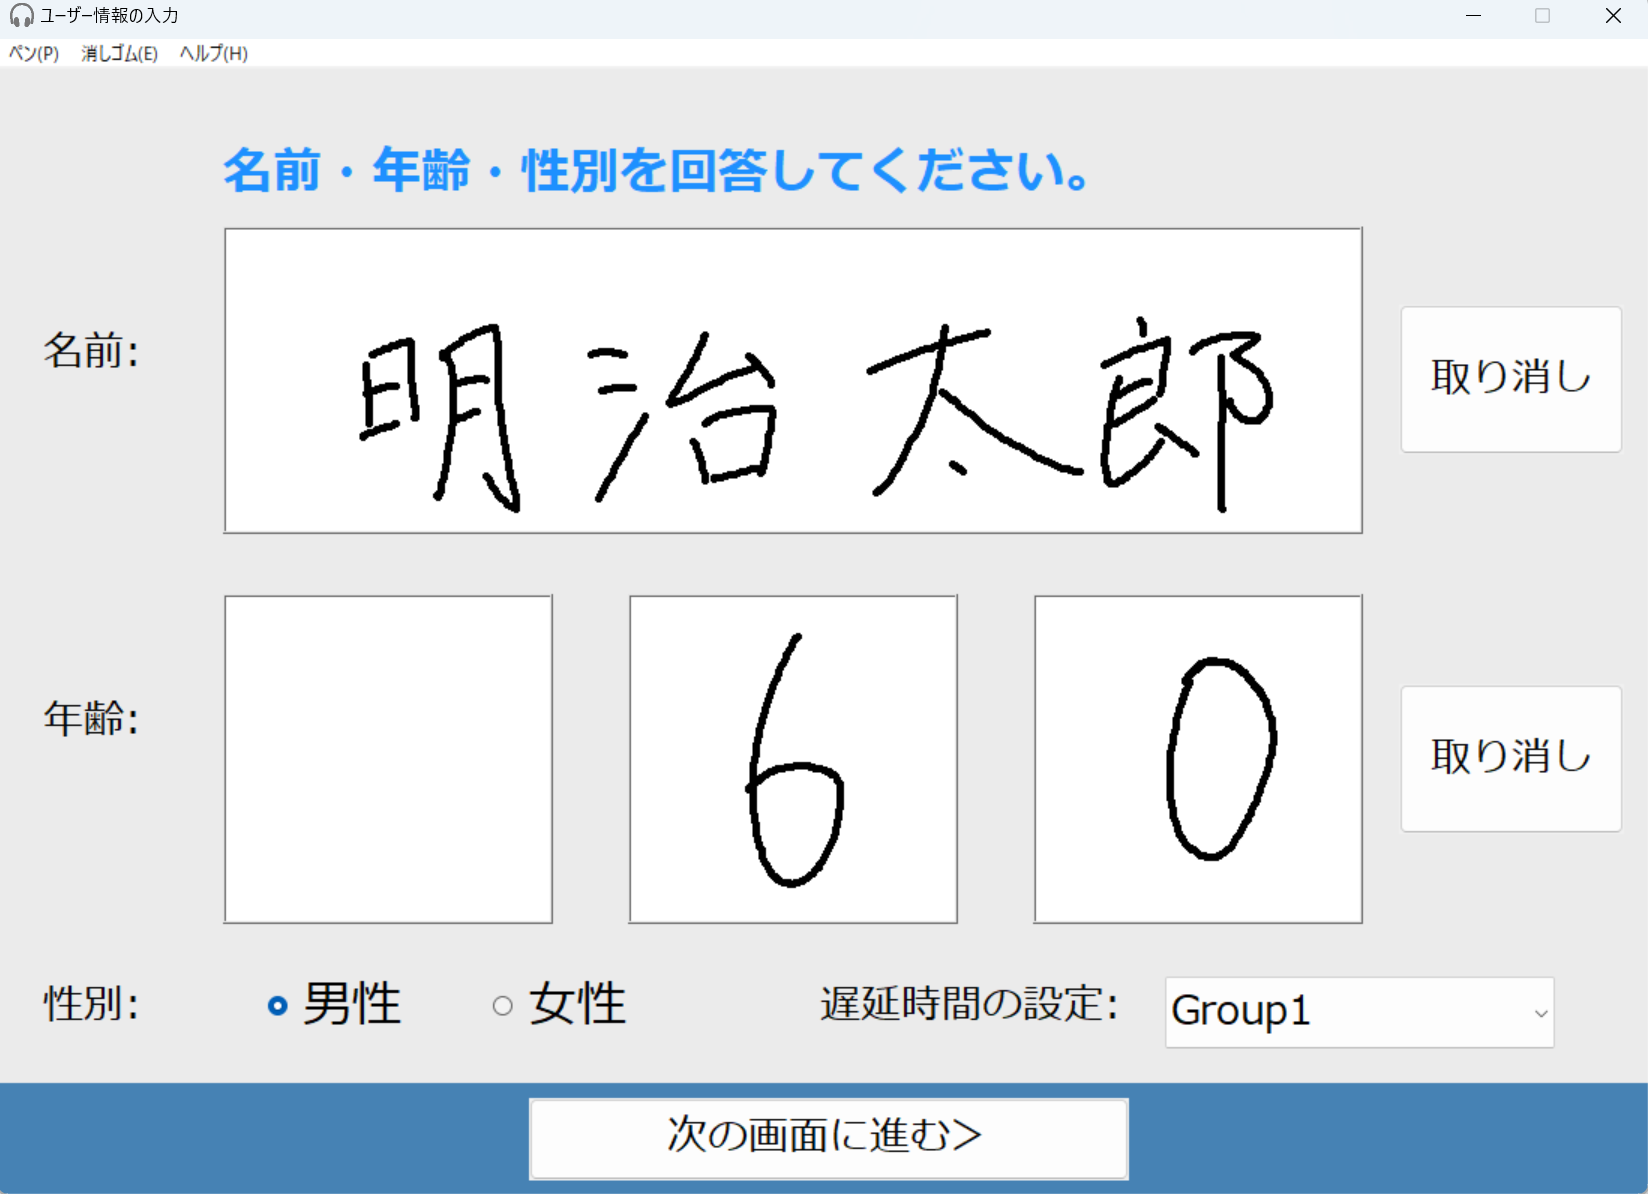
\includegraphics[scale=0.25]{figures/Syukann/gamen_1.png}
  \caption{最初の画面}
  \label{fig:1_userInterface}
\end{figure}
\begin{figure}[tbp]
  \centering
  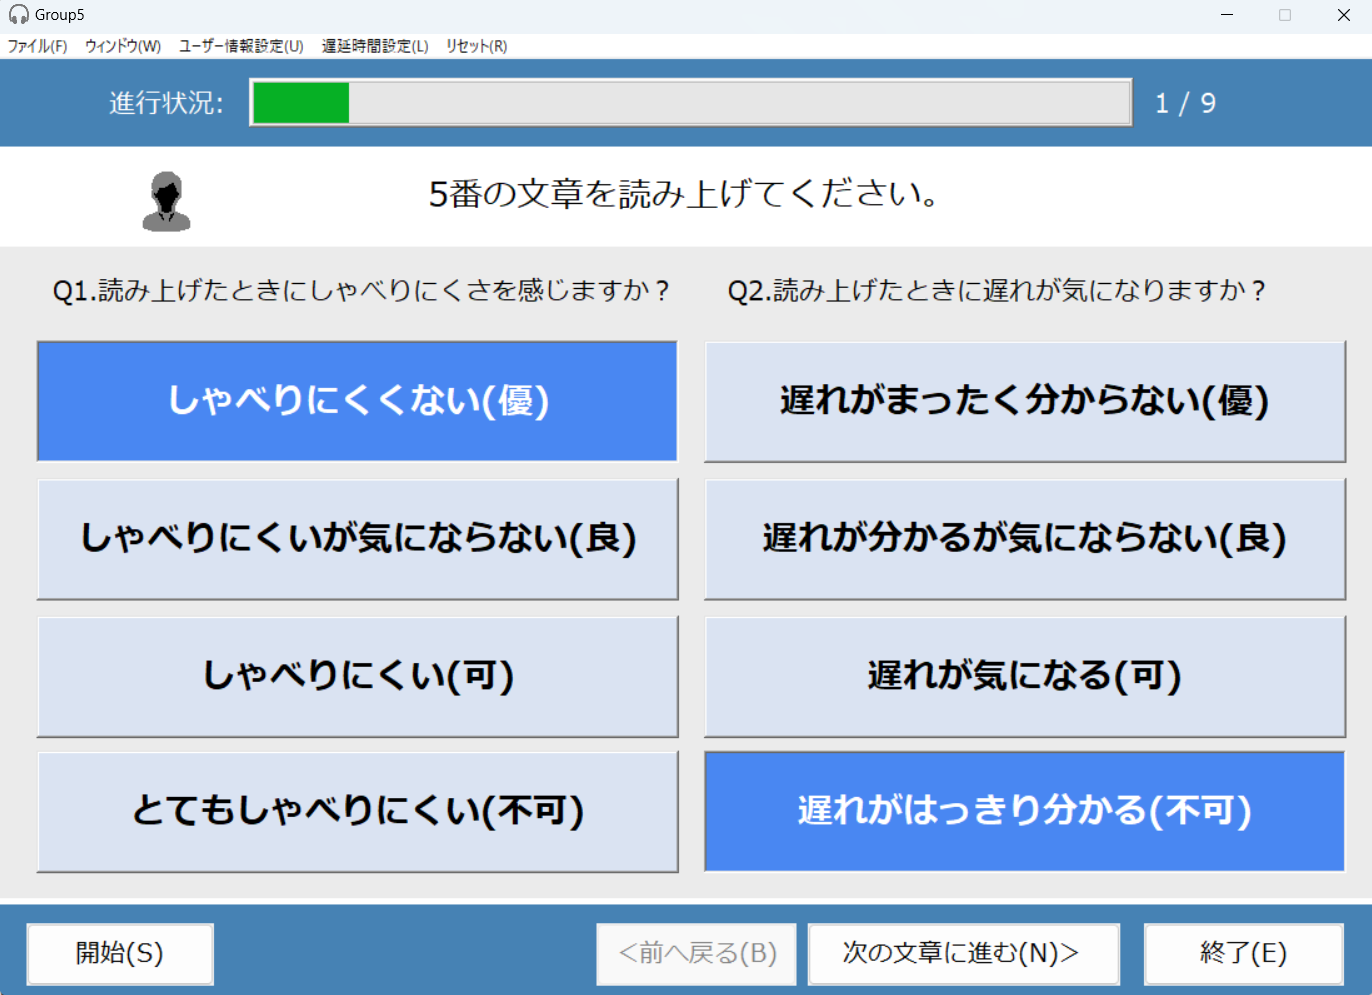
\includegraphics[scale=0.25]{figures/Syukann/app_2.png}
  \caption{2つ目の画面}
  \label{fig:2_userInterface}
\end{figure}
\begin{enumerate}[leftmargin=*]
  \item 高齢者が使用することを想定し,タッチパネルのように名前と年齢を描画できる機能(3.1.1節参照)
  \item 被験者の名前と年齢,性別,遅延時間の設定が書かれている画面をキャプチャすると同時にそれらを外部ファイルに書き込む機能(3.1.2節参照)
  \item 読む文章の番号の順番をランダムに定義し,画面上に表示する機能
  \item 2つの質問に対するそれぞれ4つの回答項目をプッシュボタンとして表示し,押下された結果を(1)と同じ外部ファイルに書き込む機能(3.1.3節参照)
\end{enumerate}
主観評価で被験者に読んでもらう文章の番号は,文献\cite{kayama}で使用された文章を使用することを想定し,10通り用意する.そのため,(3)では,1番から10番までの番号をランダムに並び替え,画面上に表示することで,被験者に提示する.
\subsection{タッチパネルによるユーザー情報の取得}
指やペンなどの1つ以上のタッチポイントがタッチに依存するデジタイザーサーフェスに触れたときに,Windows APIの「WM\_TOUCH」メッセージがウィンドウに通知される.「WM\_TOUCH」イベントは,タッチ入力に関する情報を含んでおり,アプリケーションはこのイベントを処理して,タッチ操作に応じたアクションを実行することができる.このアクションには,例えばタッチするスクリーン上の位置,タッチの圧力,動きなどの情報が含まれる.このイベントを取り扱うためにまず,ウィンドウ作成時にRegisterTouchWindow()関数を使用してアプリケーションがタッチイベントを受けとることができるようにする.その後,ウィンドウプロージャで「WM\_TOUCH」メッセージ内の処理を行うことにより,タッチパネルとしての機能を実装する.「WM\_TOUCH」イベントが通知されたら以下の処理を行うように設定する.
\begin{enumerate}[leftmargin=*]
  \item ウィンドウのデバイスコンテキストのハンドルを取得し,デバイスコンテキストに新しいペンのハンドルを割り当てる.
  \item GetTouchInputInfo()関数を使用して,各タッチイベントの情報を取得する.
  \item 取得したタッチイベントの情報を元に,タッチポイントの座標を画面上の座標に変換し,タッチの位置がタッチパネル内にあるかどうかを確認する.タッチが続いている場合,以前のタッチポイントから現在のタッチポイントまで線を描画する.
  \item 各タッチポイントについて,前回のタッチポイントの位置とタッチパネルの内か外かを記録する.これにより,タッチの移動を追跡し,描画を連続的に行うことができるようにする.
  \item 描画が終わった後,使用したペンを削除し,デバイスコンテキストを解放する.
\end{enumerate}
\subsection{画面のキャプチャ}
図3.1に示したユーザーが手書きで入力した名前と年齢は,ウィンドウの画像を「次の画面に進む」というプッシュボタンをユーザーが押下したことを合図にウィンドウの画像をキャプチャし,JPEGファイルとして保存することによって記録する.画像をキャプチャする方法は,以下の手順で実装する.
\begin{enumerate}[leftmargin=*]
  \item GetDC()関数を使用して,ウィンドウのデバイスコンテキストを取得する.
  \item GetClientRect()関数を使用して,ウィンドウのクライアント領域の寸法を取得する.クライアント領域は,アプリケーションが描画できるウィンドウの部分であり,タイトルバーと境界線を除いた部分である.
  \item クライアント領域の幅と高さ,および年齢の100,10,1桁を表す3つの領域の幅と高さを計算する.
  \item CreateCompatibleDC()関数とCreateCompatibleBitmap()関数を使用して,ウィンドウ全体と3つの年齢を示す領域のメモリデバイスコンテキストおよびビットマップを作成する.
  \item BitBlt()関数を使用して,ウィンドウ全体と3つの年齢を示す領域のビットマップをメモリデバイスコンテキストにコピーする.
  \item c++のCImageクラスを使用して,ビットマップを読み込み.画像を指定したフォルダにJPEGとして保存される.そのフォルダが存在しない場合,新しく画像を保存するためのフォルダが作成される.
  \item 最後にCImageオブジェクトからビットマップを切り離し,ウィンドウのデバイスコンテキストを解放し,元のグラフィックオブジェクトをメモリデバイスコンテキストに再選択してから,ビットマップとメモリデバイスコンテキストを削除する.

\end{enumerate}
\subsection{回答の入力と出力}
2.1.1節において記述した主観調査では,「文章の読み上げ時のしゃべりにくさ」と「文章の読み上げ時の遅れの感じ方」に関する2つの質問が画面上に提示される.被験者は,これらの質問に対して,4つの選択肢の中からWindows APIにより実装したオーナーボタンを通じて回答する.ボタンが選択されると,背景色は青色に,文字色が白色になる設計となっており,これにより高齢者を含む操作に不慣れなユーザーでも,選択状態を直感的に把握できる.
また,背景色と文字色の変更は,ボタン押下時にInvalidRect()関数によって明示的にウィンドウの再描画を要求することによって実現している.ウィンドウの再描画が必要な場合,「WM\_ERASEBKGND」メッセージが受信され,ウィンドウの背景がクリアされた後,「WM\_PAINT」メッセージによってウィンドウの内容が再描画される.この2つの処理ステップが画面のちらつきを引き起こすことがあるため,「WM\_ERASEBKGND」メッセージの処理を明示的にスキップし,InvalidRect()で更新する領域を8つのボタンを含む領域の中で最小限に設定する.そうすることで,背景のクリア処理を行わずに直接「WM\_PAINT」メッセージでの再描画に移行する.これにより,背景と前景の描画が一度に行われるため,ちらつきを減少させることができ,特に高齢者にとって快適な操作体験が実現できる.

また,全てのボタンの選択状況を常に監視し,両方のボタンが選択されていない場合,「次の文章に進む」ボタンを無効化する.これにより,結果の記録における誤りを防止する.さらに,調査の進行状況を示すプログレスバーを画面上部に設置し,調査の進捗状況をユーザーに視覚的にフィードバックする.「次の文章に進む」ボタン押下時には音声信号が本プリケーションを起動しているデバイスから出力され,実験者はこの音声信号による合図を受けて,ユーザーの合図を待たずに次の調査へと移行できる.アンケート終了後,ユーザーが「次の文章に進む」ボタンを押下すると,アプリケーション起動時に選択したCSVファイルに,キャプチャした画面のハイパーリンク付き画像ファイルパス,遅延時間のグループ名,読まれた文章の番号,回答結果が自動的に記録される.
既存のファイルであれば,結果はファイル末尾に追記される.
このシステムにより,多数の被験者を対象とする実験でも,アプリケーションの再起動なしに迅速に実験を進行できるという利点がある.
% 改善すべき点
% \section{今後の課題}
% \begin{enumerate}
%   \item 結果の出力.図のhyperlinkのとこ.excel以外で開くと文字化けする.
%   \item 結果の出力.出力先ファイルが既に開かれていた場合,結果を書き込めなくなる.
% \end{enumerate}

\chapter{ボタン押し課題のシステム}
本章では,遅延聴覚フィードバックが身体運動に与える影響を客観的に評価するための調査で行うボタン押し課題,この調査を行うために構築した調査システム及びWindowsアプリケーションについて述べる.
聴覚フィードバックは遅延時間が大きくなると,発話だけでなく身体運動に影響を与えることが知られている\cite{timing-music}\cite{shimada-DAF}.
身体運動を遅延聴覚フィードバックが与える影響の調査に使用することが可能となれば,客観的なデータを計測しやすくなることが期待される.

\section{ボタン押し課題}
本研究で行う客観評価による調査では,被験者が行う課題にボタン押し課題を採用する.
この調査で採用するボタン押し課題は,ボタンを押下するときの音に遅延を発生させて被験者に聞かせながら,
被験者がメトロノームの合図音に合わせて一定の時間間隔でボタンを押下する課題を行うというものである.
このボタン押し課題は,楽器演奏のような特別な技能を必要としないため,遅延聴覚フィードバックが身体運動に与える影響を様々な年代の被験者について調査することが可能になると考えられる.
ボタン押し課題を行っているとき,被験者がボタンを押下する時間間隔を記録すると,被験者に提示するボタン押下の時間間隔が毎分60回であれば,理想的に全てのボタンを押下する時間間隔が1000[ms]となるが,人間の操作には誤差が生じる.
また,遅延聴覚フィードバックが身体運動に影響を与えていれば,このばらつきを提示するボタンを押下する音の遅延時間によって変化するものであると考えられる.
そのため,遅延聴覚フィードバックを与えている状態で被験者がボタン押し課題を行うと,ボタンを押下する時間間隔に変化が現れることが期待される.
したがって,遅延聴覚フィードバックの下で被験者がボタン押し課題を行うときのボタンを押下する時間間隔を,
様々な遅延時間で観察することで遅延聴覚フィードバックが身体運動に与える影響を客観的に評価することができると考えられる.
この調査で使用するシステムの図を図\ref{fig:button-click-system}に示し,使用機器を表\ref{table:device}に示す.
このシステムは表\ref{table:device}の使用機器と遅延聴覚フィードバックを生成する音響信号への遅延生成アプリケーション,
メトロノーム,研究室で開発したパルスジェネレーターで構成されている.
このパルスジェネレーターは,図\ref{fig:super_famicom}に示されたコントローラーのボタンが押されると,パルス信号が生成される.
生成された信号はオペアンプにより増幅され,アナログで出力された後にオーディオインターフェースにディジタル入力される.
オーディオインターフェースに信号が入力されると,ヘッドホンからクリック音が出力されるという仕組みである.
音響信号への遅延生成アプリケーションは,4.2節で述べられるものと同様である.
以下に,本研究で用いるボタン押し課題の手順と図\ref{fig:button-click-system}のシステムの動作について説明する.
\vskip.5\baselineskip
\begin{enumerate}[leftmargin=*]
\item 被験者はヘッドホンを装着し,コントローラーを手に持つ.コントローラーのA, B, C, Dいずれかのボタンを押すと,任意の遅延時間が経過した後にヘッドホンにクリック音が出力される.
\item 電子メトロノームの合図音によって,一定間隔でボタンを押下するための合図を提示し,その合図に合わせて,被験者はボタン押し課題を実施する.
ボタン押し課題で被験者がボタンを押下する回数は,アプリケーション上で実験者が設定する.
課題中,PCに保存されたWAVファイルがオーディオインターフェースを介して,実験者が指定した時間だけ遅延してヘッドホンから出力される.
この時,実験者が指定した遅延時間は被験者には非公開とする.また,音響信号への遅延生成アプリケーションは,被験者がボタンを押下する時間間隔の記録も行う.
\end{enumerate}
\begin{figure}[tb]
  \centering
  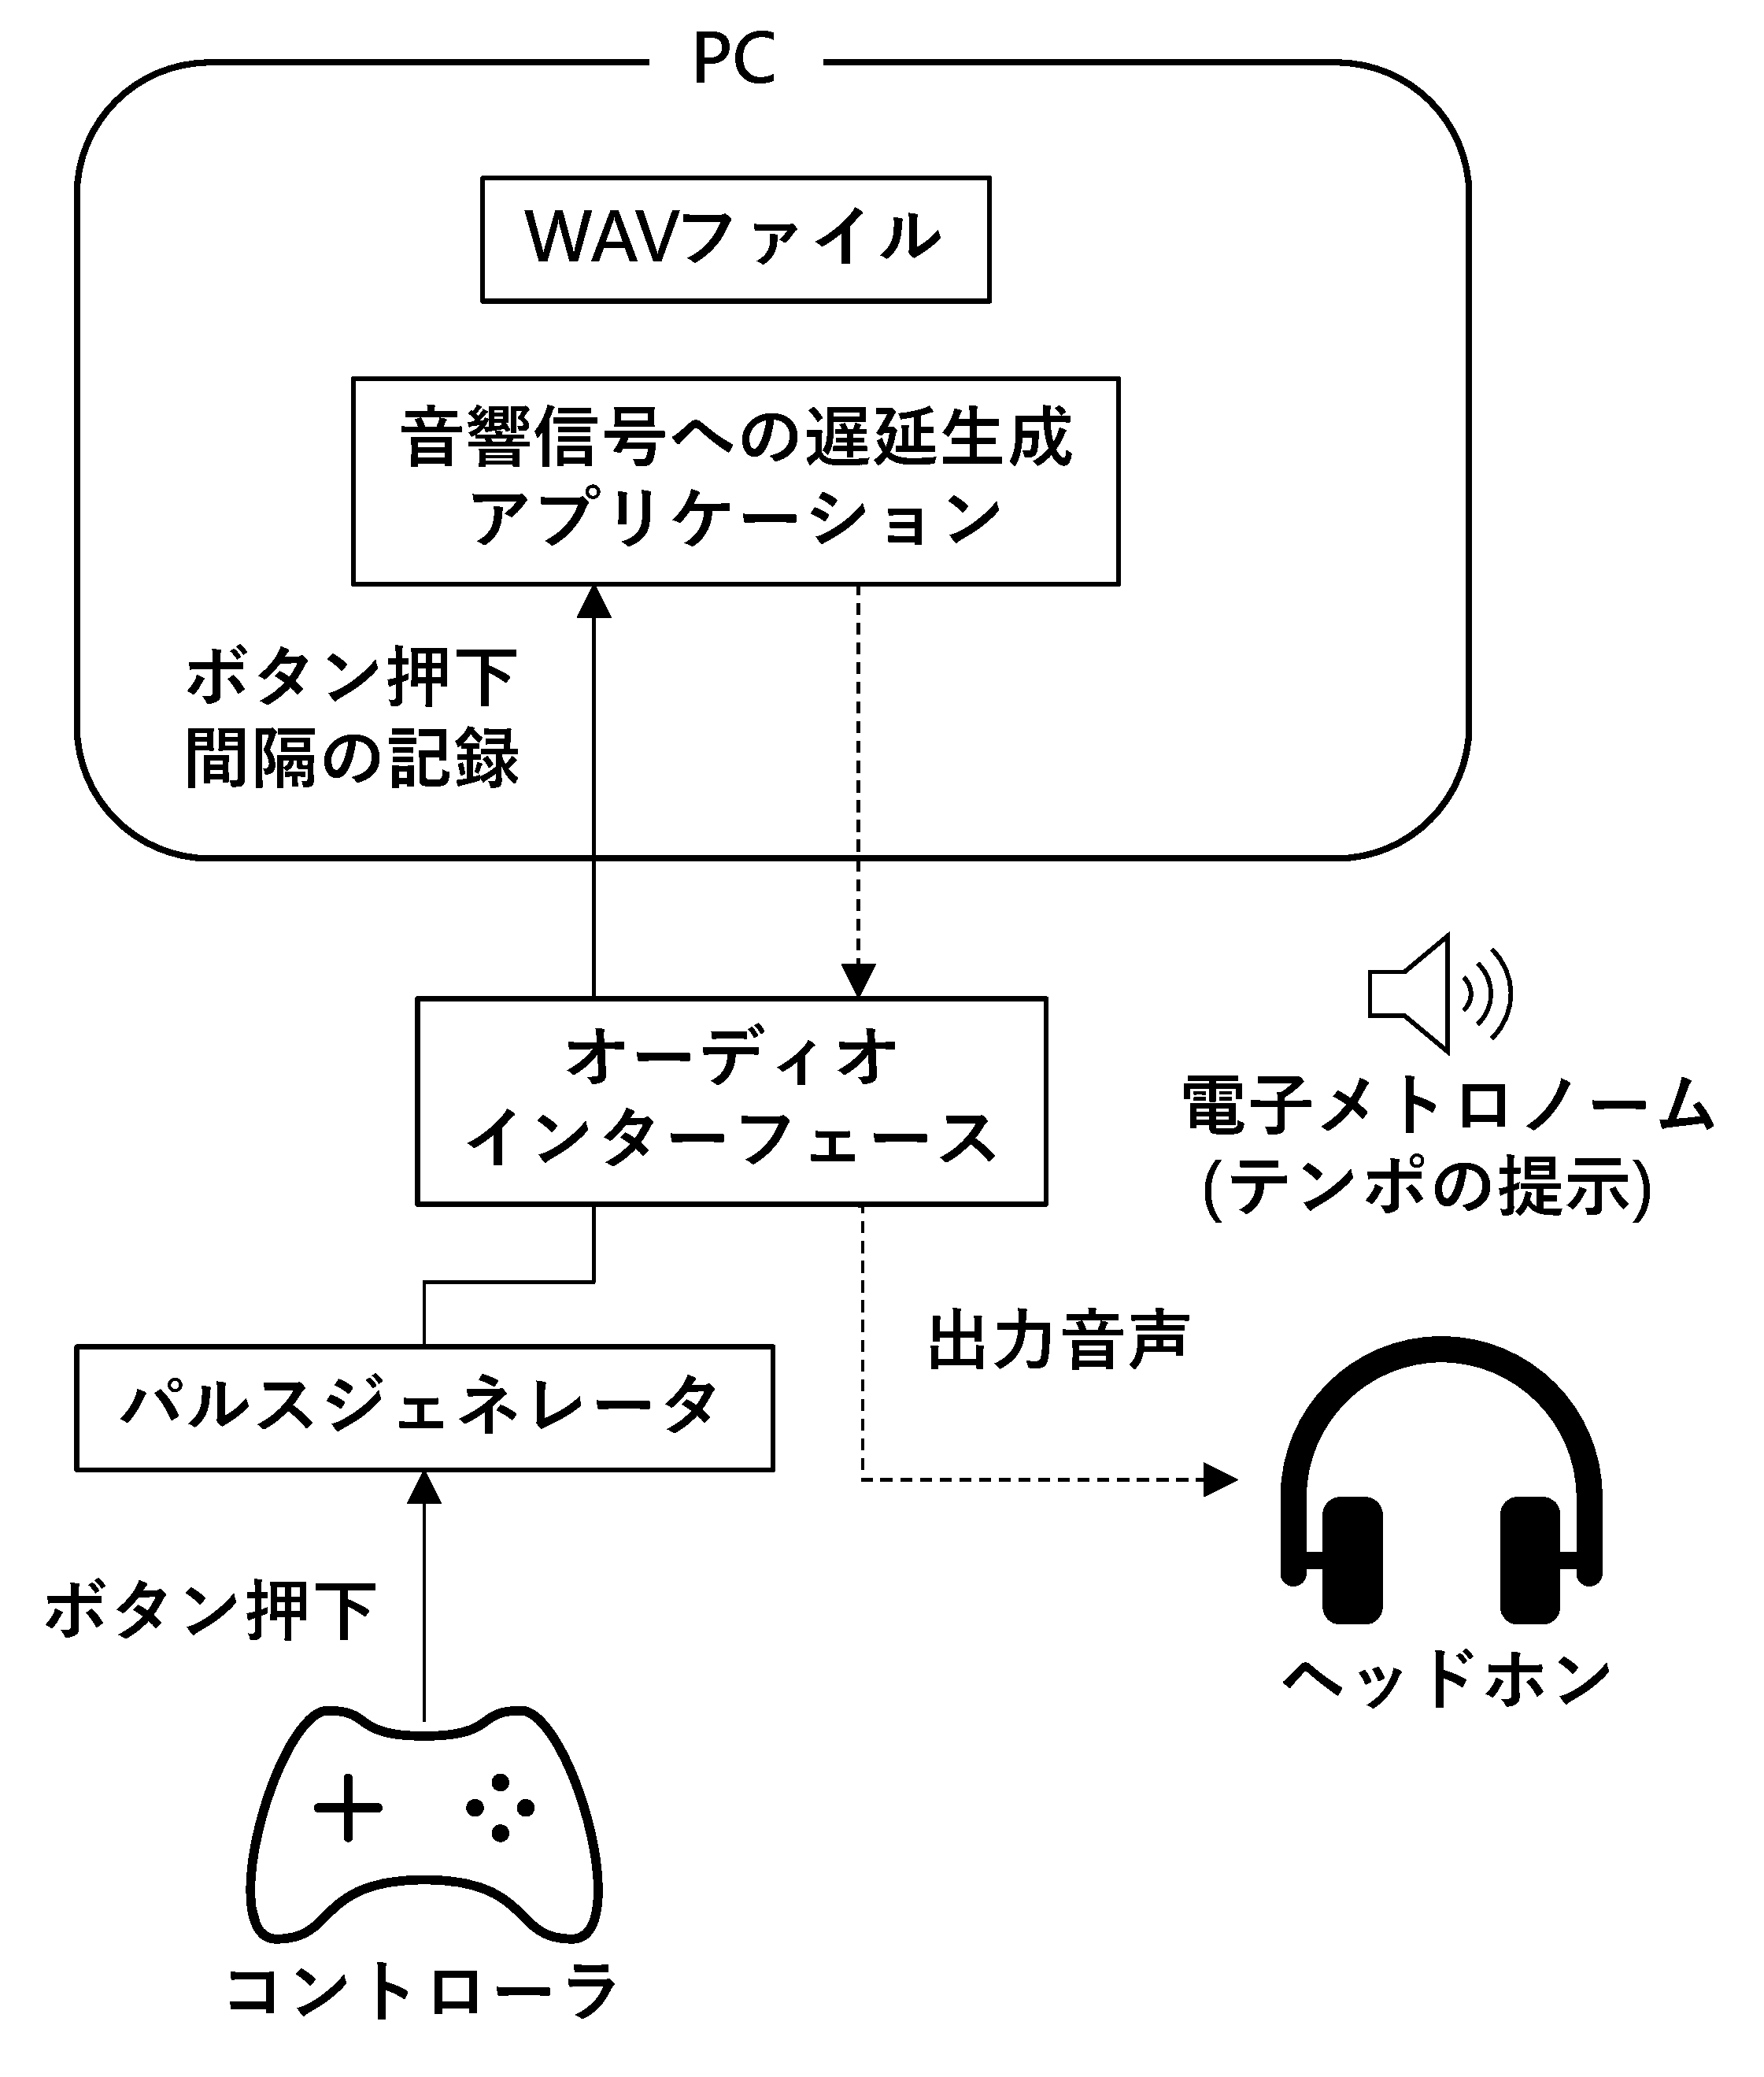
\includegraphics[scale=0.2]{figures/system_button_click.pdf}
  \caption{調査システムの構成}
  \label{fig:button-click-system}
\end{figure}
\begin{table}[tbp]
  \caption{使用機器}
  \label{table:device}
  \centering
  \begin{tabular}{lll}
    \hline
    使用機器 & 製造会社 & 製品名\\
    \hline \hline
    オーディオインターフェース & Focusrite & Scalett-Solo 3rd Generation\\
    コントローラー  & Nintendo & Super Famicom Controller\\
    開放型ヘッドホン & beyerdynamic & DT 990 PRO\\
    電子メトロノーム  & SEIKO  & DM71 Digital Metronome \\
    PC  & HP Inc. & HP ProBook 450 G7 
    % パルスジェネレーター6 & 自作 & 
\\
    \hline
  \end{tabular}
\end{table}

手順1の後,被験者が装着しているヘッドホンから出力される音声の音量調節を行う.このとき,大きな遅延時間を提示すると調査で提示する全ての遅延時間について遅れていないと判断してしまう可能性が発話に関する調査で指摘されている\cite{Soturonn-takahashi}.
そのため,音量調節時に音響信号への遅延生成アプリケーションで指定する遅延時間は,一般的に遅延を感じないとされている10[ms]以下のものとする.
また,音量調節時にヘッドホンから音声を出力している間,被験者には遅延のない音声を出力していると説明する.
音量調節が完了したら,練習としてメトロノームの合図音に合わせて20回から40回ボタンを押下してもらい,実験の内容を理解させる.
上記の手順によって記録されるボタンを押下する時間間隔及び,5章で説明する評価指標を用いて評価を行う.
\section{音響信号への遅延生成アプリケーション}
本研究で使用する音響信号への遅延生成アプリケーションは,Microsoft社が提供する統合開発環境であるVisual Studio 2022を用いてC++で開発する.このアプリケーションの表示例を図\ref{fig:app_kyakkann}に示す.
図\ref{fig:app_kyakkann}は,ボタン押し課題を開始し,アプリケーションのスタート直後の状態である.
被験者がボタンを押すと,押した時刻と直前に押した時刻からの経過時間[ms]が画面左側のエディットボックス内に書き込まれる.
実験が終了し,実験者が「ファイルへの出力」というプッシュボタンをクリックすると,実験者が指定したCSVファイルに結果が書き込まれる.
そして,開発したアプリケーションのソースコードを付録Cに掲載する.以下にアプリケーションの主な機能を示す.
\begin{enumerate}[leftmargin=*]
\item 任意の外部ファイルから複数の遅延時間を設定する機能
\item 実験者が画面上のコンボボックスで指定した時間だけ遅延させる機能(4.2.2項参照)
\item 被験者がボタンを押下する時間間隔を記録する機能(4.2.3項参照)
\item 被験者が押下するボタンの押下回数が実験者がアプリケーション上で指定した回数に到達したら合図音の出力を一時的に停止する機能
\item (3)で述べた記録とアプリケーション上での設定内容,被験者情報を外部ファイルに書き込む機能
\end{enumerate}
\begin{figure}[tb]
  \centering
  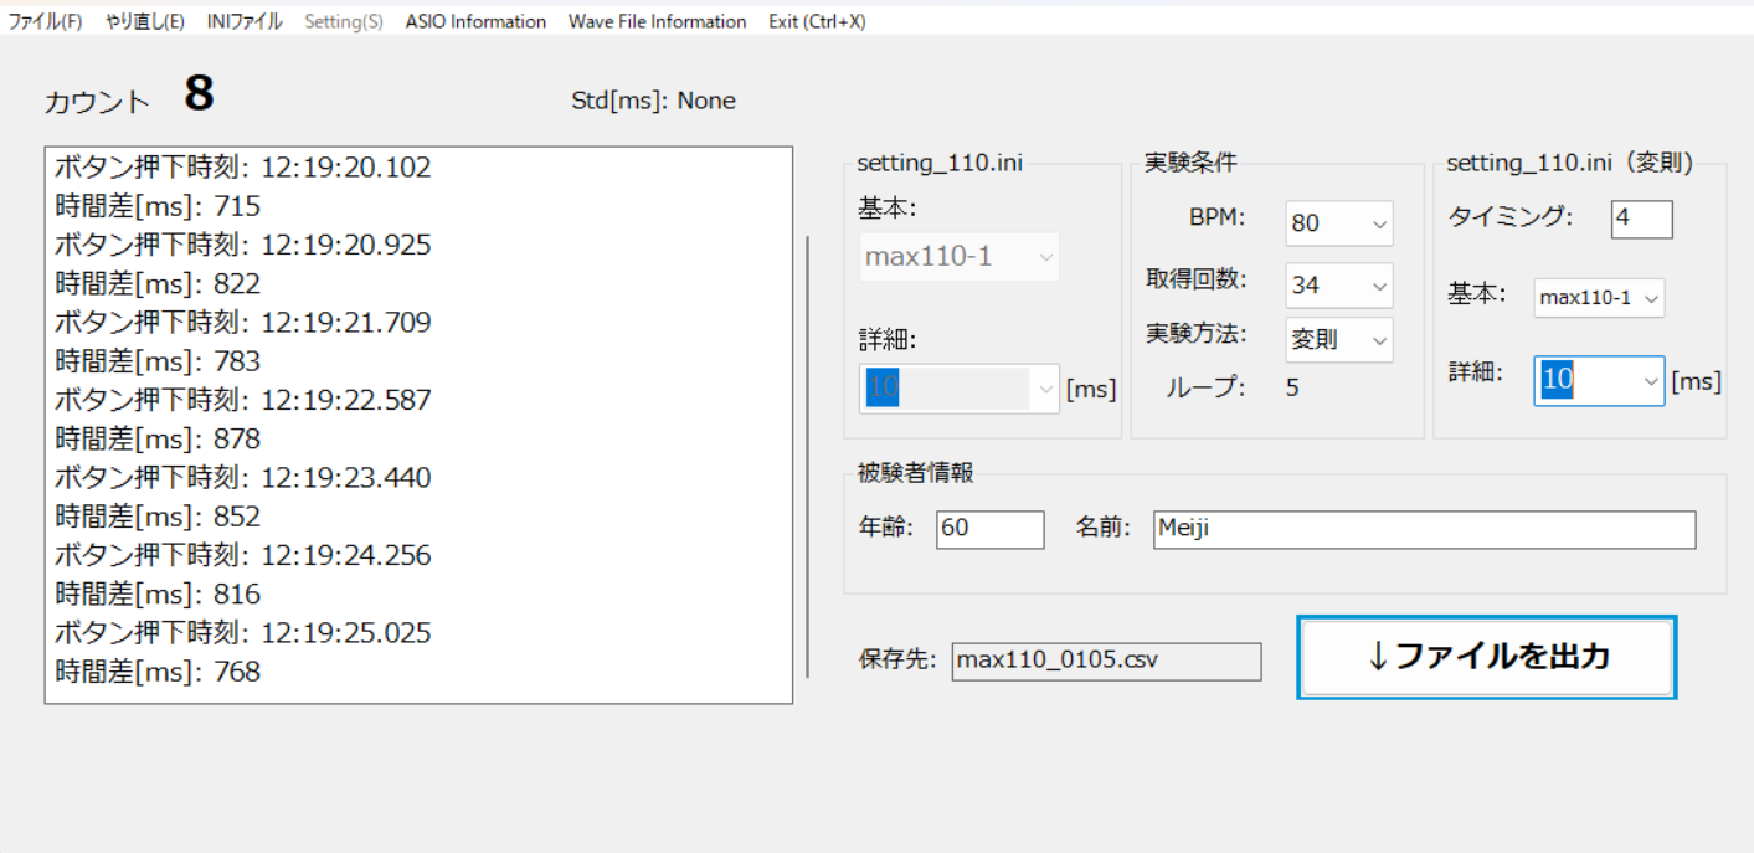
\includegraphics[scale=0.4]{figures/Apprication/App_kyakkann.pdf}
  \caption{実験開始直後の音響信号への遅延生成アプリケーションの画面}
  \label{fig:app_kyakkann}
\end{figure}
(1)はWindowsで主に使用されるINI(Initialization)ファイル形式を採用している.
遅延時間の一覧をINIファイルに予め設定し,アプリケーションから任意のINIファイルを選択し読み込むことで,
コンボボックスから遅延時間を選択する機能を実現している.
(4)は,ボタンの押下回数が指定した回数に到達したら到達したことを示すメッセージボックスを表示させることで,アプリケーションがEnterキーかOKボタンの入力を受け付けるまで合図音の出力を停止する機能である.
(5)は,被験者がボタンを押下する時間間隔を記録する機能である.
また,コンボボックスで選択された遅延時間をエディットボックスで指定したタイミングで発生させることも可能である.
さらに,選択された遅延時間に基づき遅延を発生させ,ボタンの押下回数が指定した回数に達し結果がファイルに書き込まれると,
コンボボックスの選択項目は自動的に次に移行する.
この機能により,ボタン押し課題はINIファイルの選択と結果を出力するプッシュボタンの押下のみで実施可能である.
\subsection{ASIOにおける音声の入出力}
本研究で開発するアプリケーションは,オーディオドライバにASIOを用いている.そこで,ASIOにおける音声の入出力方法について説明する.
ASIOではマルチバッファリングの切り替えを独自のコールバック関数で行う.独自のコールバック関数を用いることで,
バッファの切り替えはオーディオインターフェースによって行われるため,OSの影響を受けないという利点がある.
音声の入出力のシステムの動きを図\ref{fig:delay_theory}に示す.
入力で2つのバッファ,出力で2つのバッファを利用しそれぞれでダブルバッファリングを行う.
最初の入力バッファを入力バッファ1,次の入力バッファを入力バッファ2とし,最初の出力バッファを出力バッファ1,次の出力バッファを出力バッファ2とする.
それぞれ,音声の同時入出力が行われる前に0に初期化しておく.入力バッファ1に入力信号の格納が開始した時点から音声が出力される時点までの仕組みを以下に示す.
\begin{enumerate}[leftmargin=*]
\item はじめに入力バッファ1に入力信号が格納され,それと同時に出力バッファ1に格納されたデータの再生が始まる.しかし,この時点で出力バッファ1には録音データが格納されていないため,無音になる.
\item 入力バッファ1に格納されるデータ量が入力バッファ1の格納可能な最大の許容量に達したとき,ASIOでコールバック関数が呼び出され,入力バッファ1と出力バッファ1がアプリケーションに受け渡される.それと同時に,入力バッファ2への録音データの格納が始まり,出力バッファ2の再生が始まる.ここでも,はじめは出力バッファ2にはまだ録音データが格納されていないため,無音となる.これと同時に,アプリケーション側ではコールバックにより入力バッファ1のデータを出力バッファ1にコピーする.
\item 入力バッファ2に格納されるデータ量が入力バッファ2の格納可能な最大の許容量に達したとき,再びコールバック関数が呼び出され,出力バッファ1に格納された録音データの再生と入力バッファ1への入力信号の格納が開始する.
\item 手順2に戻る.
\end{enumerate}
以上を繰り返すことにより,音声の入出力を可能としている.しかし,このダブルバッファリングを用いた方法では,2バッファ分の遅延時間が常に発生する.
\subsection{任意の遅延時間後にボタン押下の合図音を再生させる機能}
任意の遅延時間が経過した後にWAVデータを再生させる機能は,ASIOにおける音声の入出力方法に基づいて実装する.
ボタン押下の合図音の再生は,ボタン押下を検知した後に呼び出されるコールバック関数内で,保存されているWAVデータを入力バッファの代わりに出力バッファに転送することで行われる.
このWAVデータの出力バッファへの転送のタイミングを遅延時間ごとに調整することで,任意の遅延時間後にボタン押下の合図音を再生させる機能を実現させる.
また,図\ref{fig:delay_theory}のようにボタンの押下検知からWAVデータの再生までに少なくとも2つのバッファ分の遅延が生成されることになる.
バッファサイズが小さいほど,より高精度な遅延時間の設定が可能となる.
オーディオインターフェースのバッファサイズを$n$[points],サンプリング周波数を$f_{s}$[Hz],ASIOにおけるインターフェイスに固有の入力遅延を$i$[ms],ASIOにおけるインターフェイスの固有の出力遅延を$o$[ms],
% その他の遅延時間を$x$[ms],
所望の遅延時間を$d$[ms]とすると,遅延時間の生成は以下のような手順で実現される.
\begin{enumerate}[leftmargin=*]
  \item 初めに式\ref{eq:my_equation}に基づき,WAVデータのコピー時刻$T$を定義する.この時刻$T$は,ボタン押下の検出後,何回目のコールバック関数の呼び出し時にWAVデータをコピーするかを示す指標である.生成したい遅延時間$d$[ms]は,実験者がアプリケーション上で指定する.
\begin{equation}
T = \left\{ d - (i + o) \right\} \times n \times \left( \frac{f_s}{1000} \right) \label{eq:my_equation}
\end{equation}

  \item ボタンの押下を検知してから最初のコールバック関数呼び出し時を1回目として,$T-1$回目までは,入力バッファに格納されているデータを出力バッファにコピーする.このとき,入力バッファには0が格納されているため無音となる.
  \item ボタンの押下を検知してから$T$回目のコールバック関数呼び出し時になったら,入力バッファに格納されているデータの代わりにWAVデータを出力バッファにコピーしていく.
\end{enumerate}
上記の手順を踏むことにより,任意の遅延時間の生成を実現する.
\begin{figure}[h]
  \centering
  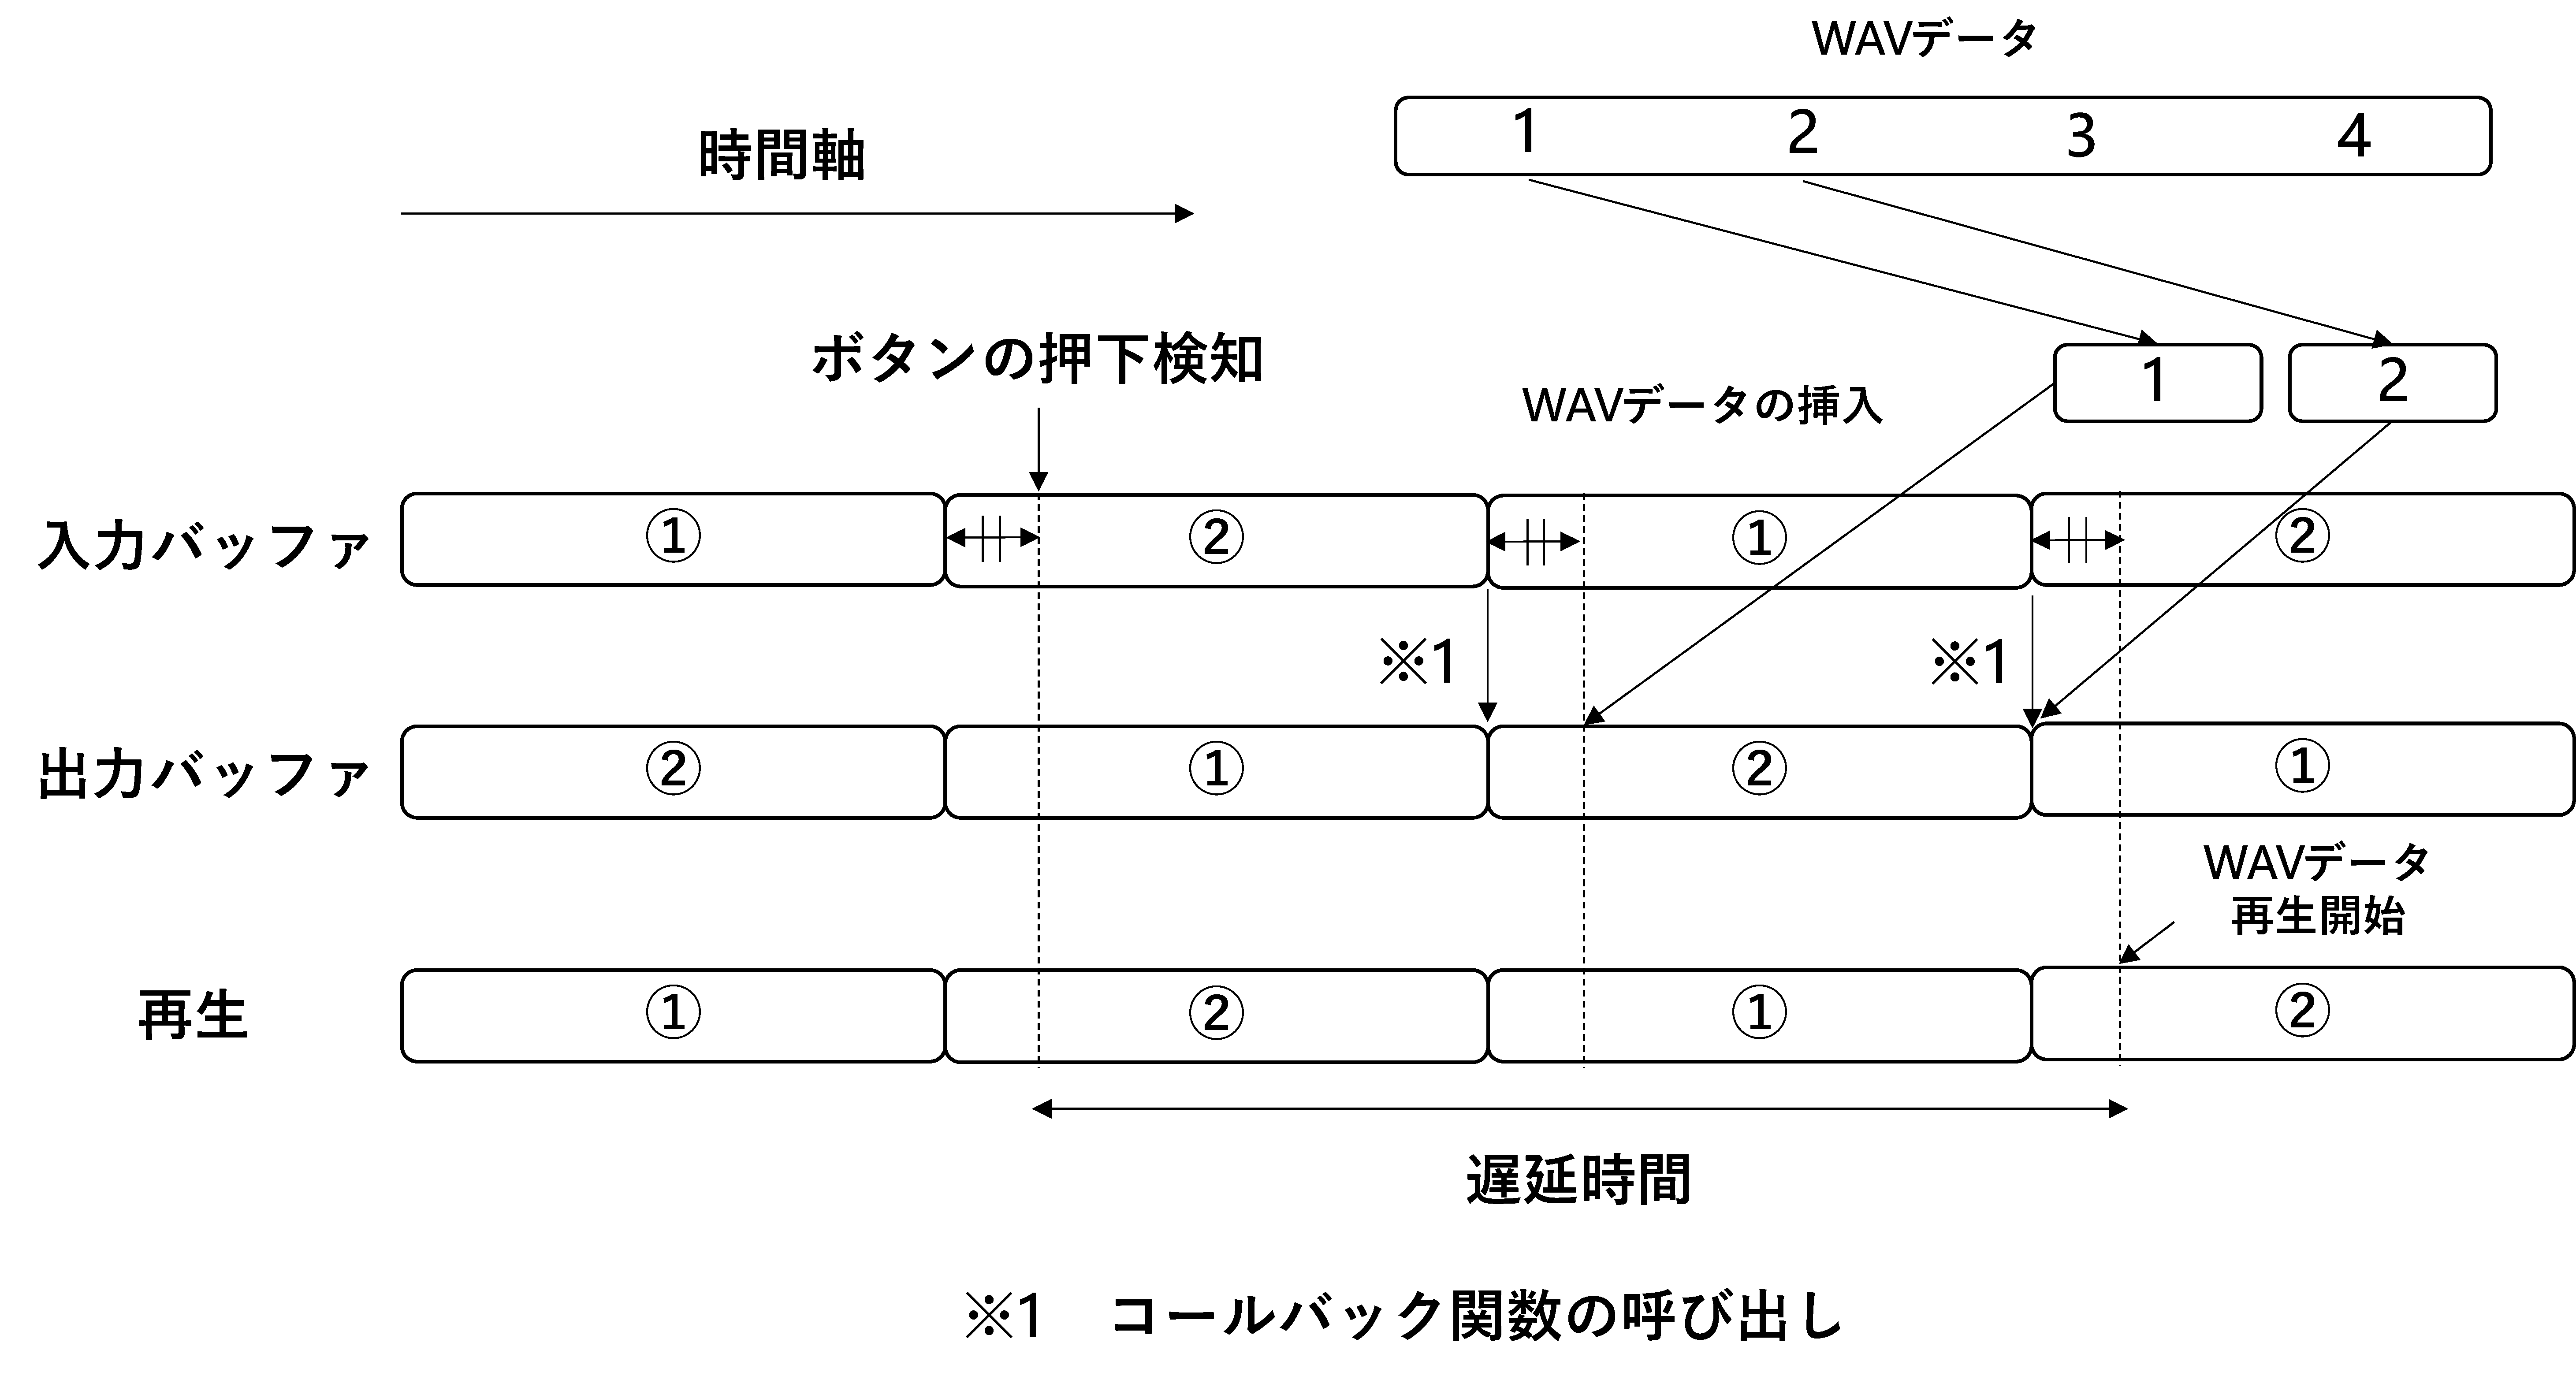
\includegraphics[scale=0.12]{figures/System/Delay_theory.pdf}
  \caption{遅延時間の生成原理}
  \label{fig:delay_theory}
\end{figure}
\subsection{ボタンの押下時間間隔を記録する機能}
ボタンの押下時間間隔を記録する機能は,ボタンを押下するごとに,ボタンの押下と押下の間の時間を計測する.
例外として,1回目のボタンの押下時間間隔は記録しないように設定する.
押下時間間隔の取得には,C++の標準ライブラリであるstd::chronoを使用する.
std::chronoは,C++11以降で使用可能な時間に関する操作を提供するライブラリである.
以下に押下と押下の間の時間を計測するための手順を示す.
\begin{enumerate}[leftmargin=*]
\item ボタン押下を検知したら,関数std::chrono::system\_clock::now()を使用してエポック(1970年1月1日0時0分0秒 UTC)からの経過時間を取得し,用意した変数Aに代入する.
\item 再びボタンの押下を検知したら,変数Aを別の変数Bに代入し,変数Aに手順1と同様の方法でエポックからの経過時間を取得し,代入する.
\item ボタンの押下が2回目以降であれば,手順2の後に変数Bと変数Aの差を計算し,変数Cに代入する.
\item 関数std::chrono::duration\_cast\textless std::chrono::milliseconds\textgreater()によって変数Cをミリ秒単位の時間に変換する.
\item 手順3で変換した変数Cを随時,配列に追加していくことで全てのボタンの押下時間間隔を記録する.
\end{enumerate}
\section{生成する遅延時間の正確性の調査}
\subsection{遅延時間の測定方法}
4.2節で述べたアプリケーションによって生成された遅延時間の正確性を検証する目的で,遅延時間の測定を行う.
図\ref{fig:delay_check}に遅延時間測定のための接続図を示す.
測定手順は以下の通りである.
\begin{figure}[tbp]
  \centering
  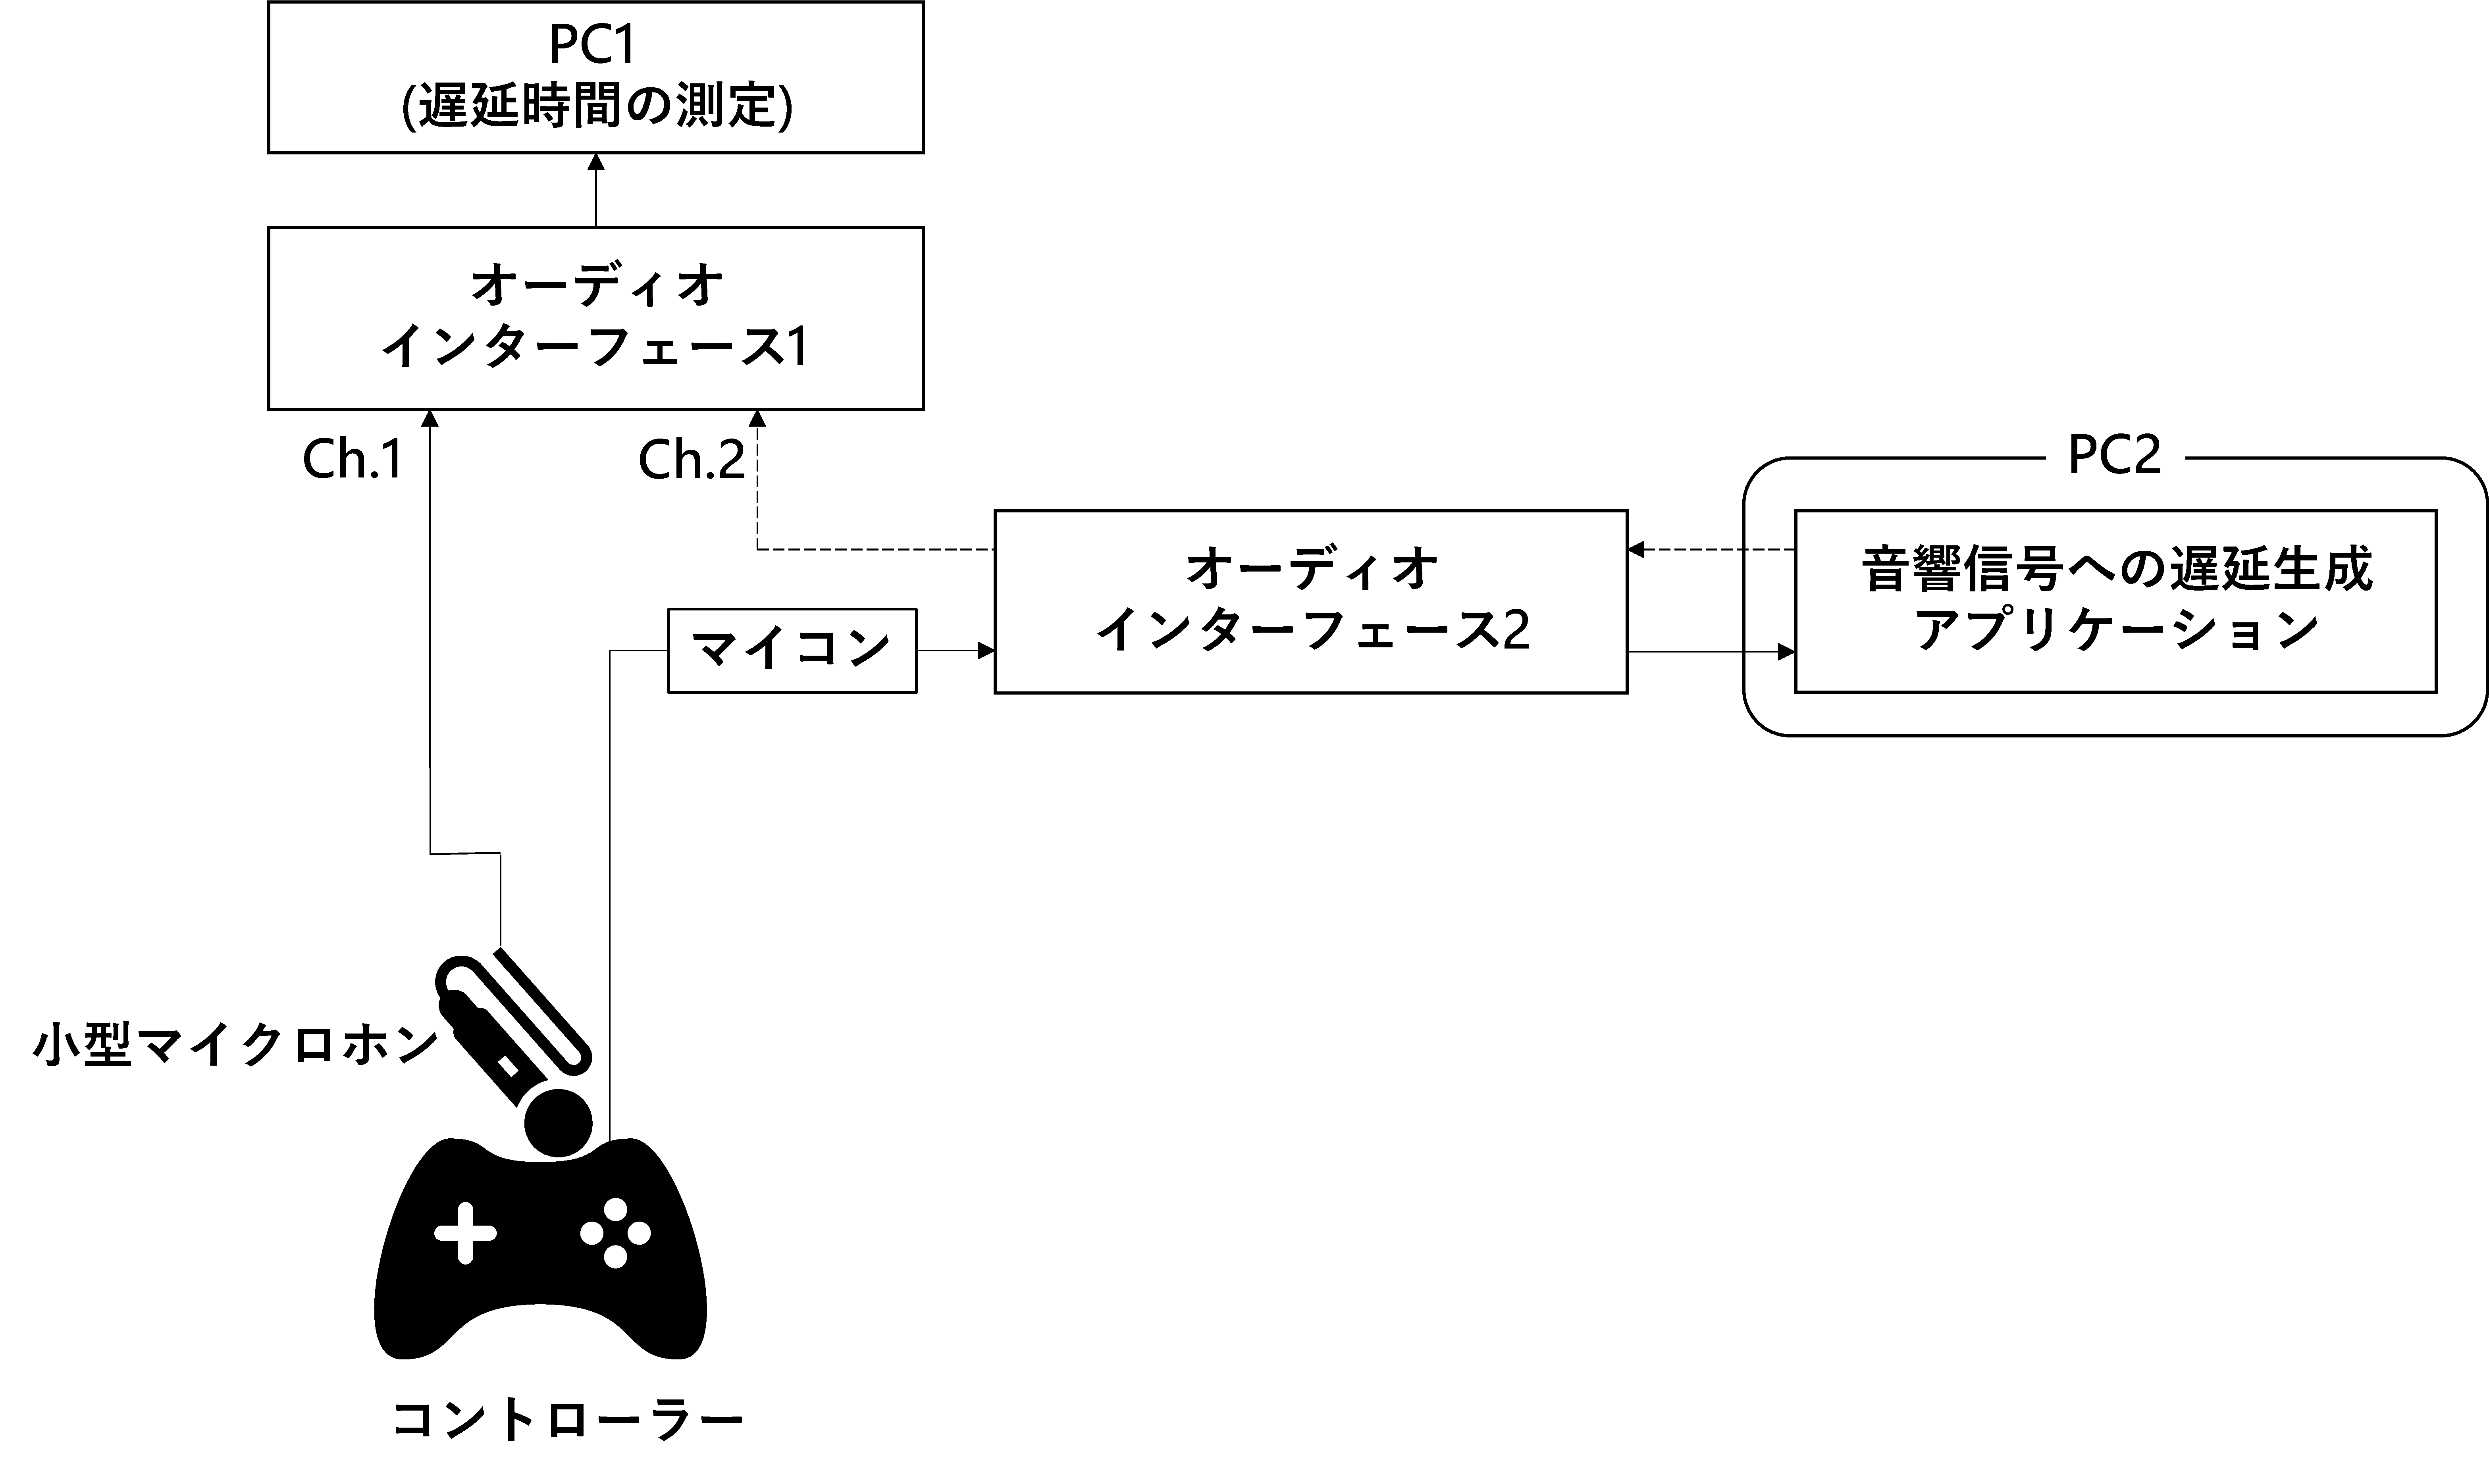
\includegraphics[scale=0.12]{figures/DelayCheck/DelayCheck_EX.pdf}
  \caption{遅延時間測定のための接続図}
  \label{fig:delay_check}
\end{figure}
\begin{enumerate}[leftmargin=*]
  \item 測定システムを図\ref{fig:delay_check}に示された構成で用意する.
  \item 遅延時間測定のためのプログラムと遅延時間生成アプリケーションが起動してから十分に時間が経過した後,実験者がボタンを押下する.
  \item 図\ref{fig:super_famicom}のような小型マイクロホンを取り付けたコントローラーから取得した音をオーディオインターフェース1のチャンネル1へと入力する.
  \item コントローラーのボタンを押下することで,遅延生成アプリケーションを介して出力される音声をオーディオインターフェース1のチャンネル2へ入力する.
  \item 遅延時間測定のためのプログラムの実行後にチャンネル1に入力された信号の開始点から1000点目の点から6000点目の点の信号の振幅の標準偏差を求める.
  チャンネル1において,標準偏差の2倍を超えた点を検出し,チャンネル1に入力された信号(小型マイクロホンから取得した音響信号)の開始点とする.
  \item チャンネル2においても同様に,標準偏差の2倍を超えた点を検出し,
  これをチャンネル2における信号(アプリケーションによって生成された音響信号)の開始点とする.
  \item それぞれの開始点の時間差を計算し,これを遅延時間[ms]として算出する.
\end{enumerate}
\begin{figure}[bt]
  \centering
  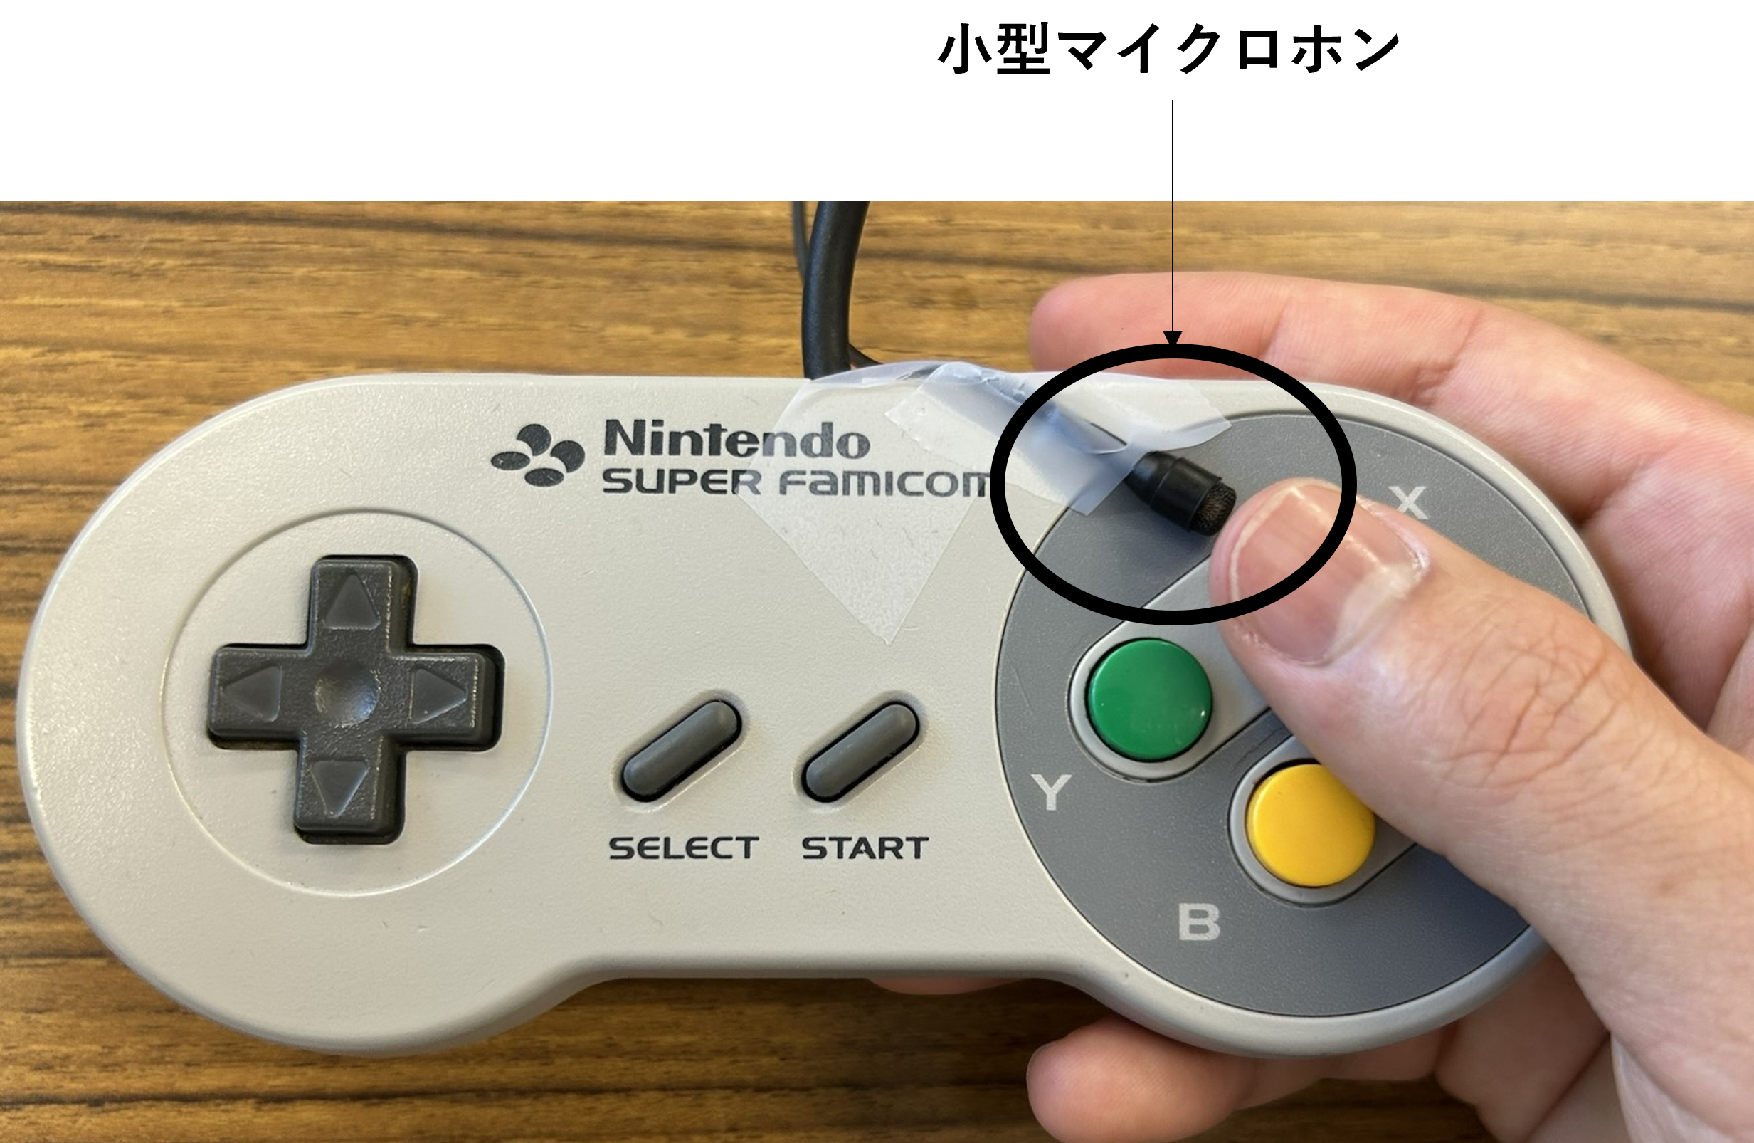
\includegraphics[scale=0.35]{figures/DelayCheck/SuperFamicom_delayCheck.pdf}
  \caption{小型マイクロホンを装着しているコントローラー}
  \label{fig:super_famicom}
\end{figure}
システムの動作確認は,CPU使用率を100%に保つ重い計算を実行する状態と,通常のCPU負荷がない状態の両方で行う.
これにより,他のアプリケーションによるCPU占有が生じてもシステムが正常に機能するか否かを検証する.
遅延時間の測定は合計10回行い,遅延時間の理論値と実測値の差の絶対値の平均および実測値の標準偏差を算出する.
使用機器の詳細を表\ref{table:device_delay_check}に示す.
設定されたバッファサイズはオーディオインターフェースで設定可能な最小のバッファサイズである16,サンプリング周波数は48[kHz],量子化ビット数は16[bit]とする.
遅延時間は10-40[ms]の範囲では5[ms]ずつ,40-150[ms]の範囲では20[ms]ずつ変化させ,各場合において遅延時間を測定する.
% \subsection{測定条件}
\begin{table}[tbp]
  \caption{測定に使用した機器}
  \label{table:device_delay_check}
  \centering
  \begin{tabular}{lccc}
    \hline
    実験装置 & 製造会社 & 製品名\\
    \hline \hline
    オーディオインターフェース1  & Roland & Duo-Capture EX\\
    オーディオインターフェース2  & Forcusrite & Scarett-solo 3rd Generation\\
    遅延時間生成用のPC  & HP Inc. & HP ProBook 450 G7\\
    遅延時間測定用のPC  & HP Inc. & HP Pavilion Laptop 14-dv2xxx\\
    マイクロホン  & DPA Microphones & IMK-SC4060
\\
    \hline
  \end{tabular}
\end{table}

\subsection{測定結果}
表\ref{table:delay_check_result}に測定結果を示す.
表\ref{table:delay_check_result}よりCPU利用率が平常時においては,理論値の誤差と実測値の差が小さいことから,アプリケーションの正常な動作が確認された.
一方で,CPU利用率が100%の状態では,理論値と実測値の差および実測値の標準偏差が著しく増加することが確認された.
これは,本研究で開発されたアプリケーションが,CPU利用率が100%の際には正常に機能しないことを示している.
したがって,本研究で開発されたアプリケーションを用いてボタン押し課題を実施する際には,CPU利用率が100%に至らないよう注意が必要であり,
実験を行う研究者は,他のアプリケーションを終了させる等の措置を講じ,CPU利用率が100%にならないように慎重に実験を進める必要がある.
そのため,本研究で実験を行う際にはCPU利用率が100%にならないように注意を払い,実験を行うこととする.
\begin{table}[tbp]
  \caption{測定結果}
  \label{table:delay_check_result}
  \centering
  \begin{tabular}{ccc}
    \hline
    \begin{tabular}{c}
      CPU \\ 利用率
    \end{tabular}
    & 
    % \begin{tabular}{c}
    %   オーディオ入出力の \\ バッファサイズ
    % \end{tabular}
    % &
    % \begin{tabular}{c}
    %   サンプリング周波数 \\ {} [kHz]
    % \end{tabular}
    % &
    % \begin{tabular}{c}
    %   量子化ビット数 \\  {} [bit]
    % \end{tabular}
    % &
    \begin{tabular}{c}
      理論値と実測値の \\ 差の絶対値の平均[ms]
    \end{tabular}
    & 
    \begin{tabular}{c}
      実測値の \\ 標準偏差[ms]
    \end{tabular}
     \\
    \hline \hline
    平常時  & 0.129 & 1.23\\
    100[%]時 & 5.08 & 4.93\\
    \hline
  \end{tabular}
\end{table}

\chapter{遅延聴覚フィードバックが身体運動に与える影響の評価方法}
本章では,遅延聴覚フィードバックが身体運動に与える影響の評価方法を述べる.
4章で説明した方法で被験者がボタンを押下する時間を記録すると,被験者に提示するボタンの押下の時間間隔が毎分60回であれば,理想的には1000[ms]の間隔でボタンが押下される.
しかし,人がボタンを押下すると理想的なボタン押下の時間間隔にばらつきが生じると考えられる.
また,遅延聴覚フィードバックが身体運動に影響を与えて入れば,このばらつきは聴覚フィードバックの遅延時間の大きさによって変化するものであると考えらえる.
そこで,このボタン押下の時間間隔のばらつきを各遅延時間で評価することで,遅延聴覚フィードバックが身体運動に与える影響を評価する.
ばらつきの評価には,分散と二乗誤差を用いる.これらの評価指標は,ばらつきが大きくなるほど値が大きくなるため,評価指標の計算結果の大小でばらつきの大きさを観察することが可能になると考えられる.
そして,これらの評価指標を算出するとき,評価指標の値の時間変化や評価に使用するデータの個数によって値が変化を比較することを想定して,これらをパラメータとして用いる.
\section{分散}
まず、ボタンを押下する時間間隔の不偏分散$s^2_{1}$は,被験者が行うボタン押下の時間間隔を用いて算出する.$s^2_{1}$は,以下の式により示される.
\begin{equation}
  s^2_a = \frac{1}{l-1} \sum_{i=k}^{k+l-1} (x_i - \bar{x}_{kl})^2
\end{equation}
ここで$l$[回]は分散を算出するために使用するデータの個数,$k$は分析するデータの最初のインデックス,$x_{i}$[ms]は,取得した$i$番目のボタンの押下時間間隔のデータ,$\bar{x}_{kl}$[ms]は,$k$番目のデータから$n$個のデータを用いて算出するボタンの押下時間間隔のデータの平均値を指す.
$s^2_{1}$において,任意の$i$で理想的な時刻にボタンが押下されなかった場合,$x_{i}$と$x_{i+1}$の両方に理想的なボタンの押下時間間隔との差異が生じる.データの平均値との差異を分析する際,大きな誤差が発生した場合,その影響で分散が過大になり,適切な評価が困難になる可能性がある.したがって,各被験者のボタンの押下時間間隔のデータの中央値を真値とする分散を検討することが有効である.中央値を真値として用いることにより,データに極端な誤差が生じた場合でも、ボタンの押下時間間隔のばらつきを適切に評価することが可能になると考えられる.各被験者のボタンの押下時間間隔のデータの中央値を真値とする分散$s^2_{2}$は,以下の式により示される.
\begin{equation}
  s^2_b = \frac{1}{l} \sum_{i=k}^{k+l-1} (x_i - M_{kl})^2
\end{equation}
を用いてここで,$M_{kl}$は,$k$番目のデータから$n$個のデータを用いて算出するボタンの押下時間間隔のデータの中央値を指す.
次に,真値を理想的なボタンの押下時間間隔とする場合を考える.例えば,ボタン押下の回数が毎分60回であれば,理想的には1000[ms]の間隔でボタンが押下される.しかし,実際の実験では,この理想的な間隔でボタンが押下されるとは考えにくく,その理想的な間隔との誤差の分散は,ばらつきが増加するとともに大きくなると推測される.理想的なボタンの押下時間間隔との誤差の分散$s^2_{3}$は,以下の式により示される.
\begin{equation}
  s^2_c = \frac{1}{l} \sum_{i=k}^{k+l-1} (x_i - T)^2
\end{equation}
% \section{標準偏差}
% まず,ボタンを押下する時間間隔の標準偏差$s_{1}$[ms]は,記録するボタンを押下する時間間隔を用いて算出する.$s_{1}$は次式で表される.
% \begin{equation}
%   s_1 = \sqrt{\frac{1}{n-1} \sum_{i=k}^{k+n-1} (x_i - \bar{x}_{kl})^2}
% \end{equation}
% \begin{equation}
%   s_2 = \sqrt{\frac{1}{n} \sum_{i=k}^{k+n-1} (x_i - M)^2}
% \end{equation}
% \begin{equation}
%   s_3 = \sqrt{\frac{1}{n} \sum_{i=k}^{k+n-1} (x_i - T)^2}
% \end{equation}
\section{二乗誤差}
本節では,聴覚フィードバックの遅延が変則的に発生する場合のばらつき評価について検討する.遅延が$t$の倍数に到達した際のみ発生する状況を想定し,$t$の倍数に到達する直前のボタン押下間隔と直後のボタン押下間隔のデータの差の二乗平均(MSE)が,遅延聴覚フィードバックがボタン押下間隔に与える影響を反映すると仮定する.遅延時間が増加するにつれて,MSEも増加すると予測される.
MSEを算出する際に用いる誤差の総数を表す関数$f(n)$と,使用するデータの最後のインデックスを示す関数$s(n)$は,ボタン押下回数$n$を用いて以下の式で表される.

\begin{equation}
f(n) = \left\lfloor \frac{n-t-1}{t} \right\rfloor + 1
\end{equation}
\begin{equation}
s(n) = \left\lfloor \frac{n-t-2}{t-1} \right\rfloor
\end{equation}

ここで,$\left\lfloor x \right\rfloor$は$x$を超えない最大の整数を示す.

これらの関数を用いて,MSEは次の式で定義される.

\begin{equation}
MSE = \frac{1}{f(n)} \sum_{i=0}^{s(n)} (d_{t-1+ti} - d_{t+ti})^2
\end{equation}

ここで,$d_{t-1+ti}$は$t$の倍数に達する直前のボタン押下間隔,$d_{t+ti}$は$t$の倍数に達した直後のボタン押下間隔のデータを示$MSE$,聴覚フィードバックの遅延による影響を定量的に評価することが可能となると考えられる.
さらに,$t$の倍数に到達する直前のボタン押下時間間隔と到達した直後の間隔との誤差の中央値(これ以降$MedSE$と呼ぶことにする)での評価を検討する.この計算法により,誤差の極端な値が存在しても適切なばらつきの評価が行える可能性がある.誤差の中央値$MedSE$は以下の式で定義される.

\begin{equation}
MedSE = Med((d_{3}-d_{4})^2, (d_{7}-d_{8})^2, \ldots, (d_{t-1+ts(n)}-d_{t+ts(n)})^2)
\end{equation}

この式では,$Med()$は中央値を計算する関数であり,括弧内の各項は$t$の倍数に到達する直前後のボタン押下間隔の差の二乗を示す.このように,$MedSE$を用いることで,データの極端なばらつきによる影響を抑えつつ,遅延聴覚フィードバックの効果をより適切に評価することが期待される.

% \section{絶対値誤差}
% \begin{equation}
%   MAE = \frac{1}{f(n)} \sum_{i=0}^{s(n)} |d_{3+4i} - d_{4+4i}|
% \end{equation}

\chapter{身体運動のばらつきを評価するための最適な実験条件}
4章で述べたボタン押し課題でボタンの押下時間間隔を記録すると,聴覚フィードバックに遅延がない場合でも理想的なボタンの押下時間間隔にはならずいくらかのばらつきが発生する.
これは,遅延聴覚フィードバックが身体運動に与える影響の調査において発生する本質的なばらつきであると考えられる.
そのため,聴覚フィードバックに遅延がない場合でのばらつきが小さくなるような実験条件を用いれば,遅延による影響がより顕著に現れることが期待される.
そこで,本章ではこの調査における最適な実験条件を明らかにするために,以下の実験から実験条件によるばらつきの変化を調査した.
\begin{enumerate}[leftmargin=*, label=実験(\arabic*)] % ラベルの設定
  \item メトロノームの合図音のBPMを変化させたときのボタンの押下時間間隔のばらつきの変化を調べる.
  \item 分散の計算に用いるデータの個数の違いによるばらつきの変化を調べる.
\end{enumerate}
実験(1)と実験(2)では,聴覚フィードバックの遅延時間を一般的に影響のない遅延時間とされている10[ms]に設定した.
\section{ボタンを押下する間隔の最適な条件}
この実験では,1分間にボタンを押下する回数を70回から110回までの5種類に変化させる.20代の被験者8人を対象に調査を行った.
図\ref{fig:bpm}にボタンを押下する間隔と評価指標の関係を示す.
この図から1分間に80回の間隔でボタンを押下するときが最も評価値が小さいことがわかる.
このため,これ以降の実験では,ボタンを押下する時間間隔を1分間に80回とする.
\begin{figure}[b]
  \centering
  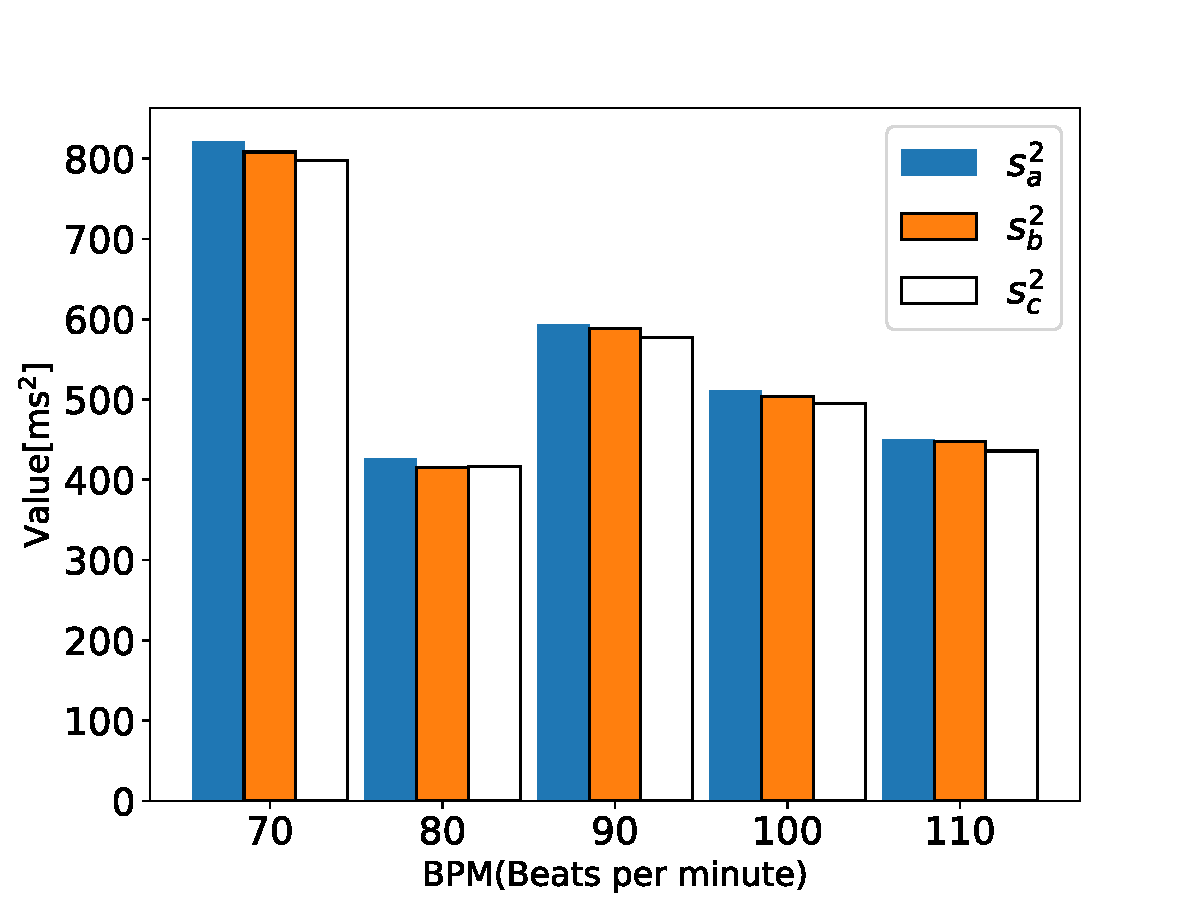
\includegraphics[scale=0.6]{figures/Yobi/Var/BPM-Change-Var.pdf}
  \caption{ボタンを押下する間隔と評価指標の関係}
  \label{fig:bpm}
\end{figure}
\section{ボタンを押下する回数の最適な条件}
本節では,遅延時間を10[ms]に設定し,インデックスが4未満のデータは練習区間として除外する.つまり,分析するデータの最初のインデックス$k$は5とする.
図6.2および図6.3に使用するボタン押下時間間隔のデータの個数と評価指標の関係を示す.
図\ref{fig:NumberofSamples_Sa_Sc}では,$l$を10から30まで1ずつ変化させながら$s^2_{a}$および$s^2_{c}$を算出し,これらを被験者数で平均している.
同様に,図\ref{fig:Numberofsamples_Sb}では$s^2_{b}$を算出し,被験者数で平均している.
これらの図から,評価指標の値の算出に使用するデータの個数が20を超える場合,
データの個数の増加に伴い評価指標の値が大きくなることがわかる.
この結果から,実験条件によるばらつきを最小限に抑えるためには,分析する対象のデータの個数を20個以下に
設定することが望ましいと考えられる.
したがって,以降の実験では観測値全体のばらつきを評価するときのデータのサイズは20とする.
\begin{figure}[tbp]
  \centering
  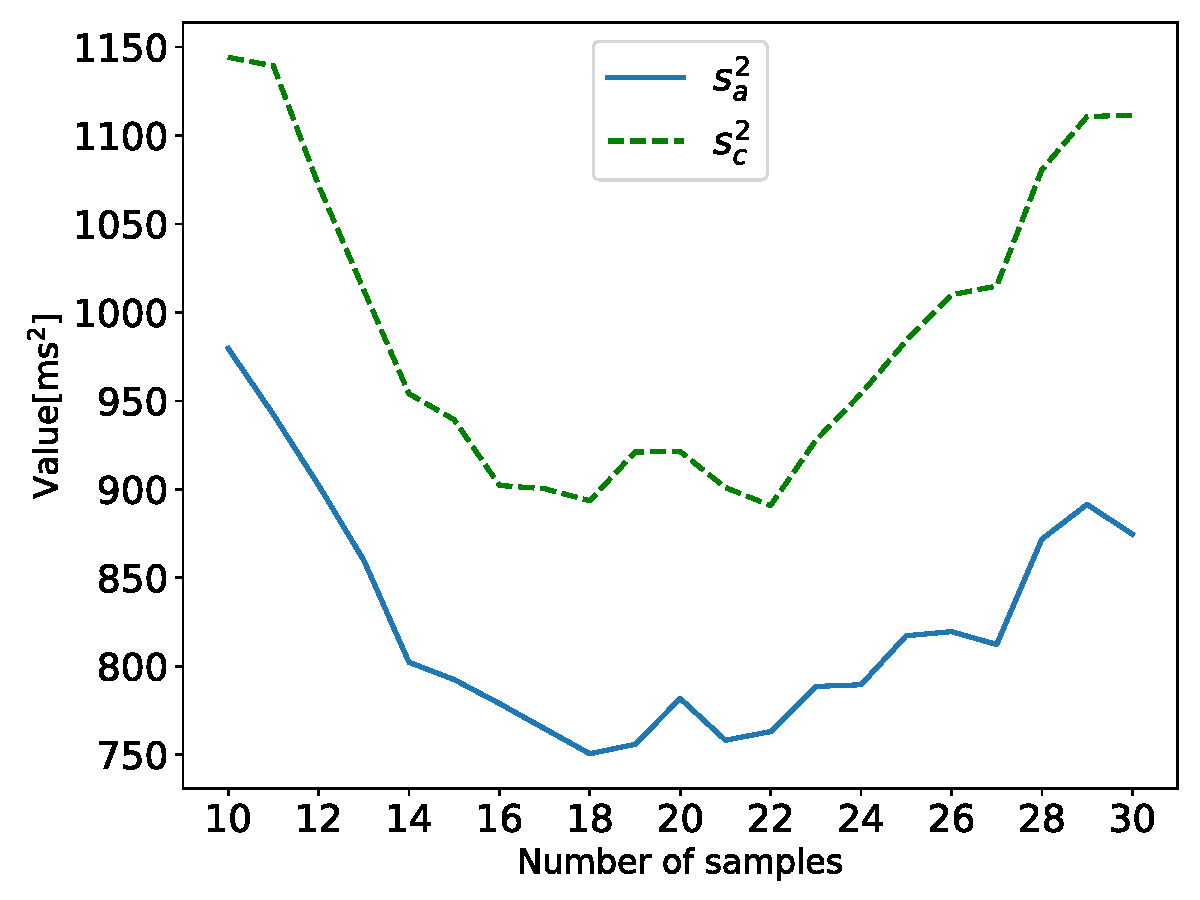
\includegraphics[scale=0.6]{figures/Yobi/Var/NumberOfSamples_varSaSc.pdf}
  \caption{使用するボタン押下時間間隔のデータの個数と評価指標の関係1}
  \label{fig:NumberofSamples_Sa_Sc}
\end{figure}
\begin{figure}[tbp]
  \centering
  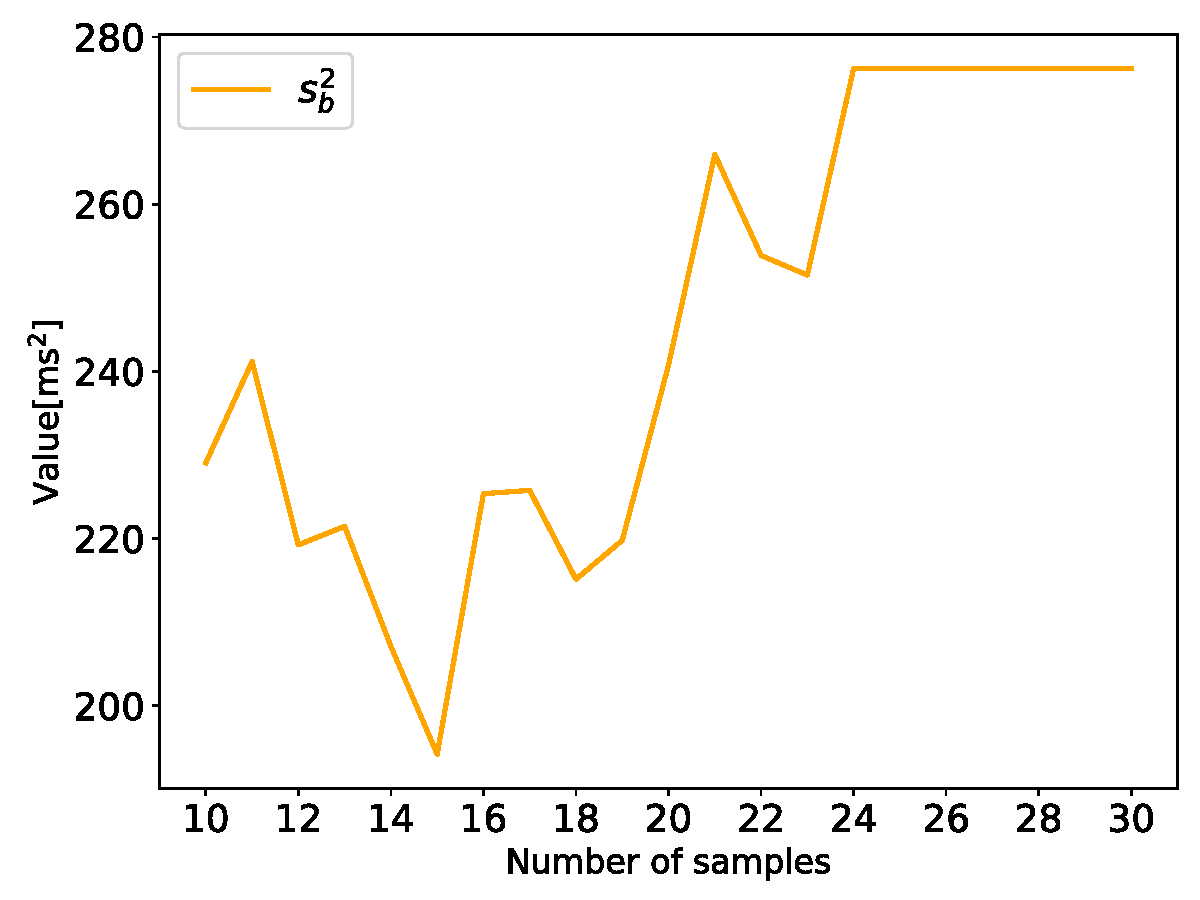
\includegraphics[scale=0.6]{figures/Yobi/Var/NumberOfSamples_varSb.pdf}
  \caption{使用するボタン押下時間間隔のデータの個数と評価指標の関係2}
  \label{fig:Numberofsamples_Sb}
\end{figure}

% \section{評価指標の値を算出する上での最適な条件}
% 先行研究[重松さんの論文]では,実験者が指定するボタンの押下回数を20回から10回間隔で40回までの3種類に変化させ,最も評価指標の値が小さくなるようなデータの開始点を算出した.本研究でも同様に評価指標の値が最も小さくなるようなデータの開始点を算出するために遅延を感じないとされている遅延時間10[ms]という条件でボタン押し課題を行い,本質的なばらつきが発生しないような最適な実験条件を探る.この実験では,ボタンの押下回数を40回に指定する.また,遅延時間を10[ms]に固定し行う.被験者は,20代の男女10名である.図6.2,図6.3に評価指標の時間変化を示す.また,図6.3に予備調査で遅延時間を変化させたときの結果の10msの時の結果を示す.被験者は,20人である.
% \newpage
% \begin{figure}[tb]
%   \centering
%   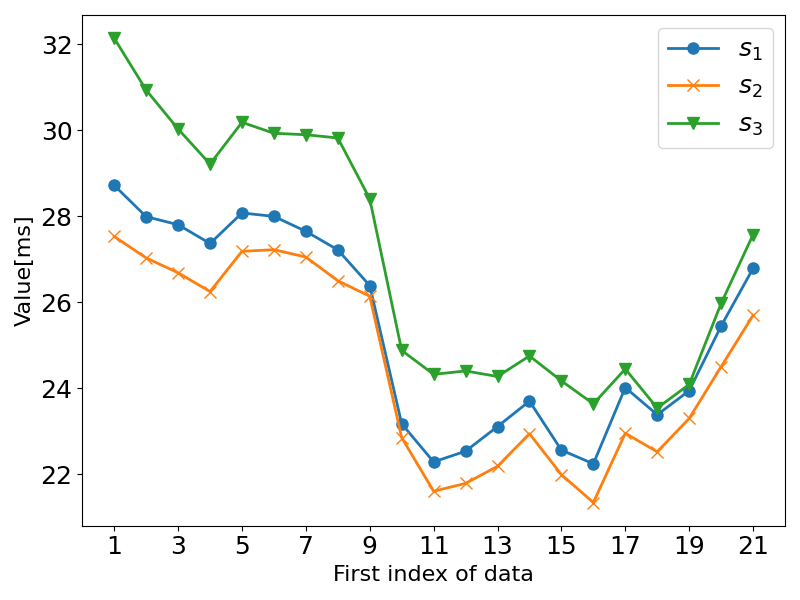
\includegraphics[scale=0.45]{figures/Yobi/Yobi_10ms_TimeChange.png}
%   \caption{評価指標の時間変化}
% \end{figure}
% \begin{figure}[tb]
%   \centering
%   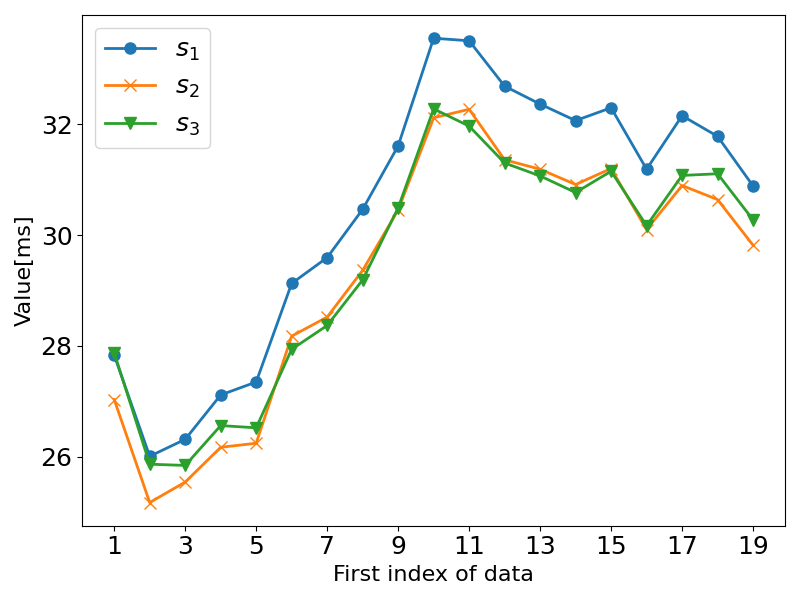
\includegraphics[scale=0.45]{figures/Yobi/Yobi_10ms_tyuuusyutu.png}
%   \caption{評価指標の時間変化}
% \end{figure}
% \newpage
\section{遅延を発生させる最適なタイミング}
本節では,6.1節で規定された適切なボタン押下時間間隔を用いて,遅延を発生させる最適なタイミングを検証する.
実験(1)では,被験者による予備調査後の口頭アンケート結果から,「遅延を感じなかった」あるいは「遅延を感じたが操作感に影響はなかった」との意見が寄せられた.
この結果を踏まえ,「ボタン押下時の合図音の遅延が一定であれば,被験者は遅延に適応し,ボタン押下の時間間隔に及ぼす影響が減少する」との仮説を立て,
「合図音の遅延が毎回でない場合,慣れの影響が軽減され,
遅延聴覚フィードバックの影響が明確に観察される」と考えた.
この仮説を検証するために,実験(2)では,ボタンの押下回数が4の倍数に達したときのみ遅延を発生させるシステムを用いて,
遅延聴覚フィードバックが身体運動に及ぼす影響を分析した.
\newpage
\begin{enumerate}[leftmargin=*, label=実験(\arabic*)]
    \item ボタンを押下したときの合図音が常に遅延する場合
    \item ボタンを押下するときの合図音がボタンの押下回数が4の倍数に達したときのみ遅延する場合
\end{enumerate}
上記2つの実験を行い,聴覚フィードバックの遅延時間とボタンの押下時間間隔のばらつきの関係が読み取り可能である実験条件を探る.
\subsection{調査方法}
若年者を対象に行った遅延聴覚フィードバックが身体運動に与える影響の調査方法を以下に示す.
実験(1)と実験(2)ともに調査の方法は同様である.
\begin{enumerate}[leftmargin=*]
  \item 被験者に図\ref{fig:button-click-system}のシステムを用意する.
  \item 4.1節で述べた手順1から手順2によって,ボタン押し課題を実施する.
  \item ヘッドホンから出力されるボタン押下の合図音の遅延時間をランダムに変更して実験者が指定した回数だけ手順2を繰り返す.
  このとき,実験者が提示する回数は,\ref{subsec:Yobi-conditions}項で提示する遅延時間の種類である.
  また,遅延時間を変更し,次の実験に移るときには20秒間の休憩を挟む.
\end{enumerate}
\subsection{調査条件および調査対象}
\label{subsec:Yobi-conditions}
先行研究\cite{kayama}においては,遅延聴覚フィードバックが発話に与える影響を若年者と高齢者に対して検証した.
その結果,90[ms]を超える遅延時間において,若年者と高齢者の間で遅延聴覚フィードバックに対する違和感に有意な差が見られた.
また,文献\cite{timing-music}では,遅延なしの状態と比較して100[ms]以上の遅延があるとリズムを刻む作業が困難になることが示されている.
これらを踏まえ,本研究では100[ms]未満の遅延時間においても身体運動に与える遅延聴覚フィードバックの影響を検証するため,
遅延時間を10, 30, 50, 70, 90, 110[ms]の6つに設定した.遅延時間の提示順序は,初めに10[ms]を提示し,次に10[ms]以外の中からランダムに選択し提示する.
その後,残る遅延時間に10[ms]を加えたものをランダムに提示する.
遅延時間が10[ms]の時の評価値の算出については,最初に提示したものではなくランダムに提示したものの結果を用いる.
表\ref{table:A_delay_time}に実験(1)における遅延時間の提示順序,被験者数および被験者の年齢の平均と年齢の最小値および最大値を示し,
表\ref{table:B_delay_time}に実験(2)における同様の情報を示す.
調査結果は,実験(1)では,提示する遅延時間ごとに5.1節の$s^2_{a}$,$s^2_{b}$および$s^2_{c}$を算出し,
実験(2)では,提示する遅延時間ごとに5.1節の$s^2_{a}$,$s^2_{b}$および$s^2_{c}$と5.2節で述べたMSEおよびMedSEを算出することで評価した.
\begin{table}[tbp]
  \caption{実験(1)における遅延時間の提示順}
  \label{table:A_delay_time}
  \centering
  \begin{tabular}{lccc}
    \hline
    提示順 & 遅延時間 & 被験者数 & 年齢\\
     & [ms] & & $\bigl(平均 (最小-最大)\bigr)$\\
    \hline \hline
    提示順1  & 10, 30, 110, 10, 70, 90, 50  & 3 & $22.0\, (21-23)$\\
    提示順2  & 10, 70, 30, 110, 50, 90, 10  & 5 & $22.4\, (22-23)$\\
    提示順3  & 10, 110, 90, 50, 10, 30, 70  & 4 & $23.0\, (22-24)$\\
    提示順4  & 10, 50, 90, 10, 30, 70, 110  & 4 & $22.5\, (22-24)$\\
    提示順5  & 10, 30, 10, 50, 110, 70, 90  & 5 & $21.8\, (21-22)$
\\
    \hline
  \end{tabular}
\end{table}

\begin{table}[tbp]
  \caption{実験(2)における遅延時間の提示順}
  \label{table:B_delay_time}
  \centering
  \begin{tabular}{lccc}
    \hline
    提示順 & 遅延時間 & 被験者数 & 年齢\\
     & [ms] & & $\bigl(平均 (最小-最大)\bigr)$\\
    \hline \hline
    提示順1  & 10, 30, 110, 10, 70, 90, 50  & 4 & $22.5\, (22-24)$\\
    提示順2  & 10, 70, 30, 110, 50, 90, 10  & 3 & $22.0\, (22-22)$\\
    提示順3  & 10, 110, 90, 50, 10, 30, 70  & 3 & $23.7\, (22-25)$\\
    提示順4  & 10, 50, 90, 10, 30, 70, 110  & 3 & $21.7\, (21-22)$\\
    提示順5  & 10, 30, 10, 50, 110, 70, 90  & 3 & $22.7\, (21-25)$
\\
    \hline
  \end{tabular}
\end{table}
\subsection{調査結果}
\begin{figure}[tbp]
  \centering
  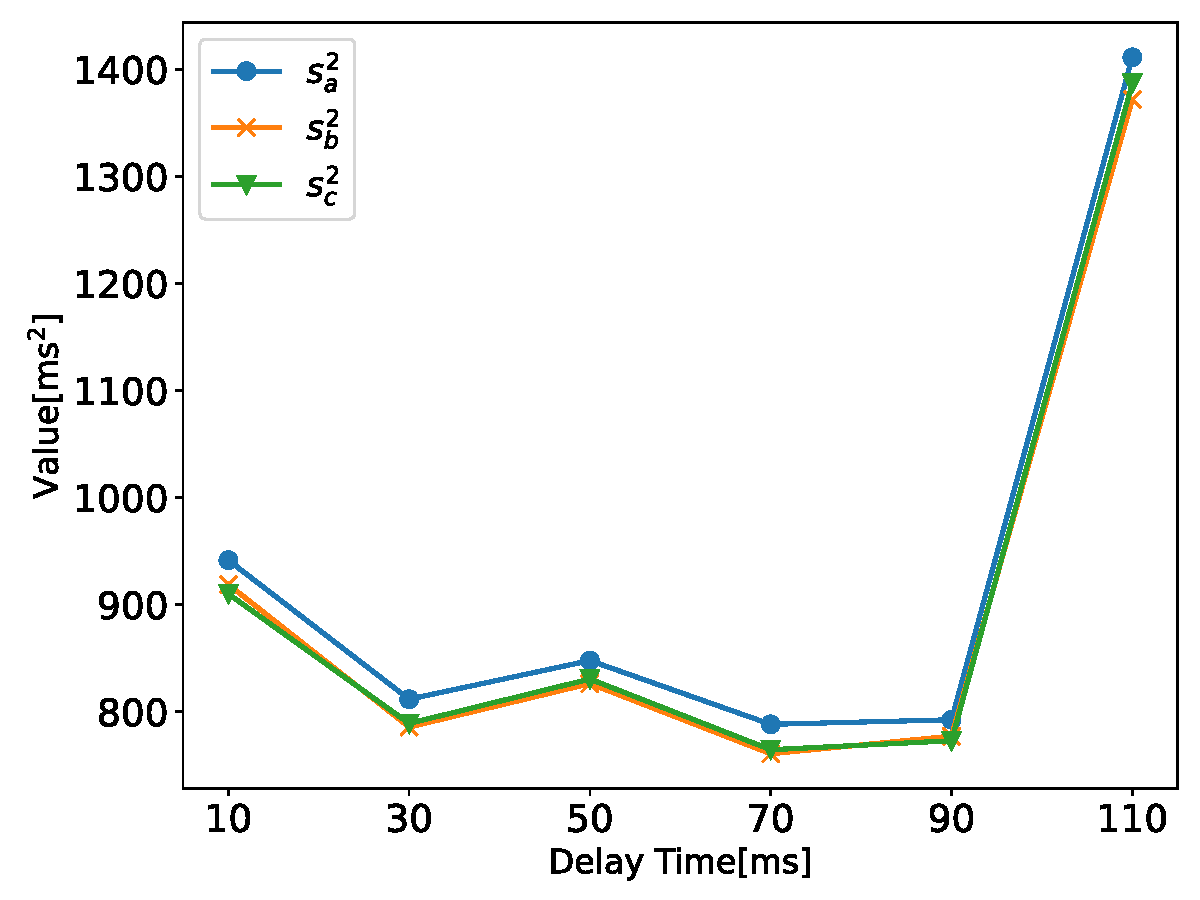
\includegraphics[scale=0.5]{figures/Yobi/Var/Var-Normal.pdf}
  \caption{実験(1)における遅延時間と評価指標の関係}
  \label{fig:Normal_bunsan}
\end{figure}
\begin{figure}[bt]
  \centering
  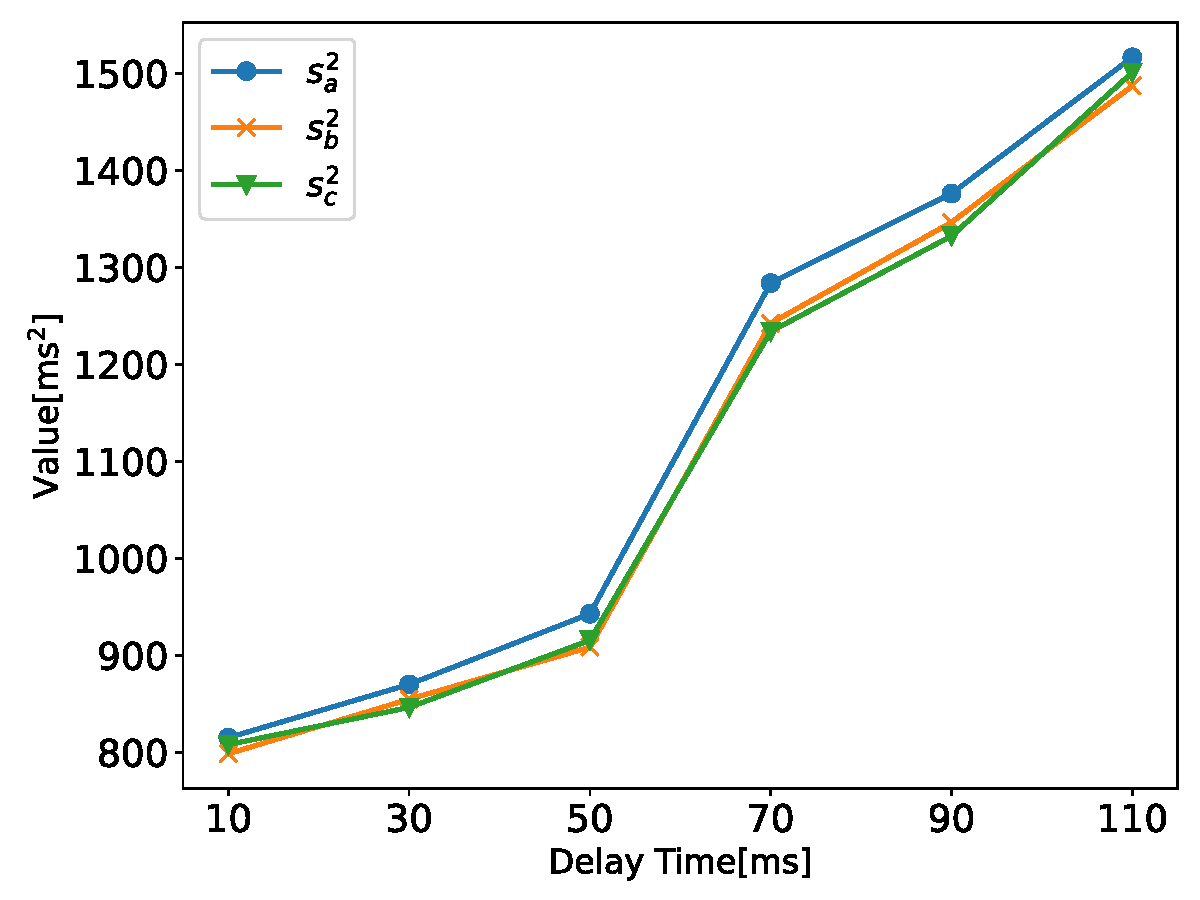
\includegraphics[scale=0.5]{figures/Yobi/Var/Var-Yobi-Unique.pdf}
  \caption{実験(2)における遅延時間と評価指標の関係}
  \label{fig:Unique_bunsan}
\end{figure}
\begin{figure}[bt]
  \centering
  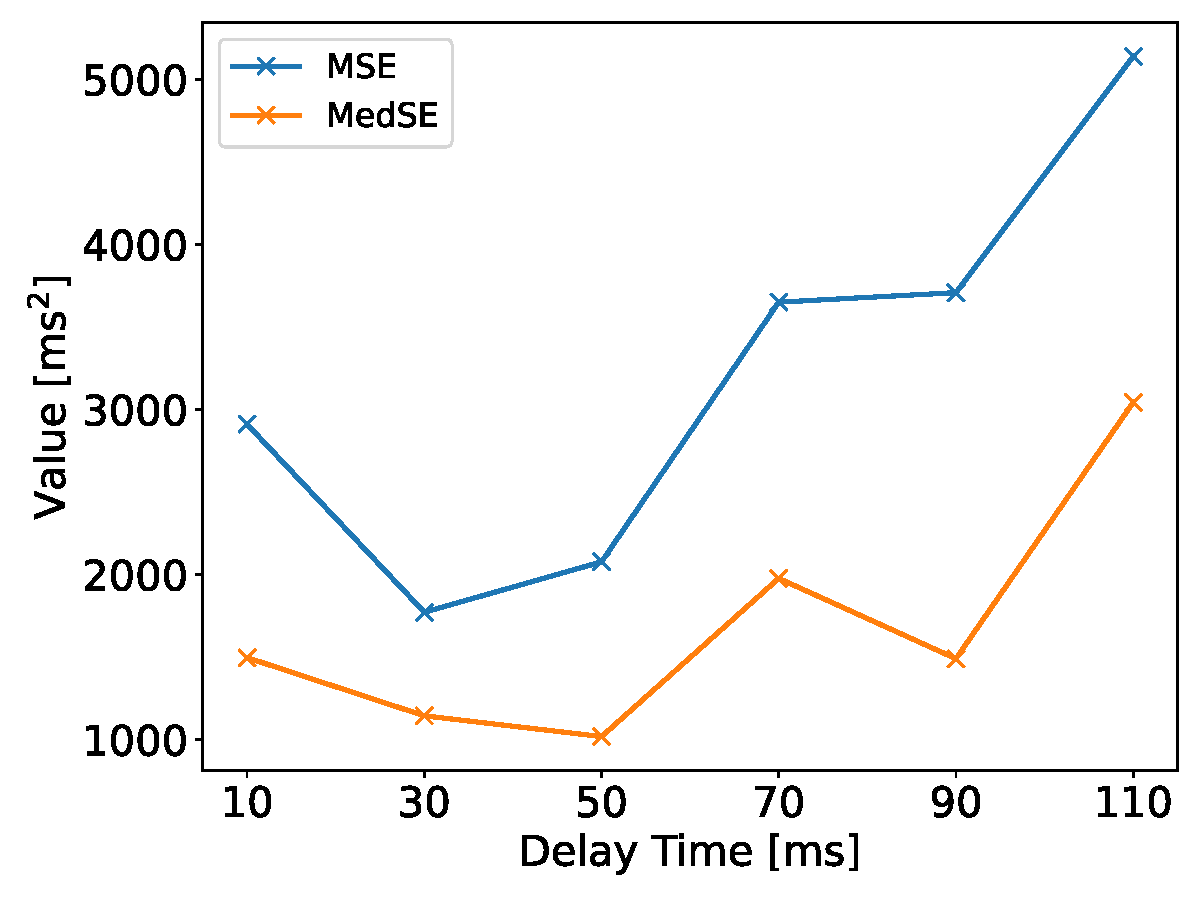
\includegraphics[scale=0.5]{figures/Yobi/Var/Yobi-MSE-MedSE.pdf}
  \caption{実験(2)における遅延時間とMSEおよびMedSEの関係}
  \label{fig:Yobi_MSE_MedSE}
\end{figure}
図\ref{fig:Normal_bunsan}に実験(1)による遅延聴覚フィードバックの身体運動への影響の調査結果を,
図\ref{fig:Unique_bunsan}に実験(2)における同様の影響の調査結果を,図\ref{fig:Yobi_MSE_MedSE}に実験(2)における遅延時間とMSEおよびMedSEの関係を示す.
図\ref{fig:Normal_bunsan}に示される結果から,10[ms]から90[ms]の間で評価指標が減少する傾向が見られ,
90[ms]から110[ms]の範囲では評価指標が急激に増加していることが観察される.
10[ms]から90[ms]の間での評価指標の減少は,被験者が遅延に馴化した結果である可能性が高い.
これは,一貫した遅延を持つシステムにおいて,繰り返されるボタン押し課題を通じて被験者が遅延に順応し,
より大きな遅延にも対応できるようになることを示唆している.
一方,図\ref{fig:Unique_bunsan}の実験(2)の結果では,10[ms]の評価値が最小であり,
遅延時間の増加に伴い評価値が上昇する傾向が確認できる.
さらに,図\ref{fig:Yobi_MSE_MedSE}では,10[ms]から30[ms]の間で評価値が減少しているものの,
30[ms]から110[ms]にかけて評価値が増加する傾向が見られる.
これは,不規則な遅延が身体運動に与える影響を示しており,4回に1度の遅延が特に影響を及ぼしている可能性がある.
これらの結果から,遅延が一定である場合,被験者はその遅延に馴染み,ボタン押下時間間隔に及ぼす影響が減少する
という仮説を支持する.
したがって,本研究では次回以降の実験を実験(2)の条件で進めることにする.
これにより,遅延聴覚フィードバックが身体運動に与える影響のより詳細な理解を目指す.

% コメントアウト
% \begin{figure}[bt]
%   \centering
%   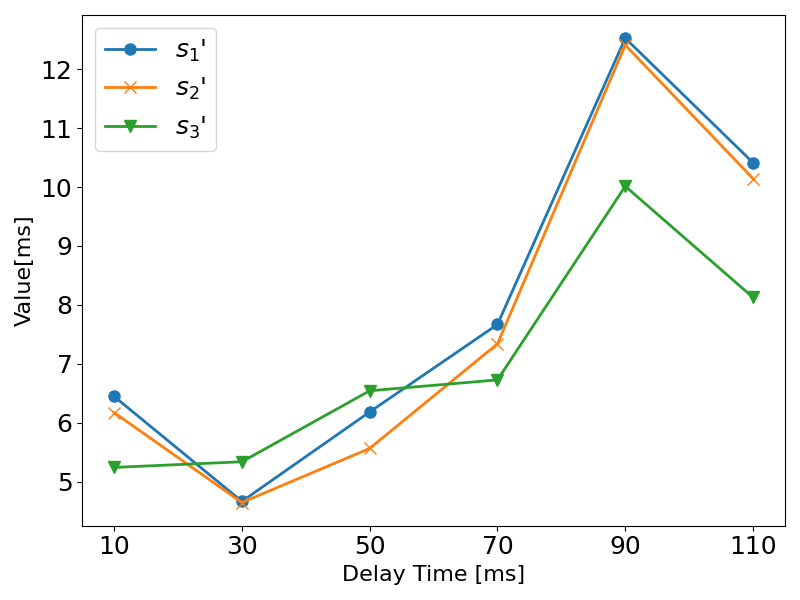
\includegraphics[scale=0.5]{figures/Yobi/Yobi_2And2_110ms.png}
%   \caption{直前と直後2回ずつ}
% \end{figure}
\newpage \newpage
% \section{遅延への順応の示唆}
% 文献[重松さんの修論]では,分析するデータの開始点によって,評価値の値が変化すると報告されている.そこで,本節でも,6.3節の結果から示唆された遅延への順応について,分析対象のデータの開始点を様々に変化させることによって,遅延への順応の可能性を検証し,今後の調査に役立てる.

\chapter{遅延聴覚フィードバックが身体運動に与える影響の調査}
本章では,第4章で開発されたシステムと第6章で決定された実験条件を用いて,遅延聴覚フィードバックが身体運動に及ぼす影響を聴力が正常な若年者および60代以上の高齢者に対して調査した結果について述べる.
「高齢者は若年者に比べて聴覚フィードバックの遅延に対する許容度が高い」という仮説を,4の倍数に達したときのみ遅延を発生させるシステムを用いて検証する.
第6章の予備実験により,4の倍数に達する直前の押下間隔と4の倍数に達した直後の押下間隔の差の二乗の平均値および中央値が遅延時間の増加に比例して増大すること,そして4の倍数に達したときの遅延が全体のボタン押下間隔のばらつきを拡大させるという可能性が示唆された.
これらの予備実験で得られた考察を基に,仮説の検証を行う.
\section{調査方法}
聴力の正常な若年者および高齢者を対象に行ったボタン押し課題による遅延聴覚フィードバックが身体運動に与える影響の調査の方法を以下に示す.
\begin{enumerate}
  \item 被験者に図4.1のシステムを用意する.
  \item 4章の手順1から手順2までに述べた方法によって,ボタン押し課題を実施する.
  \item ヘッドホンから出力される音声の遅延時間をランダムに変更して実験者がアプリケーション上で指定した回数だけ手順2を繰り返す.
  このとき,実験者が提示する回数は,7.2節で提示する遅延時間の種類によって異なる.
\end{enumerate}
\section{調査条件および調査対象}
遅延時間の提示順序は,最初に10[ms]を提示し,次に10[ms]以外の中からランダムに選択し提示する.
その後,残る遅延時間に10[ms]を加えたものをランダムに提示する.
提示する遅延時間の種類を表\ref{table:young_a},表\ref{table:young_b},表\ref{table:old_a}および表\ref{table:old_b}に示す.
本研究では,10, 30, 50, 70, 90, 110[ms]の6種類の遅延時間を用いた実験を実験Aとし,
10, 15, 20, 25, 35, 30, 40[ms]の7種類の遅延時間を用いた実験を実験Bと称する.
\begin{table}[tbp]
  \caption{若年者の実験Aにおける遅延時間の提示順}
  \label{table:young_a}
  \centering
  \begin{tabular}{lccc}
    \hline
    提示順 & 遅延時間 & 被験者数 & 年齢\\
     & [ms] & & $\bigl(平均 (最小-最大)\bigr)$\\
    \hline \hline
    提示順1  & 10, 30, 110, 10, 70, 90, 50  & 8 & $22.1\, (21-23)$\\
    提示順2  & 10, 70, 30, 110, 50, 90, 10  & 8 & $22.4\, (21-24)$\\
    提示順3  & 10, 110, 90, 50, 10, 30, 70  & 8 & $22.3\, (21-25)$\\
    提示順4  & 10, 50, 90, 10, 30, 70, 110  & 7 & $22.7\, (22-24)$\\
    提示順5  & 10, 30, 10, 50, 110, 70, 90  & 7 & $23.1\, (22-24)$
\\
    \hline
  \end{tabular}
\end{table}
\begin{table}[tbp]
  \caption{若年者の実験Bにおける遅延時間の提示順}
  \label{table:young_b}
  \centering
  \begin{tabular}{lccc}
    \hline
    提示順 & 遅延時間 & 被験者数 & 年齢\\
     & [ms] & & $\bigl(平均 (最小-最大)\bigr)$\\
    \hline \hline
    提示順1  & 10, 25, 35, 30, 40, 20, 10, 15  & 7 & $22.6\,(21-24)$\\
    提示順2  & 10, 15, 40, 10, 35, 25, 30, 20  & 7 & $22.9\,(21-25)$\\
    提示順3  & 10, 30, 25, 10, 40, 20, 35, 15  & 7 & $22.6\,(21-25)$\\
    提示順4  & 10, 30, 20, 10, 15, 35, 25, 40  & 7 & $22.1\,(20-24)$\\
    提示順5  & 10, 40, 10, 25, 30, 20, 15, 35  & 6 & $23.5\,(22-24)$
\\
    \hline
  \end{tabular}
\end{table}
\begin{table}[btp]
  \caption{高齢者の実験Aにおける遅延時間の提示順}
  \label{table:old_a}
  \centering
  \begin{tabular}{lccc}
    \hline
    提示順 & 遅延時間 & 被験者数 & 年齢\\
     & [ms] & & $\bigl(平均 (最小-最大)\bigr)$\\
    \hline \hline
    提示順1  & 10, 30, 110, 10, 70, 90, 50  & 8 & $63.5\, (60-70)$\\
    提示順2  & 10, 70, 30, 110, 50, 90, 10  & 8 & $70.1\, (61-77)$\\
    提示順3  & 10, 110, 90, 50, 10, 30, 70  & 8 & $68.4\, (63-77)$\\
    提示順4  & 10, 50, 90, 10, 30, 70, 110  & 9 & $70.2\, (61-82)$\\
    提示順5  & 10, 30, 10, 50, 110, 70, 90  & 8 & $74.1\, (68-83)$
\\
    \hline
  \end{tabular}
\end{table}
\begin{table}[btp]
  \caption{高齢者の実験Bにおける遅延時間の提示順}
  \label{table:old_b}
  \centering
  \begin{tabular}{lccc}
    \hline
    提示順 & 遅延時間 & 被験者数 & 年齢\\
     & [ms] & & $\bigl(平均 (最小-最大)\bigr)$\\
    \hline \hline
    提示順1  & 10, 25, 35, 30, 40, 20, 10, 15  & 8 & $70.0\,(60-80)$\\
    提示順2  & 10, 15, 40, 10, 35, 25, 30, 20  & 8 & $72.1\,(60-90)$\\
    提示順3  & 10, 30, 25, 10, 40, 20, 35, 15  & 8 & $67.9\,(60-88)$\\
    提示順4  & 10, 30, 20, 10, 15, 35, 25, 40  & 9 & $75.2\,(62-84)$\\
    提示順5  & 10, 40, 10, 25, 30, 20, 15, 35  & 8 & $73.1\,(65-80)$
\\
    \hline
  \end{tabular}
\end{table}
\newpage
\section{調査結果}
\subsection{観測値の分布}
% データの代表的な統計量,特に平均や標準偏差は,対象のデータ分布が正規分布に従っている場合にその真の特性を正確に反映する.
% したがって,遅延時間ごとに得られたボタンの押下時間間隔のデータが正規分布に従うかどうかを確認することが必要である.
% これにより,分散や標準偏差を用いてデータ分布のばらつきを評価することの妥当性を検討する.
% 帰無仮説を「ボタン押下時間間隔のデータの母集団の分布は,正規分布に従う」として,コルモゴロフ・スミルノフ検定を用いて,有意水準5%で観測値が正規分布に従うかどうかを検定する.
% 遅延時間に応じたボタンの押下時間間隔のデータのヒストグラムを図7.1,図7.2,図7.3,図7.4に示す.また,正規性の検定の結果を表7.1に記載する.
% 外れ値の除去は,被験者ごとに各遅延時間での観測値を
本節では,遅延時間ごとに得られたボタンの押下時間間隔のデータの分布を箱ひげ図を用いて示す.
箱ひげ図は,観測値の中央値,第1四分位数,第3四分位数を示すことで,データの分布状況および中心的傾向を効果的に視覚化する.
加えて,箱ひげ図に外れ値を示すことで,データのばらつきを直接的に評価することが可能となる.外れ値の算出は,以下の手順により行う.
\begin{enumerate}
  \item 各遅延時間におけるボタンの押下時間間隔のデータを,被験者ごとに集計する.
  \item 各遅延時間でのボタンの押下時間間隔のデータの中央値,第1四分位数,第3四分位数を算出する.
  \item 第3四分位数から第1四分位数を引いた値である四分位範囲(Interquartile Range, IQR)を計算する.
  \item (3)で求めたIQRを1.5倍し,この値を第三四分位数に加算および第一四分位数から減算した結果を上下の閾値と定める.
  \item 閾値内の最も遠いデータまで箱からひげを引く.
  \item 各データと閾値を比較し,4で求めた閾値の外にある値を全て外れ値とし,点で表す.
\end{enumerate}
これにより,データの基本的な統計的特徴を簡潔に表現し,後続の分析におけるデータの解釈を支援する.
図\ref{fig:110ms_Distribution_of_observations},図\ref{fig:40ms_Distribution_of_observations},
図\ref{fig:110ms_Distribution_of_observations_by_old}および図\ref{fig:40ms_Distribution_of_observations_by_old}に遅延時間ごとのボタンの押下時間間隔のデータの分布を示す.
これらの図より,それぞれの遅延時間でのボタンの押下時間間隔のデータには,一定数の外れ値が存在することがわかる.
したがって,本研究では外れ値を除外したデータを用いて分析を行う.
この方法により,これから行う分析において,外れ値の影響を排除し,適切な評価を行うためのデータを用いることができる.

\begin{figure}[tbp]
  \centering
  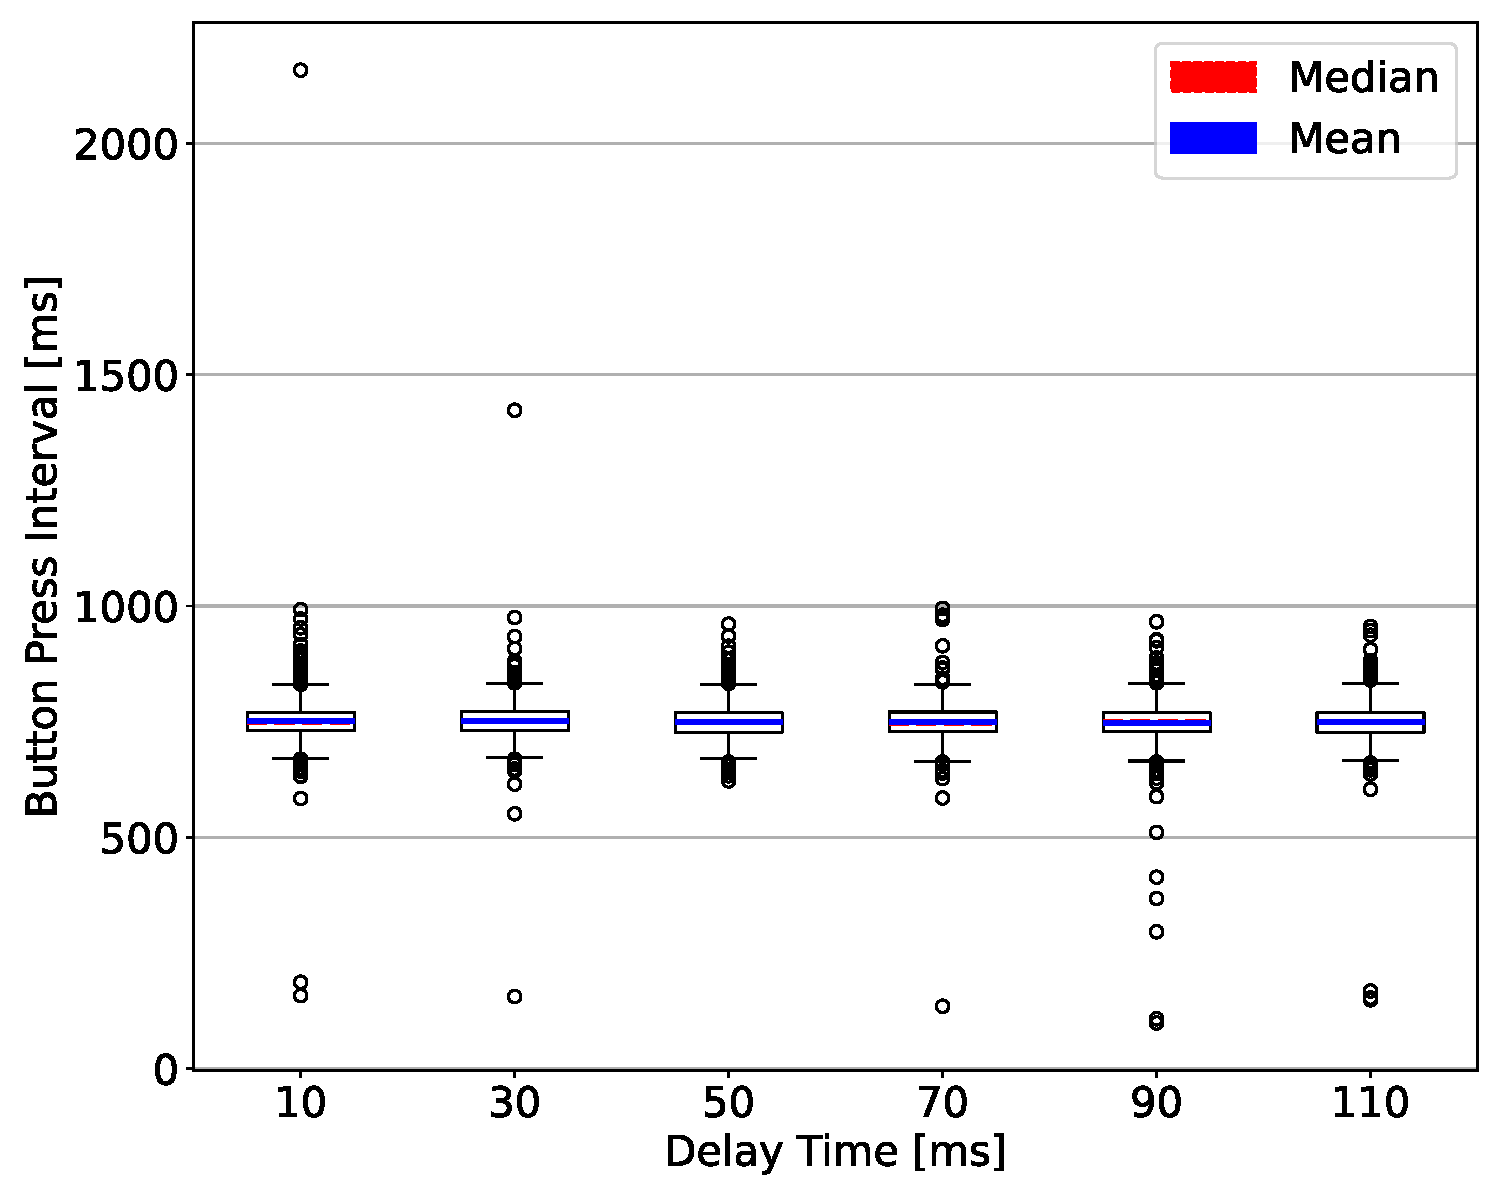
\includegraphics[scale=0.4]{figures/Honbann/BOXPLOT/young_110_boxplot.pdf}
  \caption{実験Aにおける遅延時間ごとの若年者のデータの分布}
  \label{fig:110ms_Distribution_of_observations}
\end{figure}
\begin{figure}[tbp]
  \centering
  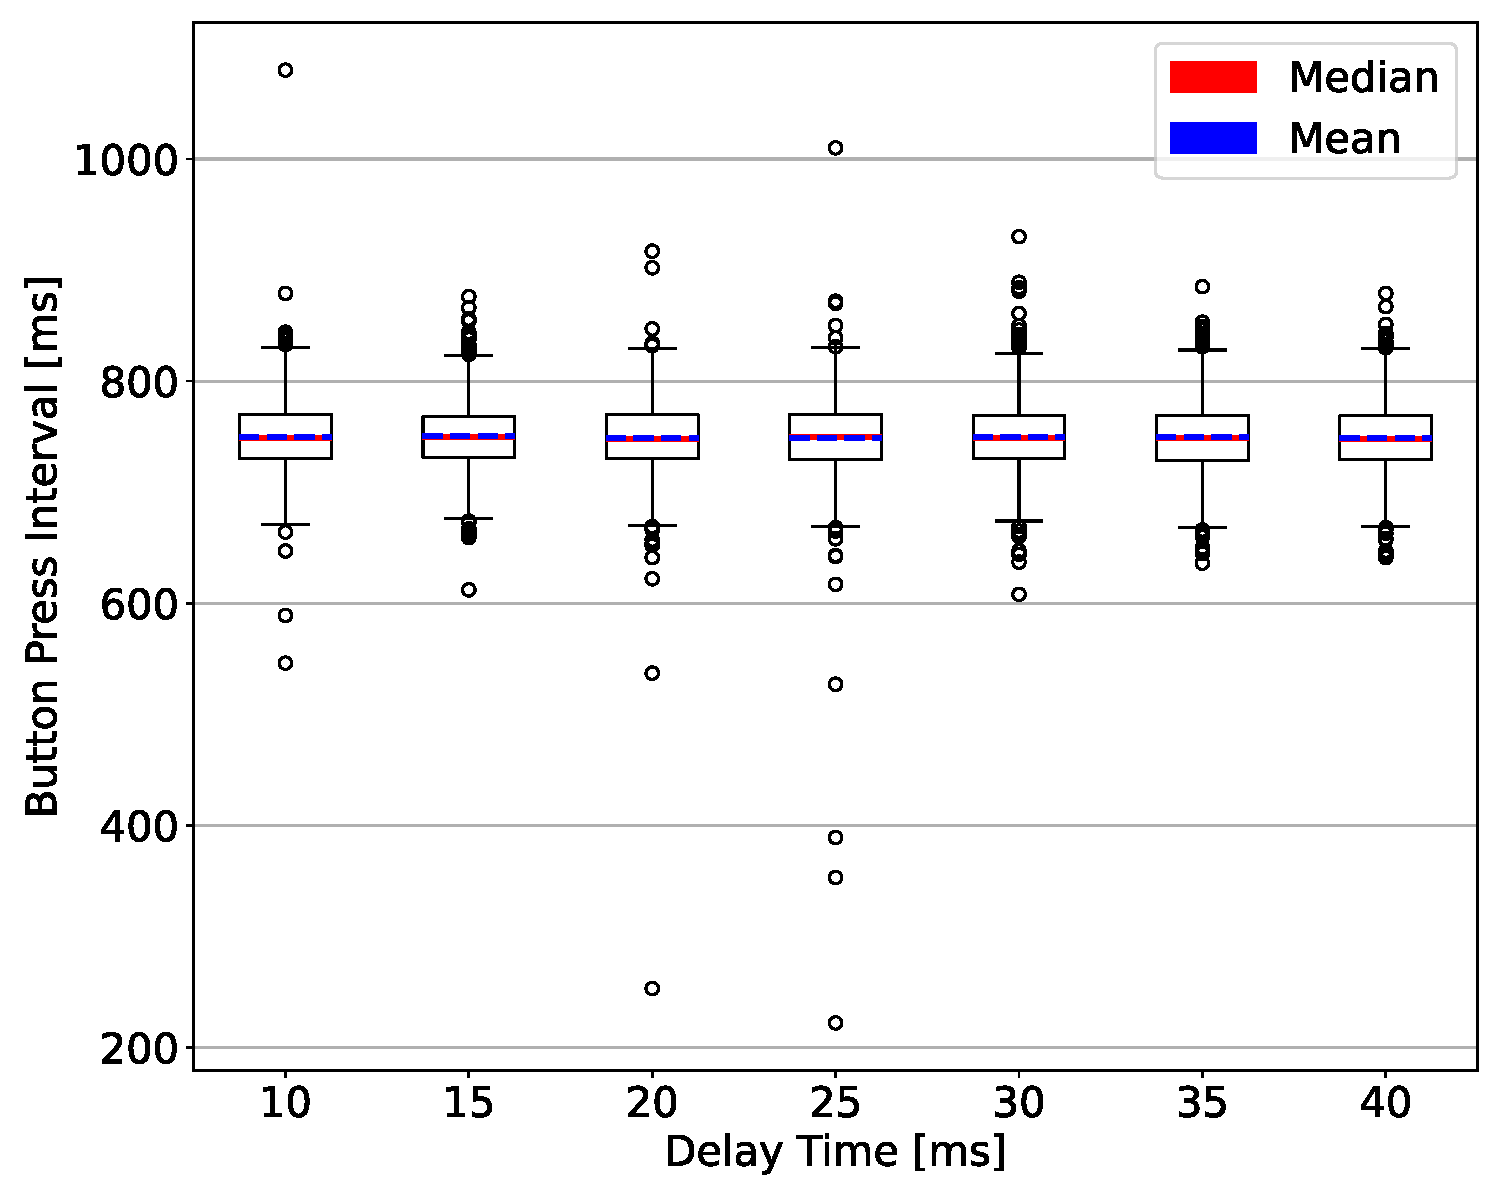
\includegraphics[scale=0.4]{figures/Honbann/BOXPLOT/young_40_boxplot.pdf}
  \caption{実験Bにおける遅延時間ごとの若年者のデータの分布}
  \label{fig:40ms_Distribution_of_observations}
\end{figure}
\begin{figure}[tbp]
  \centering
  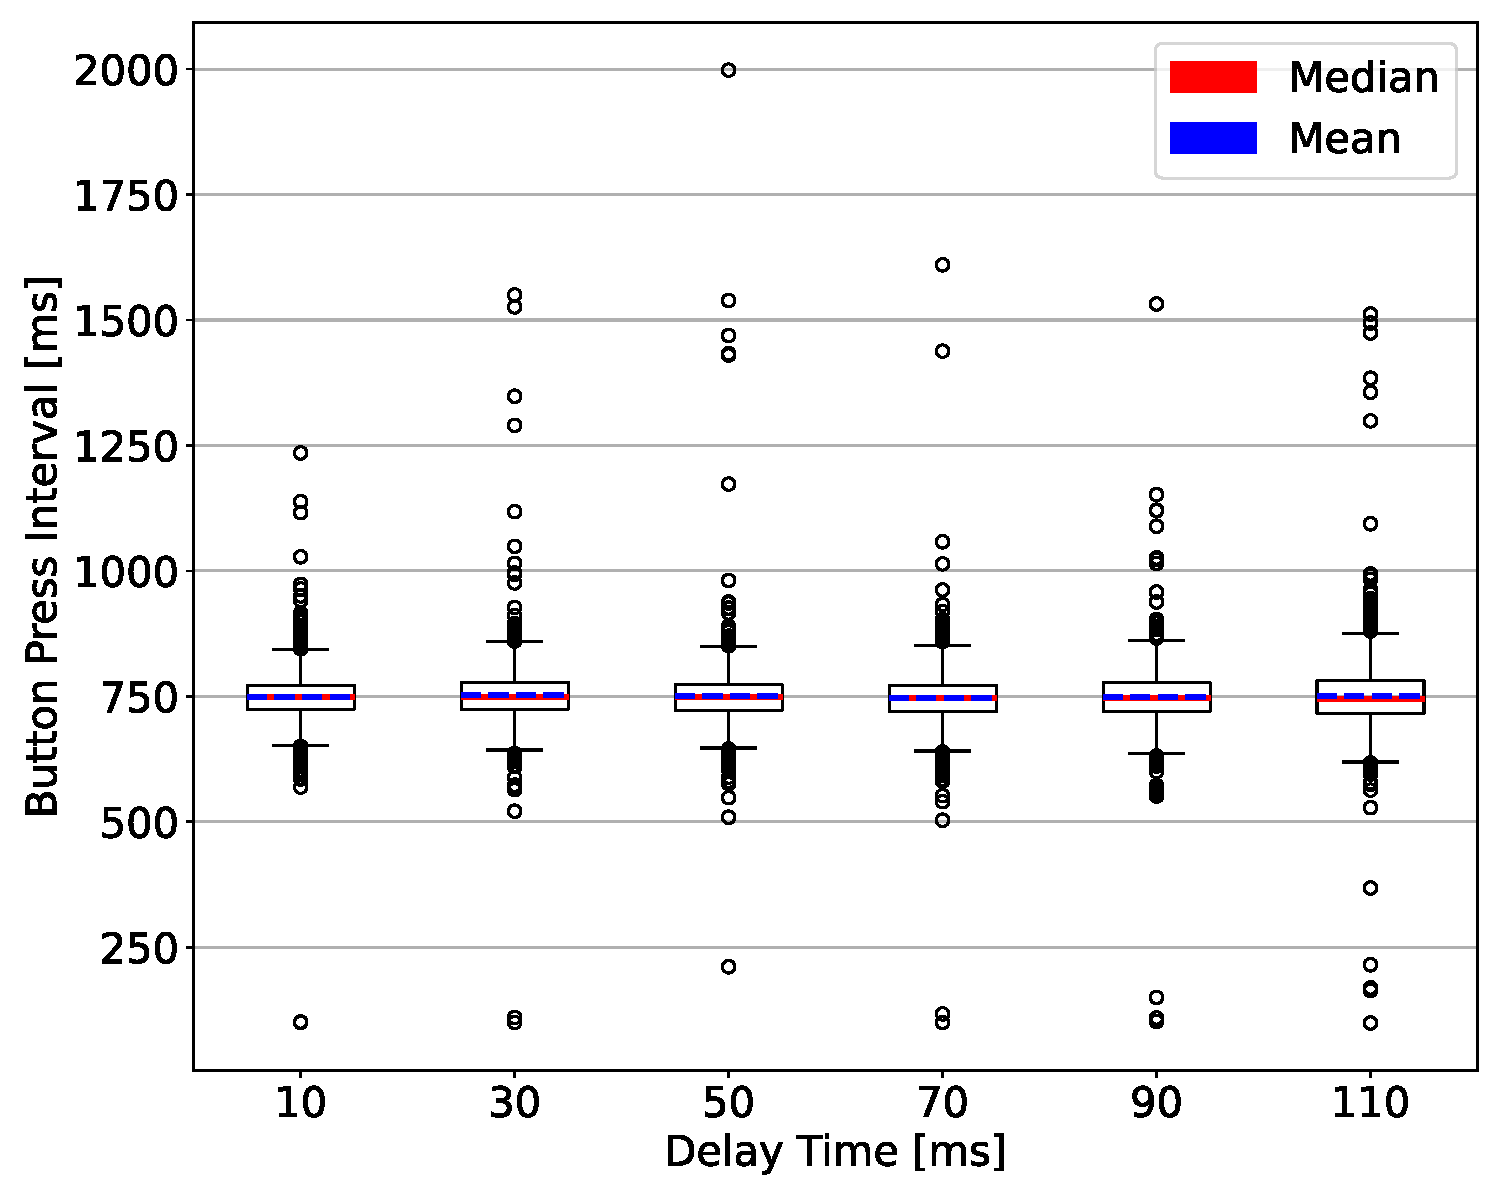
\includegraphics[scale=0.4]{figures/Honbann/BOXPLOT/old_110_boxplot.pdf}
  \caption{実験Aにおける遅延時間ごとの高齢者のデータの分布}
  \label{fig:110ms_Distribution_of_observations_by_old}
\end{figure}
\begin{figure}[tbp]
  \centering
  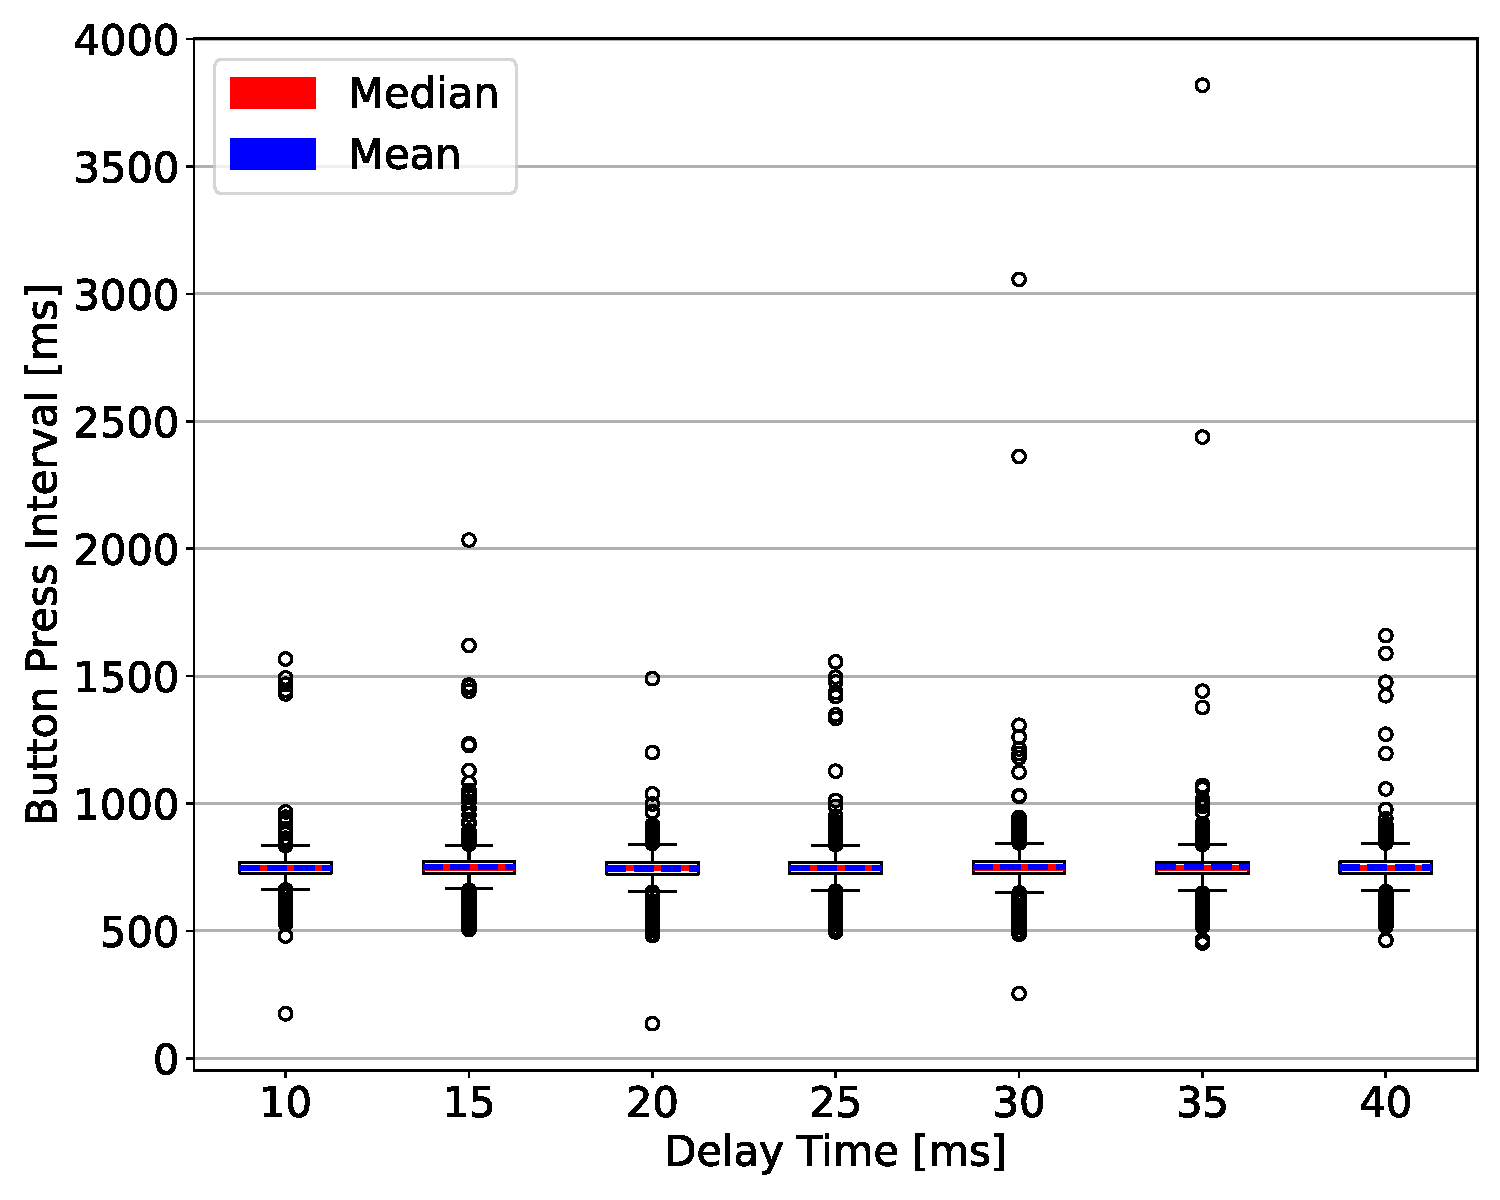
\includegraphics[scale=0.4]{figures/Honbann/BOXPLOT/old_40_boxplot.pdf}
  \caption{実験Bにおける遅延時間ごとの高齢者のデータの分布}
  \label{fig:40ms_Distribution_of_observations_by_old}
\end{figure}
\newpage
% 結果の考察
\subsection{遅延時間と評価指標の関係}
本節では,7.3.1項で説明した方法によりデータの外れ値を除去した後の遅延聴覚フィードバックが身体運動に与える影響の調査結果を標本全体の分散,
遅延直前後の押下間隔の差の二乗の平均値(Mean Squared Error, MSE),遅延直前後の押下間隔の差の中央値(Median Squared Error, MedSE)
の3つの評価指標を用いて示す.
遅延時間と評価値の関係が若年者と高齢者で異なるかどうかを検証するために,若年者と高齢者それぞれの結果を同一グラフ上に表示し,比較する.
図\ref{fig:Var_110ms_Sa_Sb},図\ref{fig:Var_110ms_Sc}に実験Aにおける遅延時間と分散の関係,
図\ref{fig:Var_40ms_Sa_Sb},図\ref{fig:Var_40ms_Sc}に実験Bにおける遅延時間と分散の関係,
図\ref{fig:Normalized-Var_110ms_SaSbSc},図\ref{fig:Normalized-Var_40ms_SaSbSc}に実験A,実験Bにおける遅延時間と分散の関係において,10ms時の評価値を基準に正規化した場合の結果を示す.
図\ref{fig:110ms_MSE_MedSE},図\ref{fig:Normalized_110ms_MSE_MedSE}にMSEおよびMedSEの結果を,
図\ref{fig:40ms_MSE_MedSE},図\ref{fig:Normalized_40ms_MSE_MedSE}にMSEおよびMedSEの結果を10ms時の評価値で正規化した場合の結果を示す.

%%%%%%%%%%%%%%%%%%%%%%%%%%%%%%%
% 実験A
%%%%%%%%%%%%%%%%%%%%%%%%%%%%%%%
はじめに,実験Aにおける結果について述べる.
実験Aの結果において,ボタンの押下時間間隔全体の分散を評価値とする指標によれば,正規化されたデータでは若年者と高齢者の反応に顕著な差異が見られる.
若年者は,一貫して評価値が緩やかに増加するのに対し,高齢者は110[ms]を境に分散が大幅に増加することが示された.
また,実験AにおけるMSEおよびMedSEによる評価からも,遅延時間の増加に伴い,若年者と高齢者双方の評価値に増加の傾向が確認された.
この結果は,ボタン押し課題で提供される聴覚フィードバックの遅延が長くなるにつれて,遅延聴覚フィードバックの影響がより顕著になることを示唆している.
若年者は遅延時間の増加に対して比較的均一な反応を示したが,対照的に高齢者は70[ms]まで比較的緩やかな増加を見せた後,90[ms], 110[ms]の遅延時間において顕著な反応の増加を示した.
これは,高齢者がある程度の遅延には許容度を持つことを示唆しており,遅延時間が110[ms]に達した際には,若年者との差異が特に明確になった.
これらの結果から,高齢者が若年者と比較して聴覚フィードバックの遅延に対する許容度が高い可能性が示され,結果として遅延時間の増加に対する高齢者の感知の鈍さが推測される.
さらに,高齢者の評価値が若年者と比較して一貫性に欠けることからも,高齢者が遅延に対して鈍感である可能性も示唆される.

%%%%%%%%%%%%%%%%%%%%%%%%%%%%%%%
% 実験B
%%%%%%%%%%%%%%%%%%%%%%%%%%%%%%
次に,実験Bにおける結果について述べる.
実験Bにおいてもボタン押し課題の押下時間間隔全体の分散を通じて分析した結果,若年者と高齢者での間で異なる傾向が観察された.
正規化されたデータに基づく評価では,10[ms]から40[ms]の遅延時間帯において,若年者の分散は一貫して低い水準を維持しながらも緩やかに増加しているのに対し,
高齢者は遅延時間と評価値の間に一貫した関係が認められない.
% このことは,若年者が遅延時間の増加に対して一貫性を維持しやすく,高齢者は,遅延時間の増加に対して一貫性を維持することが困難であることを示唆している.
非正規化されたデータに基づく分析でも,高齢者は遅延時間に対して比較的一貫した分散の値を示しているが,若年者に比べて全体的に高い分散値を記録している.
これらのことは,高齢者が遅延時間の増加に対して若年者よりも鈍感であることを示唆し,逆に若年者が遅延時間の変化に対してより敏感である可能性を示している.
また,MSEおよびMedSEによる評価では,10[ms]から40[ms]の比較的短い遅延時間帯において,若年者における評価値が緩やかに増加する傾向が認められ,
若年者が遅延時間の増加に対して比較的敏感であること,そして遅延聴覚フィードバックによる影響をより感じやすいことを示唆している.
一方で,高齢者においては,遅延時間と評価値の間に一貫した関係が見出されず,遅延に対する感受性の低さが示唆される.
% 特に,高齢者群の評価値は遅延時間の変化に対して一定のばらつきを示しており,これは高齢者が遅延に対して鈍感である可能性を示している.

%%%%%%%%
% 結び
%%%%%%%%
以上の結果をまとめると,10[ms]から40[ms]の短い遅延時間帯における観察結果から,若年者の反応は遅延時間の増加に伴い緩やかに増加する傾向にあるが,
高齢者の反応には一貫した関係が認められないことが示された.このことは,若年者が遅延に対して敏感であり,一方で高齢者が遅延時間に対してある程度の
許容度を持っていることを示唆している.
一方,遅延時間を10[ms]から110[ms]に拡大した場合,特に90[ms]を超える長い遅延時間帯における高齢者の反応に大幅な増加が観察され,高齢者が遅延時間の
増加に対して比較的鈍感であるものの,90[ms]を超えるとタスクの一貫性を保つことが困難になることが示された.
若年者も長い遅延時間において,反応の増加を示したが,この増加は高齢者ほど急激ではなかった.
これらの結果は,遅延時間が増加するにつれて若年者と高齢者の反応の差異が顕著になることを示し,
若年者は短い遅延時間帯でも遅延を感じやすく,高齢者は長い遅延時間において特に顕著な反応を示したことを明らかにする.
さらに,遅延時間に対する年齢別の感受性の違いは,遅延聴覚フィードバックにおける効果を最大化するための異なるアプローチの
重要性を協調するものと思われる.
% 高齢者の遅延に対する許容度が高いという結果は,遅延聴覚フィードバックの適用において,年齢に応じた遅延時間の設定が必要であることを示唆している.
% 遅延時間の増加に対する若年者の反応の敏感さは,聴覚処理能力が発達していることを示しつつも,遅延聴覚フィードバックの影響を受けやすいという特性を持っていることを明らかにしている.
% これは,遅延処理能力や注意制御の能力において,年齢による差異が存在することが示唆される.
% 高齢者の評価値が一貫して大きいことから高齢者が若年者と比較して一貫性のあるリズムでボタンを押すことが難しく,注意制御の能力や運動制御の能力において,年齢による差異が存在することが示唆される.
%%%%%%%
% 正規化なし
%%%%%%%
\begin{figure}[tbp]
  \centering
  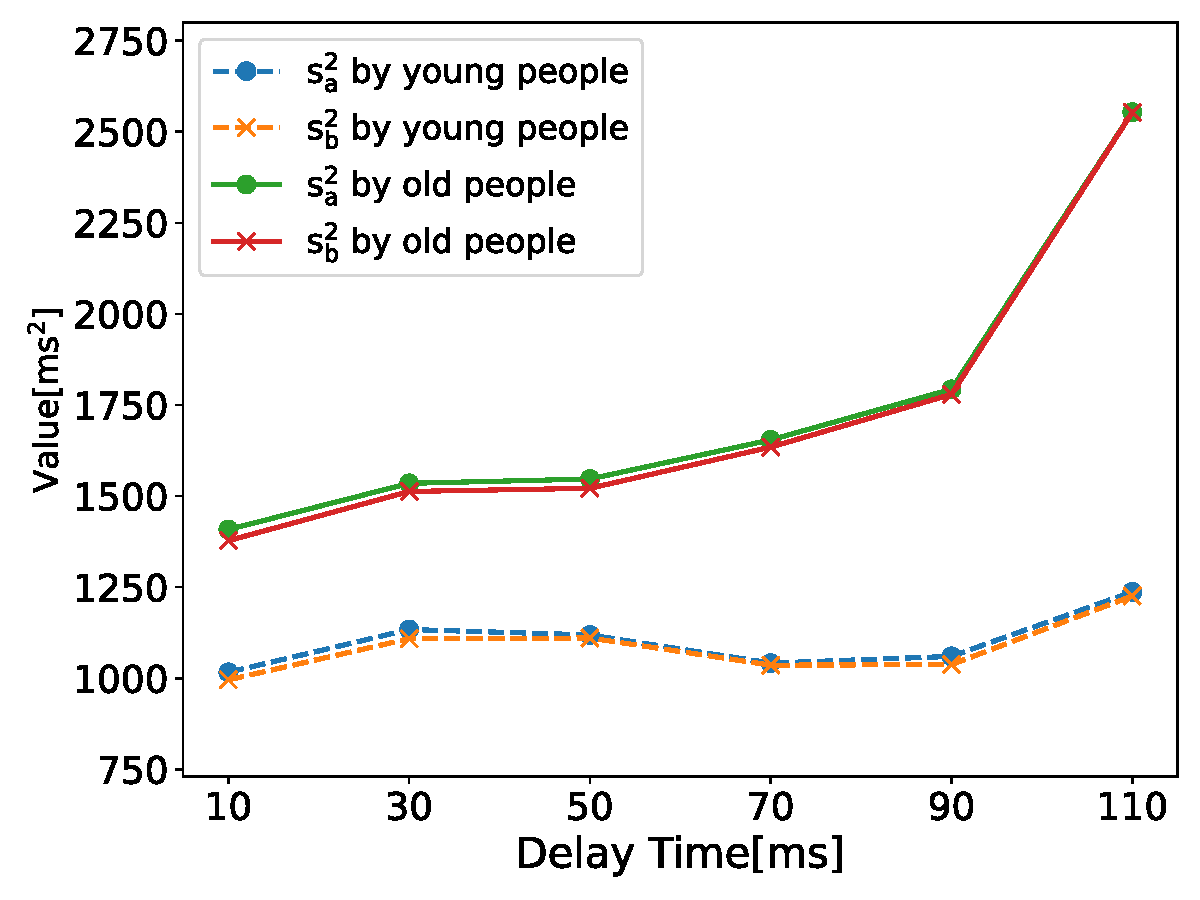
\includegraphics[scale=0.5]{figures/Honbann/Comparison_young_old/110_var_SaSb.pdf}
  \caption{実験Aにおける若年者と高齢者の分散の比較}
  \label{fig:Var_110ms_Sa_Sb}
\end{figure}
\begin{figure}[tbp]
  \centering
  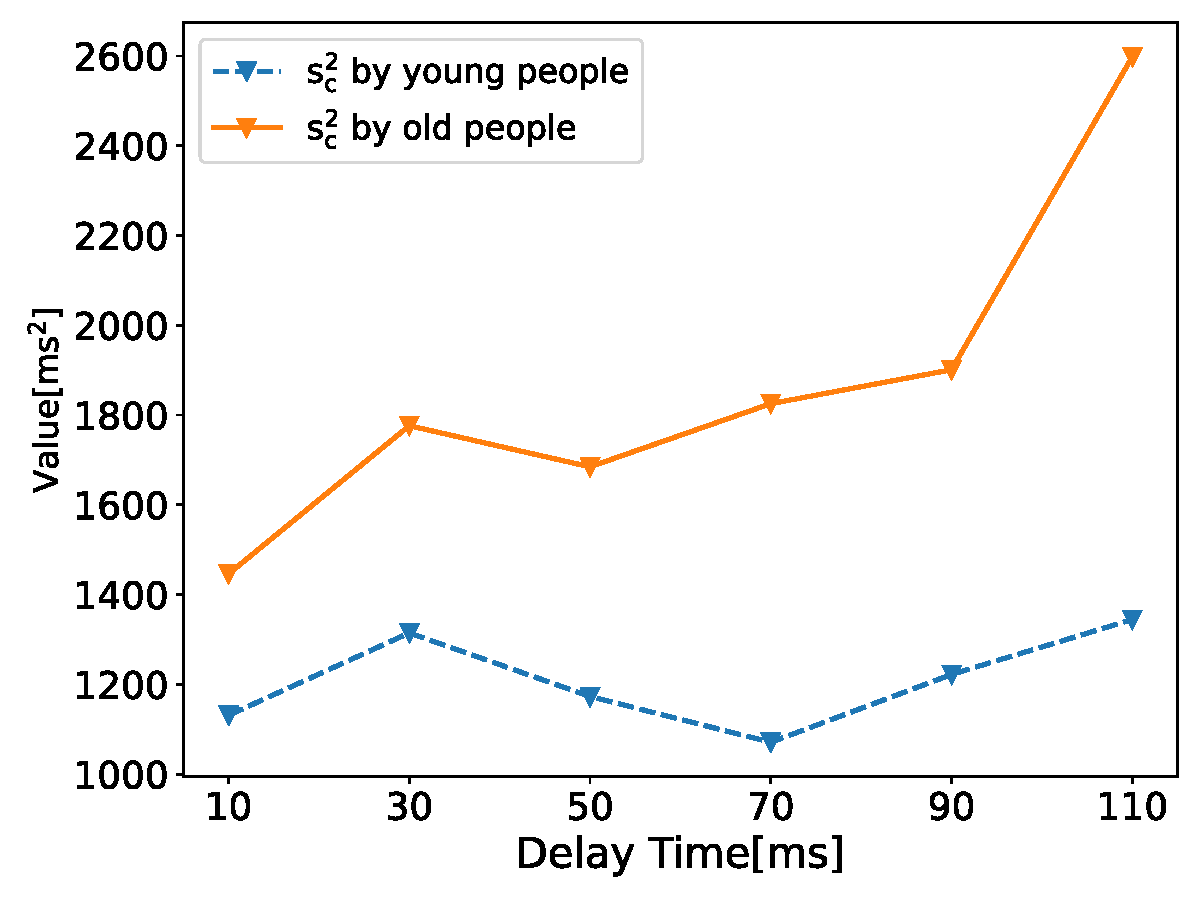
\includegraphics[scale=0.5]{figures/Honbann/Comparison_young_old/110_var_Sc.pdf}
  \caption{実験Aにおける若年者と高齢者の分散の比較}
  \label{fig:Var_110ms_Sc}
\end{figure}

\begin{figure}[tbp]
  \centering
  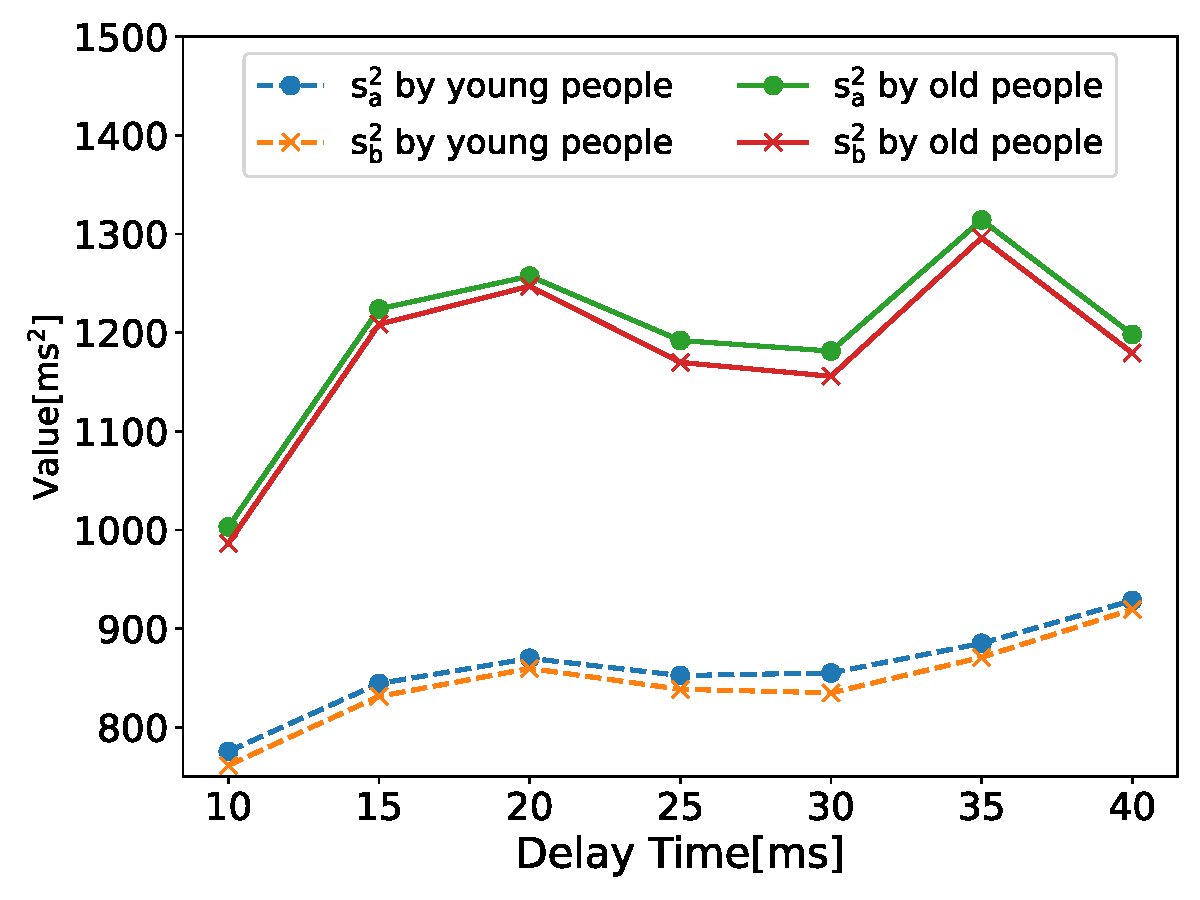
\includegraphics[scale=0.5]{figures/Honbann/Comparison_young_old/40_var_SaSb.pdf}
  \caption{実験Bにおける若年者と高齢者の分散の比較}
  \label{fig:Var_40ms_Sa_Sb}
\end{figure}

\begin{figure}[tbp]
  \centering
  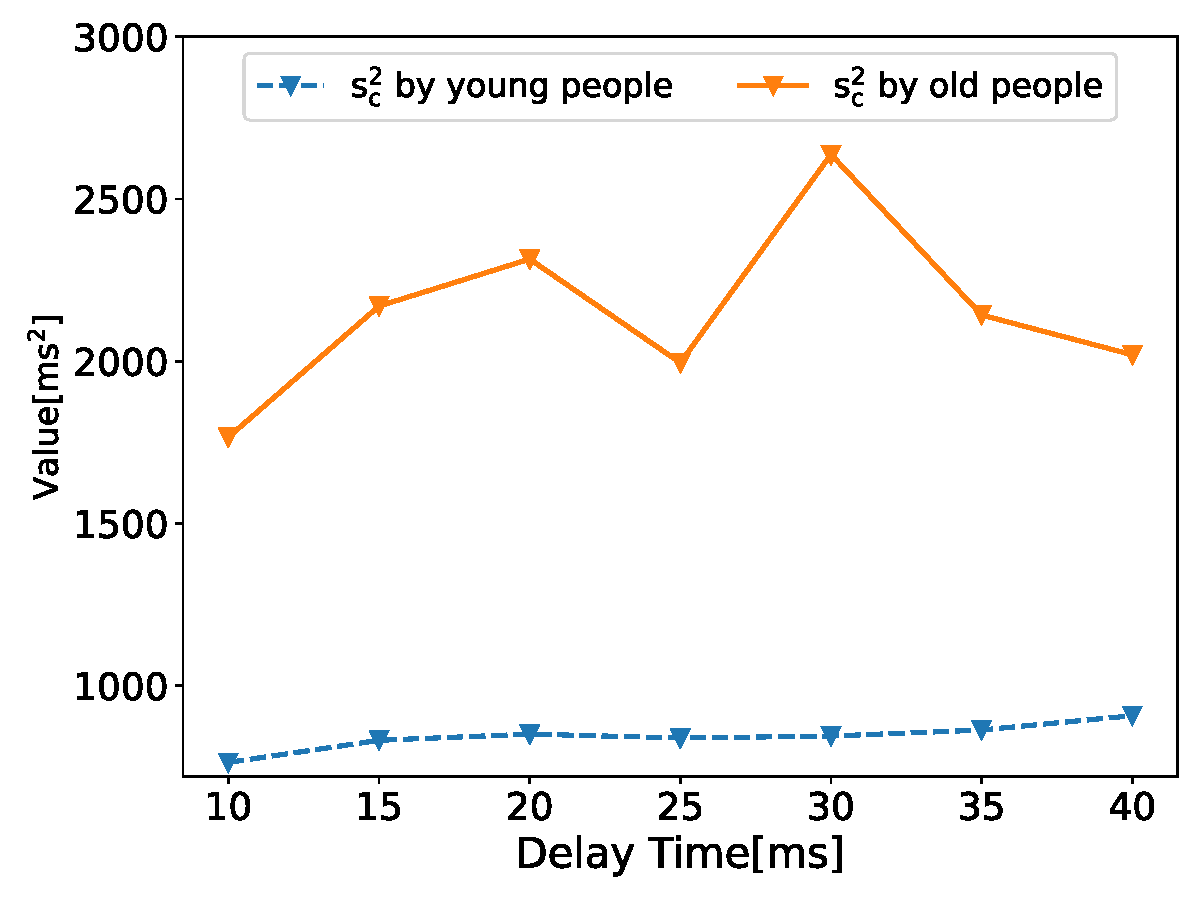
\includegraphics[scale=0.5]{figures/Honbann/Comparison_young_old/40_var_Sc.pdf}
  \caption{実験Bにおける若年者と高齢者の分散の比較}
  \label{fig:Var_40ms_Sc}
\end{figure}

%%%%%%%
% 正規化あり
%%%%%%%
\begin{figure}[tbp]
  \centering
  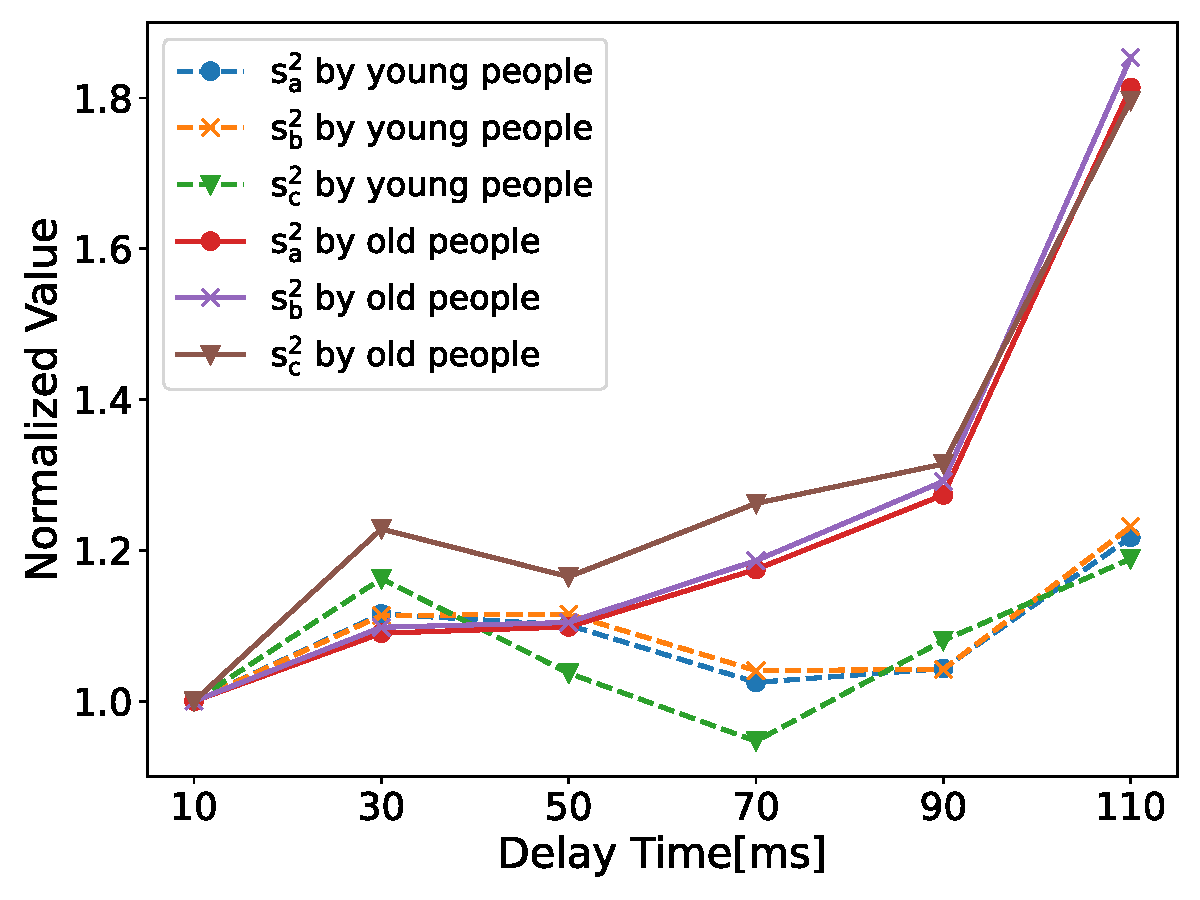
\includegraphics[scale=0.5]{figures/Honbann/Comparison_young_old/110_var_normalized.pdf}
  \caption{実験Aにおける若年者と高齢者の正規化後の評価値の比較}
  \label{fig:Normalized-Var_110ms_SaSbSc}
\end{figure}

\begin{figure}[tbp]
  \centering
  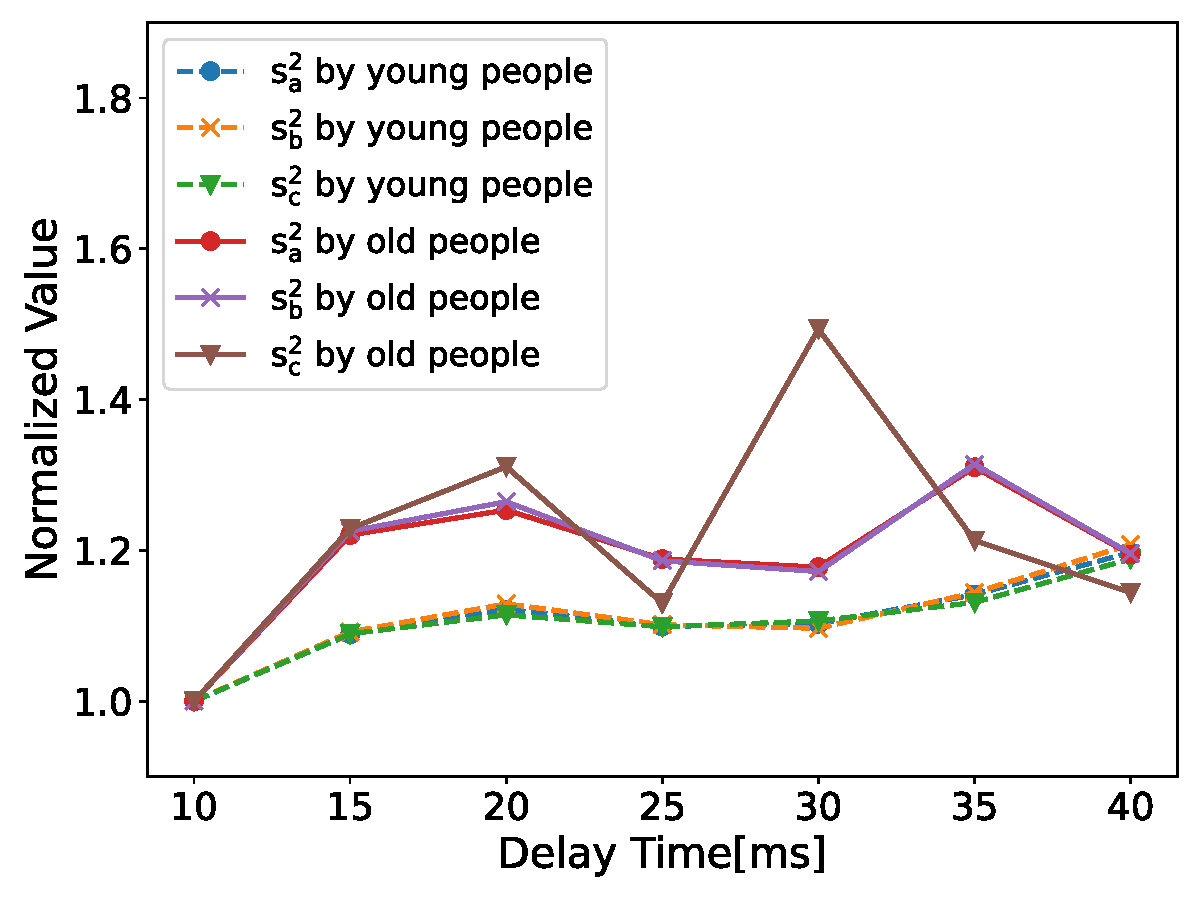
\includegraphics[scale=0.5]{figures/Honbann/Comparison_young_old/40_var_normalized.pdf}
  \caption{実験Bにおける若年者と高齢者の正規化後の評価値の比較}
  \label{fig:Normalized-Var_40ms_SaSbSc}
\end{figure}
 %%%%%%%%%%%%%%%%%%%%%%% ここまで

\begin{figure}[tbp]
  \centering
  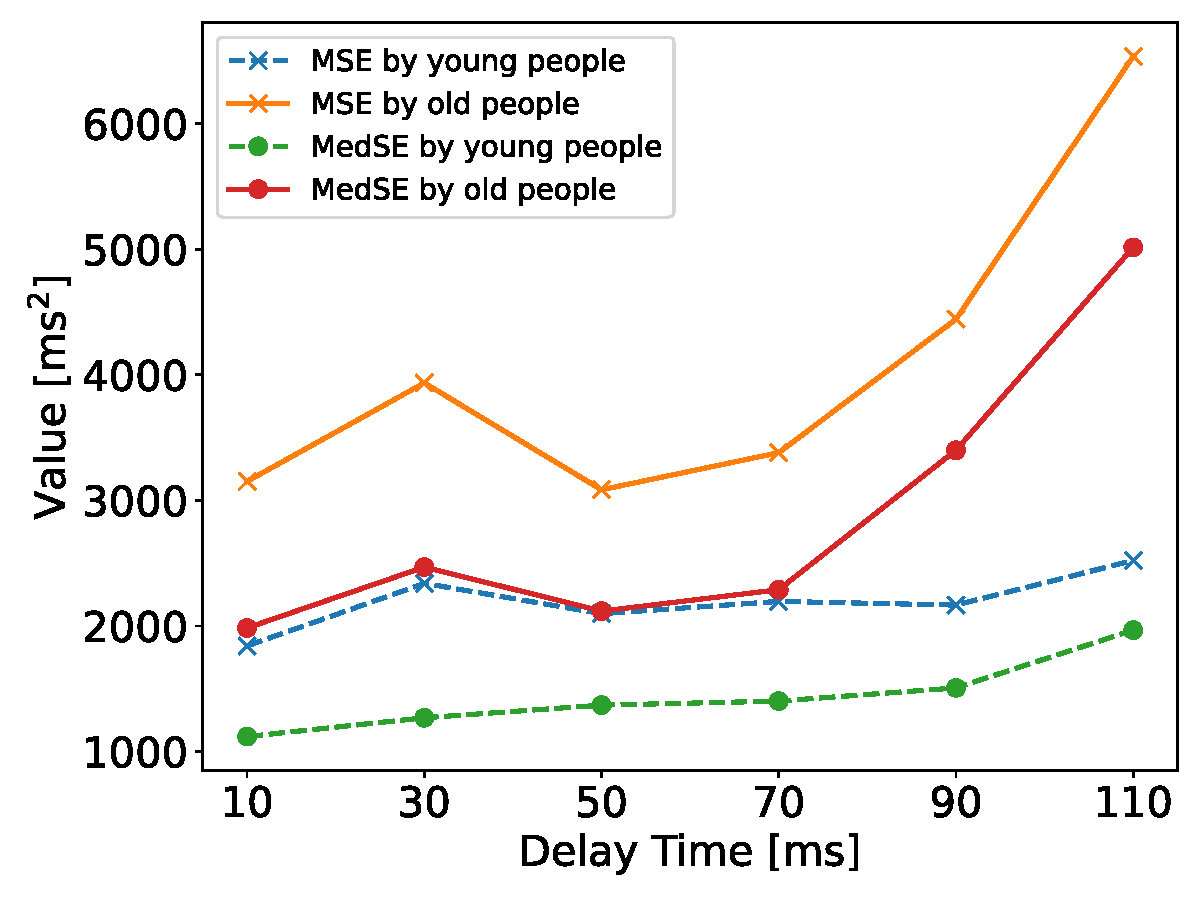
\includegraphics[scale=0.5]{figures/Honbann/Comparison_young_old/110_MSE-MedSE.pdf}
  \caption{実験Aにおける若年者と高齢者のMSEとMedSEの比較}
  \label{fig:110ms_MSE_MedSE}
\end{figure}
\begin{figure}[tbp]
  \centering
  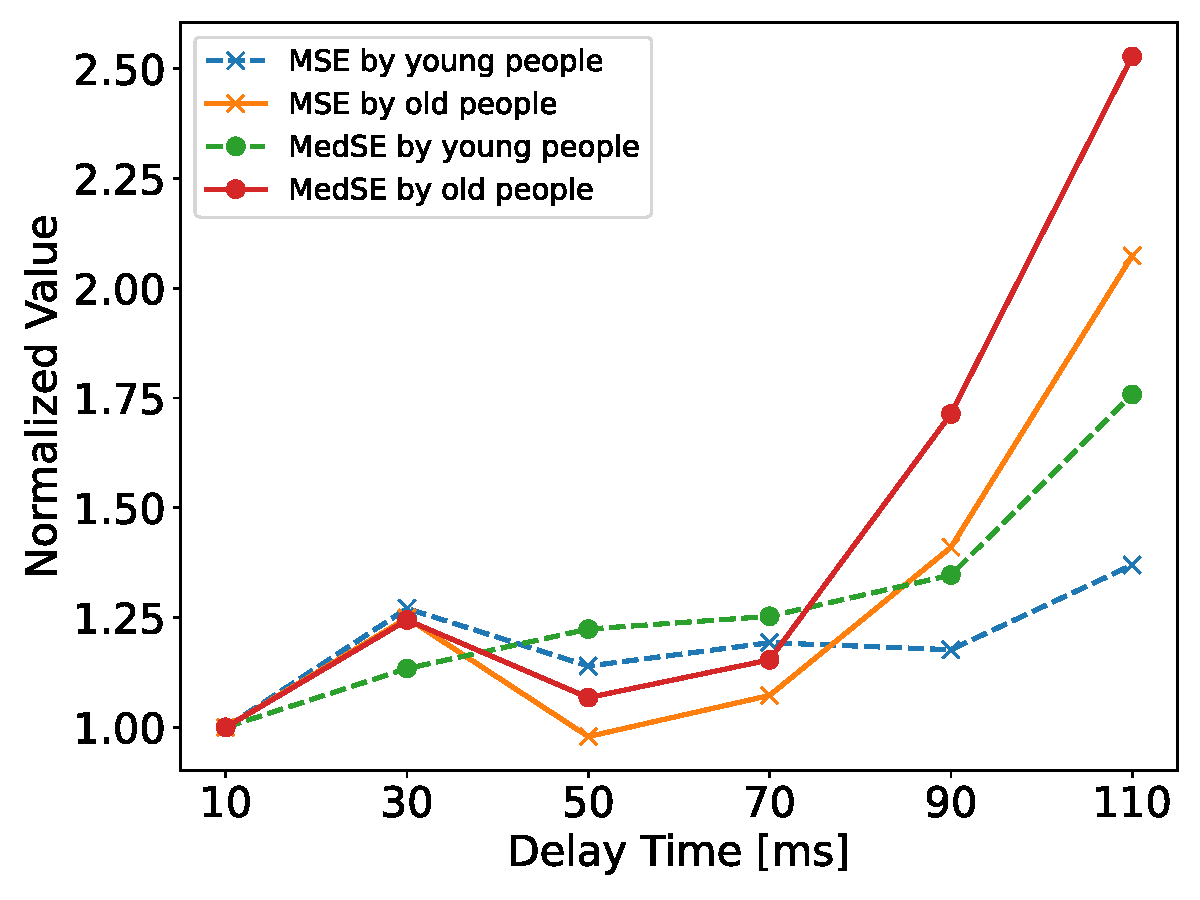
\includegraphics[scale=0.5]{figures/Honbann/Comparison_young_old/110_MSE-MedSE_normalized.pdf}
  \caption{実験Aにおける若年者と高齢者の正規化後のMSEとMedSEの比較}
  \label{fig:Normalized_110ms_MSE_MedSE}
\end{figure}
\begin{figure}[tbp]
  \centering
  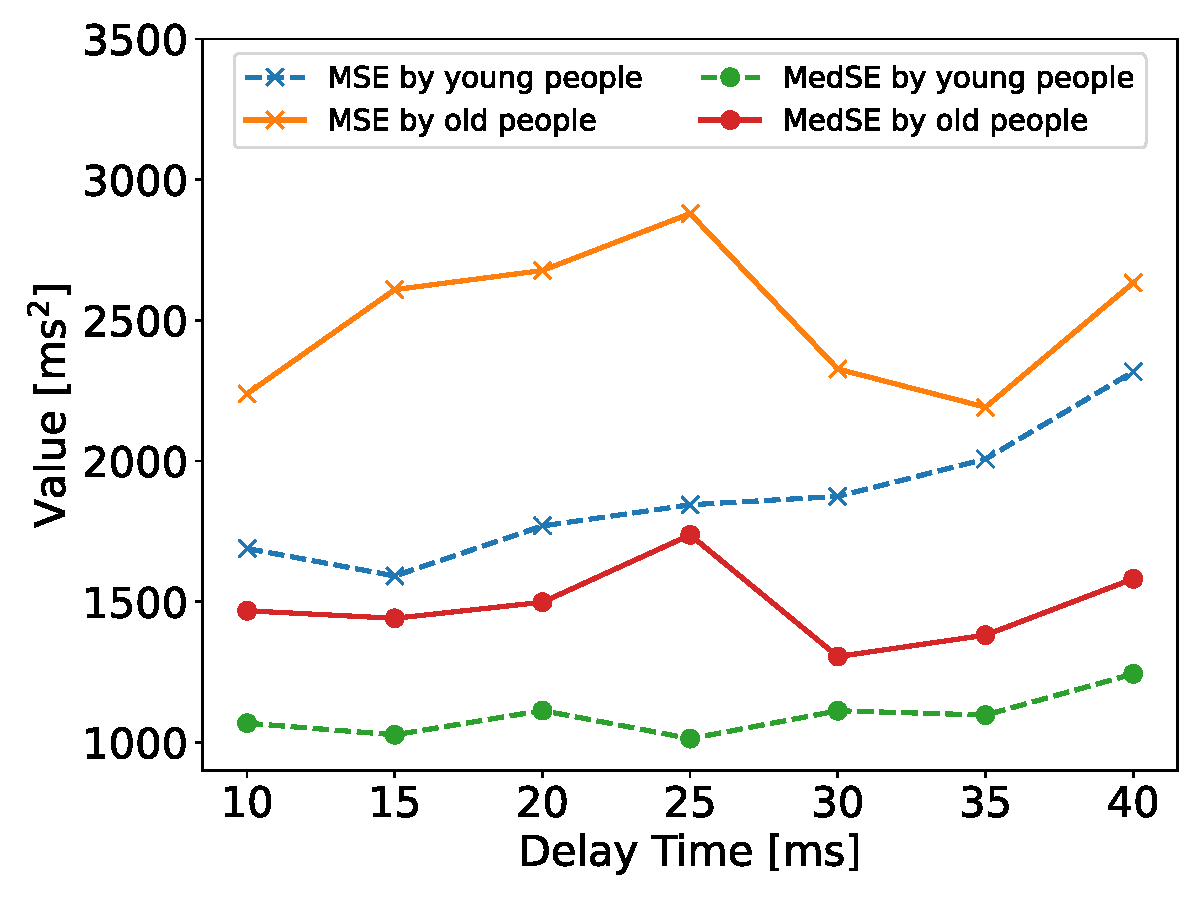
\includegraphics[scale=0.5]{figures/Honbann/Comparison_young_old/40_MSE-MedSE.pdf}
  \caption{実験Bにおける若年者と高齢者のMSEとMedSEの比較}
  \label{fig:40ms_MSE_MedSE}
\end{figure}

\begin{figure}[tbp]
  \centering
  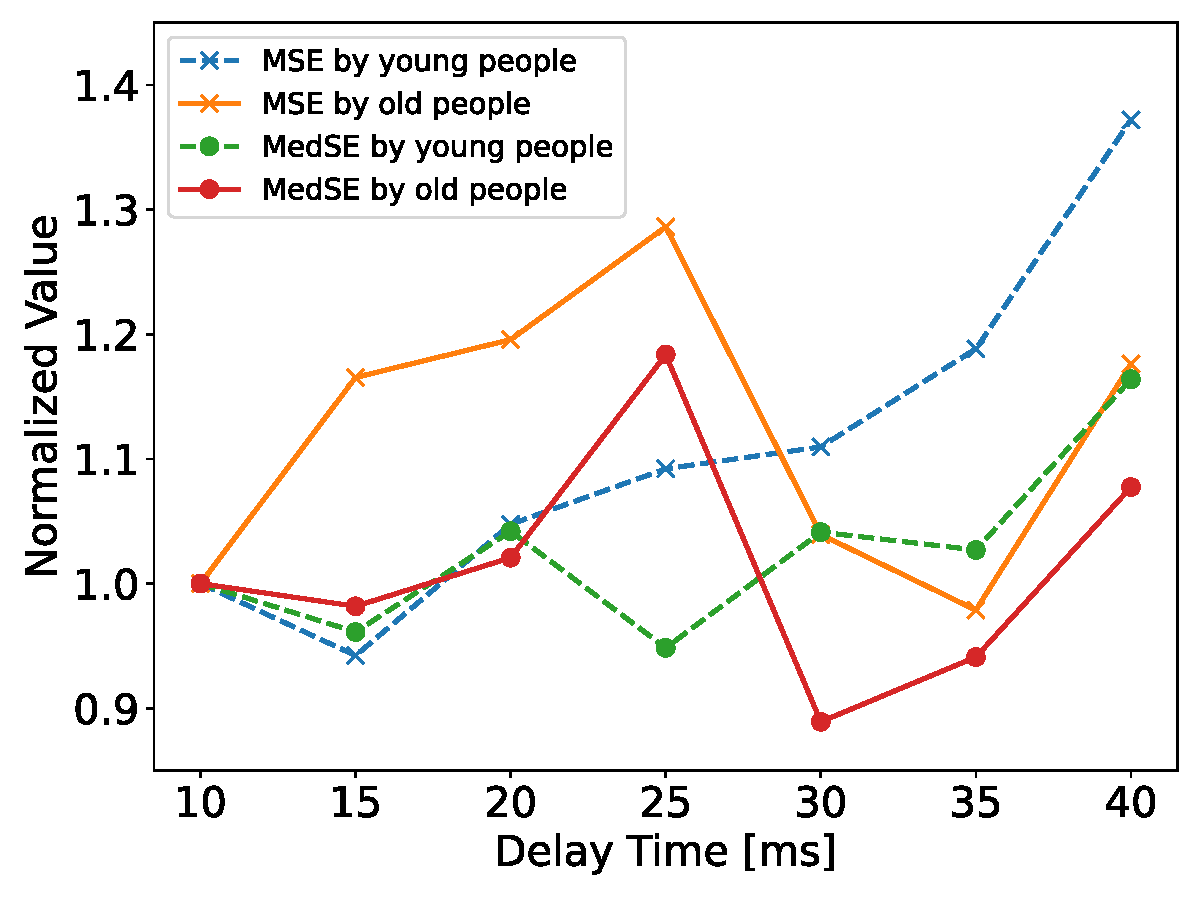
\includegraphics[scale=0.5]{figures/Honbann/Comparison_young_old/40_MSE-MedSE_normalized.pdf}
  \caption{実験Bにおける若年者と高齢者の正規化後のMSEとMedSEの比較}
  \label{fig:Normalized_40ms_MSE_MedSE}
\end{figure}
\chapter{結論}
\section{まとめ}
%%%%% 主観調査のためのアプリ開発 %%%%%
本研究では,将来的に実施予定の遅延聴覚フィードバックが発話に及ぼす影響の調査に向け,アプリケーションを開発した.
このアプリケーションにより,被験者がアプリケーション上に直接評価結果を入力し,その結果を外部ファイルに出力する機能を備えている.
この開発により,実験の効率化および評価結果の分析が容易になることが期待される.

%%%%%% 客観調査%%%%%%
また,聴覚フィードバックによる違和感を客観的に評価するために,先行研究で開発されたシステムを改良し,遅延聴覚フィードバックの
身体運動への影響をボタン押し課題を通じて調査した.
被験者は一定の時間間隔でボタンを押下し,ヘッドホンからの聴覚フィードバックの遅延がボタンの押下回数が4の倍数に達した際のみ発生する条件で課題を実施した.
この方法により,遅延聴覚フィードバックの影響によるボタンの押下間隔のばらつきを観察しやすくなるよう,客観的な評価指標および調査条件を定めた.
その結果,ボタン押し課題では,ボタンを押下する間隔を1分間に80回とし,
客観的な評価指標としてボタン押下間隔の平均及び中央値を真値とする分散,
およびボタンの押下回数が4の倍数に到達する直前の押下間隔と4の倍数に到達した直後の押下間隔の平均二乗誤差及び中央値二乗誤差を用いることが適切であると判断した.

そして,聴力の正常な若年者と高齢者を対象に,ボタン押し課題を用いて遅延聴覚フィードバックの身体運動への影響を調査した.
その結果,10msから40msの短い遅延時間では,若年者の評価値は遅延時間の増加に伴って,緩やかに増加する傾向が見られたが,
高齢者の評価値には一貫した関係が見出されなかった.
これは,若年者が遅延に敏感である一方で,高齢者が遅延時間に対して一定の許容度を持っていることを示している.
% 高齢者は若年者と比較して,聴覚フィードバックの遅延に対する許容度が高い可能性が示唆された.
遅延時間が10msから110msに及ぶ実験では,高齢者が遅延時間の増加に対して比較的鈍感であるものの,
一定の遅延時間を超えるとタスクの一貫性を保つことが困難になることが明らかになった.
これらの結果は,聴覚フィードバックの遅延に対する年齢別の感受性の違いを浮き彫りにし,高齢者向けの補聴器設計における重要な知見を提供するものであると考えられる.
さらに,高齢者が若年者に比べてすべての遅延時間で高い評価値を示したという結果は,高齢者と若年者間の潜在的な運動能力の差異がこれらの反応に影響している可能性を示唆している.
\section{今後の展望}
%%%%% 以下は,今後の展望の例 %%%%%
% ・3の倍数でもよくないか?\\
% ・聴力に異常がある人とない人では差があるのか?\\
% ・より細かい遅延時間で調査する必要があるのか?\\
% ・潜在的な身体能力の影響を軽減させるような課題を考える必要がある.
% 違和感を感じることと身体運動に影響があることは別のことである可能性がある.
% 客観調査と主観調査を同時に行うことで,遅延聴覚フィードバックが身体運動に与える影響をより詳細に調査することができると考えられる.
今後は,高齢者と若年者の運動能力の差異を調整し,遅延聴覚フィードバックの影響をより公平に評価するために,被験者の運動能力を考慮した課題を検討する必要がある.
運動能力の基本的な側面を評価するためのタスクを導入し,参加者の反応速度,精度,運動の一貫性を測定することで,運動能力の基準値を
設定し,遅延時間に対する反応の差異を適切に解釈することが可能になる.
また,課題の難易度や認知負荷を調整することで,運動能力以外の要因が遅延聴覚フィードバックの影響を受けるかどうかを評価することで,運動能力以外の能力が
影響を与える可能性を探ることができる.

%参考文献
\begin{thebibliography}{99}
	\bibitem{cf:a}細井裕司,``補聴器この20年間の進歩'' 日本耳鼻咽喉科科学会会報, 114巻,12号,pp.905-911,Jan.2015.
	\bibitem{cf:b}河原英紀,``聴覚フィードバックの発話への影響:ヒトは自分の話声を聞いているのか?'' 日本音響学会誌, 59巻, 11号, pp.670-675, Nov.2003
  \bibitem{cf:c}香山実結花,山下一樹,丹治寛樹,村上隆啓,``若年者と高齢者の聴覚フィードバックにおける遅延時間の許容量の統計的分析による比較'' 2022年度電子情報通信学会東京支部学生会研究発表会, pp.113,Mar.2023
  \bibitem{cf:d}重松颯人,丹治寛樹,村上隆啓,松本直樹,``遅延聴覚フィードバックが身体運動に与える影響の客観的な評価方法の検討'' 日本音響学会聴覚研究会資料, pp.499-504, Nov.2019
  \bibitem{cf:e}著者名,``題目'' 出典論文誌名, Vol. XX, No. YY, pp.ZZ1--ZZ2, Sep,2011
  \bibitem{cf:f}著者名,``題目'' 出典論文誌名, Vol. XX, No. YY, pp.ZZ1--ZZ2, Sep,2011


\end{thebibliography}
\begin{thepublished}{99}
	\bibitem{cf:c}山下一樹,安田和生,丹治寛樹,村上隆啓,``若年者と高齢者の遅延聴覚フィードバックの身体運動への影響の比較'' 2023年度電子情報通信学会東京支部学生会, Vol. XX, No. YY, pp.ZZ1--ZZ2, Sep,2011
	
\end{thepublished}
\newpage

\begin{acknowledgement}
本研究を進めるにあたり,多大なるご指導,
ご助言を頂きました明治大学理工学部電気電子生命学科所属の村上隆啓専任講師に心から感謝いたします.
また,日頃の研究活動及び本論文に多大なご助言を頂きました,明治大学理工学部電気電子生命学科所属の丹治寛樹助教に心から感謝いたします.
遅延時間の許容調査における被験者募集にご協力いただいた情報科学科の井口幸洋教授及び井口道子様,明大サポートの山本様,福島様にも感謝の意を表します.
また,本研究にご協力いただいた多くの被験者の方々に厚く御礼申し上げます.
共同研究者として多くのご協力を頂いた知能信号処理研究室所属の安田和生氏と研究に関しまして多数のご助言をくださいました知能信号処理研究室の同期と後輩の皆様に心から感謝いたします.
\makesignature
\end{acknowledgement}


\appendix
\chapter{遅延聴覚フィードバックが身体運動に与える影響の調査の資料}
% 付録を掲載する場合,\verb|\chapter|コマンドの前に\verb|\appendix|コマンドを入れてください.
遅延聴覚フィードバックが身体運動に与える影響の調査を行うときに用いた,
研究参加同意書(明治大学生用・明治大学生以外の60歳未満の方用・明治大学生以外の60歳以上の方用),実験概要説明ボード(60歳の未満の方用・60歳以上の方用),聴力検査手順説明ボード,実験手順説明ボード,音量調整ボードを掲載する.
\begin{figure}[ht]
	\centering
	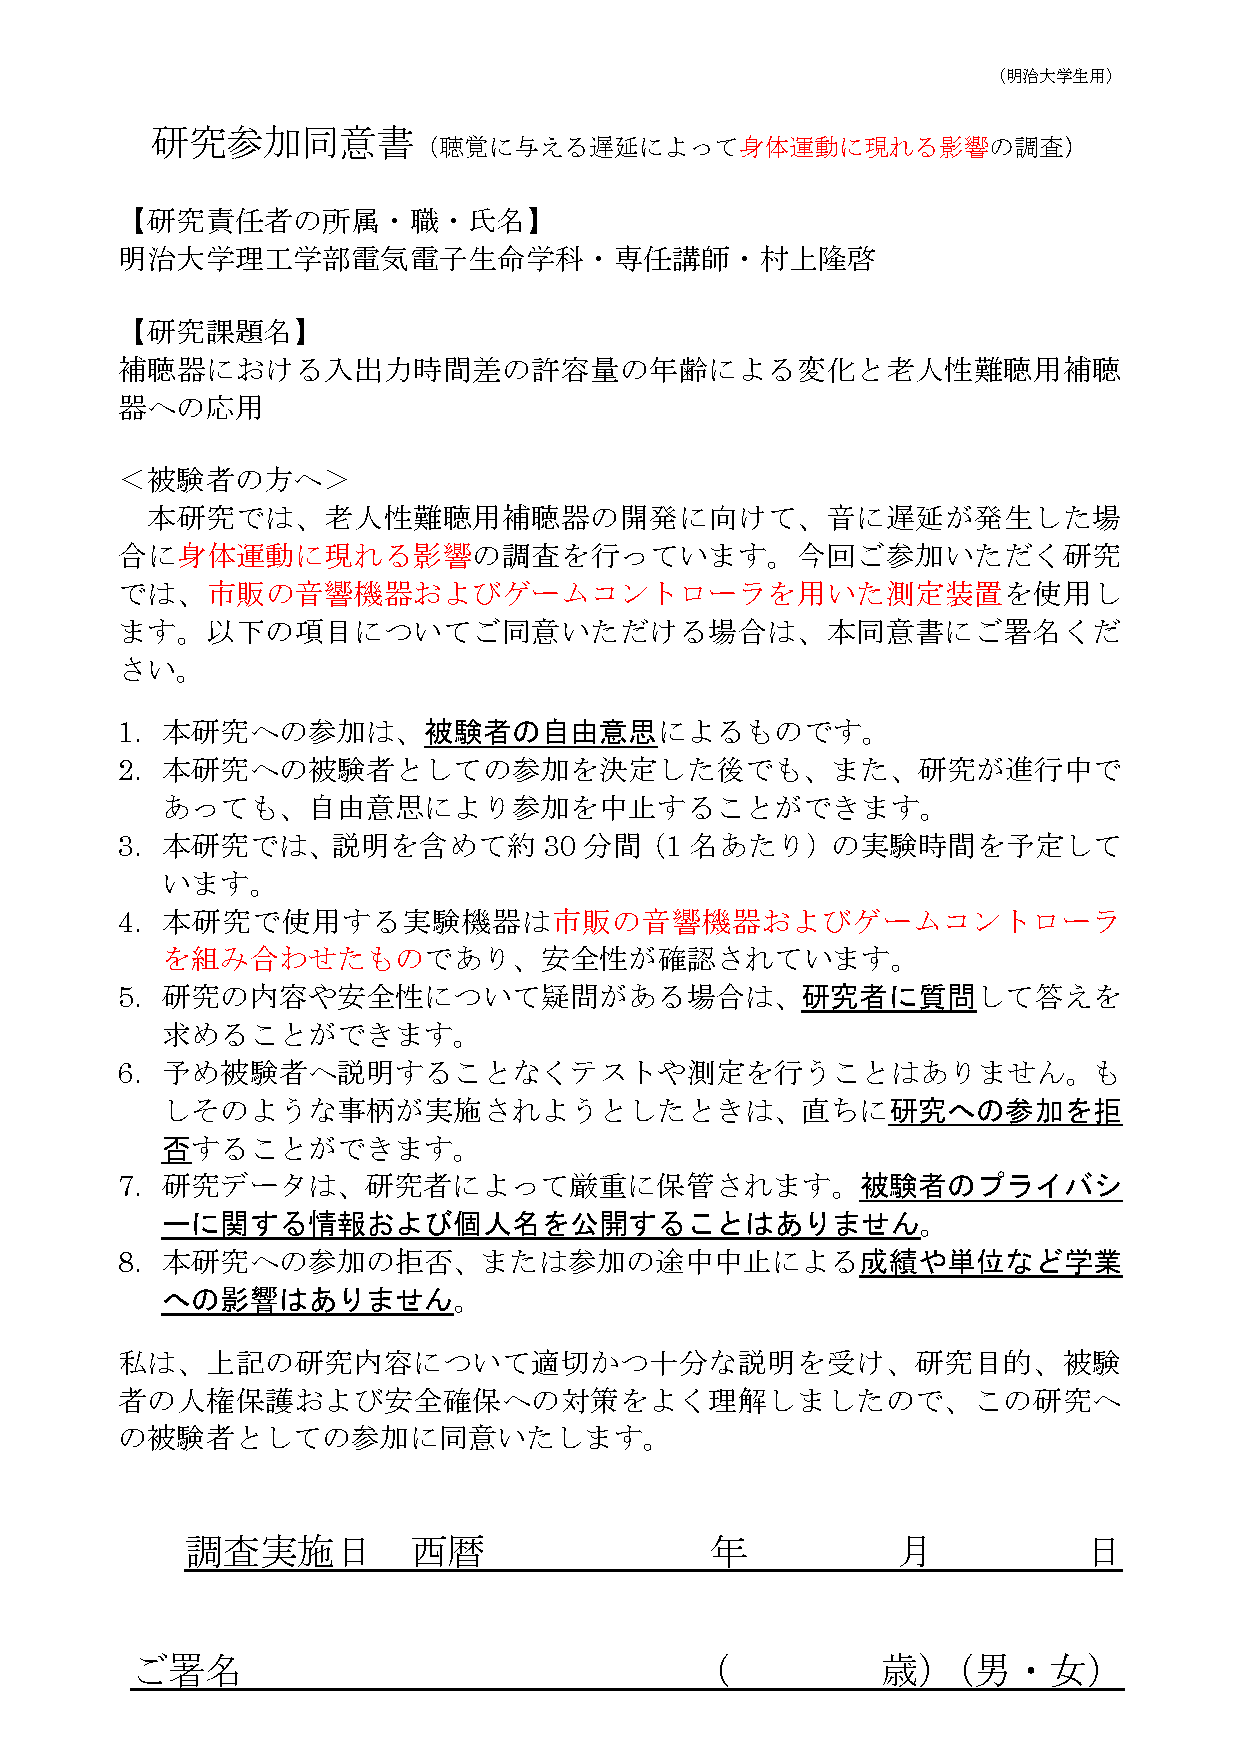
\includegraphics[width=\textwidth]{furoku_A/douisyo_meiji.pdf} % 画像の幅をテキストの幅に合わせる
	\caption{研究参加同意書(明治大学生用)}
\end{figure}
\begin{figure}[ht]
  \centering
  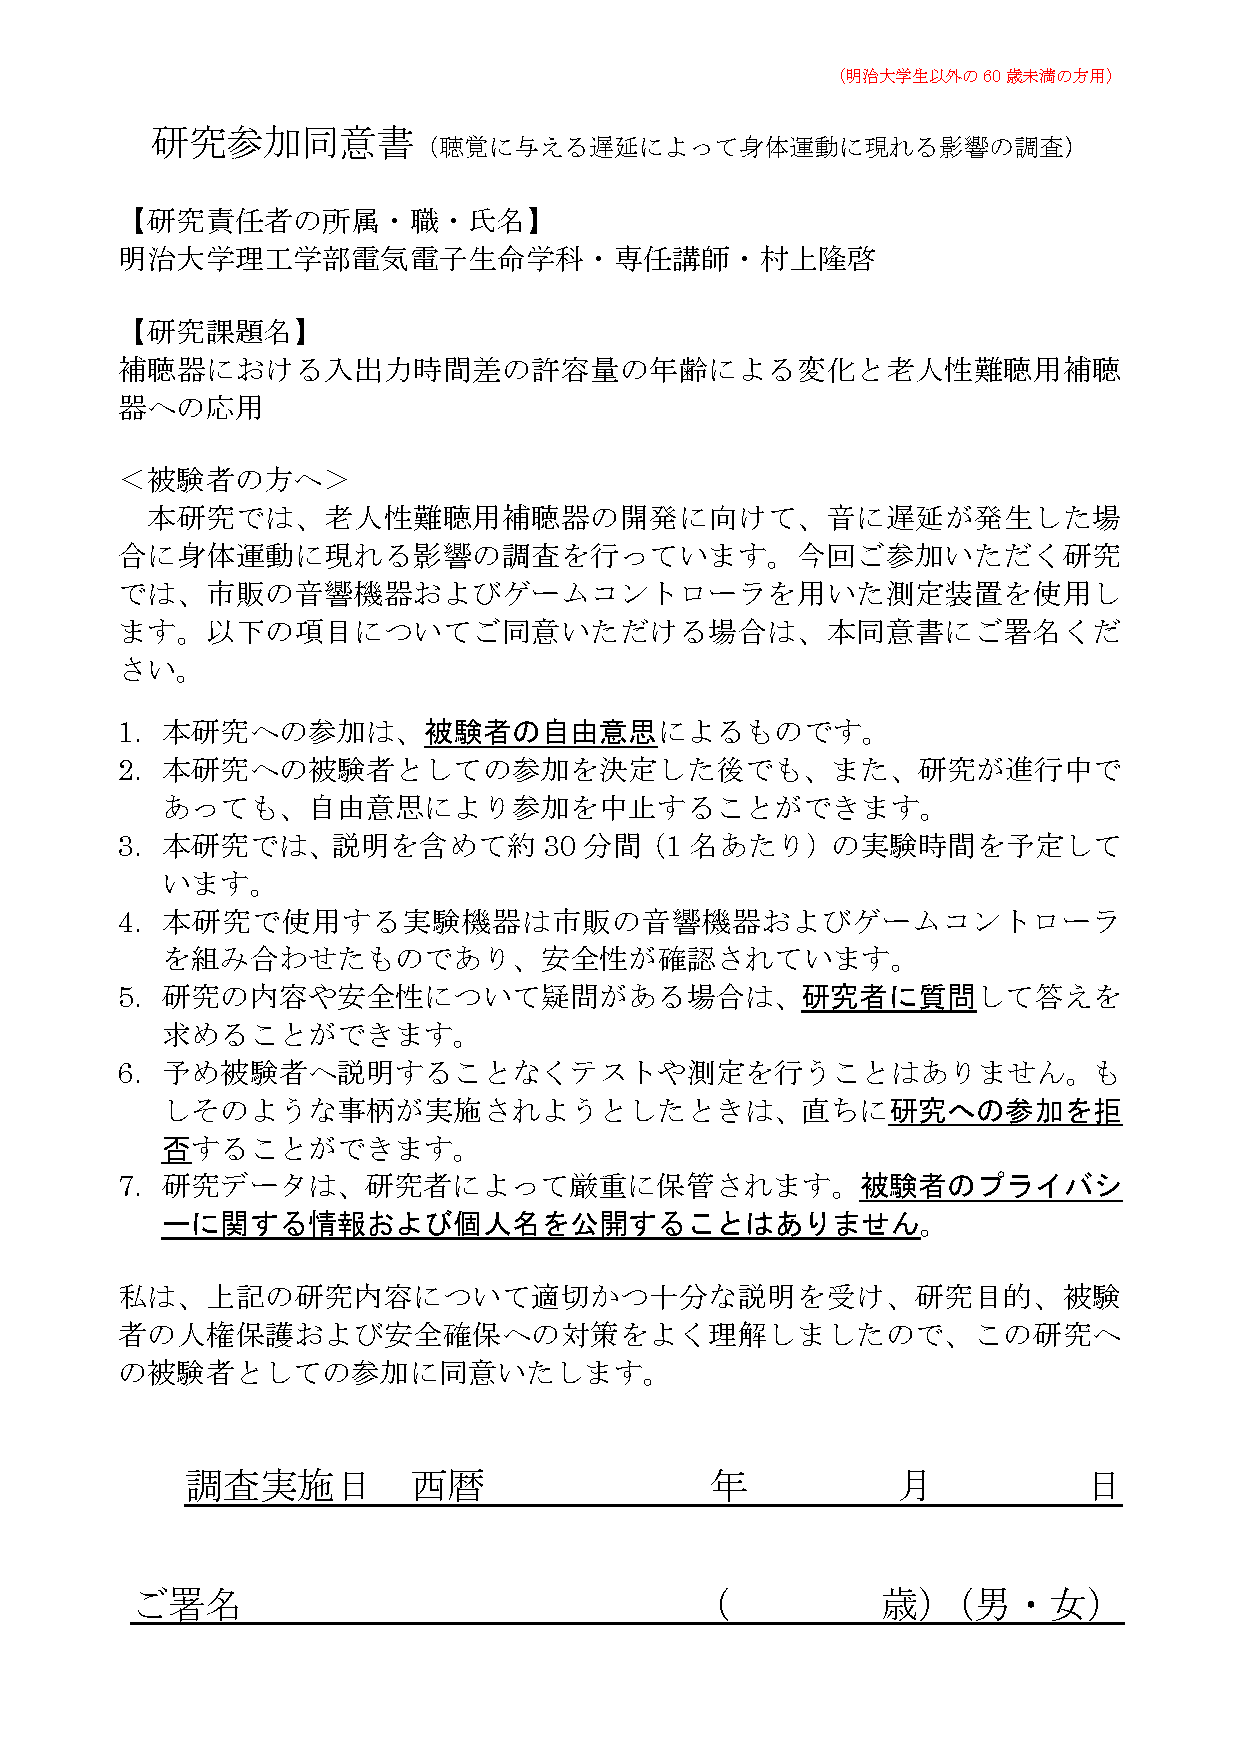
\includegraphics[scale=0.6]{furoku_A/Douisyo_Not60NotMeiji.pdf}
  \caption{研究参加同意書(明治大学生以外の60歳未満の方用)}
\end{figure}
\begin{figure}[ht]
  \centering
  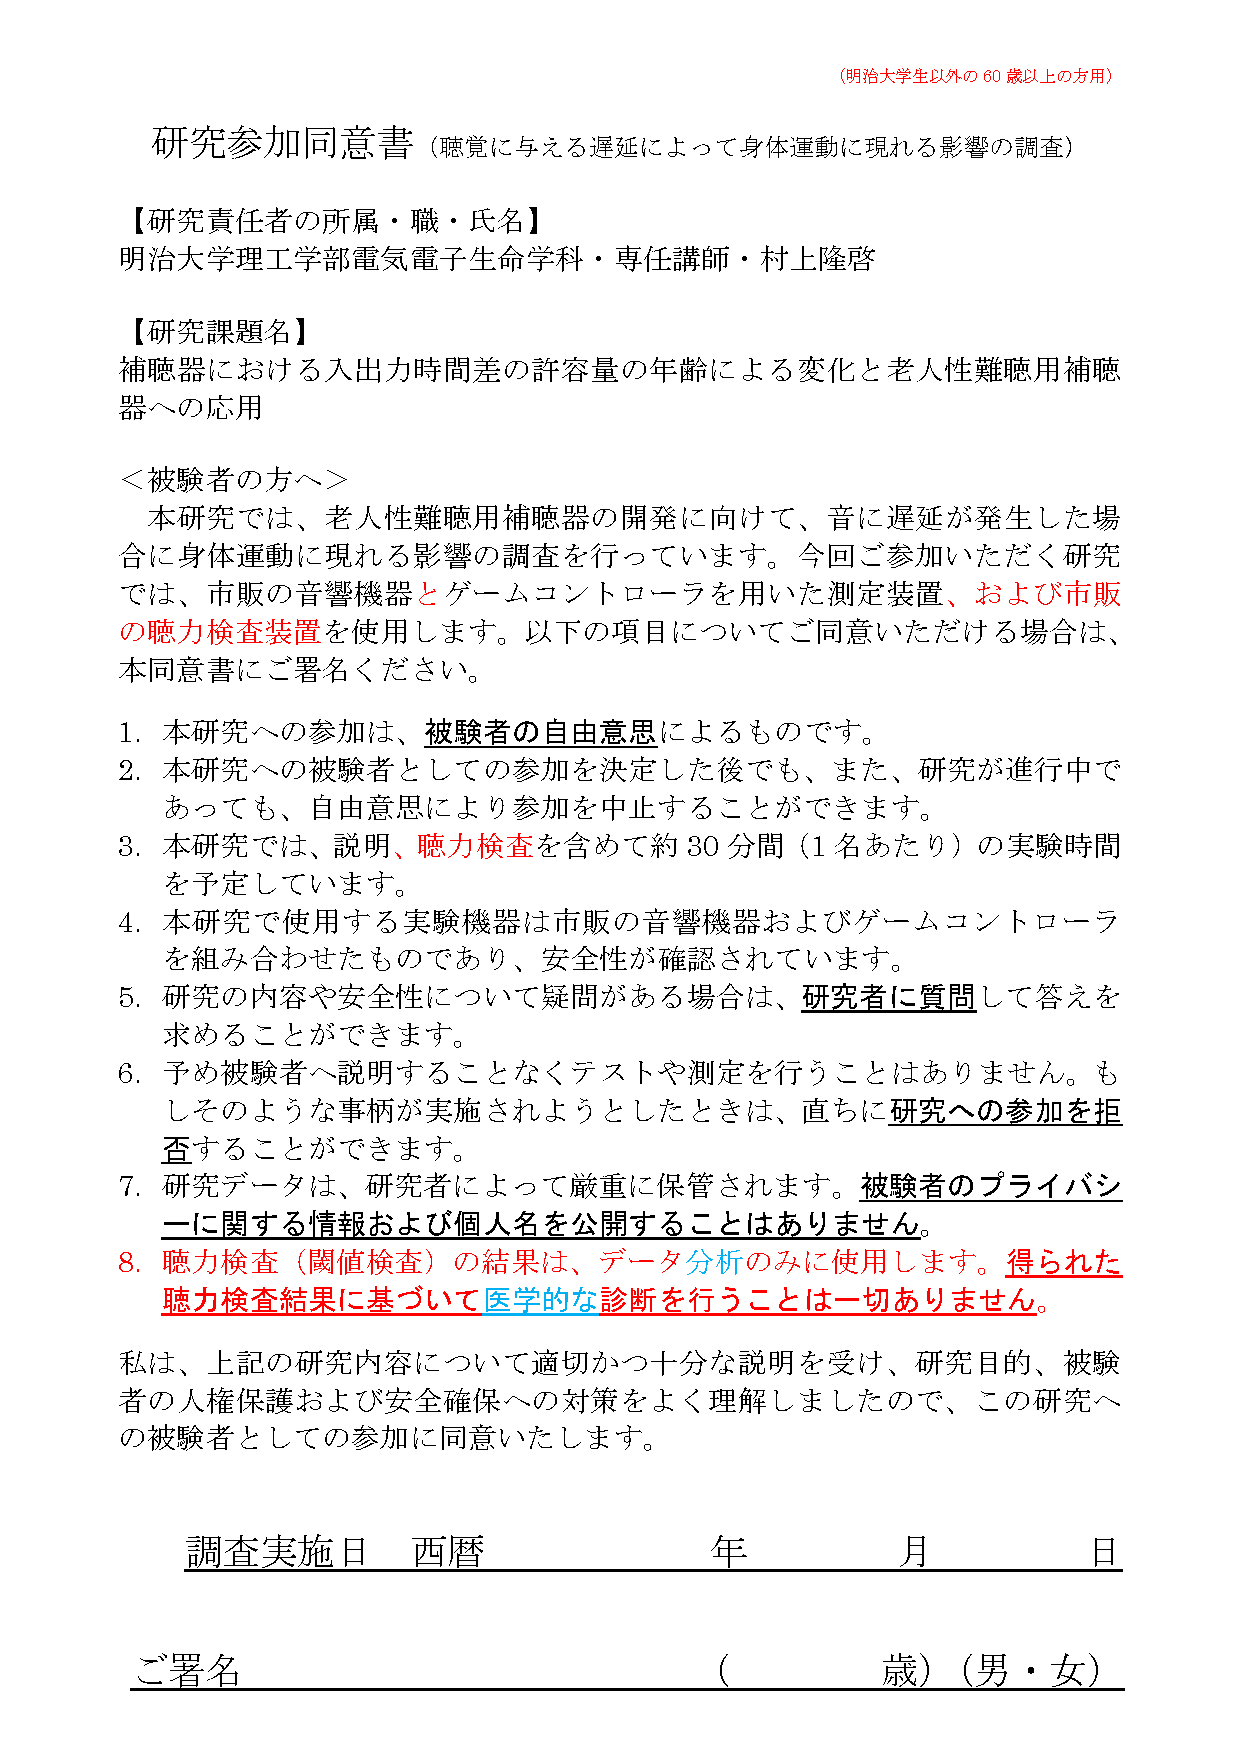
\includegraphics[scale=0.6]{furoku_A/Douisyo_60NotMeiji.pdf}
  \caption{研究参加同意書(明治大学生以外の60歳以上の方用)}
\end{figure}
\begin{figure}[ht]
  \centering
  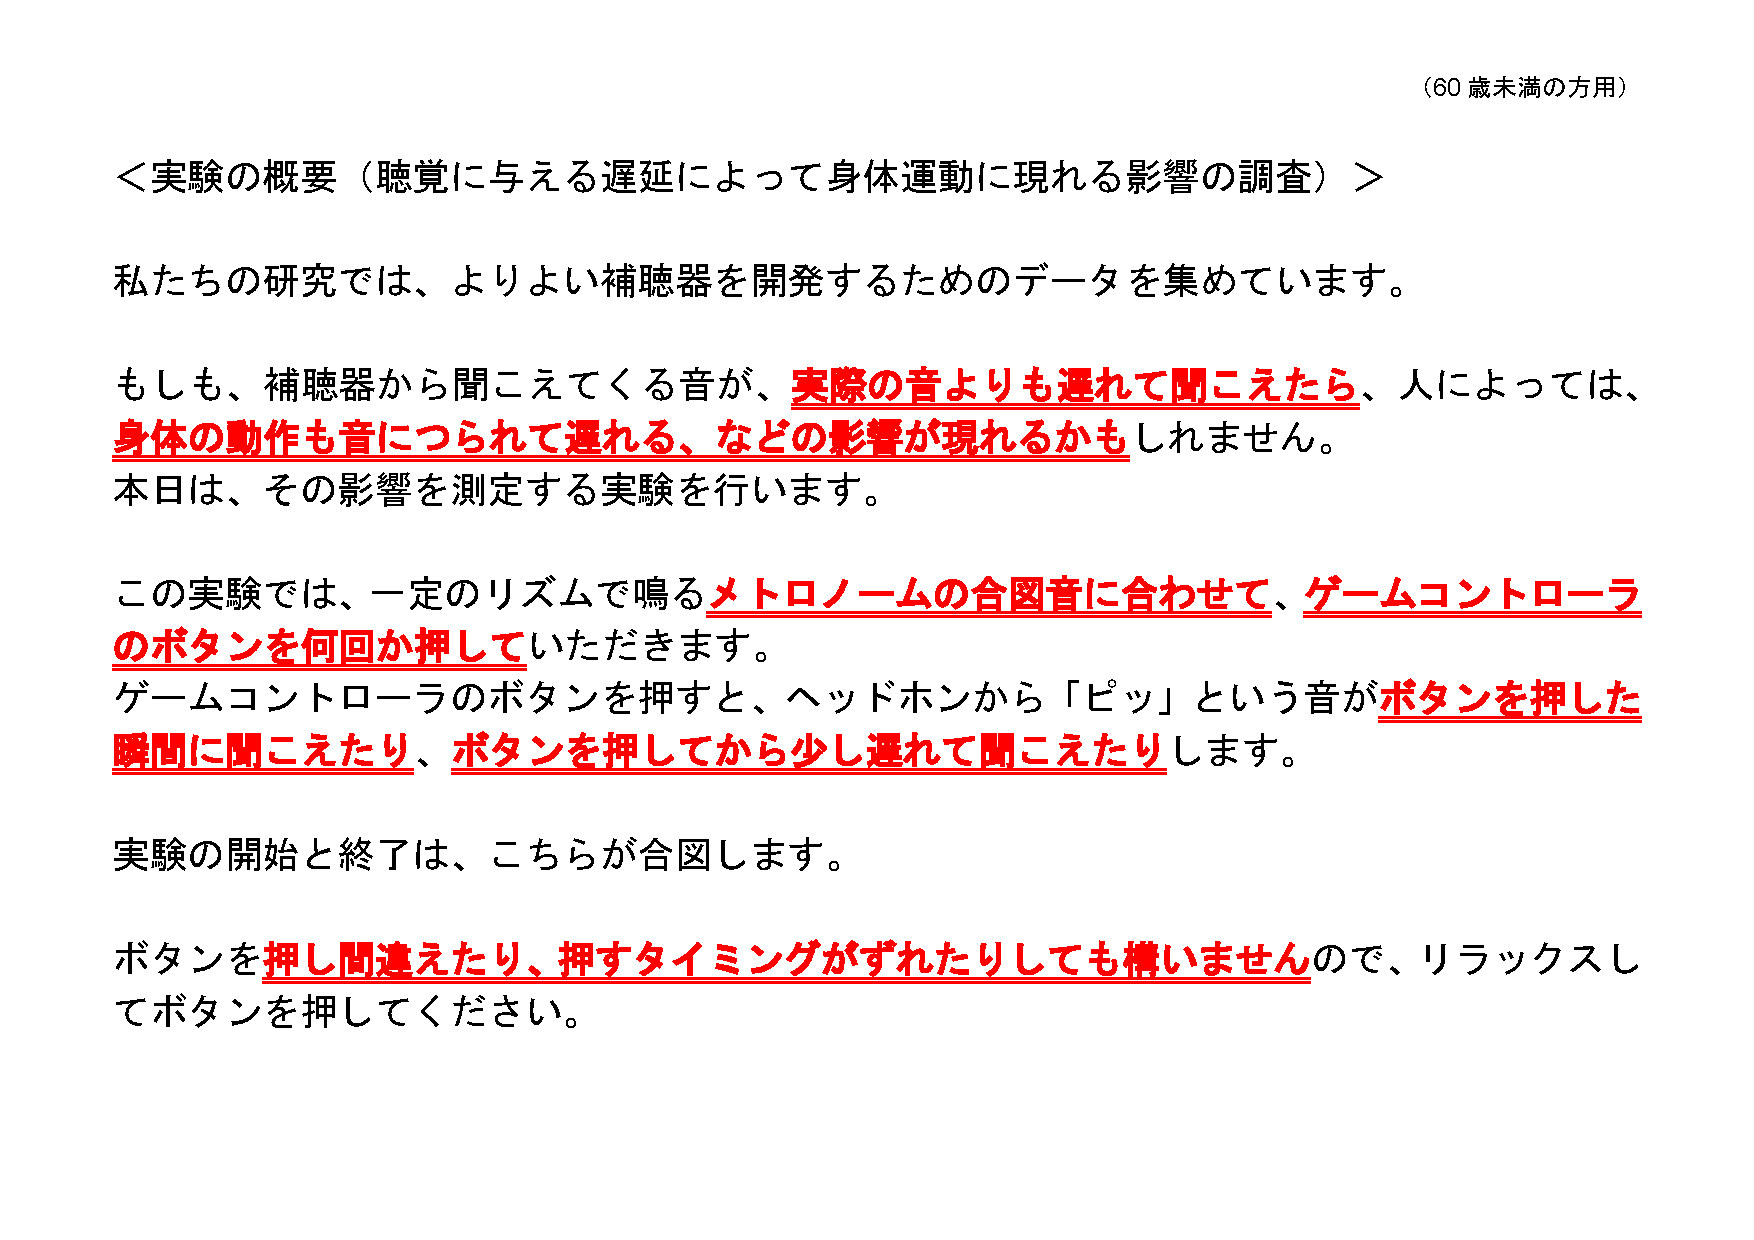
\includegraphics[scale=0.4]{furoku_A/Less60_gaiyou.pdf}
  \caption{実験概要説明ボード(60歳未満の方用)}
\end{figure}
\begin{figure}[ht]
  \centering
  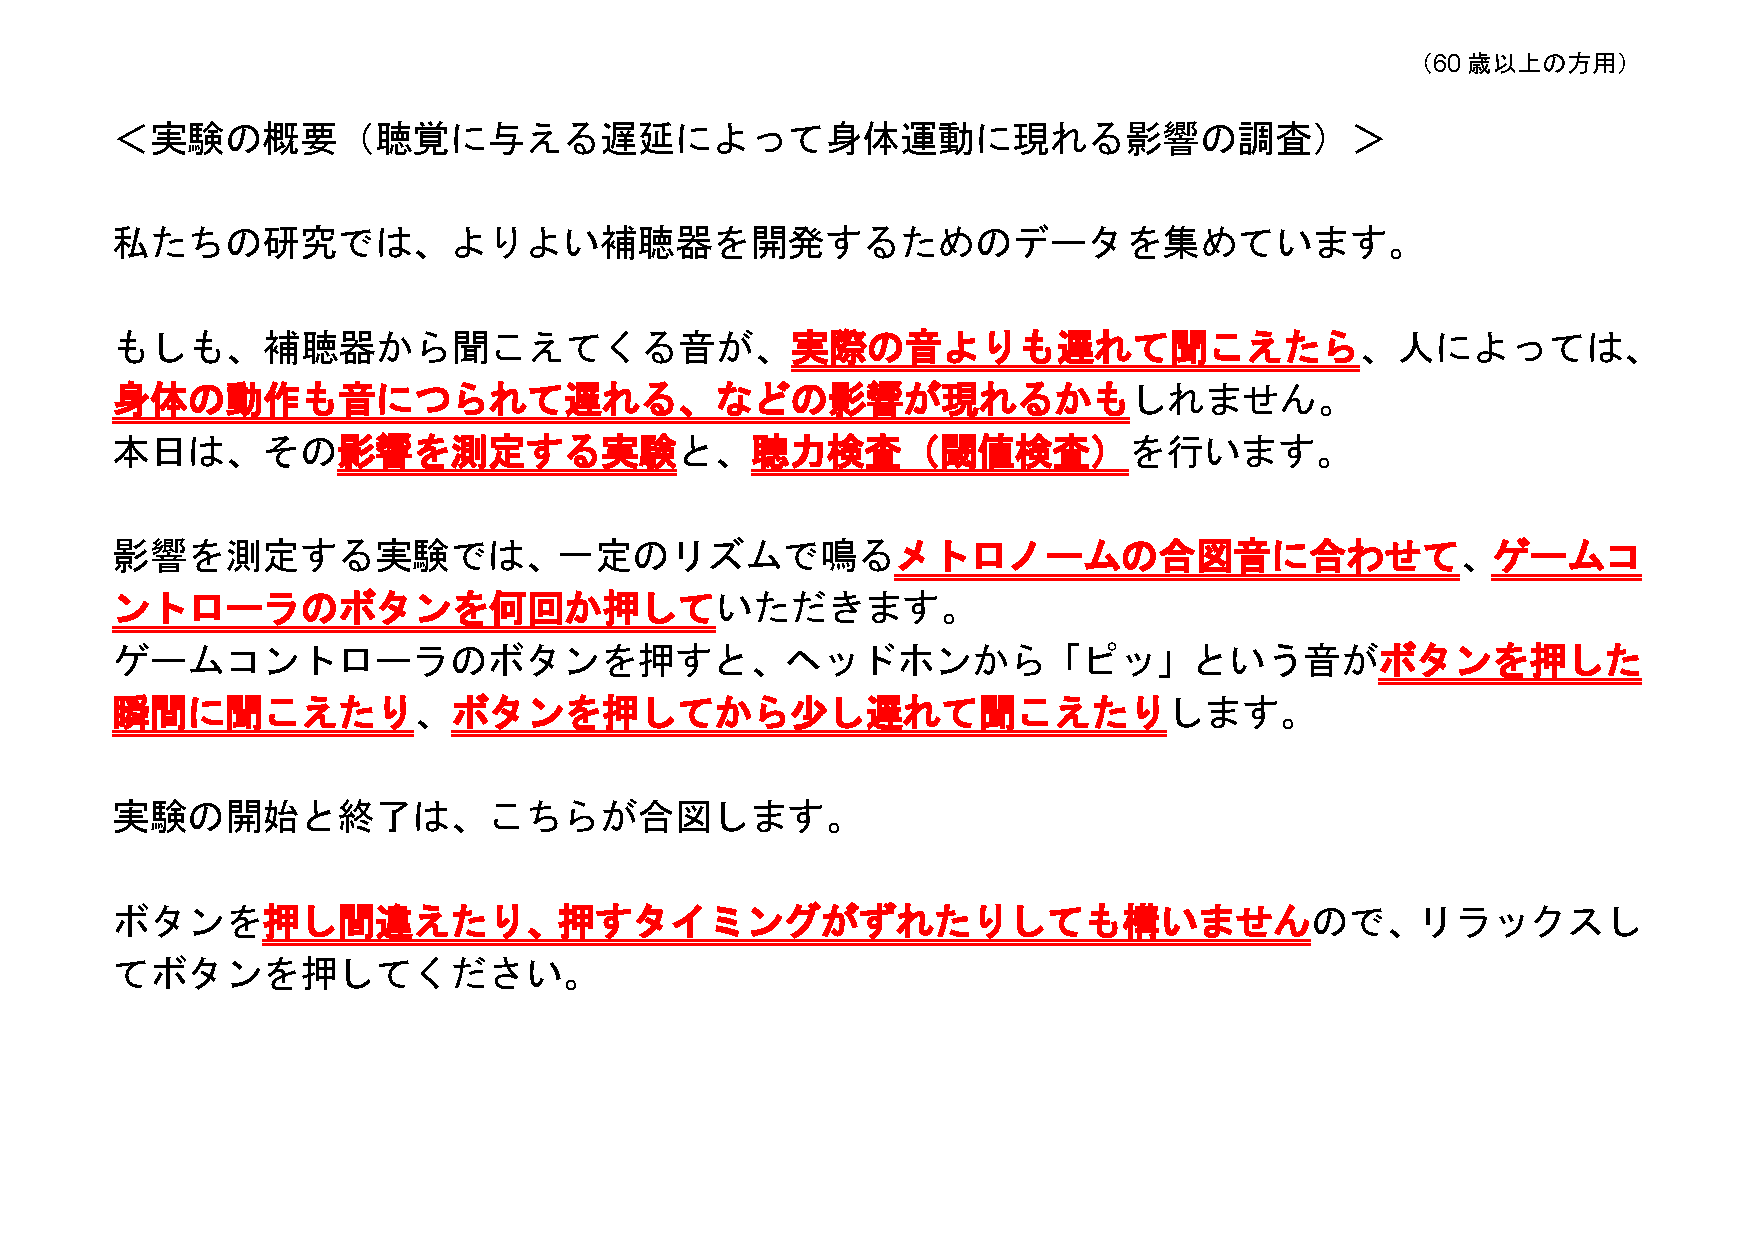
\includegraphics[scale=0.4]{furoku_A/MoreThan60_Gaiyou.pdf}
  \caption{実験概要説明ボード(60歳以上の方用)}
\end{figure}
\begin{figure}[ht]
  \centering
  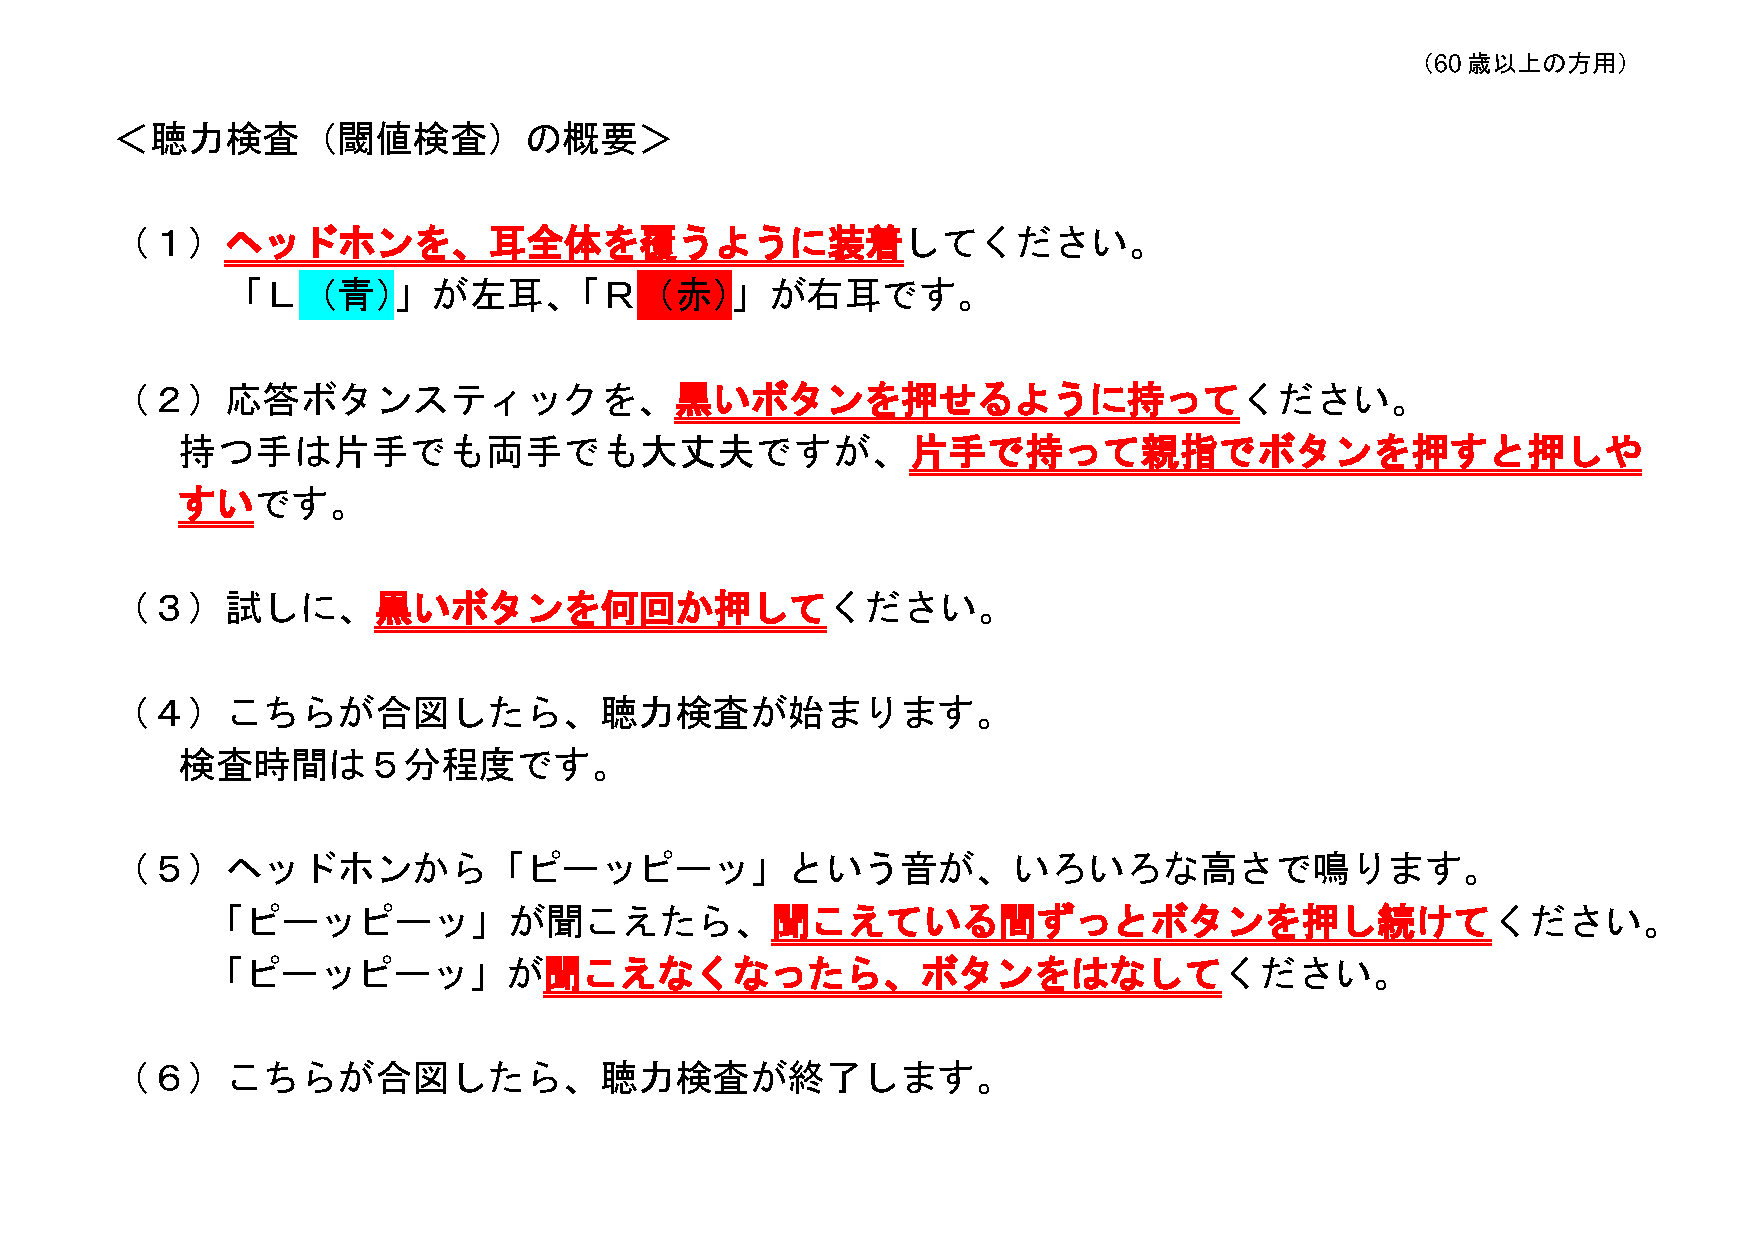
\includegraphics[scale=0.4]{furoku_A/MoreThan60_tyouryoku.pdf}
  \caption{聴力検査手順説明ボード}
\end{figure}
\begin{figure}[ht]
  \centering
  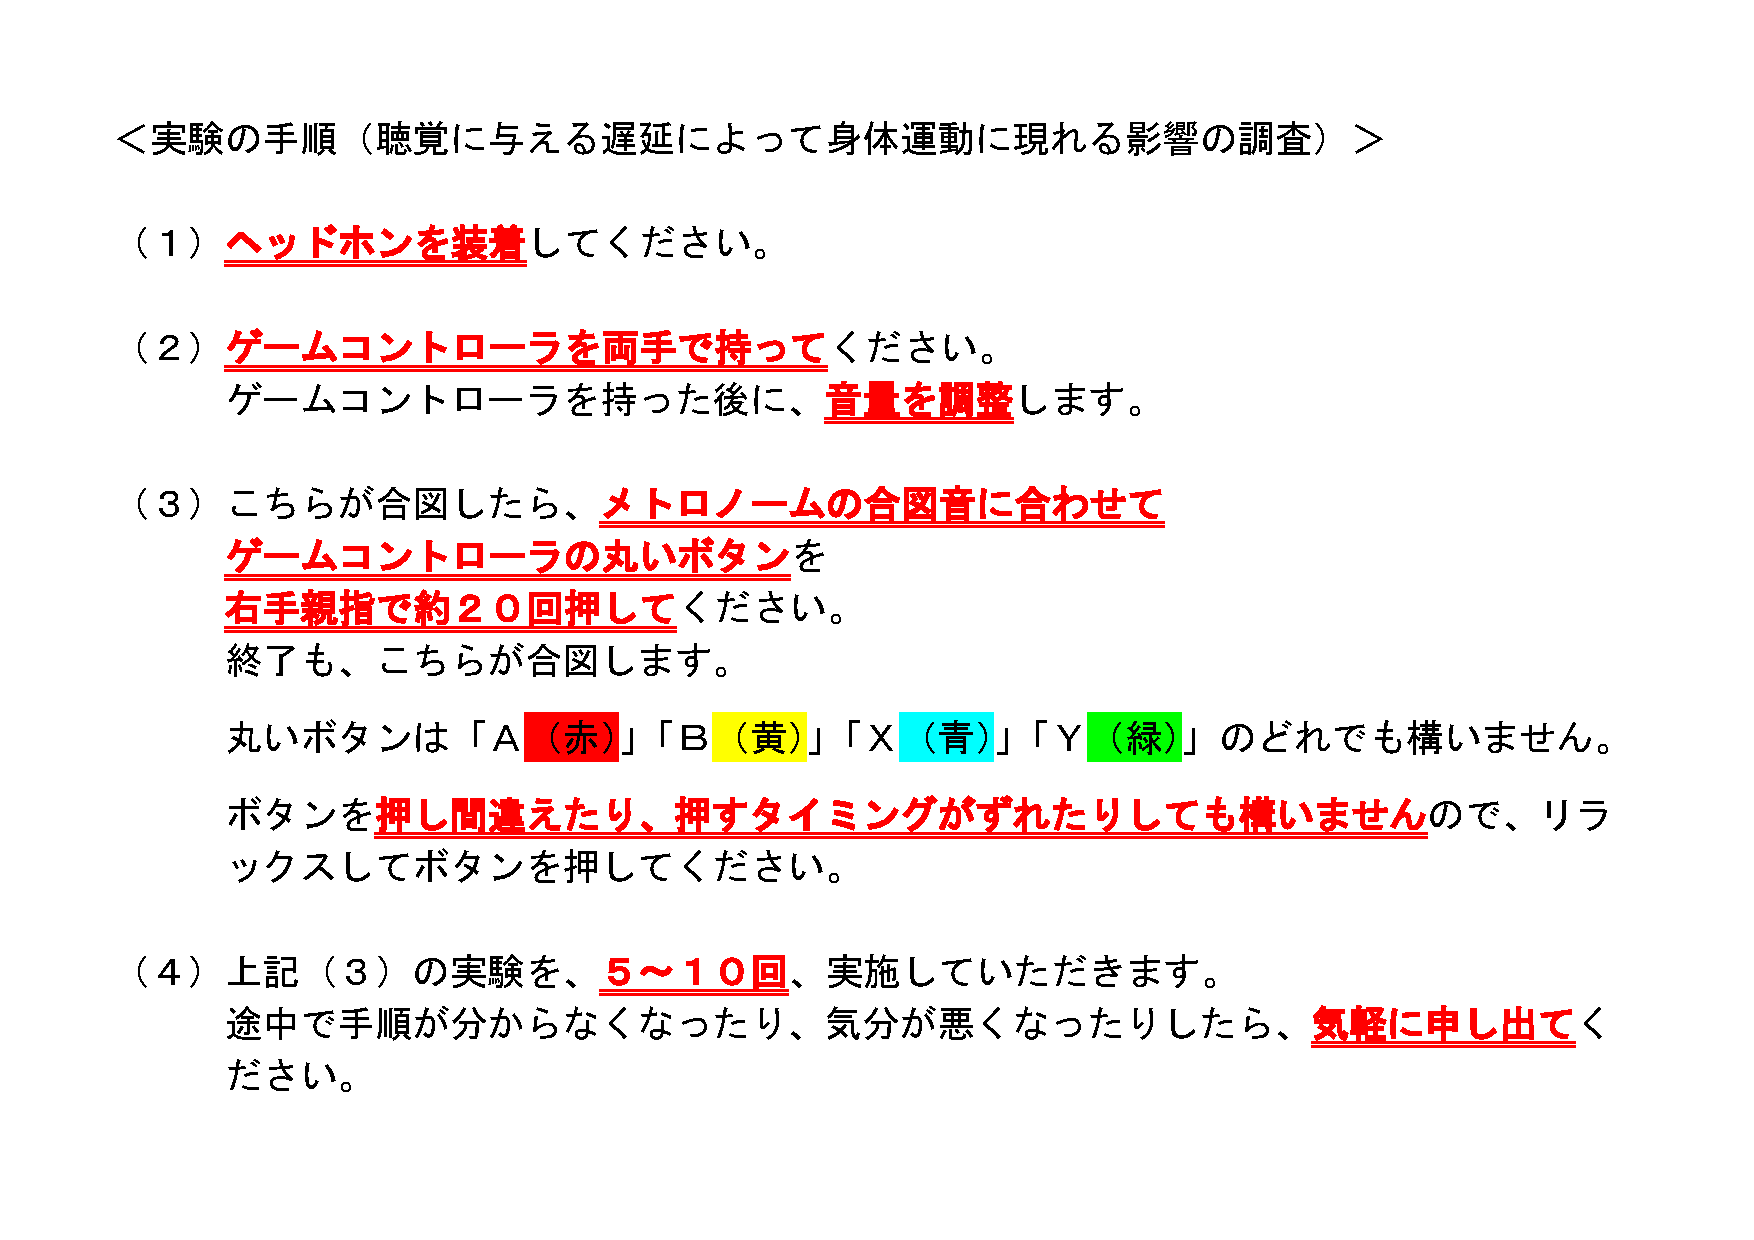
\includegraphics[scale=0.4]{furoku_A/Less60_Tezyunn.pdf}
  \caption{実験手順説明ボード(60歳未満の方用)}
\end{figure}
\begin{figure}[ht]
  \centering
  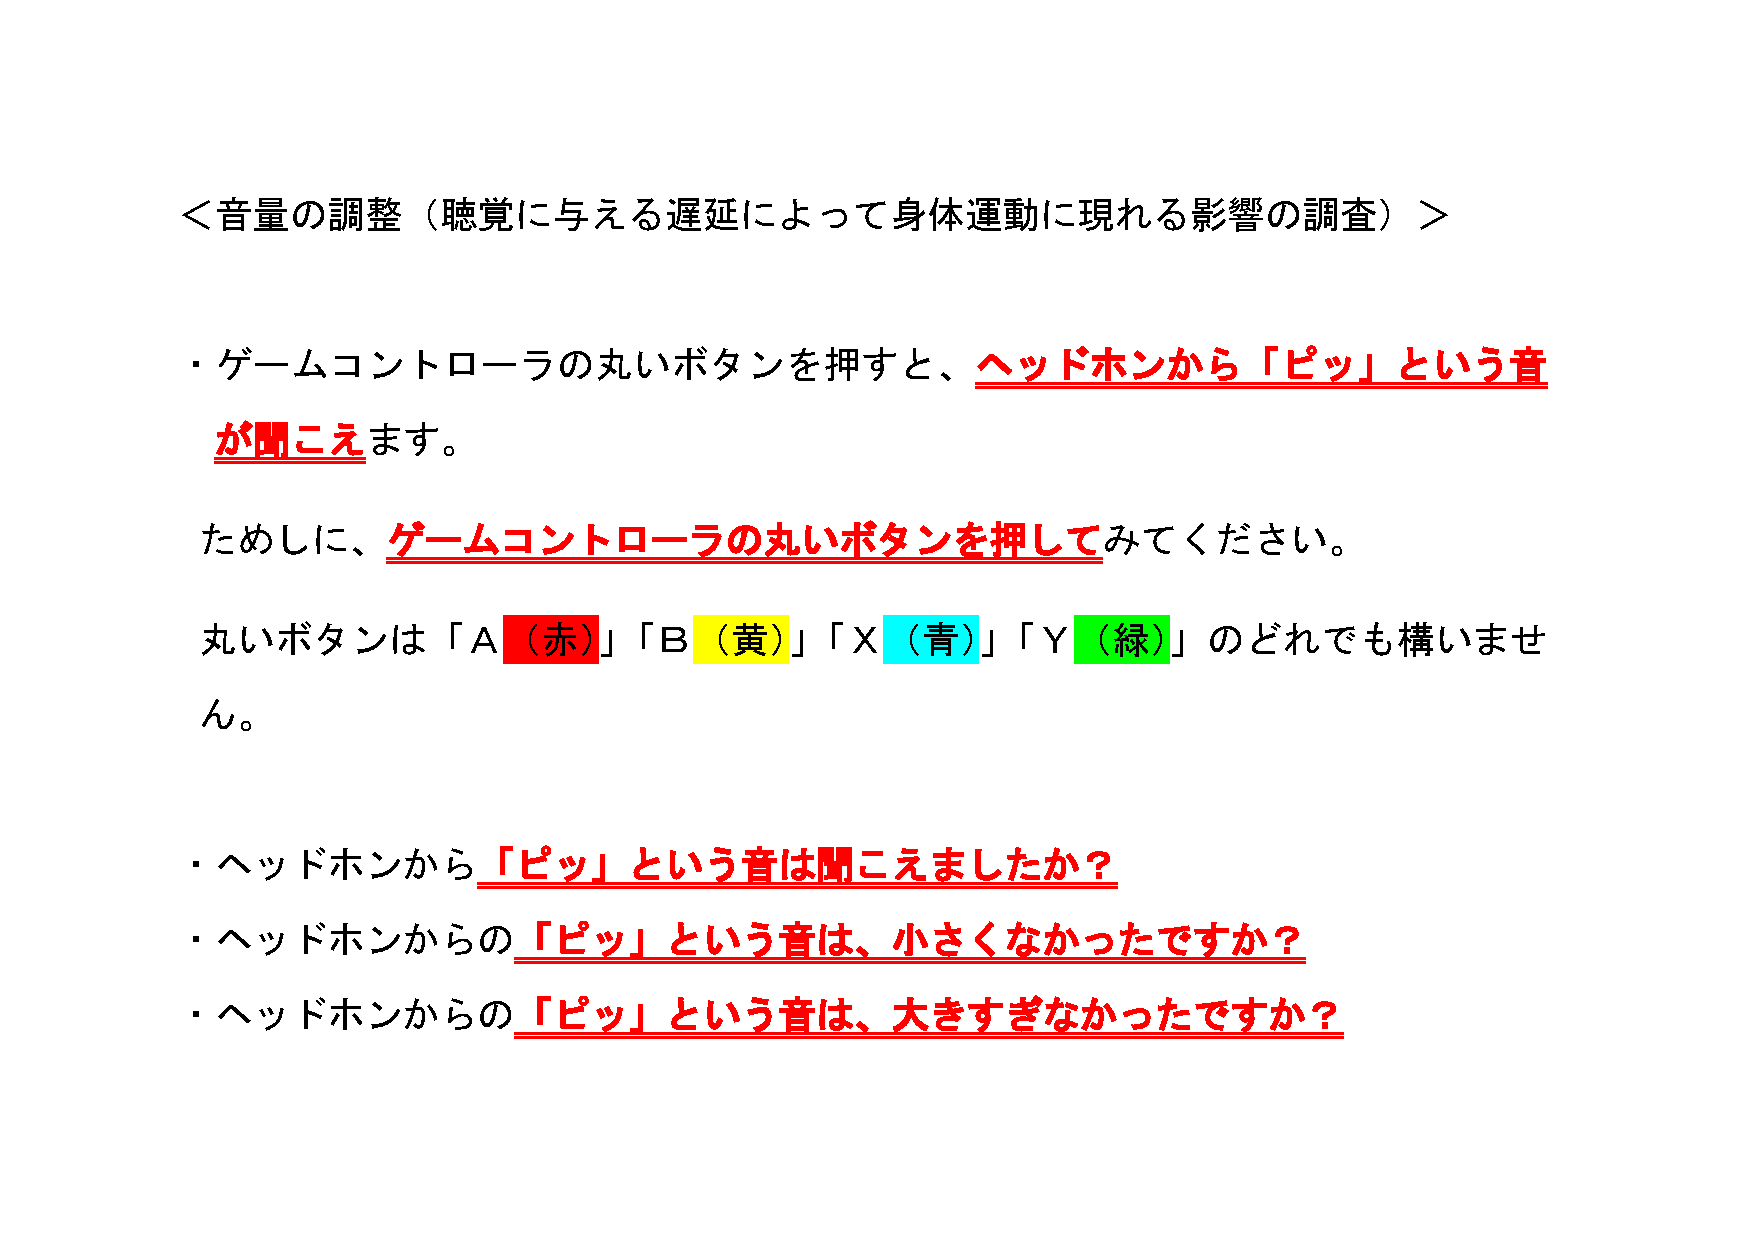
\includegraphics[scale=0.4]{furoku_A/Onnryou.pdf}
  \caption{音量調整ボード}
\end{figure}
%%%%%%%%%%%%%%%%%%%%%%%%%%%%%%%%%%%%%%%%%%%%%%%%%%%%%%%%%%%%%%%%%
% 付録B
%%%%%%%%%%%%%%%%%%%%%%%%%%%%%%%%%%%%%%%%%%%%%%%%%%%%%%%%%%%%%%%%%
\chapter{主観調査におけるアプリケーションのソースコード}
% 開発した主観調査におけるアプリケーションを掲載する.本プログラムは,Microsoft Visual Studio 2022でコンパイルできるソースファイル,ヘッダファイルおよびリソースファイルである.関数の目的別にファイルを分けて作成している.

% \begin{lstlisting}[caption=main.cpp]
% //////////////////////////////////////////
% // main.cpp: WinMain関数・ウィンドウプロージャの定義
% //////////////////////////////////////////

% #include<windows.h>
% #include<stdio.h>
% #include<tchar.h>
% #include<WinUser.h>
% #include<commctrl.h> 
% #include<random>
% #include<string>
% #include<iomanip>
% #include<stdlib.h>
% #include<windowsx.h>
% #include<manipulations.h> // Touch Input用

% /////////////////////////////////////
% /// 自作ヘッダファイルのインクルード
% /////////////////////////////////////
% #include"main.h"
% #include"window.h"
% #include"resource.h"
% #include"file.h"
% #include"UserInfoWindow.h"

% using namespace std;

% /////////
% // pragma
% // 1.コモンコントロール
% // 2.音声再生用
% // 3.ビジュアルスタイルの有効化
% /////////
% #pragma comment(lib, "comctl32.lib")
% #pragma comment(lib, "winmm.lib")
% #pragma comment(linker,"/manifestdependency:\"type='win32' \
%   name='Microsoft.Windows.Common-Controls' \
%   version='6.0.0.0' \
%   processorArchitecture='*' \
%   publicKeyToken='6595b64144ccf1df' \
%   language='*'\"") 

% ///////////
% // 定数
% ///////////
% #define STRLEN 256   // 文字列の最大長
% #define GetMonitorRect(rc)  SystemParametersInfo(SPI_GETWORKAREA,0,rc,0)  // ワークエリア領域の取得
% #define CONBOMAX9 9  // コンボボックスの項目数(Group1~5)
% #define CONBOMAX8 8  // コンボボックスの項目数(Group6~10)
% #define LENSNUMBER 128


% //////////////////////////////
% //グローバル変数の宣言・初期化
% /////////////////////////////
% const char	szWinName[5] = _T("Test");
% static const char   szWinName2[] = _T("テスト");
% HINSTANCE hInst;
% HWND hDlg;
% extern char WindowTitleText[32];
% extern int intCurrentIndex;

% //ButtonEnableFunc()で利用
% bool boolstart;  // true: 「ウィンドウが生成されてから1回以上次へボタンを押した」 false: 「ウィンドウが生成されてからまだ次へボタンを押していない」
% bool ZeroOrNot;  // true: 「変数NumberOfTimesが0である」 false: 「変数NumberOfTimesが0以外である」

% // ファイルに書き込んだか否かの取得
% bool FileWriteInfo;

% //HWND hChildUserInfo;

% // 背景
% extern const HBRUSH BackGround_clear = CreateSolidBrush(RGB(235, 235, 235));
% extern const COLORREF TextBackground = RGB(235, 235, 235);
% const COLORREF ColorEdgeButton = RGB(100, 149, 237);

% // フォントサイズ
% extern int fontsize;   // エディットボックスのフォント
% extern int fontsize2;

% // その他変数
% extern unsigned int NumberOfTimes;          // 実験回数を保持する変数
% char Grade[STRLEN];                      // 評価結果の保存用変数
% extern char GradeSpeak[STRLEN],GradeLate[STRLEN];
% HANDLE hfile;
% extern unsigned int GradeS[STRLEN], GradeL[STRLEN];

% char Result[STRLEN];              // 全評価結果を保持する変数
% short int IndexResult;            // Result[]のインデックス番号 
% extern short int i;               // 評価結果保存用配列のインデックス番号
% extern char temp1[STRLEN];
% char temp3[STRLEN];

% // 読み上げる文章の順番を決めるための操作
% extern int SNumber[LENSNUMBER];
% int* P_SNumber;

% // 座標
% int key_i[2] = { 30, 170 };         
% int NumberTest_i[2] = { 40, 215 };  // 表示させる実験回数の座標

% // ファイルへの出力用変数
% DWORD dwWriteSize;


% // コンボボックス内
% int intTxtLen;
% char* pszBuf;

% ////////////////////
% // RECT構造体変数
% ///////////////////
 
% extern RECT FrameTop, FrameProgTop, FrameCenter;
% extern RECT Frame1;
% extern RECT Frame2;
% extern RECT Frame3;
% extern RECT FrameUserInfo;
% extern RECT FrameComment;
% extern RECT FrameProg;
% extern RECT RectButton1, RectButton2, RectButton3, RectButton4, RectButton11, RectButton22, RectButton33, RectButton44;
% RECT Frame4 = { 30, FrameTop.top + 20 - 2, FrameTop.left + 600 + 2, FrameTop.top + 20 + fontsize + 3+2 , };
% RECT Frame5 = { FrameTop.left - 2, 130 - 2, FrameTop.left + 70+ 2, 130 + fontsize + 3+2 };
% RECT Frame_ReadNumber = { Winsize.left + 30, Frame1.top, Winsize.right - 30 / 2, Frame1.bottom };

% /////////////////////////
% // 子ウィンドウのハンドル
% /////////////////////////
% extern HWND Button1, Button2, Button3, Button4, Button11, Button22, Button33, Button44;
% extern HWND hStaticProg, hStaticProg2, hNumberStatic, latedatacombo, hStaticUserDialog, hDialogUser, hStaticSentence;


% HPEN hpen;
% HBRUSH hbr;
% HFONT hFont1;
% HDC hdc;
% /////////////////////////////////////////
% // プログレスバーで使用するグローバル変数
% /////////////////////////////////////////
% int  _MAX, _MIN, _POS, _TEMP;              // プログレスバーで利用する変数
% char bufferProg[10];                           // ステティックコントロールに設定する文字列を格納
% bool TempMAX;
% bool TempResult = true;

% // メモリデバイスコンテキスト
% HDC  hDCMem, hDCMem4;
% HGDIOBJ hDCMemOld, hDCMemOld4;

% // OwnerDrawButton用
% int selectedButtonID_1 = -1;
% int selectedButtonID_2 = -1;
% bool bBtn1 = false;
% bool bBtn2 = false;
% bool bBtn3 = false;
% bool bBtn4 = false;
% bool bBtn5 = false;
% bool bBtn6 = false;
% bool bBtn7 = false;
% bool bBtn8 = false;

% COLORREF color_Buttonbackground = RGB(73, 135, 242);
% COLORREF color_iniButtonbackground = RGB(218,227,242);
% char szText[50];
% bool ButtonBool = false;
% bool Clicked_1 = false;
% bool Clicked_2 = false;
% /*----------------------------------------------------------------------------------------------------------------------*/
% ////////////////////
% //WinMain関数の定義
% ////////////////////
% int APIENTRY WinMain(_In_ HINSTANCE hThisInst, _In_opt_ HINSTANCE hPrevInst, _In_ LPSTR lpszArgs, _In_ int nWinMode)
% {
% 	HWND		hWnd = NULL;
% 	HWND        hWndNew = NULL;
% 	MSG			uMsg;
	
% 	// クライアント領域のサイズ調整
% 	AdjustWindowRectEx(&Winsize, WS_OVERLAPPEDWINDOW, true, 0);

% 	// Show First Window
% 	CreateNewWindow(hWndNew, hThisInst, Winsize.right - Winsize.left, Winsize.bottom - Winsize.top, nWinMode);

% 	//インスタンスハンドルの保存
% 	hInst = hThisInst;

% 	//メッセージループの生成
% 	while (GetMessage(&uMsg, NULL, 0, 0)) {
% 		// GetMessage()関数の戻り値が0になったら(WM_QUITを受け取ったら)ループを抜ける
% 		TranslateMessage(&uMsg);
% 		DispatchMessage(&uMsg);
% 	}
% 	return((int)uMsg.wParam);
% }

% //////////////////////////////////////
% // ウィンドウプロージャの定義
% //////////////////////////////////////
% LRESULT CALLBACK WndProc(HWND hWnd, UINT uMsg, WPARAM wParam, LPARAM lParam)
% {
% 	short int IGrade;                       
% 	INITCOMMONCONTROLSEX initctrl;      // INITCOMMONCONTROLSEX 構造体変数
% 	PAINTSTRUCT ps;
% 	//HWND hwndButton;
	

% 	switch (uMsg){
% 		//終了処理
% 	case WM_DESTROY:
% 		// 書き込み済みの場合は書き込まない
% 		if (!FileWriteInfo) {
% 			// ファイルのオープン
% 			file_open(hWnd);
% 			// ファイルへの書き込み
% 			WriteFileFunc();
% 			// ファイルのクローズ
% 			CloseHandle(hfile);
% 		}
% 		// 後始末
% 		DeleteObject(hFont);
% 		DeleteObject(hFont1);
% 		DeleteObject(hFont2);
% 		DeleteObject(hFontTitle);
% 		DeleteObject(hpen);
% 		DeleteObject(hbr);
% 		SelectObject(hDCMem, hDCMemOld);
% 		SelectObject(hDCMem4, hDCMemOld4);
% 		DeleteDC(hDCMem);
% 		DeleteDC(hDCMem4);
		
% 		//DeleteObject(hBrush); // オーナードローボタンで使用

% 		// WM_QUITをメッセージキューにポスト
% 		PostQuitMessage(0);
% 		return 0;

% 	case WM_CREATE:
% 		P_SNumber = SNumber;                         // 読み上げる文章の番号を格納する配列

% 		// INITCOMMONCONTROLSEX 構造体の初期化
% 		memset(&initctrl, 0, sizeof(initctrl));
% 		initctrl.dwSize = sizeof(initctrl); // INITCOMMONCONTROLSEX構造体のサイズ
% 		initctrl.dwICC = ICC_WIN95_CLASSES; // コモンコントロールクラスの指定(プログレスバー)
% 		InitCommonControlsEx(&initctrl);    // 使用するコントロールクラスの登録

% 		// 画面中央にウィンドウを移動
% 		DesktopCenterWindow(hWnd);

% 		// 初期化処理
% 		WM_CREATE_Func(hWnd, lParam);
	
% 		break;

% 	case WM_CTLCOLORSTATIC:
% 		return (SetCtlColor(wParam, lParam));
	
% 	case WM_TOUCH:
% 		OnTouch(hWnd, wParam, lParam);
% 		break;


% 	case WM_PAINT:
% 	{
% 		hdc = BeginPaint(hWnd, &ps);
% 		// メモリDCからDCへコピー
% 		BitBlt(ps.hdc,
% 			ps.rcPaint.left, ps.rcPaint.top,
% 			ps.rcPaint.right - ps.rcPaint.left, ps.rcPaint.bottom - ps.rcPaint.top,
% 			hDCMem,
% 			ps.rcPaint.left, ps.rcPaint.top,
% 			SRCCOPY);

% 		// ビットマップ画像
% 		BitBlt(ps.hdc,
% 			110, 90,
% 			ps.rcPaint.right - ps.rcPaint.left, ps.rcPaint.bottom - ps.rcPaint.top,
% 			hDCMem4,
% 			0, 0, SRCCOPY);

% 		RECT rc;
% 		GetClientRect(hWnd, &rc);
% 		int x = rc.right - rc.left;
% 		int y = rc.bottom - rc.top;
		
% 		EndPaint(hWnd, &ps);

% 	}
% 		return 0;

% 	case WM_ERASEBKGND:
% 		// 何も処理しない(画面のちらつき防止)
% 		return 1;
% 		break;

% 	case WM_COMMAND:
% 		CommandFunc(hWnd, wParam, lParam, uMsg, hdc);
% 		break;

% 	case WM_DRAWITEM:
% 	{
% 		LPDRAWITEMSTRUCT pdis = (LPDRAWITEMSTRUCT)lParam;
	
% 		switch(pdis->CtlID)
% 		{
% 		case ID_BUTTON1:
% 			OnDrawItem(bBtn1, pdis->hDC, pdis->rcItem, pdis->hwndItem);
% 			break;

% 		case ID_BUTTON2:
% 			OnDrawItem(bBtn2, pdis->hDC, pdis->rcItem, pdis->hwndItem);
% 			break;

% 		case ID_BUTTON3:
% 			OnDrawItem(bBtn3, pdis->hDC, pdis->rcItem, pdis->hwndItem);
% 			break;

% 		case ID_BUTTON4:
% 			OnDrawItem(bBtn4, pdis->hDC, pdis->rcItem, pdis->hwndItem);
% 			break;

% 		case ID_BUTTON11:
% 			OnDrawItem(bBtn5, pdis->hDC, pdis->rcItem, pdis->hwndItem);
% 			break;

% 		case ID_BUTTON22:
% 			OnDrawItem(bBtn6, pdis->hDC, pdis->rcItem, pdis->hwndItem);
% 			break;

% 		case ID_BUTTON33:
% 			OnDrawItem(bBtn7, pdis->hDC, pdis->rcItem, pdis->hwndItem);
% 			break;

% 		case ID_BUTTON44:
% 			OnDrawItem(bBtn8, pdis->hDC, pdis->rcItem, pdis->hwndItem);
% 			break;

% 		default:
% 			return(TRUE);
% 		}
% 	}
% 	return(TRUE);

% 	case WM_CHAR:
% 		switch (wParam) {
% 		case VK_ESCAPE:
% 			PostQuitMessage(0);
% 			break;

% 		case '1':
% 			//PlaySound(TEXT("whistle.wav"), NULL, SND_FILENAME);
% 			// 入力キーの保存
% 			IGrade = 1;
% 			Grade[i] = '1';
% 			i++;
% 			// 実験回数の更新
% 			NumberOfTimes++;
% 			CountNumberFunc(NumberOfTimes);
% 			break;

% 		case '2':
% 			//PlaySound(TEXT("summernight.wav"), NULL, SND_FILENAME);
% 			// 入力キーの保存
% 			IGrade = 2;
% 			Grade[i] = '2';
% 			i++;
% 			//実験回数の更新と表示
% 			NumberOfTimes++;
% 			CountNumberFunc(NumberOfTimes);
% 			break;

% 		case '3':
% 			// 入力キーの保存
% 			IGrade = 3;
% 			Grade[i] = '3';
% 			i++;
% 			//実験回数の更新と表示
% 			NumberOfTimes++;
% 			CountNumberFunc(NumberOfTimes);
% 			break;

% 		case '4':
% 			// 入力キーの保存
% 			IGrade = 4;
% 			Grade[i] = '4';
% 			i++;
% 			// 実験回数の更新と表示
% 			NumberOfTimes++;
% 			CountNumberFunc(NumberOfTimes);
% 			break;

% 		case 0x08: // バックスペース
% 			NumberOfTimes--;                        // 入力回数の更新
% 			hdc = GetDC(hWnd);
% 			CancelFunc(hWnd, hdc, NumberOfTimes);
% 			SetNumber(P_SNumber, NumberOfTimes); // 文章の番号の決定
% 			DispNumberSentence(hdc);                    // 文章の番号の表示
% 			ReleaseDC(hWnd, hdc);
% 			break;

% 		default:
% 			MessageBox(hWnd, "1, 2, 3, 4いずれかのキーを押してください。", NULL, MB_OK | MB_ICONWARNING);
% 			break;
% 		}
% 		return 0;

% 	case WM_KEYUP:
% 		// 何らかのキーが押されたときに発生するイベント
% 		break;

% 	case WM_KEYDOWN:
% 		switch (wParam) {
% 			// Enterを押すと
% 		case VK_RETURN:
% 			// 出力先ファイルが既に開かれていたとき、注意
% 			//WarningFileOpen(hWnd);
% 			if (MessageBox(hWnd, "終了しますか?", "終了確認", MB_YESNO | MB_ICONQUESTION) == IDYES) {
% 				DestroyWindow(hWnd);
% 			}
% 			return 0;
% 		}
% 		break;
 
% 	case WM_CLOSE:
% 		// 出力先ファイルが既に開かれていたとき、注意
% 		//WarningFileOpen(hWnd);
% 		if (MessageBox(hWnd, (LPCSTR)"終了しますか?", (LPCSTR)"終了確認", MB_YESNO | MB_ICONQUESTION) == IDYES) {
% 			DestroyWindow(hWnd);
% 		}
% 		break;

% 	default:
% 		// ボタンの有効・無効の切り替え
% 		ButtonEnableFunc();
% 		return (DefWindowProc(hWnd, uMsg, wParam, lParam));
	
% 	}
% 	return(0);  
% }


% /////////////////////
% // オーナーボタンの描画
% /////////////////////
% bool OnDrawItem(bool bBtn, HDC hDC, RECT rcItem, HWND hwndItem) {

% 	HBRUSH hBrush_ini = (HBRUSH)CreateSolidBrush(color_iniButtonbackground);
% 	HBRUSH hBrush = CreateSolidBrush(RGB(73, 135, 242));

% 	FillRect(hDC, &rcItem, hBrush_ini);
% 	DrawEdge(hDC, &rcItem, EDGE_RAISED, BF_RECT);
% 	GetWindowText(hwndItem, szText, 50);
% 	// Draw Text on Button
% 	SetTextColor(hDC, RGB(0, 0, 0));
% 	SetBkColor(hDC, color_iniButtonbackground);
% 	DrawText(hDC, szText, -1, &rcItem, DT_CENTER | DT_VCENTER | DT_SINGLELINE);

% 	if (bBtn) {
% 		FillRect(hDC, &rcItem, hBrush);
% 		DrawEdge(hDC, &rcItem, EDGE_SUNKEN, BF_RECT);
% 		GetWindowText(hwndItem, szText, 50);
% 		// Draw Text on Button
% 		SetTextColor(hDC, RGB(255, 255, 255));
% 		SetBkColor(hDC, color_Buttonbackground);
% 		DrawText(hDC, szText, -1, &rcItem, DT_CENTER | DT_VCENTER | DT_SINGLELINE);
% 	}

% 	// clean object
% 	DeleteObject(hBrush_ini);
% 	DeleteObject(hBrush);

% 	return true;
% }

% /////////////////////////
% // ボタンの有効化・無効化
% /////////////////////////
% bool ButtonEnableFunc() {

% 	// ボタンの有効化
% 	if (!boolstart) {
% 		 //一度有効化したら終了まで有効状態
% 		if (strMenLady) {
% 			EnableWindow(hReserch, TRUE);
% 			boolstart = true;
% 		}
% 	}
% 	else if (!ZeroOrNot) {
% 		if (NumberOfTimes > 0) {
% 			EnableWindow(hCancel, TRUE);
% 			// 一度有効化したら次に無効状態になるまで有効化しない
% 			ZeroOrNot = true;
% 		}
% 	}
% 	else if ((NumberOfTimes == 0)) {
% 		// 0になったら無効化する
% 		EnableWindow(hCancel, FALSE);
% 		ZeroOrNot = false;
% 	}
% 	else if(NumberOfTimes == _MAX * 2){
% 		// 終了後にボタンを無効化
% 		EnableWindow(hCancel, FALSE);
% 		EnableWindow(Button1, FALSE);
% 		EnableWindow(Button2, FALSE);
% 		EnableWindow(Button3, FALSE);
% 		EnableWindow(Button4, FALSE);
% 		EnableWindow(Button11, FALSE);
% 		EnableWindow(Button22, FALSE);
% 		EnableWindow(Button33, FALSE);
% 		EnableWindow(Button44, FALSE);
% 		EnableWindow(hReserch, FALSE);
% 		EnableWindow(hNext, FALSE);
% 	}
% 	return true;
% }

% //////////////////////////////
% // WM_CREATEメッセージの定義
% //////////////////////////////
% bool WM_CREATE_Func(HWND hWnd, LPARAM lParam) {
% 	// グローバル変数の初期化
% 	NumberOfTimes = 0;                    // 実験回数を保存する変数
% 	i = 0;                                // 評価結果を保存する配列のインデックス
% 	// 子ウィンドウ作成
% 	//ComboboxFunc(hWnd, lParam);           // 遅延時間設定用
% 	ReserchStartFunc(hWnd, lParam);       // 実験開始ボタン
% 	CreateOwnerDrawButton(hWnd, lParam);  // 評価結果入力用ボタン
% 	CreateProgressBar(hWnd, 40, lParam);  // プログレスバーの作成
% 	//プログレスバーの設定
% 	ChangeProgBarMAX(intCurrentIndex);
% 	// 読み上げる文章の順番を決定									  
% 	Getarray(P_SNumber, 10);
% 	// メモリデバイスコンテキスト描画の事前準備
% 	GetWindowMemDCFunc(hWnd);
% 	// メモリデバイスコンテキストへの描画
% 	PaintFunc(hWnd);
% 	// フォントの適用
% 	FontFunc();                        
% 	return true;

% }

% //////////////////////////////////////////////////
% // メモリデバイスコンテキスト描画の事前準備
% //////////////////////////////////////////////////
% bool GetWindowMemDCFunc(HWND hWnd) {

% 	HDC hDC;
% 	HBITMAP hBitmap, hBitmap4;
% 	BITMAP bitmap4{};
	
% 	//デバイスコンテキストの取得
% 	hDC = GetDC(hWnd);
% 	// メモリデバイスコンテキストの取得
% 	hDCMem = CreateCompatibleDC(hDC);
% 	hDCMem4 = CreateCompatibleDC(hDC);
% 	// ビットマップハンドルの取得
% 	hBitmap = CreateCompatibleBitmap(hDC, Winsize.right, Winsize.bottom);
% 	hBitmap4 = LoadBitmap(GetModuleHandle(NULL),//(HINSTANCE)GetWindowLongPtr(hWnd, GWL_HINSTANCE),
% 		MAKEINTRESOURCE(IDB_BITMAP3));
% 	// ビットマップ画像のサイズ取得
% 	GetObject(hBitmap4, sizeof(BITMAP), &bitmap4);
% 	// デバイスコンテキストの解放(メモリデバイスコンテキストを取得するためだけに使うからもう不要)
% 	ReleaseDC(hWnd, hDC);
% 	// メモリDCにビットマップを割りつけ
% 	hDCMemOld = SelectObject(hDCMem, hBitmap);
% 	hDCMemOld4 = SelectObject(hDCMem4, hBitmap4);
% 	// ビットマップの削除(ビットマップはメモリデバイスコンテキストの情報を設定するためだけに使うからもう不要)
% 	DeleteObject(hBitmap);
% 	DeleteObject(hBitmap4);

% 	return true;
% }

% //////////////////////////////////////////
% // メモリデバイスコンテキストへの描画
% //////////////////////////////////////////
% bool PaintFunc(HWND hWnd) {

% 	HRGN hRgn;// , hRgn1, hRgn2, hRgn3;

% 	// フォントの定義
% 	hFont1 = CreateFont(
% 		fontsize2, 0, 0, 0,
% 		FW_MEDIUM,
% 		false, false, false,
% 		SHIFTJIS_CHARSET, OUT_DEFAULT_PRECIS,
% 		CLIP_DEFAULT_PRECIS, DEFAULT_QUALITY,
% 		(VARIABLE_PITCH | FF_DONTCARE), _T("メイリオ"));
% 	//
% 	// ウィンドウの背景の設定
% 	hRgn = CreateRectRgn(Winsize.left, Winsize.top, Winsize.right, Winsize.bottom);
% 	FillRgn(hDCMem, hRgn, (HBRUSH)CreateSolidBrush(RGB(255,255,255)));
% 	FillRect(hDCMem, &FrameProgTop, (HBRUSH)CreateSolidBrush(RGB(70, 130, 180)));
% 	FillRect(hDCMem, &FrameBottom, (HBRUSH)CreateSolidBrush(RGB(70, 130, 180)));
% 	FillRect(hDCMem, &FrameCenter, BackGround_clear);
% 	/*hRgn1 = CreateRectRgn(FrameBottom.left - 30, FrameBottom.bottom - 64, FrameBottom.right + 30, FrameBottom.bottom);
% 	hRgn2 = CreateRectRgn(0, 0, 30, Winsize.bottom - (FrameBottom.bottom - FrameBottom.top + 5));
% 	hRgn3 = CreateRectRgn(Winsize.right - 30, 0, Winsize.right, Winsize.bottom - (FrameBottom.bottom - FrameBottom.top + 5));*/
% 	//FillRgn(hDCMem, hRgn1, (HBRUSH)CreateSolidBrush(RGB(155,169,194)));
% 	/*FillRgn(hDCMem, hRgn2, (HBRUSH)CreateSolidBrush(RGB(22, 33, 77)));
% 	FillRgn(hDCMem, hRgn3, (HBRUSH)CreateSolidBrush(RGB(22, 33, 77)));*/
% 	DeleteObject(hRgn);
% 	//DeleteObject(hRgn1);
% 	/*DeleteObject(hRgn2);
% 	DeleteObject(hRgn3);*/
% 	// 文字列の背景の設定
% 	SetBkColor(hDCMem, TextBackground);
% 	// フォントの適用
% 	SelectObject(hDCMem, hFont1);
	
% 	// 枠線
% 	DrawEdge(hdc, &FrameBottom, EDGE_RAISED, BF_TOP);

% 	return true;
% }
% ///////////////////////////////
% // WM_COMMANDメッセージの定義
% ///////////////////////////////
% bool CommandFunc(HWND hWnd, WPARAM wParam, LPARAM lParam, UINT uMsg, HDC hdc) {

% 	int MsgResult;
	
% 	switch (LOWORD(wParam)){
% 	case ID_BUTTON1:
% 		GradeS[i] = 1;
% 		Clicked_1 = true;
% 		bBtn1 = true;
% 		bBtn2 = false;
% 		bBtn3 = false;
% 		bBtn4 = false;
% 		InvalidateRect(hWnd, &FrameCenter, FALSE);
% 		//SendMessage(hWnd, WM_DRAWITEM, (WPARAM)0, (LPARAM)&dis);
% 		break;

% 	case ID_BUTTON2:
% 		GradeS[i] = 2;
% 		Clicked_1 = true;
% 		bBtn1 = false;
% 		bBtn2 = true;
% 		bBtn3 = false;
% 		bBtn4 = false;
% 		InvalidateRect(hWnd, &FrameCenter, TRUE);
% 		break;

% 	case ID_BUTTON3:
% 		GradeS[i] = 3;
% 		Clicked_1 = true;
% 		bBtn1 = false;
% 		bBtn2 = false;
% 		bBtn3 = true;
% 		bBtn4 = false;
% 		InvalidateRect(hWnd, &FrameCenter, TRUE);
% 		break;

% 	case ID_BUTTON4:
% 		GradeS[i] = 4;
% 		Clicked_1 = true;
% 		bBtn1 = false;
% 		bBtn2 = false;
% 		bBtn3 = false;
% 		bBtn4 = true;
% 		InvalidateRect(hWnd, &FrameCenter, TRUE);
% 		break;

% 	case ID_BUTTON11:
% 		GradeL[i] = 1;
% 		Clicked_2 = true;
% 		bBtn5 = true;
% 		bBtn6 = false;
% 		bBtn7 = false;
% 		bBtn8 = false;
% 		InvalidateRect(hWnd, &FrameCenter, TRUE);
% 		break;

% 	case ID_BUTTON22:
% 		GradeL[i] = 2;
% 		Clicked_2 = true;
% 		bBtn5 = false;
% 		bBtn6 = true;
% 		bBtn7 = false;
% 		bBtn8 = false;
% 		InvalidateRect(hWnd, &FrameCenter, TRUE);
% 		break;

% 	case ID_BUTTON33:
% 		GradeL[i] = 3;
% 		Clicked_2 = true;
% 		bBtn5 = false;
% 		bBtn6 = false;
% 		bBtn7 = true;
% 		bBtn8 = false;
% 		InvalidateRect(hWnd, &FrameCenter, TRUE);
% 		break;

% 	case ID_BUTTON44:
% 		GradeL[i] = 4;
% 		Clicked_2 = true;
% 		bBtn5 = false;
% 		bBtn6 = false;
% 		bBtn7 = false;
% 		bBtn8 = true;
% 		InvalidateRect(hWnd, &FrameCenter, TRUE);
% 		break;
		
% 	break;

% 	case ID_LATEINI:
% 		LateIniFunc(hWnd, wParam);
% 		break;

	
% 	case ID_ReserchStart:
% 		if (HIWORD(wParam) == BN_CLICKED) {
% 			SetFocus(hWnd);    // 親ウィンドウへフォーカスを移動
% 			// ボタンの有効化
% 			EnableWindow(hNext, TRUE);
% 			EnableWindow(Button1, TRUE);
% 			EnableWindow(Button2, TRUE);
% 			EnableWindow(Button3, TRUE);
% 			EnableWindow(Button4, TRUE);
% 			EnableWindow(Button11, TRUE);
% 			EnableWindow(Button22, TRUE);
% 			EnableWindow(Button33, TRUE);
% 			EnableWindow(Button44, TRUE);
% 			// 遅延時間設定用コンボボックスの無効化
% 			EnableWindow(latedatacombo, false);
% 			MessageBox(hWnd, _T("調査を開始します。"), _T("開始確認"), MB_OK);
% 			// 読み上げる文章の番号を計算し、表示
% 			SetNumber(P_SNumber, NumberOfTimes);
% 			DispNumberSentence(hDCMem);
% 		}
		
% 		break;
    
% 	case ID_NEXTBUTTON:
% 		if (HIWORD(wParam) == BN_CLICKED) {
% 			if (TempMAX) {
% 				MsgResult = MessageBox(hWnd, _T("これで調査は終了です。終了ボタンを押しウィンドウを閉じてください。"), _T("調査終了確認"), MB_OKCANCEL);
% 				if ( MsgResult == IDCANCEL) {
% 					break;
% 				}
% 				else if (MsgResult == IDOK){
% 					hdc = GetDC(hWnd);
% 					NextButtonFunc(hWnd, hdc);
% 					// プログレスバーを更新する
% 					_TEMP = SendMessage(hProg, PBM_STEPIT, 0, 0);
% 					//現在値を取得
% 					_POS = SendMessage(hProg, PBM_GETPOS, 0, 0);
% 					//最大値を超えない場合は1ステップ&テキストに現在値を設定
% 					if (_POS <= _MAX) {
% 						wsprintf(bufferProg, "%d / %d", _POS, _MAX);
% 						SendMessage(hStaticProg, WM_SETTEXT, 0, (LPARAM)bufferProg);
% 						if (_POS == _MAX) {
% 							TempMAX = true;
% 						}
% 					}
% 					const char* bufferSentence = _T("ありがとうございました。");
% 					SendMessage(hStaticSentence, WM_SETTEXT, 0, (LPARAM)bufferSentence);
% 					/////////////////////////
% 					// ファイルに結果を出力
% 					/////////////////////////
% 					file_open(hWnd);          // テキストファイルのオープン
% 					WriteFileFunc();      // ファイルへの書き込み
% 					CloseHandle(hfile);   // ファイルのクローズ
% 					FileWriteInfo = true; // ファイルに書き込み済みであることを知らせる(WM_DESTROYで使用)
% 					break;
					
% 				}
					
% 			}
% 			else {
% 				hdc = GetDC(hWnd);
% 				NextButtonFunc(hWnd, hdc);
% 				if (!TempResult) {
% 					// 正しく回答できていないときは何もしない
% 					break;
% 				}
% 				// プログレスバーを更新する
% 				_TEMP = SendMessage(hProg, PBM_STEPIT, 0, 0);
% 				//現在値を取得
% 				_POS = SendMessage(hProg, PBM_GETPOS, 0, 0);
% 				//最大値を超えない場合は1ステップ&テキストに現在値を設定
% 				if (_POS <= _MAX) {
% 					wsprintf(bufferProg, _T("%d / %d"), _POS, _MAX);
% 					SendMessage(hStaticProg, WM_SETTEXT, 0, (LPARAM)bufferProg);
% 					if (_POS == _MAX) {
% 						TempMAX = true;
% 					}
% 				}
% 				ReleaseDC(hWnd, hdc);
% 				SetFocus(hWnd);
% 			}
% 		}
% 		break;


% 	case ID_CANCEL:
% 		if (HIWORD(wParam) == BN_CLICKED) {
% 			hdc = GetDC(hWnd);
% 			NumberOfTimes = CancelFunc(hWnd, hdc, NumberOfTimes);
% 			SetNumber(P_SNumber, NumberOfTimes);
% 			DispNumberSentence(hdc);
% 			ReleaseDC(hWnd, hdc);
% 			SetFocus(hWnd);   
% 		}

% 		break;

%     // メニューバー
% 	case ID_MENU_MENU1:
% 		//Menu1
% 		SelectFile(hWnd);
% 		break;

% 	case ID_MENU_MENU2:
% 		//Menu2
% 		MessageBox(hWnd, _T("Menu2"), _T("Message Box"), MB_OK);
% 		break;

% 	case ID_ENABLE_ALL_BUTTON:
% 		// 全ボタンの有効化
% 		EnableAllButton();
% 		break;

% 	case ID_GOINI:
% 		if (MessageBox(hWnd, _T("アプリケーションを起動時の状態に戻します。\r\n続行しますか?"), _T("確認"), MB_OKCANCEL | MB_ICONQUESTION) == IDOK) {
% 			API_GOINI(hWnd);
% 			break;
% 		}
% 		break;

% 	case ID_ENABLE_LATEDATACOMBO:
% 		EnableWindow(latedatacombo, TRUE);
% 		break;
% 	/*case ID_BUTTON1:
% 		if (BST_CHECKED == SendMessage(Button1, BM_GETCHECK, 0, 0)) {
% 			GradeS[i] = 1;
% 		}
% 		break;
% 	case ID_BUTTON2:
% 		if (BST_CHECKED == SendMessage(Button2, BM_GETCHECK, 0, 0)) {
% 		    GradeS[i] = 2;
% 	    }
% 		break;
% 	case ID_BUTTON3:
% 		if (BST_CHECKED == SendMessage(Button3, BM_GETCHECK, 0, 0)) {
% 			GradeS[i] = 3;
% 		}
% 		break;
% 	case ID_BUTTON4:
% 		if (BST_CHECKED == SendMessage(Button4, BM_GETCHECK, 0, 0)) {
% 			GradeS[i] = 4;
% 		}
% 		break;
% 	case ID_BUTTON11:
% 		if (BST_CHECKED == SendMessage(Button11, BM_GETCHECK, 0, 0)) {
% 			GradeL[i] = 1;
% 		}
% 		break;
% 	case ID_BUTTON22:
% 		if (BST_CHECKED == SendMessage(Button22, BM_GETCHECK, 0, 0)) {
% 			GradeL[i] = 2;
% 		}
% 		break;
% 	case ID_BUTTON33:
% 		if (BST_CHECKED == SendMessage(Button33, BM_GETCHECK, 0, 0)) {
% 			GradeL[i] = 3;
% 		}
% 		break;
% 	case ID_BUTTON44:
% 		if (BST_CHECKED == SendMessage(Button44, BM_GETCHECK, 0, 0)) {
% 			GradeL[i] = 4;
% 		}
% 		break;*/

% 	case ID_EXIT:
% 			if (MessageBox(hWnd, _T("リセットしますか?"), _T("リセット確認"), MB_YESNO | MB_ICONQUESTION) == IDYES) {
% 				// WM_CREATEメッセージを送信し、ウィンドウの初期化
% 				ResetFunc(hWnd, hInst, szWinName, Winsize.right - Winsize.left, Winsize.bottom - Winsize.top);
% 			}
% 		break;

% 	case ID_QUIT:
% 		if (HIWORD(wParam) == BN_CLICKED) {
% 			// 出力先ファイルが既に開かれていたとき、注意喚起
% 			//WarningFileOpen(hWnd);
% 			if (MessageBox(hWnd, _T("ウィンドウを閉じます。\r\n続行しますか?"), _T("終了確認"), MB_YESNO | MB_ICONQUESTION) == IDYES) {
% 				// WM_DESTORYメッセージの送信
% 				DestroyWindow(hWnd);
% 			}
% 		}
% 		break;
	
% 	default:
% 		break;
% 	}
% 	return true;
% }

% /////////////////////////////////////////////
% // コンボボックスにフォーカスが来たときの処理
% /////////////////////////////////////////////
% bool LateIniFunc(HWND hWnd, WPARAM wParam) {

% 	if (HIWORD(wParam) == CBN_SELCHANGE) {
% 		//コンボボックスで現在選択されている項目のインデックスを取得
% 		intCurrentIndex = SendMessage(GetDlgItem(hWnd, (int)ID_LATEINI), CB_GETCURSEL, 0, 0);
		
% 		// コンボボックスの一覧内の文字列の長さを取得
% 		int intTxtLen = SendMessage(GetDlgItem(hWnd, (int)ID_LATEINI), CB_GETLBTEXTLEN, intCurrentIndex, 0);

% 		if (intTxtLen != CB_ERR) {
% 			char* pszBuf = new char[intTxtLen + 1];
% 			// コンボボックスの一覧から選択した項目の文字列を取得
% 			if (SendMessage(GetDlgItem(hWnd, (int)ID_LATEINI), CB_GETLBTEXT, intCurrentIndex, (LPARAM)pszBuf) != CB_ERR) {
% 				char Path[MAX_PATH + 1];
% 				char settingpath[MAX_PATH + 1]{};
% 				settingpath[0] = '\0';
% 				if (0 != GetModuleFileName(NULL, Path, MAX_PATH)) {
% 					char drive[MAX_PATH + 1], dir[MAX_PATH + 1], fname[MAX_PATH + 1], ext[MAX_PATH + 1];
% 					_splitpath_s(Path, drive, sizeof(drive), dir, sizeof(dir),
% 						fname, sizeof(fname), ext, sizeof(ext));
% 					_stprintf_s(settingpath, MAX_PATH + 1, _T("%s%ssetting.ini"), drive, dir);
% 				}
% 				// iniファイルから選択したキーの遅延時間を取得しlatedataに保存
% 				GetPrivateProfileString(pszBuf, _T("data"), _T("error"), latedata, sizeof(latedata), settingpath);
% 			}
% 			// 遅延グループ名をウィンドウタイトルを保持するchar型配列にコピー
% 			strcpy_s(WindowTitleText, sizeof(WindowTitleText), pszBuf);
% 			delete[] pszBuf;
% 		}

% 		// 親ウィンドウへフォーカスを移動
% 		SetFocus(hWnd);
% 	}
	
% 	return true;
% }

% ////////////////////////////////////////////////////////////////////
% // プログレスバーの最大値を遅延時間設定で選択された項目によって決定
% ////////////////////////////////////////////////////////////////////
% bool ChangeProgBarMAX(int intCurrentIndex) {

% 	char tempProg[10];

% 	if (intCurrentIndex <= 4) {
% 		// プログレスバーの最大値を9に指定
% 		_MAX = CONBOMAX9;
% 		SendMessage(hProg, PBM_SETRANGE, (WPARAM)0, MAKELPARAM(0, _MAX));
% 		// プログレスバー横のステティックコントロールを更新
% 		sprintf_s(tempProg, sizeof(tempProg), "1 / %d", _MAX);
% 		SendMessage(hStaticProg, WM_SETTEXT, 0, (LPARAM)tempProg);
% 	}
% 	else {
% 		// プログレスバーの最大値を8に指定
% 		_MAX = CONBOMAX8;
% 		SendMessage(hProg, PBM_SETRANGE, (WPARAM)0, MAKELPARAM(0, _MAX));
% 		// プログレスバー横のステティックコントロールを更新
% 		sprintf_s(tempProg, sizeof(tempProg), "1 / %d", _MAX);
% 		SendMessage(hStaticProg, WM_SETTEXT, 0, (LPARAM)tempProg);
% 	}

% 	return true;
% }

% /////////////////
% // 評価結果を保存
% /////////////////
% bool ResultGrade(char Grade) {

% 	Result[IndexResult] = Grade;
% 	IndexResult += 1;

% 	return true;
% }

% ////////////////
% //実験回数の計算
% ////////////////
% char CountNumberFunc(unsigned int NumberOfTimes) {

% 	short int temp2;

% 	/*if (NumberOfTimes % 2 == 0) { temp2 = NumberOfTimes / 2; }
% 	else                        { temp2 = (NumberOfTimes + 1) / 2; }*/
% 	temp2 = (NumberOfTimes + 2) / 2;
% 	sprintf_s(temp1, sizeof(temp1), "%d回目", temp2);

% 	return char(temp1);
% }

% //////////////////////////////////
% // 乱数生成  最小値: low, 最大値: high
% /////////////////////////////////
% int GetRandom(unsigned int low, unsigned int high) {
% 	random_device rd;
% 	default_random_engine eng(rd());
% 	uniform_int_distribution<int> distr(low, high);
% 	return distr(eng);
% }
% ///////////////////
% // 配列のシャッフル
% ///////////////////
% int* ShuffleFunc(int* P_SNumber, unsigned int length) {
% 	for (size_t i = 0; i < length; i++){
% 		int r = GetRandom(i, length - 1);
% 		int tmp = P_SNumber[i];
% 		P_SNumber[i] = P_SNumber[r];
% 		P_SNumber[r] = tmp;
% 	}
% 	return P_SNumber;
% }

% /////////////////////////////////////
% // 読み上げる文章の番号を文字列に変換
% /////////////////////////////////////
% char* SetNumber(int* P_SNumber, short int NumberOfTimes) {

% 	int tempSetNumber;
	
% 	// 実験回数の取り込み
% 	/*if (NumberOfTimes % 2 == 0) { temp1 = NumberOfTimes / 2; }
% 	else { temp1 = (NumberOfTimes + 1) / 2; }*/

% 	tempSetNumber = NumberOfTimes / 2;

% 	// int型を文字列に変換
% 	sprintf_s(temp3, sizeof(temp3), "%d番の文章を読み上げてください。", P_SNumber[tempSetNumber]);

% 	return temp3;
% }

% /////////////////////////////
% // 読み上げる文章の番号を取得
% /////////////////////////////
% int* Getarray(int* P_SNumber, unsigned int length) {
% 		// 配列要素の初期化
% 		for (size_t i = 0; i < length; i++) {
% 			P_SNumber[i] = i + 1; 
% 		}
% 	// 配列のシャッフル
% 	P_SNumber = ShuffleFunc(P_SNumber, length);

% 	return P_SNumber;
% }

% /////////////////////////////////////
% // 「戻る」ボタンが押下された時の処理
% /////////////////////////////////////
% unsigned int CancelFunc(HWND hWnd, HDC hdc, unsigned int NumberOfTimes) {

% 	if (i < 1) {
% 		MessageBox(hWnd, "取り消す対象がありません。", NULL, MB_OK | MB_ICONWARNING);
% 	}
% 	else {
% 		// ボタンを元に戻す
% 		bBtn1 = false;
% 		bBtn2 = false;
% 		bBtn3 = false;
% 		bBtn4 = false;
% 		bBtn5 = false;
% 		bBtn6 = false;
% 		bBtn7 = false;
% 		bBtn8 = false;
% 		Clicked_1 = false;
% 		Clicked_2 = false;

% 		InvalidateRect(hWnd, &FrameCenter, TRUE);

% 		i--;                             // 評価結果保存用配列のインデックス更新
% 		NumberOfTimes = NumberOfTimes - 2;
% 		CountNumberFunc(NumberOfTimes);  // 実験回数を文字列に変換
% 		//SendMessage(hNumberStatic, WM_SETTEXT, 0, (LPARAM)temp1);
% 		SetBkColor(hdc, TextBackground); //テキストの背景色
% 		SetTextColor(hdc, RGB(30, 30, 30));

% 		// プログレスバーとステティックコントロールの更新 //
% 		//現在位置を取得
% 		_POS = SendMessage(hProg, PBM_GETPOS, 0, 0); 
% 		if (_POS == _MAX) {
% 			TempMAX = false;
% 		}
% 		// 現在位置を一つずらす
% 		SendMessage(hProg, PBM_SETPOS, (WPARAM)_POS - 1, 0);
% 		// 現在値を取得
% 		_POS = SendMessage(hProg, PBM_GETPOS, 0, 0);
% 		// ステティックコントロール
% 		wsprintf(bufferProg, "%d / %d", _POS, _MAX);
% 		SendMessage(hStaticProg, WM_SETTEXT, 0, (LPARAM)bufferProg);

% 	}
% 	return unsigned int(NumberOfTimes);
% }

% /////////////////////////////////////
% // 「次へ」ボタンが押下された時の処理
% ////////////////////////////////////
% bool NextButtonFunc(HWND hWnd, HDC hdc) {

% 	// ボタンを押していない場合は次に進めない
% 	if (Clicked_1 == false || Clicked_2 == false) {
% 		MessageBox(hWnd, _T("正しく回答できていません。"), _T("エラー"), MB_OK | MB_ICONWARNING);
% 		TempResult = false;
% 		return true;
% 	}

% 	// 実験回数の更新と表示
% 	NumberOfTimes += 2;
% 	i++;                            // 配列のインデックス更新
% 	CountNumberFunc(NumberOfTimes); // 実験回数を文字列に変換
% 	// 実験回数を表示
% 	//SendMessage(hNumberStatic, WM_SETTEXT, 0, (LPARAM)temp1);
% 	SetBkColor(hdc, TextBackground); // テキストの背景色
% 	// 読み上げる文章の番号を表示
% 	SetNumber(P_SNumber, NumberOfTimes);
% 	DispNumberSentence(hdc);
% 	// テキストの色を決定
% 	SetTextColor(hdc, RGB(30, 30, 30));
% 	//TextOut(hdc, NumberTest_i[0], NumberTest_i[1], temp1, lstrlen(temp1));
	
% 	TempResult = true; // ここまできたということは正しく回答できているということ

%     // ボタンを元に戻す
% 	bBtn1 = false;
% 	bBtn2 = false;
% 	bBtn3 = false;
% 	bBtn4 = false;
% 	bBtn5 = false;
% 	bBtn6 = false;
% 	bBtn7 = false;
% 	bBtn8 = false;
% 	Clicked_1 = false;
% 	Clicked_2 = false;

% 	// 再描画要求
% 	InvalidateRect(hWnd, &FrameCenter, TRUE);

% 	return true;
% }

% //////////////////////////////////////
% // 読み上げる文章の番号を表示
% //////////////////////////////////////
% bool DispNumberSentence(HDC hdc) {
% 	SendMessage(hStaticSentence, WM_SETTEXT, 0, (LPARAM)temp3);
% 	return true;
% }

% //////////////////////////
% // WM_CTLCOLORSTATICメッセージの定義
% ///////////////////////////
% long SetCtlColor(WPARAM wParam, LPARAM lParam) {

% 	int i = GetWindowLong((HWND)lParam, GWL_ID);
% 	if (i == 0) return -1;
% 	else {
% 		if((i == ID_STATICPROG) || (i == ID_STATICPROG2)){
% 			SetBkMode((HDC)wParam, TRANSPARENT);
% 			SetTextColor((HDC)wParam, RGB(255, 255, 255));
% 			return (long)CreateSolidBrush(RGB(70, 130, 180));
% 		}
% 		else if (i == ID_STATICSENTENCE) {
% 			SetBkMode((HDC)wParam, TRANSPARENT);
% 			return (long)CreateSolidBrush(RGB(255, 255, 255));
% 		}
% 		else{
% 			SetBkMode((HDC)wParam, TRANSPARENT);
% 			return (long)CreateSolidBrush(TextBackground);
% 		}	
% 	}
% }

% //////////////////////////////////////
% // 指定したRECT構造体変数の枠線の描画(要改善)
% //////////////////////////////////////
% bool MyDrawEdge(HDC hdc, RECT rc) {
	
% 	SelectObject(hdc, hpen);
% 	SelectObject(hdc, hbr);
% 	RoundRect(hdc, rc.left, rc.top, rc.right, rc.bottom, 10, 10);
	

% 	return true;
% }

% /////////////////////////////
% // リセットボタン押下時の処理
% /////////////////////////////
% bool ResetFunc(HWND hWnd, HINSTANCE hThisInst, const char szWinName[], const int nWidth, const int nHeight) {

% 	return true;
% }

% /////////////////
% // 全ボタンの有効化
% ////////////////
% bool EnableAllButton() {

% 	// ボタンの有効化
% 	EnableWindow(Button1, TRUE);
% 	EnableWindow(Button2, TRUE);
% 	EnableWindow(Button3, TRUE);
% 	EnableWindow(Button4, TRUE);
% 	EnableWindow(Button11, TRUE);
% 	EnableWindow(Button22, TRUE);
% 	EnableWindow(Button33, TRUE);
% 	EnableWindow(Button44, TRUE);
% 	EnableWindow(hReserch, TRUE);
% 	EnableWindow(hNext, TRUE);
% 	EnableWindow(hCancel, TRUE);

% 	return true;
% }

% ///////////////////////////
% // 再起動
% ///////////////////////////
% bool API_GOINI(HWND hWnd) {

% 	TCHAR szPath[MAX_PATH];
% 	GetModuleFileName(NULL, szPath, MAX_PATH);
% 	STARTUPINFO si;
% 	PROCESS_INFORMATION pi;

% 	memset(&si, 0, sizeof(si));
% 	si.cb = sizeof(si);
% 	memset(&pi, 0, sizeof(pi));

% 	if (CreateProcess(szPath, NULL, NULL, NULL, FALSE, 0, NULL, NULL, &si, &pi)) {
% 		CloseHandle(pi.hProcess);
% 		CloseHandle(pi.hThread);
% 		DestroyWindow(hWnd); // WM_DESTROYメッセージを送信
% 	}

% 	return true;
% }

% /////////////////////////////////////////////////
% // メインウィンドウをデスクトップの画面中央に移動
% /////////////////////////////////////////////////
% BOOL DesktopCenterWindow(HWND hWnd)
% {
% 	RECT    rc1{};        // デスクトップ領域
% 	RECT    rc2;        // ウインドウ領域
% 	INT     cx, cy;     // ウインドウ位置
% 	INT     sx, sy;     // ウインドウサイズ

% 	// サイズの取得
% 	GetMonitorRect(&rc1);                            // デスクトップのサイズ
% 	GetWindowRect(hWnd, &rc2);                            // ウインドウのサイズ
% 	sx = (rc2.right - rc2.left);                            // ウインドウの横幅
% 	sy = (rc2.bottom - rc2.top);                            // ウインドウの高さ
% 	cx = (((rc1.right - rc1.left) - sx) / 2 + rc1.left);    // 横方向の中央座標軸
% 	cy = (((rc1.bottom - rc1.top) - sy) / 2 + rc1.top);     // 縦方向の中央座標軸
% 	// 画面中央に移動
% 	return SetWindowPos(hWnd, NULL, cx, cy, 0, 0, (SWP_NOSIZE | SWP_NOZORDER | SWP_NOOWNERZORDER));
% }

% /////////////////
% // 入力結果の分別
% /////////////////
% bool DivideGradeFunc() {

% 	size_t i = 0;

% 	for (size_t j = 0; j < (int)STRLEN / 2; j += 2) {
% 		GradeSpeak[j] = Grade[i];
% 		GradeSpeak[j + 1] = ',';
% 		GradeLate[j] = Grade[i + 1];
% 		GradeLate[j + 1] = ',';
% 		i += 2;
% 	}
% 	return true;
% }

% \end{lstlisting}
% %%%%%%%%%%%%%%%%%%%%%%%%%%%%%%%%%%%%%%%%%%%%%%%%%%%%%%%%%%
% %%%%%%%%%%%%%%%%%%%%%%%%%%%%%%%% ここからwindow.cpp
% %%%%%%%%%%%%%%%%%%%%%%%%%%%%%%%%%%%%%%%%%%%%%%%%%%%%%%%
% \begin{lstlisting}[caption=window.cpp]
%   ///////////////////////////////////////////////
% ///window.cpp: 親・子ウィンドウ作成用関数の定義
% //////////////////////////////////////////////

% #include<windows.h>
% #include<tchar.h>
% #include<stdio.h>
% #include <commctrl.h> 
% #include <sstream>
% //////////////////////
% // 自作ヘッダファイル
% /////////////////////
% #include "window.h"
% #include "main.h"
% #include"resource.h"
% #define STRLEN 256

% using namespace std;
% //////////////////////////
% // RECT構造体変数の初期化
% //////////////////////////
% RECT Winsize = {0,0,1100,750};
% RECT FrameMain = {30, 30, Winsize.right - 30, Winsize.bottom - 30};
% RECT FrameUserInfo = {0, 30, Winsize.right, 175};
% RECT FrameComment = {0, 175, Winsize.right, 280};
% RECT FrameProgTop = { Winsize.left, Winsize.top, Winsize.right, 70};
% RECT FrameProg = {0, 280, Winsize.right, 385};
% RECT Frame1 = { 30, 310, Winsize.right - 30, 380 };
% RECT Frame2 = { 30, 420, Winsize.right / 2  - 10, 670 };    // 読み上げるときにしゃべりにくくないか
% RECT Frame3 = { Winsize.right / 2 + 10, 420, Winsize.right - 30,  670 }; // 遅れが気になるか
% RECT FrameTop = { 30, 30, Winsize.right - 30, 300 };
% RECT FrameS = { (FrameTop.left + 100), 100, (FrameTop.left + 100) + 300, 100 + 65 };
% RECT FrameBottom = { 0, Winsize.bottom - 74, Winsize.right,  Winsize.bottom };  // 一番下のボタン
% RECT FrameCenter = { 0, 150, Winsize.right, FrameBottom.top - 5};
% RECT rectS, FrameNumber;
% RECT RectButton1, RectButton2, RectButton3, RectButton4, RectButton11, RectButton22, RectButton33, RectButton44;

% ////////////////
% // 背景色の設定
% ////////////////
% const HBRUSH BackGround_clear = CreateSolidBrush(RGB(235, 235, 235));
% //const HBRUSH BackGround_clear = CreateSolidBrush(LTGRAY_BRUSH);

% // //////////////////////////
% // 子ウィンドウハンドルの宣言
% /////////////////////////////
% HWND CheckMen, CheckLady;      
% HWND hEditName, hEditOld;     // 名前入力エディットボックス用ハンドル    // 年齢入力エディットボックス用ハンドル
% HWND hDialogUser, hStaticDialogUser, hStaticTitle;
% HWND hQuit, hCancel, hReserch, hNext;
% HWND hNumber, hNumberStatic;
% HWND hSpeak, hLate;
% HWND Button1, Button2, Button3, Button4, Button11, Button22, Button33, Button44;
% HWND hProg, hStaticProg, hStaticProg2, latedatacombo, hStaticSentence;

% ////////////////
% // フォント設定
% ////////////////
% HFONT hFont, hFont2, hFontTitle;       
% int fontsize = 30;  
% int fontsize2 = 32;
% int fontsize3 = 42;

% ///////////////////////
% // その他グローバル変数
% ///////////////////////
% short int i;                      // 評価結果保存用配列のインデックス番号
% char temp1[STRLEN];
% extern int _MAX;    // プログレスバーで使用
% char WindowTitleText[32];  // ウィンドウのテキスト
% int intCurrentIndex; // 遅延時間設定用コンボボックスの項目番号

% ////////////////////
% // 親ウィンドウ作成
% ////////////////////
% HWND CreateParentWindow(HWND hWnd, HINSTANCE hThisInst, int nWinMode, const char szWinName[], const int nWidth, const int nHeight)
% {
% 	WNDCLASSEX	wcl{};
% 	//ウィンドウクラスの定義
% 	wcl.cbSize = sizeof(WNDCLASSEX);				//WNDCLASSEX構造体のサイズ
% 	wcl.style = 0;									//ウィンドウクラススタイル
% 	wcl.lpfnWndProc = WndProc;					//ウィンドウ関数
% 	wcl.cbClsExtra = 0;								//ウィンドウクラスのエキストラ
% 	wcl.cbWndExtra = 0;								//ウィンドウインスタンスのエキストラ
% 	wcl.hInstance = hThisInst;						//このプログラムのインスタンスへのハンドル
% 	wcl.hIcon = LoadIcon(NULL, IDI_APPLICATION);	//アイコンへのハンドル
% 	wcl.hCursor = LoadCursor(NULL, IDC_ARROW);		//カーソルへのハンドル
% 	wcl.hbrBackground = BackGround_clear;           //(HBRUSH)GetStockObject(NULL_BRUSH); //背景ブラシへのハンドル
% 	wcl.lpszMenuName = MAKEINTRESOURCE(IDR_MENU1);	//メニュー
% 	wcl.lpszClassName = szWinName;					//ウィンドウクラス名
% 	wcl.hIconSm = LoadIcon(NULL, IDI_WINLOGO);		//スモールアイコンへのハンドル

% 	//ウィンドウクラスの登録
% 	if (!RegisterClassEx(&wcl)) {
% 		return(0);
% 	}
% 	//ウィンドウの生成
% 	hWnd = CreateWindowEx(
% 		0,                      //拡張ウィンドウスタイル
% 		szWinName,				//ウィンドウクラス名
% 		szWinName,				//ウィンドウ名
% 		WS_OVERLAPPED | WS_CAPTION | WS_SYSMENU | WS_MINIMIZEBOX,	//ウィンドウスタイル
% 		CW_USEDEFAULT,			//x座標
% 		CW_USEDEFAULT,			//y座標
% 		nWidth,			        //幅
% 		nHeight,			    //高さ
% 		HWND_DESKTOP,			//親ウィンドウへのハンドル
% 		NULL,					//メニューへのハンドル
% 		hThisInst,				//このプログラムのインスタンスへのハンドル
% 		NULL					//追加引数
% 	);
% 	if (!hWnd) {
% 		return FALSE;
% 	}

% 	//ウィンドウの表示
% 	ShowWindow(hWnd, nWinMode);
% 	UpdateWindow(hWnd);

% 	// アプリのアイコンを変更
% 	HICON hIcon;
% 	hIcon = (HICON)LoadImage(hThisInst, MAKEINTRESOURCE(IDI_ICON1), IMAGE_ICON, 48, 48, 0);
% 	SendMessage(hWnd, WM_SETICON, ICON_SMALL, (LPARAM)hIcon);

% 	// ウィンドウのタイトルを遅延時間のグループ名に設定
% 	if (WindowTitleText[0] != '\0') {
% 		SendMessage(hWnd, WM_SETTEXT, NULL, (LPARAM)WindowTitleText);
% 	}
	
% 	return hWnd;
% }


% //////////////////
% // フォントの適用
% /////////////////
% bool FontFunc() {

% 	hFont = CreateFont(
% 		fontsize, 0, 0, 0,
% 		FW_MEDIUM,
% 		false, false, false,
% 		SHIFTJIS_CHARSET, OUT_DEFAULT_PRECIS,
% 		CLIP_DEFAULT_PRECIS, DEFAULT_QUALITY,
% 		(VARIABLE_PITCH | FF_DONTCARE), _T("メイリオ"));
% 	hFont1 = CreateFont(
% 		fontsize2, 0, 0, 0,
% 		FW_MEDIUM,
% 		false, false, false,
% 		SHIFTJIS_CHARSET, OUT_DEFAULT_PRECIS,
% 		CLIP_DEFAULT_PRECIS, DEFAULT_QUALITY,
% 		(VARIABLE_PITCH | FF_DONTCARE), _T("メイリオ"));

% 	hFont2 = CreateFont(
% 		fontsize3, 0, 0, 0,
% 		FW_BOLD,
% 		false, false, false,
% 		SHIFTJIS_CHARSET, OUT_DEFAULT_PRECIS,
% 		CLIP_DEFAULT_PRECIS, DEFAULT_QUALITY,
% 		(VARIABLE_PITCH | FF_DONTCARE), _T("メイリオ"));

% 	hFontTitle = CreateFont(
% 		40, 0, 0, 0,
% 		FW_MEDIUM,
% 		false, false, false,
% 		SHIFTJIS_CHARSET, OUT_DEFAULT_PRECIS,
% 		CLIP_DEFAULT_PRECIS, DEFAULT_QUALITY,
% 		(VARIABLE_PITCH | FF_DONTCARE), _T("メイリオ"));

% 	// To ステティックコントロール
% 	SendMessage(hStaticProg, WM_SETFONT, (WPARAM)hFont1, MAKELPARAM(false, 0));
% 	SendMessage(hStaticProg2, WM_SETFONT, (WPARAM)hFont1, MAKELPARAM(false, 0));
% 	//SendMessage(hStaticTitle, WM_SETFONT, (WPARAM)hFontTitle, MAKELPARAM(false, 0));
% 	SendMessage(hStaticDialogUser, WM_SETFONT, (WPARAM)hFont, MAKELPARAM(false, 0));
% 	SendMessage(hStaticSentence, WM_SETFONT, (WPARAM)hFontTitle, MAKELPARAM(false, 0));
% 	// To 評価結果記録用ボタン
% 	SendMessage(Button1, WM_SETFONT, (WPARAM)hFont2, MAKELPARAM(false, 0));
% 	SendMessage(Button2, WM_SETFONT, (WPARAM)hFont2, MAKELPARAM(false, 0));
% 	SendMessage(Button3, WM_SETFONT, (WPARAM)hFont2, MAKELPARAM(false, 0));
% 	SendMessage(Button4, WM_SETFONT, (WPARAM)hFont2, MAKELPARAM(false, 0));
% 	SendMessage(Button11, WM_SETFONT, (WPARAM)hFont2, MAKELPARAM(false, 0));
% 	SendMessage(Button22, WM_SETFONT, (WPARAM)hFont2, MAKELPARAM(false, 0));
% 	SendMessage(Button33, WM_SETFONT, (WPARAM)hFont2, MAKELPARAM(false, 0));
% 	SendMessage(Button44, WM_SETFONT, (WPARAM)hFont2, MAKELPARAM(false, 0));
% 	SendMessage(hSpeak, WM_SETFONT, (WPARAM)hFont1, MAKELPARAM(false, 0));
% 	SendMessage(hLate, WM_SETFONT, (WPARAM)hFont1, MAKELPARAM(false, 0));
% 	// To 性別選択エディットボックス
% 	SendMessage(CheckMen, WM_SETFONT, (WPARAM)hFont, MAKELPARAM(false, 0));
% 	SendMessage(CheckLady, WM_SETFONT, (WPARAM)hFont, MAKELPARAM(false, 0));
% 	// To 実験回数
% 	SendMessage(hNumberStatic, WM_SETFONT, (WPARAM)hFont, MAKELPARAM(false, 0));
% 	SendMessage(hNumber, WM_SETFONT, (WPARAM)hFont1, MAKELPARAM(false, 0));
% 	// To 下のボタン
% 	SendMessage(hCancel, WM_SETFONT, (WPARAM)hFont, MAKELPARAM(false, 0));
% 	SendMessage(hQuit, WM_SETFONT, (WPARAM)hFont, MAKELPARAM(false, 0));
% 	SendMessage(hReserch, WM_SETFONT, (WPARAM)hFont, MAKELPARAM(false, 0));
% 	SendMessage(hNext, WM_SETFONT, (WPARAM)hFont, MAKELPARAM(false, 0));
% 	// To 個人情報の登録ボタン
% 	SendMessage(hDialogUser, WM_SETFONT, (WPARAM)hFont, MAKELPARAM(false, 0));
% 	// To名前入力エディットボックス
% 	SendMessage(hEditName, WM_SETFONT, (WPARAM)hFont, MAKELPARAM(false, 0));
% 	// To 年齢
% 	SendMessage(hEditOld, WM_SETFONT, (WPARAM)hFont, MAKELPARAM(false, 0));
% 	// To コンボボックス
% 	SendMessage(latedatacombo, WM_SETFONT, (WPARAM)hFont, MAKELPARAM(false, 0));

	
% 	return true;
% }
% ///////////////////////
% // ダイアログの呼び出し
% ///////////////////////
% bool DialogUserButton(HWND hWnd, LPARAM lParam) {

% 	hDialogUser = CreateWindowEx(
% 		WS_EX_WINDOWEDGE,
% 		_T("BUTTON"),
% 		_T("ここを押す(R)"),
% 		WS_VISIBLE | WS_CHILD | BS_PUSHBUTTON | BS_CENTER,
% 		Winsize.right - 30 - 350 - 260 - 20 + 90, 25 + 30 + 20, 260, 40,
% 		hWnd,
% 		(HMENU)ID_DIALOG_OPEN,
% 		((LPCREATESTRUCT)(lParam))->hInstance,
% 		NULL
% 	);

% 	// ステティックコントロール
% 	hStaticTitle = CreateWindow(
% 		_T("STATIC"),
% 		_T(""),
% 		WS_CHILD | WS_VISIBLE | SS_LEFT,
% 		50, 53, 350, 100,
% 		hWnd, (HMENU)ID_STATIC_DIALOG,
% 		((LPCREATESTRUCT)(lParam))->hInstance,
% 		NULL
% 	);

% 	hStaticDialogUser = CreateWindow(
% 		_T("STATIC"),
% 		_T("ユーザー情報の登録: "),
% 		WS_CHILD | WS_VISIBLE | SS_LEFT,
% 		Winsize.right - 30 - 350 - 260 - 20 + 90, 25 + 20, 260, 30,
% 		hWnd, (HMENU)ID_STATIC_DIALOG,
% 		((LPCREATESTRUCT)(lParam))->hInstance,
% 		NULL
% 	);

% 	return true;
% }

% ///////////////////////
% // プログレスバーの作成
% ///////////////////////
% bool CreateProgressBar(HWND hWnd, int sbHeight, LPARAM lParam) {

% 	// プログレスバーの作成
% 	hProg = CreateWindowEx(
% 		PBS_SMOOTH,
% 		PROGRESS_CLASS,
% 		NULL,           
% 		WS_CHILD | WS_VISIBLE,        
% 		//130, //Winsize.right - 30 - 425,    // 左下
% 		//Winsize.bottom - 65, 330, sbHeight,   //左下
% 		//FrameProg.right - 440, FrameProg.top + 45, 330, sbHeight,
% 		200, 15, Winsize.right - 400, 40,
% 		//cyVScroll,
% 		hWnd,            
% 		(HMENU)ID_PROG,           
% 		((LPCREATESTRUCT)(lParam))->hInstance,                
% 		NULL          
% 	);

% 	// 現在位置を表示させるステティックコントロール
% 	hStaticProg = CreateWindow(
% 		_T("STATIC"),
% 		_T("1 / 9"),
% 		WS_CHILD | WS_VISIBLE | SS_CENTER,
% 		//490, //Winsize.right - 3 - 100, //左下
% 		//Winsize.bottom - 60, 53, 40,    // 左下
% 		//FrameProg.right - 88, FrameProg.top + 50, 53, 40,
% 		Winsize.right - 185, 20, 53, 30,
% 		hWnd, (HMENU)ID_STATICPROG,
% 		((LPCREATESTRUCT)(lParam))->hInstance, NULL
% 	);

% 	hStaticProg2 = CreateWindow(
% 		_T("STATIC"),
% 		_T("進行状況:"),
% 		WS_CHILD | WS_VISIBLE | SS_CENTER,
% 		85, 20, 100, 30,
% 		hWnd, (HMENU)ID_STATICPROG2,
% 		((LPCREATESTRUCT)(lParam))->hInstance, NULL
% 	);

% 	hStaticSentence = CreateWindow(
% 		_T("STATIC"),
% 		_T("開始ボタンを押すとここに文章の番号が表示されます。"),
% 		WS_CHILD | WS_VISIBLE | SS_CENTER,
% 		200, FrameProgTop.bottom + 20, Winsize.right - 400, FrameCenter.top - FrameProgTop.bottom -20,
% 		hWnd, (HMENU)ID_STATICSENTENCE,
% 		((LPCREATESTRUCT)(lParam))->hInstance, NULL

% 	// プログレスバーの範囲指定
% 	);
% 	SendMessage(hProg, PBM_SETRANGE, (WPARAM)0, MAKELPARAM(0, 9));
% 	// 現在位置を設定  
% 	SendMessage(hProg, PBM_SETPOS, (WPARAM)1, 0);
% 	// 1回の増加分を指定
% 	SendMessage(hProg, PBM_SETSTEP, (WPARAM)1, 0);
% 	//最大値を取得
% 	_MAX = SendMessage(hProg, PBM_GETRANGE, 0, 0);

% 	return true;
% }

% ////////////////////////////
% // 評価結果入力ボタンの作成
% ////////////////////////////
% bool GradeButtonFunc(HWND hWnd, LPARAM lParam) {

% 	/*int height2, width2, height3, width3;

% 	height2 = Frame2.bottom - Frame2.top;
% 	width2 = Frame2.right - Frame2.left;
% 	height3 = Frame3.bottom - Frame3.top;
% 	width3 = Frame3.right - Frame3.left;*/

% 	int Height, Width, WidthHalf, HeightButton, Margin;

% 	Height = (FrameBottom.top - 20) - (FrameCenter.top + 75);
% 	Width = Winsize.right - 60;
% 	WidthHalf = Width / 2 - 10;
% 	Margin = 12;
% 	HeightButton = (Height - 3 * Margin) / 4;

% 	hSpeak = CreateWindow(
% 		_T("STATIC"),
% 		_T("Q1.読み上げたときにしゃべりにくさを感じますか?"),
% 		WS_CHILD | WS_VISIBLE | SS_CENTER,
% 		30, FrameCenter.top + 20, Winsize.right / 2 - 30, 35,
% 		hWnd,
% 		(HMENU)ID_HSPEAK,
% 		((LPCREATESTRUCT)(lParam))->hInstance,
% 		NULL
% 	);

% 	hLate = CreateWindow(
% 		_T("STATIC"),
% 		_T("Q2.読み上げたときに遅れが気になりますか?"),
% 		WS_CHILD | WS_VISIBLE | SS_CENTER,
% 		(Winsize.right - 30) / 2, FrameCenter.top + 20, Winsize.right / 2 - 30, 35,
% 		hWnd,
% 		(HMENU)ID_HLATE,
% 		((LPCREATESTRUCT)(lParam))->hInstance,
% 		NULL
% 	);

% 	Button4 = CreateWindowEx(WS_EX_WINDOWEDGE, _T("BUTTON"),_T("しゃべりにくくない(優)"),WS_VISIBLE | WS_CHILD | WS_GROUP | BS_AUTORADIOBUTTON | WS_DISABLED,
% 		//10, (rectSpeak.bottom - rectSpeak.top) / 16 + 10, (rectSpeak.right - rectSpeak.left) - 15, 40,
% 		//Frame2.left + 50, Frame2.top + (height2) * 2 / 17, (width2) - 55, 40,
% 		30, FrameCenter.top + 75, WidthHalf, HeightButton,
% 		hWnd,(HMENU)ID_BUTTON4,((LPCREATESTRUCT)(lParam))->hInstance,NULL);

% 	Button3 = CreateWindowEx(WS_EX_WINDOWEDGE, _T("BUTTON"), _T("良 (しゃべりにくいが気にならない)"), WS_VISIBLE | WS_CHILD | BS_AUTORADIOBUTTON | WS_DISABLED,
% 		//10, (rectSpeak.bottom - rectSpeak.top) * 5 / 16 + 5, (rectSpeak.right - rectSpeak.left) - 15, 40,
% 		//Frame2.left + 50, Frame2.top + (height2) * 6 / 17, (width2) - 55, 40,
% 		30, FrameCenter.top + 75 + HeightButton + Margin, WidthHalf, HeightButton,
% 		hWnd, (HMENU)ID_BUTTON3, ((LPCREATESTRUCT)(lParam))->hInstance, NULL);

% 	Button2 = CreateWindowEx(WS_EX_WINDOWEDGE, _T("BUTTON"), _T("可 (しゃべりにくい)"), WS_VISIBLE | WS_CHILD | BS_AUTORADIOBUTTON | WS_DISABLED,
% 		//10, (rectSpeak.bottom - rectSpeak.top) * 9 / 16 - 5, (rectSpeak.right - rectSpeak.left) - 15, 40,
% 		//Frame2.left + 50, Frame2.top + (height2) * 10 / 17, (width2) - 55, 40,
% 		30, FrameCenter.top + 75 + 2 * HeightButton + 2 * Margin, WidthHalf, HeightButton,
% 		hWnd, (HMENU)ID_BUTTON2, ((LPCREATESTRUCT)(lParam))->hInstance, NULL);

% 	Button1 = CreateWindowEx(WS_EX_WINDOWEDGE, _T("BUTTON"), _T("不可(とてもしゃべりにくい)"), WS_VISIBLE | WS_CHILD | BS_AUTORADIOBUTTON | WS_DISABLED,
% 		//10, (rectSpeak.bottom - rectSpeak.top) * 13 / 16 - 10, (rectSpeak.right - rectSpeak.left) - 15, 40,
% 		//Frame2.left + 50, Frame2.top + (height2) * 14 / 17, (width2) - 55, 40,
% 		30, FrameCenter.bottom - 20 - HeightButton, WidthHalf, HeightButton,
% 		hWnd, (HMENU)ID_BUTTON1, ((LPCREATESTRUCT)(lParam))->hInstance, NULL);

% 	Button44 = CreateWindowEx(WS_EX_WINDOWEDGE, _T("BUTTON"), _T("優 (遅れがまったく分からない)"), WS_VISIBLE | WS_CHILD | WS_GROUP | BS_AUTORADIOBUTTON | WS_DISABLED,
% 		//10, (rectLate.bottom - rectLate.top) / 16 + 10, (rectLate.right - rectLate.left) - 15, 40,
% 		//Frame3.left + 50, Frame3.top + (height3)  * 2 / 17, (width3) - 55, 40,
% 		30 + (Width / 2) + 10, FrameCenter.top + 75, WidthHalf, HeightButton,
% 		hWnd, (HMENU)ID_BUTTON44, ((LPCREATESTRUCT)(lParam))->hInstance, NULL);

% 	Button33 = CreateWindowEx(WS_EX_WINDOWEDGE, _T("BUTTON"), _T("良 (遅れが分かるが気にならない)"), WS_VISIBLE | WS_CHILD | BS_AUTORADIOBUTTON | WS_DISABLED,
% 		//10, (rectLate.bottom - rectLate.top) * 5 / 16 + 5, (rectLate.right - rectLate.left) - 15, 40,
% 		//Frame3.left + 50, Frame3.top + (height3) * 6 / 17, (width3) - 55, 40,
% 		30 + (Width / 2) + 10, FrameCenter.top + 75 + HeightButton + Margin, WidthHalf, HeightButton,
% 		hWnd, (HMENU)ID_BUTTON33, ((LPCREATESTRUCT)(lParam))->hInstance, NULL);

% 	Button22 = CreateWindowEx(WS_EX_WINDOWEDGE, _T("BUTTON"), _T("可 (遅れが気になる)"), WS_VISIBLE | WS_CHILD | BS_AUTORADIOBUTTON | WS_DISABLED,
% 		//10, (rectLate.bottom - rectLate.top) * 9 / 16 - 5, (rectLate.right - rectLate.left) - 15, 40,
% 		//Frame3.left + 50, Frame3.top + (height3) * 10 / 17, (width3) - 55, 40,
% 		30 + (Width / 2) + 10, FrameCenter.top + 75 + 2 * HeightButton + 2 * Margin, WidthHalf, HeightButton,
% 		hWnd, (HMENU)ID_BUTTON22, ((LPCREATESTRUCT)(lParam))->hInstance, NULL);

% 	Button11 = CreateWindowEx(WS_EX_WINDOWEDGE, _T("BUTTON"), _T("不可(遅れがはっきり分かる)"), WS_VISIBLE | WS_CHILD | BS_AUTORADIOBUTTON | WS_DISABLED,
% 		//10, (rectLate.bottom - rectLate.top) * 13 / 16 - 10, (rectLate.right - rectLate.left) - 15, 40,
% 		//Frame3.left + 50, Frame3.top + (height3) * 14 / 17, (width3) - 55, 40,
% 		30 + (Width / 2) + 10, FrameCenter.bottom - 20 - HeightButton, WidthHalf, HeightButton,
% 		hWnd, (HMENU)ID_BUTTON11, ((LPCREATESTRUCT)(lParam))->hInstance, NULL);

% 	/*if (!SetRect(&RectButton1, Frame2.left + 50 - 5, Frame2.top + (height2) * 4 / 16, 400, Frame2.top + height2 * 4 / 16 + 40)) {
% 		return false;
% 	}*/
% 	RectButton1 = Button_ScreenToClient(hWnd, Button1, RectButton1, 26);
% 	RectButton2 = Button_ScreenToClient(hWnd, Button2, RectButton2, 26);
% 	RectButton3 = Button_ScreenToClient(hWnd, Button3, RectButton3, 26);
% 	RectButton4 = Button_ScreenToClient(hWnd, Button4, RectButton4, 26);

%     RectButton11 = Button_ScreenToClient(hWnd, Button11, RectButton11, RectButton1.right + Margin);
%     RectButton22 = Button_ScreenToClient(hWnd, Button22, RectButton22, RectButton2.right + Margin);
%     RectButton33 = Button_ScreenToClient(hWnd, Button33, RectButton33, RectButton3.right + Margin);
%     RectButton44 = Button_ScreenToClient(hWnd, Button44, RectButton44, RectButton4.right + Margin);

% 	return true;
% }

% // CreateOWnerDrawButton Func
% bool CreateOwnerDrawButton(HWND hWnd, LPARAM lParam) {

% 	int Height, Width, WidthHalf, HeightButton, Margin;

% 	Height = (FrameBottom.top - 20) - (FrameCenter.top + 75);
% 	Width = Winsize.right - 60;
% 	WidthHalf = Width / 2 - 10;
% 	Margin = 12;
% 	HeightButton = (Height - 3 * Margin) / 4;

% 	hSpeak = CreateWindow(
% 		_T("STATIC"),
% 		_T("Q1.読み上げたときにしゃべりにくさを感じますか?"),
% 		WS_CHILD | WS_VISIBLE | SS_CENTER,
% 		30, FrameCenter.top + 20, Winsize.right / 2 - 30, 35,
% 		hWnd,
% 		(HMENU)ID_HSPEAK,
% 		((LPCREATESTRUCT)(lParam))->hInstance,
% 		NULL
% 	);

% 	hLate = CreateWindow(
% 		_T("STATIC"),
% 		_T("Q2.読み上げたときに遅れが気になりますか?"),
% 		WS_CHILD | WS_VISIBLE | SS_CENTER,
% 		(Winsize.right - 30) / 2, FrameCenter.top + 20, Winsize.right / 2 - 30, 35,
% 		hWnd,
% 		(HMENU)ID_HLATE,
% 		((LPCREATESTRUCT)(lParam))->hInstance,
% 		NULL
% 	);

% 	Button4 = CreateWindowEx(WS_EX_WINDOWEDGE, _T("BUTTON"), _T("しゃべりにくくない(優)"), WS_VISIBLE | WS_CHILD | WS_GROUP | BS_OWNERDRAW | WS_DISABLED | SS_LEFT,
% 		//10, (rectSpeak.bottom - rectSpeak.top) / 16 + 10, (rectSpeak.right - rectSpeak.left) - 15, 40,
% 		//Frame2.left + 50, Frame2.top + (height2) * 2 / 17, (width2) - 55, 40,
% 		30, FrameCenter.top + 75, WidthHalf, HeightButton,
% 		hWnd, (HMENU)ID_BUTTON4, ((LPCREATESTRUCT)(lParam))->hInstance, NULL);

% 	Button3 = CreateWindowEx(WS_EX_WINDOWEDGE, _T("BUTTON"), _T("しゃべりにくいが気にならない(良)"), WS_VISIBLE | WS_CHILD | BS_OWNERDRAW | WS_DISABLED,
% 		//10, (rectSpeak.bottom - rectSpeak.top) * 5 / 16 + 5, (rectSpeak.right - rectSpeak.left) - 15, 40,
% 		//Frame2.left + 50, Frame2.top + (height2) * 6 / 17, (width2) - 55, 40,
% 		30, FrameCenter.top + 75 + HeightButton + Margin, WidthHalf, HeightButton,
% 		hWnd, (HMENU)ID_BUTTON3, ((LPCREATESTRUCT)(lParam))->hInstance, NULL);

% 	Button2 = CreateWindowEx(WS_EX_WINDOWEDGE, _T("BUTTON"), _T("しゃべりにくい(可)"), WS_VISIBLE | WS_CHILD | BS_OWNERDRAW | WS_DISABLED,
% 		//10, (rectSpeak.bottom - rectSpeak.top) * 9 / 16 - 5, (rectSpeak.right - rectSpeak.left) - 15, 40,
% 		//Frame2.left + 50, Frame2.top + (height2) * 10 / 17, (width2) - 55, 40,
% 		30, FrameCenter.top + 75 + 2 * HeightButton + 2 * Margin, WidthHalf, HeightButton,
% 		hWnd, (HMENU)ID_BUTTON2, ((LPCREATESTRUCT)(lParam))->hInstance, NULL);

% 	Button1 = CreateWindowEx(WS_EX_WINDOWEDGE, _T("BUTTON"), _T("とてもしゃべりにくい(不可)"), WS_VISIBLE | WS_CHILD | BS_OWNERDRAW | WS_DISABLED,
% 		//10, (rectSpeak.bottom - rectSpeak.top) * 13 / 16 - 10, (rectSpeak.right - rectSpeak.left) - 15, 40,
% 		//Frame2.left + 50, Frame2.top + (height2) * 14 / 17, (width2) - 55, 40,
% 		30, FrameCenter.bottom - 20 - HeightButton, WidthHalf, HeightButton,
% 		hWnd, (HMENU)ID_BUTTON1, ((LPCREATESTRUCT)(lParam))->hInstance, NULL);

% 	Button44 = CreateWindowEx(WS_EX_WINDOWEDGE, _T("BUTTON"), _T("遅れがまったく分からない(優)"), WS_VISIBLE | WS_CHILD | WS_GROUP | BS_OWNERDRAW | WS_DISABLED,
% 		//10, (rectLate.bottom - rectLate.top) / 16 + 10, (rectLate.right - rectLate.left) - 15, 40,
% 		//Frame3.left + 50, Frame3.top + (height3)  * 2 / 17, (width3) - 55, 40,
% 		30 + (Width / 2) + 10, FrameCenter.top + 75, WidthHalf, HeightButton,
% 		hWnd, (HMENU)ID_BUTTON44, ((LPCREATESTRUCT)(lParam))->hInstance, NULL);

% 	Button33 = CreateWindowEx(WS_EX_WINDOWEDGE, _T("BUTTON"), _T("遅れが分かるが気にならない(良)"), WS_VISIBLE | WS_CHILD | BS_OWNERDRAW | WS_DISABLED,
% 		//10, (rectLate.bottom - rectLate.top) * 5 / 16 + 5, (rectLate.right - rectLate.left) - 15, 40,
% 		//Frame3.left + 50, Frame3.top + (height3) * 6 / 17, (width3) - 55, 40,
% 		30 + (Width / 2) + 10, FrameCenter.top + 75 + HeightButton + Margin, WidthHalf, HeightButton,
% 		hWnd, (HMENU)ID_BUTTON33, ((LPCREATESTRUCT)(lParam))->hInstance, NULL);

% 	Button22 = CreateWindowEx(WS_EX_WINDOWEDGE, _T("BUTTON"), _T("遅れが気になる(可)"), WS_VISIBLE | WS_CHILD | BS_OWNERDRAW | WS_DISABLED,
% 		//10, (rectLate.bottom - rectLate.top) * 9 / 16 - 5, (rectLate.right - rectLate.left) - 15, 40,
% 		//Frame3.left + 50, Frame3.top + (height3) * 10 / 17, (width3) - 55, 40,
% 		30 + (Width / 2) + 10, FrameCenter.top + 75 + 2 * HeightButton + 2 * Margin, WidthHalf, HeightButton,
% 		hWnd, (HMENU)ID_BUTTON22, ((LPCREATESTRUCT)(lParam))->hInstance, NULL);

% 	Button11 = CreateWindowEx(WS_EX_WINDOWEDGE, _T("BUTTON"), _T("遅れがはっきり分かる(不可)"), WS_VISIBLE | WS_CHILD | BS_OWNERDRAW | WS_DISABLED,
% 		//10, (rectLate.bottom - rectLate.top) * 13 / 16 - 10, (rectLate.right - rectLate.left) - 15, 40,
% 		//Frame3.left + 50, Frame3.top + (height3) * 14 / 17, (width3) - 55, 40,
% 		30 + (Width / 2) + 10, FrameCenter.bottom - 20 - HeightButton, WidthHalf, HeightButton,
% 		hWnd, (HMENU)ID_BUTTON11, ((LPCREATESTRUCT)(lParam))->hInstance, NULL);

% 	return true;
% }

% ///////////////////////////////////////////
% // ボタンの位置座標をクライアント座標に変換
% ///////////////////////////////////////////
% RECT Button_ScreenToClient(HWND hWnd, HWND Button, RECT RectButton, int left) {

% 	// ポイント構造体
% 	POINT P1Button, P2Button;

% 	// ウィンドウ座標をスクリーン座標で取得
% 	GetWindowRect(Button, &RectButton);
% 	P1Button = { RectButton.left, RectButton.top };
% 	P2Button = { RectButton.right, RectButton.bottom };
% 	// スクリーン座標からクライアント座標に変換
% 	ScreenToClient(hWnd, &P1Button);
% 	ScreenToClient(hWnd, &P2Button);
% 	// ウィンドウのクライアントの位置座標を保存
% 	SetRect(&RectButton, left, P1Button.y - 2, P2Button.x + 2, P2Button.y + 2);

% 	return RECT(RectButton);
% }

% ///////////////////////////////////////////////////////
% // 実験開始ボタン・Nextボタン・戻るボタン・終了ボタン
% //////////////////////////////////////////////////////
% bool ReserchStartFunc(HWND hWnd, LPARAM lParam) {

% 	hReserch = CreateWindowEx(
% 		NULL, //WS_EX_WINDOWEDGE,
% 		_T("BUTTON"),
% 		_T("開始(S)"),
% 		WS_VISIBLE | WS_CHILD | BS_PUSHBUTTON | BS_CENTER | WS_DISABLED,
% 		//Winsize.right - 676, (Winsize.bottom - 57), 150, 40,
% 		Winsize.left + 30, (Winsize.bottom - 67), 150, 50,
% 		hWnd,
% 		(HMENU)ID_ReserchStart,
% 		((LPCREATESTRUCT)(lParam))->hInstance,
% 		NULL
% 	);

% 	hCancel = CreateWindowEx(
% 		0, //WS_EX_STATICEDGE,
% 		_T("BUTTON"),
% 		_T("<前へ戻る(B)"),
% 		WS_VISIBLE | WS_CHILD | BS_PUSHBUTTON | BS_CENTER | WS_DISABLED,
% 		Winsize.right - 150 - 350 - 40 - 100 + 10, (Winsize.bottom - 67), 160, 50,
% 		hWnd,
% 		(HMENU)ID_CANCEL,
% 		((LPCREATESTRUCT)(lParam))->hInstance,
% 		NULL
% 	);

% 	hNext = CreateWindowEx(
% 		WS_EX_WINDOWEDGE,
% 		_T("BUTTON"),
% 		_T("次の文章に進む(N)>"),
% 		WS_VISIBLE | WS_CHILD | BS_PUSHBUTTON | BS_CENTER | WS_DISABLED,
% 		Winsize.right - 140 - 300 - 30 + 9, (Winsize.bottom - 67), 250, 50,
% 		hWnd,
% 		(HMENU)ID_NEXTBUTTON,
% 		((LPCREATESTRUCT)(lParam))->hInstance,
% 		NULL
% 		);

	

% 	hQuit = CreateWindowEx(
% 		0,//WS_EX_STATICEDGE,
% 		_T("BUTTON"),
% 		_T("終了(E)"),
% 		WS_VISIBLE | WS_CHILD | BS_PUSHBUTTON | BS_CENTER,
% 		Winsize.right - 32 - 160, (Winsize.bottom - 67), 160, 50,
% 		hWnd,
% 		(HMENU)ID_QUIT,
% 		((LPCREATESTRUCT)(lParam))->hInstance,
% 		NULL
% 	);

% 	return true;
% }

% //////////////////////////////////////////////
% // コンボボックス作成, iniファイルの読み込み
% /////////////////////////////////////////////
% bool ComboboxFunc(HWND hWnd, LPARAM lParam) {

% 	stringstream ss, tt;
% 	string s, t;
% 	char   latename[STRLEN], latedata[STRLEN];
% 	latename[0] = '\0';
% 	latedata[0] = '\0';
% 	char Path[MAX_PATH + 1];
% 	char settingpath[MAX_PATH + 1];
% 	settingpath[0] = '\0'; // NULL終端

% 	// 遅延データ設定用コンボボックスの作成
% 	latedatacombo = CreateWindow(
% 		_T("COMBOBOX"),
% 		NULL,
% 		WS_CHILD | WS_VISIBLE | CBS_DROPDOWNLIST,
% 		Winsize.right - 330,
% 		605,
% 		260,
% 		400,
% 		//30, 130, 340, 400,
% 		hWnd,
% 		(HMENU)ID_LATEINI,
% 		((LPCREATESTRUCT)(lParam))->hInstance,
% 		NULL
% 	);

% 	// 実行ファイルのパスを取得
% 	if (0 != GetModuleFileName(NULL, Path, MAX_PATH)) {
% 		char drive[MAX_PATH + 1], dir[MAX_PATH + 1], fname[MAX_PATH + 1], ext[MAX_PATH + 1];
% 		// ドライブ名, ディレクトリパス名, ファイル名, 拡張子
% 		_splitpath_s(Path, drive, sizeof(drive), dir, sizeof(dir),
% 			fname, sizeof(fname), ext, sizeof(ext));
% 		_stprintf_s(settingpath, MAX_PATH + 1, _T("%s%ssetting.ini"), drive, dir);

% 	}
% 	// iniファイルの読み込み
% 	GetPrivateProfileString(_T("setting"), _T("latedataname"), _T("error"), latename, sizeof(latename), settingpath);

% 	ss << latename;

% 	// 遅延データのキーをコンボボックスに詰めていく
% 	int i = 0;
% 	while (getline(ss, s, ',')) {
% 		char* cstr = new char[s.size() + 1];
% 		char_traits<char>::copy(cstr, s.c_str(), s.size() + 1);
% 		SendMessage(GetDlgItem(hWnd, (int)ID_LATEINI), CB_INSERTSTRING, i, (LPARAM)cstr);
% 		i++;
% 	}

% 	SendMessage(GetDlgItem(hWnd, (int)ID_LATEINI), CB_SETCURSEL, 0, 0);

% 	return true;
% }



% \end{lstlisting}



% \begin{lstlisting}[caption=file.cpp]
% //////////////////////////////////////////////
% // file.cpp: ファイル入出力関係の処理を記述
% /////////////////////////////////////////////

% #include<windows.h>
% #include<tchar.h>
% #include<stdio.h>
% #include<string>
% #include<string.h>
% #include<locale.h>
% //////////////////////
% // 自作ヘッダファイル
% //////////////////////
% #include "window.h"
% #include "main.h"
% #include "file.h"

% using namespace std;

% //////////
% ///定数
% //////////
% #define STRLEN 256
% #define LENSNUMBER 128
% #define FILESIZE 100

% /// <summary>
% /// グローバル変数
% /// ///////////////
% extern HANDLE hfile;                                          // ファイルハンドル
% extern int  _MAX;                                               // 読んだ回数を保持するグローバル変数
% int SNumber[LENSNUMBER];                              // 読んだ文章の番号
% unsigned int NumberOfTimes;                             // 実験回数 * 2
% const char* IpBuffer;                                          // 遅延時間を書き込む際に必要
% char latedata[STRLEN];                                      // 遅延時間
% unsigned int GradeS[STRLEN], GradeL[STRLEN];  // 評価結果
% char GradeSpeak[STRLEN], GradeLate[STRLEN];
% DWORD dWFileSizeByte;                                    // WriteFile()で使用
% std::string fileNameCapture;

% ///////////////////////////////////////
% // グローバル変数(file.cppでのみ使用)
% ///////////////////////////////////////
% static char FileName[MAX_PATH];             // ユーザーが入力したファイル名


% ///////////////////////
% // ファイルのオープン
% ///////////////////////
% bool file_open(HWND hWnd) {

	

% 	hfile = CreateFile(
% 		FileName,        // ファイルの名前
% 		GENERIC_READ | GENERIC_WRITE,   // 書き込みモード
% 		0,               // 共有モード 
% 		NULL,            // セキュリティ
% 		OPEN_ALWAYS,   // 上書き保存
% 		FILE_ATTRIBUTE_NORMAL,
% 		NULL
% 	);
% 	if (hfile == INVALID_HANDLE_VALUE) {
% 		MessageBox(NULL, _T("ファイルの作成に失敗しました。"), _T("エラー"), MB_OK);
% 		return 1;
% 	}
% 	// ファイルサイズの取得
% 	dWFileSizeByte = GetFileSize(hfile, NULL);

% 	return true;
% }

% // 引数で指定した文字列をファイルへの書き込み
% bool WriteFileStr(LPCSTR strText) {

% 	DWORD dwWriteSize;

% 	WriteFile(hfile, strText, (DWORD)_tcslen(strText), &dwWriteSize, NULL);

% 	return true;
% }

% // 評価結果をファイルへ書き込む
% bool file_write() {

% 	DWORD dwWriteSize;
% 	string GradeS_str, GradeL_str;

% 	//const char* IpBuffer1;
% 	//const char* IpBuffer2;
% 	//// 入力結果を二つに分ける(「しゃべりにくさ」と「遅れが気になるか」)
% 	//DivideGradeFunc();
% 	//IpBuffer1 = GradeSpeak;
% 	//IpBuffer2 = GradeLate;
% 	//
% 	unsigned int tempS = 0;
% 	for (unsigned int item : GradeS) {
% 		if (tempS >= NumberOfTimes / 2) break;
% 		else {
% 			GradeS_str += to_string(item) + ",";
% 			tempS += 1;
% 		}
% 	}
% 	tempS = 0;
% 	for (unsigned int item : GradeL) {
% 		if (tempS >= NumberOfTimes / 2) break;
% 		else {
% 			GradeL_str += to_string(item) + ",";
% 			tempS += 1;
% 		}
% 	}
% 	// ファイルに書き込む
% 	WriteFile(hfile, GradeS_str.data(), GradeS_str.length(), &dwWriteSize, NULL);
% 	//WriteFile(hfile, _T("\r\n"), (DWORD)_tcslen(_T("\r\n")), &dwWriteSize, NULL); // 改行コード
% 	WriteFile(hfile, GradeL_str.data(), GradeL_str.length(), &dwWriteSize, NULL);

% 	return true;
% }

% /////////////////////////////////////
% /// ファイルへの書き込み用関数の定義
% /////////////////////////////////////
% bool WriteFileFunc() {

% 	DWORD dwWriteSize = 0;

% 	// ロケールを日本に設定
% 	setlocale(LC_ALL, "Japanese");

% 	// 指定したファイルが存在した場合
% 	if (dWFileSizeByte > FILESIZE) {
% 		// ファイルを上書きする場合,出力の開始点を現在のファイルの終了位置に設定
% 		SetFilePointer(hfile, 0, NULL, FILE_END);
% 		// 入力結果の書き込み
% 		WriteFileResult(dwWriteSize);
% 	}else {
% 	// 指定したファイルが存在しなかった場合
% 		WriteFile(hfile, _T("ユーザー情報,年齢,性別,文章"), (DWORD)_tcslen(_T("ユーザー情報,年齢,性別,文章")), &dwWriteSize, NULL);
% 		if (_MAX == 9) {
% 			WriteFile(hfile, _T(",,,,,,,,,"), (DWORD)_tcslen(_T(",,,,,,,,,")), &dwWriteSize, NULL);
% 		}
% 		else {
% 			WriteFile(hfile, _T(",,,,,,,,"), (DWORD)_tcslen(_T(",,,,,,,,")), &dwWriteSize, NULL);
% 		}
% 		WriteFile(hfile, _T("遅延時間"), (DWORD)_tcslen(_T("遅延時間")), &dwWriteSize, NULL);
% 		if (_MAX == 9) {
% 			WriteFile(hfile, _T(",,,,,,,,,,"), (DWORD)_tcslen(_T(",,,,,,,,,,")), &dwWriteSize, NULL);
% 		}
% 		else {
% 			WriteFile(hfile, _T(",,,,,,,,,"), (DWORD)_tcslen(_T(",,,,,,,,,")), &dwWriteSize, NULL);
% 		}
% 		WriteFile(hfile, _T("しゃべりにくさ"), (DWORD)_tcslen(_T("しゃべりにくさ")), &dwWriteSize, NULL);
% 		if (_MAX == 9) {
% 			WriteFile(hfile, _T(",,,,,,,,,"), (DWORD)_tcslen(_T(",,,,,,,,,")), &dwWriteSize, NULL);
% 		}
% 		else {
% 			WriteFile(hfile, _T(",,,,,,,,"), (DWORD)_tcslen(_T(",,,,,,,,")), &dwWriteSize, NULL);
% 		}
% 		WriteFile(hfile, _T("遅れ"), (DWORD)_tcslen(_T("遅れ")), &dwWriteSize, NULL);
% 		// 入力結果の書き込み
% 		WriteFileResult(dwWriteSize);
% 	}
% 	// メモリの解放
% 	//free(strTextName);
% 	//free(strTextOld);

% 	return true;
% }

% ////////////////////////
% // 評価結果の書き込み
% ///////////////////////
% bool WriteFileResult(DWORD dwWriteSize) {

% 	// 改行コード
% 	WriteFile(hfile, _T("\r\n"), (DWORD)_tcslen(_T("\r\n")), &dwWriteSize, NULL);
% 	// ハイパーリンクの作成
% 	char data[STRLEN];
% 	std::string NameTemp = _T("ここをクリック");
% 	sprintf_s(
% 		data,
% 		"\"=HYPERLINK(\"\"%s\"\",\"\"%s\"\")\"",
% 	fileNameCapture.c_str(),NameTemp.c_str());
% 	// ファイル名の書き込み
% 	WriteFile(hfile, data, strlen(data), &dwWriteSize, NULL);
% 	// 性別を書き込む
% 	WriteFile(hfile, strMenLady, (DWORD)strlen(strMenLady), &dwWriteSize, NULL);
% 	// 読んだ文章の番号を書き込む 
% 	string array1_str;
% 	unsigned int temp = 0;
% 	for (int item : SNumber) {
% 		if (temp >= NumberOfTimes / 2) break;
% 		else {
% 			array1_str += to_string(item) + ",";
% 			temp += 1;
% 		}
% 	}
% 	WriteFile(hfile, array1_str.data(), array1_str.length(), &dwWriteSize, NULL);
% 	// テキストファイルに遅延時間を書き込む
% 	IpBuffer = latedata;
% 	WriteFile(hfile, IpBuffer, lstrlen(IpBuffer), &dwWriteSize, NULL);
% 	// カンマ
% 	WriteFile(hfile, _T(","), (DWORD)_tcslen(_T(",")), &dwWriteSize, NULL);
% 	// ファイルへ評価結果を書き込む
% 	file_write();

% 	return true;
% }
% //////////////////////////////////////////////
% // [名前を付けて保存]ダイアログボックスの作成
% //////////////////////////////////////////////
% bool SelectFile(HWND hWnd) {


% 	static OPENFILENAME ofn;
% 	memset(&ofn, 0, sizeof(ofn));
% 	memset(&FileName, 0, sizeof(char) * MAX_PATH);

% 	// OPENFILENAME 構造体の初期化
% 	ofn.lStructSize = sizeof(ofn);
% 	ofn.hwndOwner = hWnd;
% 	//ofn.lpstrFilter = _T("Text Files(*.txt)\0*.txt\0All Files(*.*)\0*.*\0\0"); 
% 	ofn.lpstrFilter = _T("CSV Files(*.csv)\0*.csv\0All Files(*.*)\0*.*\0\0");
% 	ofn.lpstrFile = FileName;
% 	ofn.nMaxFile = MAX_PATH;
% 	ofn.lpstrDefExt = _T("csv");
% 	ofn.Flags = OFN_HIDEREADONLY | OFN_OVERWRITEPROMPT | OFN_PATHMUSTEXIST; 
% 	ofn.lpstrTitle = "名前を付けて保存";

% 	if (!GetSaveFileName(&ofn)) {
% 		MessageBox(hWnd, _T("ファイルを作成できませんでした。"), _T("エラー"), MB_OK | MB_ICONERROR);
% 		return false;
% 	}
% 	// 指定ファイルが既に開かれていたとき、注意喚起
% 	//WarningFileOpen(hWnd);
	
	
% 	return true;
% }

% ///////////////////////////////////////////////
% 	// 指定ファイルが既に開かれていたとき、注意喚起 
% 	///////////////////////////////////////////////
% bool WarningFileOpen(HWND hWnd) {

% 	HANDLE hFile = NULL;
% 	bool Succeeded = false;
% 	int MsgResult;

% 	// ファイルを読み取り専用でオープン
% 	hFile = FileOpenReadOnly(FileName, hFile);

% 	// ファイルが閉じられるまで無限ループ
% 	while (!Succeeded) {
% 		if (hFile != INVALID_HANDLE_VALUE || hFile != (HANDLE)0xffffffff) {
% 			// ファイルが開かれていない場合
% 			CloseHandle(hFile);
% 			Succeeded = true;
% 		}
% 		else {
% 			// 指定ファイルが既に開かれていた場合
% 			MsgResult = MessageBox(
% 				hWnd,
% 				_T("指定されたファイルは既に開かれています。\r\nファイルを閉じてからOKボタンを押してください。"),
% 				_T("ファイルが使用中です"),
% 				MB_OK | MB_ICONWARNING);
% 			if (MsgResult == IDOK) {
% 				// OKボタンが押された場合
% 				CloseHandle(hFile);
% 				hFile = FileOpenReadOnly(FileName, hFile);
% 			}
% 		}
% 	}

% 	return true;
% }

% ///////////////////////////////////////
% // ファイルを読み取り専用でオープン
% //////////////////////////////////////
% HANDLE FileOpenReadOnly(LPCSTR FileName, HANDLE hFile) {

% 	hFile = CreateFile(
% 		FileName,
% 		GENERIC_READ,
% 		0,
% 		NULL,
% 		OPEN_EXISTING,
% 		FILE_ATTRIBUTE_NORMAL,
% 		NULL);

% 	return hFile;
% }
% \end{lstlisting}

% \begin{lstlisting}[caption=UserInfoWindow.cpp]
%   ///////////////////////////////////////////////
% ///UserInfoWindow.cpp: ユーザー情報入力用関数の定義
% //////////////////////////////////////////////

% #include<windows.h>
% #include<tchar.h>
% #include <atlbase.h>
% #include<atlimage.h>
% #include<string>
% #include<io.h>
% #include<CommCtrl.h>
% //#include"torch/torch.h"
% //////////////////////
% // 自作ヘッダファイル
% /////////////////////
% #include "window.h"
% #include "main.h"
% #include"file.h"
% #include"resource.h"
% #include"UserInfoWindow.h"

% ////////////////////////////////////////
% // GDI+
% ////////////////////////////////////////
% #pragma	comment(lib,"Gdiplus.lib")
% #include <ole2.h>
% #include <gdiplus.h>

% #pragma comment(lib, "comctl32.lib")

% ///////////
% // 定数
% ///////////
% #define STRLEN 256
% #define MAX_TOUCH_POINTS 3000          // タッチポイントの記憶上限
% #define MAX_PATH 260
% #define black_pen RGB(0, 0, 0)
% #define white_pen RGB(255, 255, 255)
% #define red_pen RGB(255, 0, 0)
% #define blue_pen RGB(0, 0, 255)
% #define yellow_pen RGB(255, 255, 0)
% #define purple_pen RGB(128, 0, 128)

% #define Black 1
% #define White 2
% #define Red 3
% #define Blue 4
% #define Yellow 5
% #define Purple 6

% ///////////////////////
% // 消しゴムの大きさ
% ///////////////////////
% #define ESmall 11
% #define EMidium 12
% #define EBig 13

% // コントロールのハンドル
% HWND hButtonNext, hStaticName, hStaticOld, hStaticS, hRadioMen, hRadioLady, hStaticComment1, hStaticCombo, hStaticUserInfo, hNameErase, hOldErase;

% extern const HBRUSH BackGround_clear;
% extern std::string fileNameCapture;

% // ツールバーの背景色
% static const HBRUSH hToolbarBackGroundBrush = CreateSolidBrush(RGB(0, 255, 0));

% // ペン
% bool Erase = true;
% UINT PenColor=Black;

% // グローバル変数
% LPTSTR strTextName;
% LPTSTR strTextOld;
% LPCSTR strMenLady;

% // フォント
% HFONT hFontUserInfoWindow1, hFontUserInfoWindowRadio, hFontBig, hTopComment;

% // WM_PAINT
% HDC hMemDC;
% HGDIOBJ hOld;

% // WM_TOUCH
% POINT g_ptPrevious[MAX_TOUCH_POINTS];
% int idLookup[MAX_TOUCH_POINTS];
% bool g_wasinside[MAX_TOUCH_POINTS];

% // WM_COMMAND
% bool clickedRadio = false;

% // RECT構造体変数の定義
% RECT RectTouchTop = { 30, 0, Winsize.right - 30, 85 };
% RECT RectTouchOld = {180, 350, Winsize.right - 70,  500};
% RECT RectTouchOld_1 = {150, 350, 150 + 220, 350 + 220};
% RECT RectTouchOld_2 = { 150 + 220 + 50, 350, 150 + 440 + 50, 350 + 220};
% RECT RectTouchOld_3 = { RectTouchOld_2.right + 50, RectTouchOld_2.top, RectTouchOld_3.left + 220, RectTouchOld_3.top + 220 };
% RECT RectTouchName = { 150, 105, RectTouchOld_3.right,  310 };
% RECT RectTouchS = { 180, 540, 440, 600};
% RECT rcName, rcOld100, rcOld10, rcOld1;

% ///////////////////////////////////
% // 最初に表示されるウィンドウの作成
% ///////////////////////////////////
% HWND CreateNewWindow(HWND hWnd, HINSTANCE hThisInst, const int nWidth, const int nHeight, int nWinMode) {

% 	WNDCLASSEX	wcl2{};
% 	HWND htb{};

% 	//ウィンドウクラスの定義
% 	wcl2.cbSize = sizeof(WNDCLASSEX);				//WNDCLASSEX構造体のサイズ
% 	wcl2.style = 0;									//ウィンドウクラススタイル
% 	wcl2.lpfnWndProc = WndProc2;					//ウィンドウ関数
% 	wcl2.cbClsExtra = 0;							//ウィンドウクラスのエキストラ
% 	wcl2.cbWndExtra = 0;							//ウィンドウインスタンスのエキストラ
% 	wcl2.hInstance = hThisInst;						//このプログラムのインスタンスへのハンドル
% 	wcl2.hIcon = LoadIcon(NULL, IDI_APPLICATION);	//アイコンへのハンドル
% 	wcl2.hCursor = LoadCursor(NULL, IDC_ARROW);		//カーソルへのハンドル
% 	wcl2.hbrBackground = BackGround_clear;           //(HBRUSH)GetStockObject(NULL_BRUSH); //背景ブラシへのハンドル
% 	wcl2.lpszMenuName = MAKEINTRESOURCE(IDR_MENU2);;	//メニュー
% 	wcl2.lpszClassName = _T("NewWindowClass");					//ウィンドウクラス名
% 	wcl2.hIconSm = LoadIcon(NULL, IDI_WINLOGO);		//スモールアイコンへのハンドル

% 	if (!RegisterClassEx(&wcl2)) {
% 		return FALSE;
% 	}

% 	hWnd = CreateWindowEx(
% 		0,                                                                                            
% 		_T("NewWindowClass"),                                                                          //ウィンドウクラス名
% 		_T("ユーザー情報の入力"),				                                                         //ウィンドウ名
% 		WS_OVERLAPPED | WS_CAPTION | WS_SYSMENU | WS_MINIMIZEBOX,	 //ウィンドウスタイル
% 		CW_USEDEFAULT, CW_USEDEFAULT,			 
% 		nWidth,	 nHeight,			    
% 		HWND_DESKTOP,	//親ウィンドウへのハンドル
% 		NULL,					//メニューへのハンドル
% 		hThisInst,				//このプログラムのインスタンスへのハンドル
% 		NULL					    //追加引数
% 	);

% 	if (!hWnd) {
% 		return FALSE;
% 	}
% 	// ウィンドウの表示
% 	ShowWindow(hWnd, nWinMode);
% 	UpdateWindow(hWnd);



% 	if (!RegisterTouchWindow(hWnd, 0)) {
% 		MessageBox(hWnd, _T("このデバイスにはタッチ機能がありません。"), _T("Error"), MB_OK);
% 		return FALSE;
% 	}

% 	// POINT構造体の配列の初期化(WM_TOUCHで使用)
% 	for (size_t i = 0; i < MAX_TOUCH_POINTS; i++) {
% 		g_ptPrevious[i].x = -1;
% 		g_ptPrevious[i].y = -1;
% 		idLookup[i] = -1;
% 	}

% 	// アプリのアイコンを変更
% 	HICON hIcon;
% 	hIcon = (HICON)LoadImage(hThisInst, MAKEINTRESOURCE(IDI_ICON1), IMAGE_ICON, 48, 48, 0);
% 	SendMessage(hWnd, WM_SETICON, ICON_SMALL, (LPARAM)hIcon);

% 	return hWnd;
% }

% //////////////////////////////
% // ツールバー作成用関数
% //////////////////////////////
% HWND CreateToolbarFunc(HWND hWnd, LPARAM lParam) {

% 	INITCOMMONCONTROLSEX icc{};
% 	icc.dwSize = sizeof(INITCOMMONCONTROLSEX);
% 	icc.dwICC = ICC_BAR_CLASSES;
% 	InitCommonControlsEx(&icc);
	
% 	HIMAGELIST g_hImageList = NULL;

% 	// Declare and initialize local constants
% 	const int numButtons = 2;
% 	const int bitmapSize = 26;


% 	// Create the toolbar
% 	HWND hToolbar = CreateWindowEx(
% 		0,
% 		TOOLBARCLASSNAME,
% 		NULL,
% 		WS_CHILD | WS_VISIBLE | TBSTYLE_LIST,
% 		0, 0, 0, 0,
% 		hWnd,
% 		(HMENU)IDT_TOOLBAR,
% 		((LPCREATESTRUCT)(lParam))->hInstance,
% 		NULL
% 	);

% 	if (hToolbar == NULL) {
% 		return NULL;
% 	}

% 	// ツールバーの初期化
% 	SendMessage(hToolbar, TB_BUTTONSTRUCTSIZE, (WPARAM)sizeof(TBBUTTON), 0);
% 	SendMessage(hToolbar, TB_SETBITMAPSIZE, 0, MAKELPARAM(bitmapSize, bitmapSize));

% 	// ビットマップの登録
% 	TBADDBITMAP tb{};
% 	tb.hInst = NULL;
% 	tb.nID = (UINT_PTR)LoadBitmap(((LPCREATESTRUCT)(lParam))->hInstance, MAKEINTRESOURCE(IDB_BITMAP10));
% 	SendMessage(hToolbar, TB_ADDBITMAP, (WPARAM)numButtons, (LPARAM)&tb);

% 	// ボタンの定義と登録
% 	TBBUTTON tbb[numButtons] = {
% 		{0, IDT_TOOLBAR_PEN, TBSTATE_ENABLED,
% 		BTNS_BUTTON | BTNS_CHECKGROUP, 
% 		{0}, 0, (INT_PTR)_T("ペン")},
% 		{1, IDT_TOOLBAR_ERASER, TBSTATE_ENABLED,
% 		BTNS_BUTTON | BTNS_CHECKGROUP, 
% 		{0}, 0, (INT_PTR)_T("消しゴム")}
% 	};
% 	SendMessage(hToolbar, TB_ADDBUTTONS, (WPARAM)numButtons, (LPARAM)&tbb);


% 	return hToolbar;
% }

% //////////////////////////////
% // ウィンドウプロージャの定義
% //////////////////////////////
% LRESULT CALLBACK WndProc2(HWND hWnd, UINT uMsg, WPARAM wParam, LPARAM lParam){
% 	switch (uMsg) {
		
% 	case WM_DESTROY:
% 		// 後始末
% 		DeleteObject(hFontUserInfoWindow1);
% 		DeleteObject(hFontUserInfoWindowRadio);
% 		DeleteObject(hToolbarBackGroundBrush);
% 		DeleteObject(hFontBig);
% 		DeleteObject(hTopComment);

% 		SelectObject(hMemDC, hOld);
% 		DeleteDC(hMemDC);

% 		PostQuitMessage(0);
% 		return 0;

% 	case WM_CREATE:
% 		OnCreate(hWnd, wParam, lParam);

% 		break;
	
% 	case WM_COMMAND:
% 		OnCommand(hWnd, wParam, lParam);
% 		break;

% 	case WM_TOUCH:
% 		OnTouch(hWnd, wParam, lParam);
% 		break;

% 	case WM_CTLCOLORSTATIC:
% 		return (OnCtlColorStatic(wParam, lParam));

% 	case WM_ERASEBKGND:
% 		// 何も処理しない(画面のちらつき防止)
% 		return 1;
% 		break;

% 	case WM_PAINT:
% 	{
% 		PAINTSTRUCT ps;
% 		HDC hdc = BeginPaint(hWnd, &ps);

% 		// メモリDCからDCにコピー
% 		BitBlt(ps.hdc,
% 			ps.rcPaint.left, ps.rcPaint.top,
% 			ps.rcPaint.right - ps.rcPaint.left, ps.rcPaint.bottom - ps.rcPaint.top,
% 			hMemDC,
% 			ps.rcPaint.left, ps.rcPaint.top,
% 			SRCCOPY);

% 		EndPaint(hWnd, &ps);
% 		return 0;
% 	}

% 	case WM_CLOSE:
% 		if (MessageBox(hWnd, _T("終了しますか?"), _T("終了確認"), MB_YESNO | MB_ICONQUESTION) == IDYES) {
% 			DestroyWindow(hWnd);
% 		}
% 		break;

% 	default:
% 		return (DefWindowProc(hWnd, uMsg, wParam, lParam));
% 	}
% 	return(0);
% }

% //////////////////////////
% // WM_TOUCH内の処理
% //////////////////////////
% bool OnTouch(HWND hWnd, WPARAM wParam, LPARAM lParam) {

% 	UINT cInputs = LOWORD(wParam);
% 	PTOUCHINPUT pInputs = new TOUCHINPUT[cInputs];
% 	HPEN hNewPen{};
% 	int index;

% 	// ペンの色の選定
% 	hNewPen = SelectPenColor(hNewPen);

% 	if (pInputs){
% 		if (GetTouchInputInfo((HTOUCHINPUT)lParam, cInputs, pInputs, sizeof(TOUCHINPUT))){
% 			HDC hdc = GetDC(hWnd);
% 			HPEN hOldPen = (HPEN)SelectObject(hdc, hNewPen);
% 			if (hdc) {
% 				for (UINT i = 0; i < cInputs; i++) {
% 					TOUCHINPUT ti = pInputs[i];
% 					POINT pt = {0, 0};
% 					// タッチポイントを取得
% 					pt.x = TOUCH_COORD_TO_PIXEL(ti.x);
% 					pt.y = TOUCH_COORD_TO_PIXEL(ti.y);
% 					// 絶対座標に変換
% 					ScreenToClient(hWnd, &pt);
% 					index = GetContactIndex(ti.dwID);
% 					// タッチポイントがタッチパネル内にあるとき
% 					if (PtInRect(&RectTouchName, pt) || PtInRect(&RectTouchOld_1, pt) || PtInRect(&RectTouchOld_2, pt) || PtInRect(&RectTouchOld_3, pt)) {
% 						if (ti.dwFlags & TOUCHEVENTF_DOWN) {
% 							if (index < MAX_TOUCH_POINTS && index >= 0) {
% 								// タッチポイントの座標を記憶する
% 								g_ptPrevious[index] = pt;
% 								// タッチパネル内であることを記憶
% 								g_wasinside[index] = true;
% 							}
% 						}
% 						else if (ti.dwFlags & TOUCHEVENTF_MOVE) {
% 							if (index < MAX_TOUCH_POINTS && index >= 0) {	
% 								if (g_wasinside[index]) { // 前回のタッチポイントがタッチパネル内であったかのチェック
% 									POINT ptCurrent = g_ptPrevious[index];
% 									// 記憶したタッチポイントから次のタッチポイントまで線を引く
% 									MoveToEx(hdc, ptCurrent.x, ptCurrent.y, NULL);
% 									LineTo(hdc, pt.x, pt.y);
% 								}
% 									g_ptPrevious[index] = pt;
% 									g_wasinside[index] = true;
% 							}
% 						}
% 					}
% 					// タッチポイントがタッチパネル外にあるとき
% 					else {
% 						if (index < MAX_TOUCH_POINTS && index >= 0) {
% 							g_wasinside[index] = false;
% 						}
% 						break;
% 					}
% 				}
% 				// ペンの削除
% 				SelectObject(hdc, hOldPen);
% 				DeleteObject(hNewPen);
% 				// デバイスコンテキストの解放
% 				ReleaseDC(hWnd, hdc);
% 			}
% 		}
% 		delete[] pInputs;
% 		CloseTouchInputHandle((HTOUCHINPUT)lParam);
% 	}
% 	return true;
% }

% //////////////////////////////////////////////////////////////////////
% // タッチイベント情報用配列のインデックス番号への変換と取得
% /////////////////////////////////////////////////////////////////////
% int GetContactIndex(int dwID) {
% 	for (int i = 0; i < MAX_TOUCH_POINTS; i++) {
% 		if (idLookup[i] == -1) {
% 			idLookup[i] = dwID;
% 			return i;
% 		}
% 		else {
% 			if (idLookup[i] == dwID) {
% 				return i;
% 			}
% 		}
% 	}
% 	// Out of contacts
% 	return -1;
% }
% ////////////////////
% // ペンの色の選定
% ////////////////////
% HPEN SelectPenColor(HPEN hNewPen) {
% 	// ペンの選定
% 	switch (PenColor) {
% 	case Black:
% 		hNewPen = CreatePen(PS_SOLID, 5, black_pen);
% 		break;
% 	case Red:
% 		hNewPen = CreatePen(PS_SOLID, 5, red_pen);
% 		break;
% 	case Blue:
% 		hNewPen = CreatePen(PS_SOLID, 5, blue_pen);
% 		break;
% 	case Yellow:
% 		hNewPen = CreatePen(PS_SOLID, 5, yellow_pen);
% 		break;
% 	case Purple:
% 		hNewPen = CreatePen(PS_SOLID, 5, purple_pen);
% 		break;
% 	case ESmall:
% 		hNewPen = CreatePen(PS_SOLID, 4, white_pen);
% 		break;
% 	case EMidium:
% 		hNewPen = CreatePen(PS_SOLID, 12, white_pen);
% 		break;
% 	case EBig:
% 		hNewPen = CreatePen(PS_SOLID, 20, white_pen);
% 		break;
% 	default:
% 		break;
% 	}
% 	return hNewPen;
% }

% ////////////////////
% //WM_CREATE内の処理
% /////////////////////
% bool OnCreate(HWND hWnd, WPARAM wParam, LPARAM lParam){
% 	// ウィンドウをデスクトップ上の中央に移動
% 	DesktopCenterWindow(hWnd);
% 	// コントロールの作成
% 	CreateControl(hWnd, wParam, lParam);
% 	//[名前を付けて保存]ダイアログボックスを呼び出す
% 	SelectFile(hWnd);
% 	// メモリデバイスコンテキストの取得
% 	GetUserInfoWindowMemDC(hWnd);
% 	// メモリデバイスコンテキストへの描画
% 	PaintToMemDC(hWnd);
% 	// フォントの変更
% 	OnFont();
% 	// ツールバーの作成
% 	//CreateToolbarFunc(hWnd, lParam);

% 	return true;
% }

% ////////////////////
% // ウィンドウの座標をRECT構造体で取得
% // ////////////////////
% RECT GetScreenRectFunc(HWND hWnd, RECT rc) {

% 	POINT topLeft = { rc.left, rc.top };
% 	POINT bottomRight = { rc.right, rc.bottom };
% 	ClientToScreen(hWnd, &topLeft);
% 	ClientToScreen(hWnd, &bottomRight);
% 	rc.left = topLeft.x;
% 	rc.top = topLeft.y;
% 	rc.right = bottomRight.x;
% 	rc.bottom = bottomRight.y;

% 	return rc;
% }

% ////////////////////
% //WM_COMMAND内の処理
% /////////////////////
% bool OnCommand(HWND hWnd, WPARAM wParam, LPARAM lParam) {

% 	switch (LOWORD(wParam)) {
% 	case ID2_PUSHBUTTON1:
% 		if (HIWORD(wParam) == BN_CLICKED) {
% 			// 指定したウィンドウ領域のキャプチャ
% 			GetWindowImage(hWnd);
			
% 			// 2つ目のウィンドウを呼び出す処理
% 			ShowWindow(hWnd, SW_HIDE);
% 			CreateParentWindow(hWnd, hInst, SW_SHOW, _T("Group1"), 
% 				Winsize.right - Winsize.left, Winsize.bottom - Winsize.top);
% 			// 開始ボタンの有効化
% 			EnableWindow(hReserch, TRUE);
% 		}
% 		break;
% 	case ID2_RADIOMEN:
% 		if (BST_CHECKED == SendMessage(GetDlgItem(hWnd, ID2_RADIOMEN), BM_GETCHECK, 0, 0)) {
% 			strMenLady = _T(",,男,");
% 			if (!clickedRadio) {
% 				EnableWindow(GetDlgItem(hWnd, ID2_PUSHBUTTON1), TRUE);
% 				clickedRadio = true;
% 			}
% 		}
% 		break;
% 	case ID2_RADIOLADY:
% 		if (BST_CHECKED == SendMessage(GetDlgItem(hWnd, ID2_RADIOLADY), BM_GETCHECK, 0, 0)) {
% 			strMenLady = _T(",,女,");
% 			if (!clickedRadio) {
% 				EnableWindow(GetDlgItem(hWnd, ID2_PUSHBUTTON1), TRUE);
% 				clickedRadio = true;
% 			}
% 		}
% 		break;

% 	case ID_LATEINI:
% 		LateIniFunc(hWnd, wParam);
% 		break;

% 	case ID2_PUSHBUTTONERASE_1:
% 		if (HIWORD(wParam) == BN_CLICKED) {
% 			// 名前の取り消しボタン
% 			EraseFunc(hWnd, RectTouchName);
% 		}
% 		break;

% 	case ID2_PUSHBUTTONERASE_2:
% 		if (HIWORD(wParam) == BN_CLICKED) {
% 			// 年齢の取り消しボタン
% 			//EraseFunc(hWnd, RectTouchOld_1);
% 			EraseFunc(hWnd, RectTouchOld_2);
% 			EraseFunc(hWnd, RectTouchOld_3);
% 		}
% 		break;
    
% 	////////////////
% 	// ツールバー
% 	////////////////
% 	case IDT_TOOLBAR_PEN:
% 		MessageBox(hWnd, _T("ツールバー1がクリックされました。"), _T("ボタン1"), MB_OK);
% 		break;

% 	case IDT_TOOLBAR_ERASER:
% 		MessageBox(hWnd, _T("ツールバー2がクリックされました。"), _T("ボタン2"), MB_OK);
% 		break;

% 	////////////////
% 	// メニューバー
% 	// /////////////
% 	// 消しゴム
% 	case ID_ERASE_SMALL:
% 		GetClicked(wParam, ESmall);
% 		break;
% 	case ID_ERASE_MIDIUM:
% 		GetClicked(wParam, EMidium);
% 		break;
% 	case ID_ERASE_BIG:
% 		GetClicked(wParam, EBig);
% 		break;
% 		// ペン
% 	case ID_PEN_BLACK:
% 		GetClicked(wParam, Black);
% 		break;
% 	case ID_PEN_RED:
% 		GetClicked(wParam, Red);
% 		break;
% 	case ID_PEN_BLUE:
% 		GetClicked(wParam, Blue);
% 		break;
% 	case ID_PEN_YELLOW:
% 		GetClicked(wParam, Yellow);
% 		break;
% 	case ID_PEN_PURPLE:
% 		GetClicked(wParam, Purple);
% 		break;

% 	default:
% 		break;
% 	}

% 	return true;
% }

% ////////////////////////
% // クリックの検出と色の保存
% ///////////////////////
% UINT GetClicked(WPARAM wParam, UINT Color) {
% 	if (HIWORD(wParam) == BN_CLICKED) {
% 		PenColor = Color;
% 	}
% 	return PenColor;
% }

% /////////////////////////
% // ビットマップの作成
% // //////////////////////
% bool CreateBitmap(HDC hdcWindow, int width, int height) {
% 	HDC hdcMemDC = CreateCompatibleDC(hdcWindow);
% 	HBITMAP hBitmap = CreateCompatibleBitmap(hdcWindow, width, height);
% 	HGDIOBJ hdcMemDC_old = SelectObject(hdcMemDC, hBitmap);
% 	return true;
% }

% /////////////////////////
% // ウィンドウをキャプチャ
% /////////////////////////
% bool GetWindowImage(HWND hWnd) {
	 
% 	// キャプチャ対象のウィンドウのDCを取得
% 	HDC hdcWindow = GetDC(hWnd);

% 	// キャプチャ対象のウィンドウのクライアント領域の大きさを取得
% 	RECT rcClient;
% 	if (!GetClientRect(hWnd, &rcClient)) {
% 		return false;
% 	}
% 	// クライアント領域のサイズを計算
% 	int width = rcClient.right - rcClient.left;
% 	int height = rcClient.bottom - rcClient.top;
% 	// 年齢の100の桁
% 	int width_1 = RectTouchOld_1.right - RectTouchOld_1.left;
% 	int height_1 = RectTouchOld_1.bottom - RectTouchOld_1.top;
% 	// 年齢の10の桁
% 	int width_2 = RectTouchOld_2.right - RectTouchOld_2.left;
% 	int height_2 = RectTouchOld_2.bottom - RectTouchOld_2.top;
% 	// 年齢の1の桁
% 	int width_3 = RectTouchOld_3.right - RectTouchOld_3.left;
% 	int height_3 = RectTouchOld_3.bottom - RectTouchOld_3.top;

% 	// 指定された大きさのビットマップを作成
% 	HDC hdcMemDC = CreateCompatibleDC(hdcWindow);
% 	HDC hdcMemDC_1 = CreateCompatibleDC(hdcWindow); 
% 	HDC hdcMemDC_2 = CreateCompatibleDC(hdcWindow);
% 	HDC hdcMemDC_3 = CreateCompatibleDC(hdcWindow);
% 	HBITMAP hBitmap = CreateCompatibleBitmap(hdcWindow, width, height);
% 	HBITMAP hBitmap_1 = CreateCompatibleBitmap(hdcWindow, width_1, height_1);
% 	HBITMAP hBitmap_2 = CreateCompatibleBitmap(hdcWindow, width_1, height_1);
% 	HBITMAP hBitmap_3 = CreateCompatibleBitmap(hdcWindow, width_1, height_1);
% 	HGDIOBJ hdcMemDC_old = SelectObject(hdcMemDC, hBitmap);
% 	HGDIOBJ hdcMemDC_old_1 = SelectObject(hdcMemDC_1, hBitmap_1);
% 	HGDIOBJ hdcMemDC_old_2 = SelectObject(hdcMemDC_2, hBitmap_2);
% 	HGDIOBJ hdcMemDC_old_3 = SelectObject(hdcMemDC_3, hBitmap_3);

% 	// 作成したビットマップにキャプチャ内容を描画
% 	// ウィンドウ全体
% 	BitBlt(hdcMemDC,
% 		0, 0, width, height,  // コピー先
% 		hdcWindow,
% 		0, 0,                       // コピー元のビットマップの左上隅の座標
% 		SRCCOPY);

% 	// 年齢100桁
% 	BitBlt(hdcMemDC_1, 
% 		0, 0, width_1, height_1,                            
% 		hdcWindow, 
% 		RectTouchOld_1.left, RectTouchOld_1.top, 
% 		SRCCOPY);
% 	// 年齢10桁
% 	BitBlt(hdcMemDC_2,
% 		0, 0, width_2, height_2,                             
% 		hdcWindow,
% 		RectTouchOld_2.left, RectTouchOld_2.top, 
% 		SRCCOPY);
% 	// 年齢1桁
% 	BitBlt(hdcMemDC_3,
% 		0, 0, width_3, height_3,                            
% 		hdcWindow,
% 		RectTouchOld_3.left, RectTouchOld_3.top, 
% 		SRCCOPY);

% 	// CImageクラスのインスタンスを作成
% 	CImage image, image1, image2, image3;
% 	// 作成したビットマップをCImageクラスにロード
% 	image.Attach(hBitmap);
% 	image1.Attach(hBitmap_1);
% 	image2.Attach(hBitmap_2);
% 	image3.Attach(hBitmap_3);

% 	// キャプチャした画像の保存先フォルダーの作成
% 	const char* folderName = _T("Capture");
% 	if (!CreateCaptureFolder(hWnd, folderName)) {  // folderNameが存在しない場合
% 		// フォルダーの作成
% 		CreateDirectory(folderName, NULL);
% 		// サブフォルダーの作成
% 		const char* subdirectories[] = { _T("One_digits"), _T("Ten_digits"), _T("Handred_digits"), _T("Window_capture") };
% 		createSubdirectories(folderName, subdirectories, sizeof(subdirectories) / sizeof(subdirectories[0]));
% 	}
	
% 	// ファイル名の定義
% 	std::string filename_100, filename_10, filename_1;
% 	fileNameCapture = _T("./Capture/Window_capture/capture_0.jpeg");
% 	filename_1 = _T("./Capture/One_digits/One_digits_0.jpeg");
% 	filename_10 = _T("./Capture/Ten_digits/Ten_digits_0.jpeg");
% 	filename_100 = _T("./Capture/Handred_digits/Handred_digits_0.jpeg");

% 	for (size_t i = 1; i < 1000; i++){
% 		if (_access_s(fileNameCapture.c_str(), 0 == ENOENT)){
% 			// FileName does not exist
% 			break;
% 		}
% 		fileNameCapture = _T("./Capture/Window_Capture/capture_") 
% 			+ std::to_string(i) + _T(".jpeg");
% 		filename_1 = _T("./Capture/One_digits/One_digits_") +
% 			std::to_string(i) + _T(".jpeg");
% 		filename_10 = _T("./Capture/Ten_digits/Ten_digits_") +
% 			std::to_string(i) + _T(".jpeg");
% 		filename_100 = _T("./Capture/Handred_digits/Handred_digits_") +
% 			std::to_string(i) + _T(".jpeg");
% 	}

% 	// 画像を保存
% 	HRESULT a, b, c, d;
% 	a = image.Save(fileNameCapture.c_str(), Gdiplus::ImageFormatJPEG);
% 	b = image3.Save(filename_1.c_str(), Gdiplus::ImageFormatJPEG);
% 	c = image2.Save(filename_10.c_str(), Gdiplus::ImageFormatJPEG);
% 	d = image1.Save(filename_100.c_str(), Gdiplus::ImageFormatJPEG);
% 	if (a != S_OK || b != S_OK || c != S_OK || d != S_OK) {
% 		MessageBox(hWnd, _T("画像の保存に失敗しました。"), _T("エラー"), MB_ICONWARNING);
% 		return false;
% 	}
% 	// ビットマップのリサイズ(28×28)
% 	//CImage resizedImage = ResizeImage(image, 28, 28);
% 	// リサイズされたビットマップをtorch::Tensorに変換
% 	//torch::Tensor reseizedTensor = CImageToTensor(resizedImage);
% 	// 
% 	// CImageからhBitmapをデタッチ
% 	image.Detach();
% 	image1.Detach();
% 	image2.Detach();
% 	image3.Detach();
% 	// リソースを解放
% 	ReleaseDC(hWnd, hdcWindow);
% 	// メモリDC削除前にメモリDCを変更前のグラフィックスオブジェクトと関連付ける
% 	SelectObject(hdcMemDC, hdcMemDC_old);
% 	SelectObject(hdcMemDC_1, hdcMemDC_old_1);
% 	SelectObject(hdcMemDC_2, hdcMemDC_old_1);
% 	SelectObject(hdcMemDC_3, hdcMemDC_old_1);

% 	// 先にビットマップを削除する
% 	DeleteObject(hBitmap);
% 	DeleteObject(hBitmap_1);
% 	DeleteObject(hBitmap_2);
% 	DeleteObject(hBitmap_3);
% 	// メモリDCの削除
% 	DeleteDC(hdcMemDC);
% 	DeleteDC(hdcMemDC_1);
% 	DeleteDC(hdcMemDC_2);
% 	DeleteDC(hdcMemDC_3);

% 	return true;
% }

% ////////////////////
% // フォルダの作成
% // /////////////////
% bool CreateCaptureFolder(HWND hWnd, const char* folderName) {
% 	// カレントディレクトリのハンドルを取得
% 	HANDLE hFind;
% 	WIN32_FIND_DATAA findData;
% 	char searchPath[MAX_PATH];

% 	// カレントディレクトリを取得
% 	GetCurrentDirectory(MAX_PATH, searchPath);
% 	// 探索パターンを追加
% 	strcat_s(searchPath, MAX_PATH, "\\*");

% 	bool folderExists = false;
% 	// ディレクトリの探索を開始
% 	hFind = FindFirstFile(searchPath, &findData);
	
% 	if (hFind != INVALID_HANDLE_VALUE) {
% 		do {
% 			if (findData.dwFileAttributes & FILE_ATTRIBUTE_DIRECTORY) { // ディレクトリかどうかを確認
% 				if (strcmp(findData.cFileName, folderName) == 0) { // ディレクトリ名が一致するかどうか確認
% 					folderExists = true;
% 					break;
% 				}
% 			}
% 		} while (FindNextFile(hFind, &findData));
% 		{FindClose(hFind); }// ハンドルを閉じる
% 	}
% 	return folderExists;
% }

% ////////////////////////////
% // サブディレクトリの作成
% ////////////////////////////
% bool createSubdirectories(const char* parentPath, const char* subdirectories[], UINT numSubdirectories) {
% 	char subdirectoryPath[MAX_PATH];

% 	for (UINT i = 0; i < numSubdirectories; i++) {
% 		snprintf(subdirectoryPath, sizeof(subdirectoryPath), _T("%s\\%s"), parentPath, subdirectories[i]);
% 		CreateDirectory(subdirectoryPath, NULL);
% 	}
% 	return true;
% }


% ////////////////////
% //コントロールの作成
% /////////////////////
% bool CreateControl(HWND hWnd, WPARAM wParam, LPARAM lParam) {

% 	// Push Button Style
% 	hNameErase = CreateWindowEx(
% 		WS_EX_WINDOWEDGE,
% 		_T("BUTTON"),
% 		_T("取り消し"),
% 		WS_VISIBLE | WS_CHILD | BS_PUSHBUTTON,
% 		RectTouchName.right + (Winsize.right - RectTouchName.right) / 2 - 75, 
% 		RectTouchName.top + (RectTouchName.bottom - RectTouchName.top) / 2 - 50, 
% 		150, 100,
% 		hWnd, (HMENU)ID2_PUSHBUTTONERASE_1, ((LPCREATESTRUCT)(lParam))->hInstance, NULL);

% 	hOldErase = CreateWindowEx(
% 		WS_EX_WINDOWEDGE,
% 		_T("BUTTON"),
% 		_T("取り消し"),
% 		WS_VISIBLE | WS_CHILD | BS_PUSHBUTTON,
% 		RectTouchOld_3.right + (Winsize.right - RectTouchOld_3.right) / 2 - 75, 
% 		RectTouchOld_3.top + (RectTouchOld_3.bottom - RectTouchOld_3.top)  /  2  - 50, 
% 		150, 100,
% 		hWnd, (HMENU)ID2_PUSHBUTTONERASE_2, ((LPCREATESTRUCT)(lParam))->hInstance, NULL);

% 	hButtonNext = CreateWindowEx(
% 		WS_EX_WINDOWEDGE,
% 		_T("BUTTON"),
% 		_T("次の画面に進む>"),
% 		WS_VISIBLE | WS_CHILD | BS_PUSHBUTTON | WS_DISABLED,
% 		Winsize.right / 2 - 200, Winsize.bottom - 72, 400, 55,
% 		hWnd, (HMENU)ID2_PUSHBUTTON1, ((LPCREATESTRUCT)(lParam))->hInstance, NULL);

% 	// Static Style

% 	/*hStaticUserInfo = CreateWindow(
% 		_T("STATIC"),
% 		_T("ユーザー情報の入力"),
% 		WS_CHILD | WS_VISIBLE | SS_LEFT,
% 		RectTouchName.left, RectTouchName.top - 145, 800, 50,
% 		hWnd, (HMENU)ID2_STATICUSERINFO,
% 		((LPCREATESTRUCT)(lParam))->hInstance, NULL
% 	);*/

% 	hStaticCombo = CreateWindow(
% 		_T("STATIC"),
% 		_T("遅延時間の設定:"),
% 		WS_CHILD | WS_VISIBLE | SS_LEFT,
% 		Winsize.right - 300 - 260, RectTouchS.top + 65, 260, 70,
% 		hWnd, (HMENU)ID2_STATICCOMBO,
% 		((LPCREATESTRUCT)(lParam))->hInstance, NULL
% 	);

% 	hStaticComment1 = CreateWindow(
% 		_T("STATIC"),
% 		_T("名前・年齢・性別を回答してください。"),
% 		WS_CHILD | WS_VISIBLE | SS_LEFT,
% 		RectTouchName.left, RectTouchName.top -80 + 20, 800 ,  50 - 10,
% 		hWnd, (HMENU)ID2_STATICCOMMENT1,
% 		((LPCREATESTRUCT)(lParam))->hInstance, NULL
% 	);

% 	hStaticName = CreateWindow(
% 		_T("STATIC"),
% 		_T("名前:"),
% 		WS_CHILD | WS_VISIBLE | SS_LEFT,
% 		30, RectTouchName.top + 65, 100, 60,
% 		hWnd, (HMENU)ID2_STATICNAME,
% 		((LPCREATESTRUCT)(lParam))->hInstance, NULL
% 	);

% 	hStaticOld = CreateWindow(
% 		_T("STATIC"),
% 		_T("年齢:"),
% 		WS_CHILD | WS_VISIBLE | SS_LEFT,
% 		30, RectTouchOld.top + 65, 100, 60,
% 		hWnd, (HMENU)ID2_STATICOLD,
% 		((LPCREATESTRUCT)(lParam))->hInstance, NULL
% 	);

% 	hStaticS = CreateWindow(
% 		_T("STATIC"),
% 		_T("性別:"),
% 		WS_CHILD | WS_VISIBLE | SS_LEFT,
% 		30, RectTouchS.top + 65, 100, 60,
% 		hWnd, (HMENU)ID2_STATICS,
% 		((LPCREATESTRUCT)(lParam))->hInstance, NULL
% 	);

% 	// Radio Button Style
% 	hRadioMen = CreateWindow(
% 		_T("BUTTON"),
% 		_T("男性"),
% 		WS_CHILD | WS_VISIBLE | BS_AUTORADIOBUTTON | SS_CENTER,
% 		RectTouchS.left, RectTouchS.top + 55, 100, 60,
% 		hWnd, (HMENU)ID2_RADIOMEN,
% 		((LPCREATESTRUCT)(lParam))->hInstance, NULL
% 	);

% 	hRadioLady = CreateWindow(
% 		_T("BUTTON"),
% 		_T("女性"),
% 		WS_CHILD | WS_VISIBLE | BS_AUTORADIOBUTTON | SS_CENTER,
% 		RectTouchS.left+ 150 , RectTouchS.top + 55, 100, 60,
% 		hWnd, (HMENU)ID2_RADIOLADY,
% 		((LPCREATESTRUCT)(lParam))->hInstance, NULL
% 	);

% 	ComboboxFunc(hWnd, lParam);           // 遅延時間設定用

% 	// コンボボックスの先頭項目の文字列の長さを取得
% 	int intTxtLen = SendMessage(GetDlgItem(hWnd, (int)ID_LATEINI), CB_GETLBTEXTLEN, 0, 0);
% 	char* pszBuf = new char[intTxtLen + 1];
% 	// コンボボックスの先頭項目の文字列を取得
% 	if (SendMessage(GetDlgItem(hWnd, (int)ID_LATEINI), CB_GETLBTEXT, 0, (LPARAM)pszBuf) != CB_ERR) {
% 		char Path[MAX_PATH + 1];
% 		char settingpath[MAX_PATH + 1]{};
% 		settingpath[0] = '\0';
% 		if (0 != GetModuleFileName(NULL, Path, MAX_PATH)) {
% 			char drive[MAX_PATH + 1], dir[MAX_PATH + 1], fname[MAX_PATH + 1], ext[MAX_PATH + 1];
% 			_splitpath_s(Path, drive, sizeof(drive), dir, sizeof(dir),
% 				fname, sizeof(fname), ext, sizeof(ext));
% 			_stprintf_s(settingpath, MAX_PATH + 1, _T("%s%ssetting.ini"), drive, dir);
% 		}
% 		// iniファイルから選択したキーの遅延時間を取得しlatedataに保存
% 		GetPrivateProfileString(pszBuf, _T("data"), _T("error"), latedata, sizeof(latedata), settingpath);
% 	}
% 	delete[] pszBuf;

% 	return true;
% }

% //////////////////////////
% // WM_CTLCOLORSTATIC内の処理
% ///////////////////////////
% long OnCtlColorStatic(WPARAM wParam, LPARAM lParam) {

% 	int i = GetWindowLong((HWND)lParam, GWL_ID);
% 	if (i == 0) {
% 		return -1;
% 	}else {
% 		if ((i == ID2_STATICUSERINFO) || (i == ID2_STATICCOMMENT1)) {
% 			SetBkMode((HDC)wParam, TRANSPARENT);
% 			SetTextColor((HDC)wParam, RGB(30, 144, 255));
% 			return (long)BackGround_clear;
% 		}
% 		else if (i == IDT_TOOLBAR){
% 			SetBkMode((HDC)wParam, TRANSPARENT);
% 			return (long)hToolbarBackGroundBrush;
% 		}else {
% 			SetBkMode((HDC)wParam, TRANSPARENT);
% 			return (long)BackGround_clear;
% 		}
% 	}
% }

% //////////////////////////////////////////////////
% // メモリデバイスコンテキスト描画の事前準備
% //////////////////////////////////////////////////
% bool GetUserInfoWindowMemDC(HWND hWnd) {

% 	HDC hDC;
% 	HBITMAP hBitmap;
	
% 	// デバイスコンテキストの取得
% 	hDC = GetDC(hWnd);
% 	// メモリデバイスコンテキストの取得
% 	hMemDC = CreateCompatibleDC(hDC);
% 	// ビットマップハンドルの取得
% 	hBitmap = CreateCompatibleBitmap(hDC, Winsize.right, Winsize.bottom);
% 	// デバイスコンテキストの解放
% 	ReleaseDC(hWnd, hDC);
% 	// メモリDCにビットマップを割りつけ
% 	hOld = SelectObject(hMemDC, hBitmap);
% 	// ビットマップの削除
% 	DeleteObject(hBitmap);

% 	return true;
% }

% //////////////////////////////////////////
% // メモリデバイスコンテキストへの描画
% //////////////////////////////////////////
% bool PaintToMemDC(HWND hWnd) {
% 	// 背景の塗りつぶし
% 	FillRect(hMemDC, &Winsize, BackGround_clear);
% 	// 名前入力用タッチパネル
% 	FillRect(hMemDC, &RectTouchName, (HBRUSH)CreateSolidBrush(RGB(255, 255, 255))); 
% 	// 年齢入力用タッチパネル
% 	//FillRect(hMemDC, &RectTouchOld, (HBRUSH)CreateSolidBrush(RGB(255, 255, 255)));
% 	// 年齢入力用タッチパネル 100の桁
% 	FillRect(hMemDC, &RectTouchOld_1, (HBRUSH)CreateSolidBrush(RGB(255,255,255)));
% 	// 年齢入力用タッチパネル 10の桁
% 	FillRect(hMemDC, &RectTouchOld_2, (HBRUSH)CreateSolidBrush(RGB(255, 255, 255)));
% 	// 年齢用入力用タッチパネル 100の桁
% 	FillRect(hMemDC, &RectTouchOld_3, (HBRUSH)CreateSolidBrush(RGB(255, 255, 255)));
% 	// ボタンの背景色の描画
% 	FillRect(hMemDC, &FrameBottom, (HBRUSH)CreateSolidBrush(RGB(70, 130, 180)));

% 	// 枠線の描画
% 	//DrawEdge(hMemDC, &RectTouchTop, EDGE_BUMP, BF_BOTTOM);
% 	DrawEdge(hMemDC, &RectTouchName, EDGE_BUMP, BF_RECT);
% 	//DrawEdge(hMemDC, &RectTouchOld, EDGE_BUMP, BF_RECT);
% 	DrawEdge(hMemDC, &RectTouchOld_1, EDGE_BUMP, BF_RECT);
% 	DrawEdge(hMemDC, &RectTouchOld_2, EDGE_BUMP, BF_RECT);
% 	DrawEdge(hMemDC, &RectTouchOld_3, EDGE_BUMP, BF_RECT);
% 	return true;
% }

% bool EraseFunc(HWND hWnd, RECT rc){
% 	HDC hDC = GetDC(hWnd);
% 	FillRect(hDC, &rc, (HBRUSH)CreateSolidBrush(RGB(255, 255, 255)));
% 	DrawEdge(hDC, &rc, EDGE_BUMP, BF_RECT);

% 	return true;
% }
% ////////////////////
% //フォントの変更
% /////////////////////
% bool OnFont() {
% 	// 新しくHFONT型変数を追加する場合は、WM_DESTROYメッセージ内でのDeleteObject(HFONT)を忘れないように。

% 	hFontUserInfoWindow1 = CreateFont(
% 		40, 0, 0, 0,
% 		FW_MEDIUM,
% 		false, false, false,
% 		SHIFTJIS_CHARSET, OUT_DEFAULT_PRECIS,
% 		CLIP_DEFAULT_PRECIS, DEFAULT_QUALITY,
% 		(VARIABLE_PITCH | FF_DONTCARE), _T("メイリオ"));

% 	hFontUserInfoWindowRadio = CreateFont(
% 		50, 0, 0, 0,
% 		FW_MEDIUM,
% 		false, false, false,
% 		SHIFTJIS_CHARSET, OUT_DEFAULT_PRECIS,
% 		CLIP_DEFAULT_PRECIS, DEFAULT_QUALITY,
% 		(VARIABLE_PITCH | FF_DONTCARE), _T("メイリオ"));

% 	hFontBig = CreateFont(
% 		50, 0, 0, 0,
% 		FW_BOLD,
% 		false, false, false,
% 		SHIFTJIS_CHARSET, OUT_DEFAULT_PRECIS,
% 		CLIP_DEFAULT_PRECIS, DEFAULT_QUALITY,
% 		(VARIABLE_PITCH | FF_DONTCARE), _T("メイリオ"));

% 	hTopComment = CreateFont(
% 		40, 0, 0, 0,
% 		FW_BOLD,
% 		false, false, false,
% 		SHIFTJIS_CHARSET, OUT_DEFAULT_PRECIS,
% 		CLIP_DEFAULT_PRECIS, DEFAULT_QUALITY,
% 		(VARIABLE_PITCH | FF_DONTCARE), _T("メイリオ"));

% 	// To Static
% 	SendMessage(hStaticName, WM_SETFONT, (WPARAM)hFontUserInfoWindow1, MAKELPARAM(false, 0));
% 	SendMessage(hStaticOld, WM_SETFONT, (WPARAM)hFontUserInfoWindow1, MAKELPARAM(false, 0));
% 	SendMessage(hStaticS, WM_SETFONT, (WPARAM)hFontUserInfoWindow1, MAKELPARAM(false, 0));
% 	SendMessage(hStaticComment1, WM_SETFONT, (WPARAM)hFontBig, MAKELPARAM(false, 0));
% 	//SendMessage(hStaticUserInfo, WM_SETFONT, (WPARAM)hFontBig, MAKELPARAM(false, 0));
% 	SendMessage(hStaticCombo, WM_SETFONT, (WPARAM)hFontUserInfoWindow1, MAKELPARAM(false, 0));

% 	// To Push Button
% 	SendMessage(hButtonNext, WM_SETFONT, (WPARAM)hFontUserInfoWindow1, MAKELPARAM(false, 0));
% 	SendMessage(hNameErase, WM_SETFONT, (WPARAM)hFontUserInfoWindow1, MAKELPARAM(false, 0));
% 	SendMessage(hOldErase, WM_SETFONT, (WPARAM)hFontUserInfoWindow1, MAKELPARAM(false, 0));

% 	// To Radio Button
% 	SendMessage(hRadioMen, WM_SETFONT, (WPARAM)hFontUserInfoWindowRadio, MAKELPARAM(false, 0));
% 	SendMessage(hRadioLady, WM_SETFONT, (WPARAM)hFontUserInfoWindowRadio, MAKELPARAM(false, 0));

% 	// To ComboBox
% 	SendMessage(latedatacombo, WM_SETFONT, (WPARAM)hFontUserInfoWindow1, MAKELPARAM(false, 0));

% 	return true;
% }


% ////////////////////
% //ビットマップをtorchのTensor型に変換する
% /////////////////////
% //torch::Tensor CImageToTensor(const CImage& image)
% //{
% //	int width = image.GetWidth();
% //	int height = image.GetHeight();
% //	int channels = image.GetBPP() / 8;
% //
% //	torch::Tensor tensor = torch::zeros({ 1, 1, height, width });
% //	auto tensor_accessor = tensor.accessor<float, 4>();
% //
% //	for (size_t y = 0; y < height; ++y)
% //	{
% //		for (size_t x = 0; x < width; ++x)
% //		{
% //			COLORREF pixel = image.GetPixel(x, y);
% //			float grayscale_value = (GetRValue(pixel) + GetGValue(pixel) + GetBValue(pixel)) / (3.0 * 255);
% //			tensor_accessor[0][0][y][x] = grayscale_value;
% //		}
% //	}
% //
% //	return tensor;
% //}

% ////////////////////
% //ビットマップのリサイズ
% /////////////////////
% //CImage ResizeImage(const CImage& inputImage, int newWidth, int newHeight) {
% //	
% //	CImage resizedImage;
% //	resizedImage.Create(newWidth, newHeight, inputImage.GetBPP());
% //
% //	HDC hdcResized = resizedImage.GetDC();
% //	HDC hdcInput = inputImage.GetDC();
% //
% //	SetStretchBltMode(hdcResized, HALFTONE);
% //	StretchBlt(hdcResized, 0, 0, newWidth, newHeight, hdcInput,
% //		0, 0, inputImage.GetWidth(), inputImage.GetHeight(), SRCCOPY);
% //
% //	inputImage.ReleaseDC();
% //	resizedImage.ReleaseDC();
% //
% //	return resizedImage;
% //}


% \end{lstlisting}
% %%%%%%%%%%%%%%%%%%%%%%%%%%%%%%%%%%%%%%%%%%%%%%%%%%%%%%%%%%%%%%%%%
% % 付録C
% %%%%%%%%%%%%%%%%%%%%%%%%%%%%%%%%%%%%%%%%%%%%%%%%%%%%%%%%%%%%%%%%%
% \chapter{音響信号への遅延生成アプリケーションのソースコード}
% \begin{lstlisting}[caption=main.cpp]
%   //////
% //Delay Click Sound by ASIO Ver. 2 (オーバーラップなし、再生音開始点調整あり、チャタリング考慮、音声遅延あり(別チャンネル再生))
% //////
% #include<windows.h>
% #include<tchar.h>
% #include<stdio.h>
% #include<Xinput.h>
% #include"resource.h"
% #include"ginclude.h"
% #include"asio.h"
% #include"asiodrivers.h"

% // 追加ファイル
% #include<chrono>
% #include<iostream>
% #include<sstream>
% #include<fstream>
% #include<iomanip>
% #include<time.h>
% #include<string>
% #include<ctime>
% #include<vector>
% #include<cmath>
% #include"window.h"
% #include"main.h"
% #include"file.h"
% #include"dialogbox.h"

% // Visualスタイル有効化
% #pragma comment(linker,"\"/manifestdependency:type='win32' \
% name='Microsoft.Windows.Common-Controls' version='6.0.0.0' \
% processorArchitecture='*' publicKeyToken='6595b64144ccf1df' language='*'\"")

% #pragma comment(lib,"winmm.lib")

% using namespace std;

% LRESULT CALLBACK	windowfunc(HWND, UINT, WPARAM, LPARAM);
% void				bufferswitch(long, ASIOBool);
% ASIOTime* bufferswitchtimeinfo(ASIOTime*, long, ASIOBool);
% void				sampleratedidchange(ASIOSampleRate);
% long				asiomessage(long, long, void*, double*);

% extern AsioDrivers* asioDrivers;
% const TCHAR			szWinName[] = _T("delayclicksound2");
% TCHAR				strASIOInfo[LENSTR], strWaveFileInfo[LENSTR], strBuffInfo[LENSTR];
% ASIODriverInfo		DriverInfo;
% ASIOBufferInfo		BufInfo[MAXNUMINCHS + MAXNUMOUTCHS];
% ASIOChannelInfo		ChannelInfo[MAXNUMINCHS + MAXNUMOUTCHS];
% ASIOCallbacks		CallBacks;
% int					numInChannels, numOutChannels, idDevice, idChannelClick, idChannelSound;
% bool				SupportASIOOutputReady;
% HMMIO				hMmio;
% void* tmpWaveData, * WaveData;
% int					lenWaveData, idxWaveData, BitsPerSample;
% bool				isPlaying, isLoadedDriver, isOpenedDevice, isCreatedBuffer;
% ASIOSampleType		SampleType;
% extern long inlatency, outlatency;
% extern int lenBuffer;
% bool Finished = false; // 実験終了フラグ

% // 追加変数
% extern HWND hStaticNowTime, hStaticTime, hEdit1, htaticNumberOfloops, hStaticNumberOfloops2;
% HFONT hFont1, hFont2, hFont3, hFont4, hFont5;
% RECT recthEdit1 = { 198, 98, 702, 402 };
% int call_count, temp_count;
% bool wavePlayed = false;
% extern int NumberOfloops;
% // 処理時間計測用
% std::chrono::system_clock::time_point start, before_start;
% extern int Num;
% // 時間差を保存するためのベクタ
% vector<string> MarginTime;
% // ボタンの押下回数を保持する変数
% int CountButtonClicked;
% // 親ウィンドウのハンドルを保持
% HWND hParentWindow;
% // 結果の出力先のパスを保持する変数
% string CSVFILENAME;
% // 実験方法の選択
% bool LABNormal;
% int TempNumberOfLoops;
% // 試行回数を保持する変数
% int TempNumberOfTrials;
% // ファイル名
% static char FileNameCSV[MAX_PATH];
% static char FileNameINI[MAX_PATH];

% // タイムスタンプ
% string TimeStampButtonClicked = _T("Nothing");

% // dialogbox.cppと共有
% extern int DelayTiming, DelayTime_ms;
% int DelayTimeUnique;

% // window.cppと共有
% extern RECT rGroupIni;
% extern RECT rGroupIni2;
% //WinMain関数
% int WINAPI WinMain(_In_ HINSTANCE hThisInst, _In_opt_ HINSTANCE hPrevInst, _In_ LPSTR lpszArgs, _In_ int nWinMode)
% {
% 	HWND			hwnd;
% 	MSG				msg;
% 	WNDCLASSEX		wcl;
% 	HACCEL			haccel;

% 	//// 二重起動防止
% 	//HANDLE hMutex = CreateMutex(NULL, TRUE, _T("MyAppMutex"));
% 	//if (GetLastError() == ERROR_ALREADY_EXISTS) {
% 	//	MessageBox(NULL, _T("This Application is already running!"), _T("警告"), MB_OK |  MB_ICONWARNING);
% 	//	return 0;
% 	//}

% 	//ウィンドウクラスの定義
% 	wcl.cbSize = sizeof(WNDCLASSEX);				//WNDCLASSEX構造体のサイズ
% 	wcl.style = 0;									//ウィンドウクラススタイル
% 	wcl.lpfnWndProc = windowfunc;					//ウィンドウ関数
% 	wcl.cbClsExtra = 0;								//ウィンドウクラスのエキストラ
% 	wcl.cbWndExtra = 0;								//ウィンドウインスタンスのエキストラ
% 	wcl.hInstance = hThisInst;						//このプログラムのインスタンスへのハンドル
% 	wcl.hIcon = LoadIcon(NULL, IDI_APPLICATION);	//アイコンへのハンドル
% 	wcl.hCursor = LoadCursor(NULL, IDC_ARROW);		//カーソルへのハンドル
% 	wcl.hbrBackground = (HBRUSH)COLOR_WINDOW;		//背景ブラシへのハンドル
% 	wcl.lpszMenuName = MAKEINTRESOURCE(IDR_MENU1);	//メニュー
% 	wcl.lpszClassName = szWinName;					//ウィンドウクラス名
% 	wcl.hIconSm = LoadIcon(NULL, IDI_WINLOGO);		//スモールアイコンへのハンドル

% 	//ウィンドウクラスの登録
% 	if (!RegisterClassEx(&wcl)) {
% 		return(0);
% 	}

% 	//ウィンドウの生成
% 	hwnd = CreateWindow(
% 		szWinName,				//ウィンドウクラス名
% 		szWinName,				//ウィンドウ名
% 		WS_OVERLAPPEDWINDOW,	//ウィンドウスタイル
% 		CW_USEDEFAULT,			//x座標
% 		CW_USEDEFAULT,			//y座標
% 		CW_USEDEFAULT,			//幅
% 		CW_USEDEFAULT,			//高さ
% 		HWND_DESKTOP,			//親ウィンドウへのハンドル
% 		NULL,					//メニューへのハンドル
% 		hThisInst,				//このプログラムのインスタンスへのハンドル	
% 		NULL					//追加引数
% 	);

% 	// 親ウィンドウハンドルの記憶
% 	hParentWindow = hwnd;

% 	//ウィンドウの表示
% 	ShowWindow(hwnd, nWinMode);
% 	UpdateWindow(hwnd);

% 	//キーボードアクセラレータのロード
% 	haccel = LoadAccelerators(hThisInst, MAKEINTRESOURCE(IDR_ACCELERATOR1));

% 	//メッセージループの生成
% 	while (GetMessage(&msg, NULL, 0, 0)) {
% 		if (!TranslateAccelerator(hwnd, haccel, &msg)) {
% 			TranslateMessage(&msg);
% 			DispatchMessage(&msg);
% 		}
% 	}

% 	return((int)msg.wParam);
% }

% //ウィンドウ関数
% LRESULT CALLBACK windowfunc(HWND hwnd, UINT message, WPARAM wparam, LPARAM lparam)
% {
% 	ASIOError		asioresult;
% 	ASIOSampleRate	rate;
% 	char			devnames[MAXNUMDEVS][LENDEVNAME], * tmpnames[MAXNUMDEVS];
% 	TCHAR			str[LENSTR];
% 	long			numinchs, numoutchs, minlenbuffer, maxlenbuffer, preflenbuffer, granularity, tmplong;
% 	int				numdevs, idev, ich, ibuf, isample;
% 	bool			boolresult;
% 	double			tmpdouble;
% 	TCHAR			wavefilename[] = WAVEFILENAME;
% 	MMCKINFO		mmckinfoparent, mmckinfosubchunk;
% 	WAVEFORMATEX	wf;

% 	switch (message) {
% 	case WM_CREATE:
% 		//ウィンドウの初期化
% 		// ウィンドウの作成
% 		CreateControl(hwnd, wparam, lparam);
% 		// 実行ファイルのパス名の取得
% 		TCHAR lpFileName[MAX_PATH];
% 		GetModuleFileName(NULL, lpFileName, sizeof(lpFileName));
% 		// ウィンドウのタイトルを実行ファイルのパス名に変更
% 		SetWindowText(hwnd, lpFileName);
% 		//パラメータの初期化
% 		idDevice = -1;
% 		hMmio = NULL;
% 		tmpWaveData = NULL;
% 		WaveData = NULL;
% 		isPlaying = false;
% 		isLoadedDriver = false;
% 		isOpenedDevice = false;
% 		isCreatedBuffer = false;
% 		idxWaveData = 0;
% 		// 追加
% 		call_count = 1;
% 		temp_count = 0;
% 		NumberOfloops = 3;
% 		TempNumberOfLoops = 1;
% 		CountButtonClicked = 0;
% 		//LABNormal = true;
% 		TempNumberOfTrials = 34;
% 		//ASIOデバイス用メモリ領域の確保
% 		if (asioDrivers == NULL) {
% 			asioDrivers = new AsioDrivers();
% 		}

% 		//ASIOデバイス名の取得
% 		for (idev = 0; idev < MAXNUMDEVS; idev++) {
% 			tmpnames[idev] = devnames[idev];
% 		}
% 		numdevs = asioDrivers->getDriverNames(tmpnames, MAXNUMDEVS);
% 		if (numdevs == 0) {
% 			MessageBox(NULL, _T("asioDrivers->getDriverNames"), _T("Error"), MB_ICONSTOP | MB_OK);
% 		}

% 		//ASIOデバイスのドライバのロード
% 		boolresult = asioDrivers->loadDriver(devnames[IDDEV]);
% 		if (boolresult == false) {
% 			isLoadedDriver = false;
% 			_stprintf_s(str, LENSTR, _T("asioDrivers->loadDriver\nDevice Name: %s\n"), devnames[IDDEV]);
% 			MessageBox(NULL, str, _T("Error"), MB_ICONSTOP | MB_OK);
% 		}
% 		else {
% 			isLoadedDriver = true;
% 		}

% 		//ASIOデバイスのオープン
% 		memset(&DriverInfo, 0, sizeof(ASIODriverInfo));
% 		asioresult = ASIOInit(&DriverInfo);
% 		if (asioresult != ASE_OK) {
% 			isOpenedDevice = false;
% 			_stprintf_s(str, LENSTR, _T("ASIOInit\nDevice Name: %s\n"), devnames[IDDEV]);
% 			MessageBox(NULL, str, _T("Error"), MB_ICONSTOP | MB_OK);

% 			//ASIOデバイスのドライバのアンロード
% 			if (isLoadedDriver == true) {
% 				asioDrivers->removeCurrentDriver();
% 				isLoadedDriver = false;
% 			}
% 		}
% 		else {
% 			isOpenedDevice = true;
% 		}

% 		if (isOpenedDevice == false) {
% 			for (idev = 0; idev < numdevs; idev++) {
% 				//				for (idev = numdevs-1; idev >=0; idev--) {
% 				if (idev != IDDEV) {
% 					boolresult = asioDrivers->loadDriver(devnames[idev]);
% 					if (boolresult == false) {
% 						isLoadedDriver = false;
% 						_stprintf_s(str, LENSTR, _T("asioDrivers->loadDriver\nDevice Name: %s\n"), devnames[idev]);
% 						MessageBox(NULL, str, _T("Error"), MB_ICONSTOP | MB_OK);
% 					}
% 					else {
% 						isLoadedDriver = true;
% 					}

% 					//ASIOデバイスのオープン
% 					memset(&DriverInfo, 0, sizeof(ASIODriverInfo));
% 					asioresult = ASIOInit(&DriverInfo);
% 					if (asioresult != ASE_OK) {
% 						isOpenedDevice = false;
% 						_stprintf_s(str, LENSTR, _T("ASIOInit\nDevice Name: %s\n"), devnames[idev]);
% 						MessageBox(NULL, str, _T("Error"), MB_ICONSTOP | MB_OK);

% 						//ASIOデバイスのドライバのアンロード
% 						if (isLoadedDriver == true) {
% 							asioDrivers->removeCurrentDriver();
% 							isLoadedDriver = false;
% 						}
% 					}
% 					else {
% 						isOpenedDevice = true;
% 						break;
% 					}
% 				}
% 			}
% 		}

% 		//ASIOデバイスのサンプリング周波数のサポートの確認
% 		rate = FS;
% 		asioresult = ASIOCanSampleRate(rate);
% 		if (asioresult != ASE_OK) {
% 			MessageBox(NULL, _T("ASIOCanSampleRate"), _T("Error"), MB_ICONSTOP | MB_OK);
% 		}

% 		//ASIOデバイスのサンプリング周波数の設定
% 		asioresult = ASIOSetSampleRate(rate);
% 		if (asioresult != ASE_OK) {
% 			MessageBox(NULL, _T("ASIOSetSampleRate"), _T("Error"), MB_ICONSTOP | MB_OK);
% 		}

% 		//ASIOデバイスのチャンネル数の取得
% 		asioresult = ASIOGetChannels(&numinchs, &numoutchs);
% 		if (asioresult != ASE_OK) {
% 			MessageBox(NULL, _T("ASIOGetChannels"), _T("Error"), MB_ICONSTOP | MB_OK);
% 		}

% 		//ASIOデバイスの録音チャンネル数の設定
% 		if (numinchs <= MAXNUMINCHS) {
% 			numInChannels = numinchs;
% 		}
% 		else {
% 			numInChannels = MAXNUMINCHS;
% 		}

% 		//ASIOデバイスの再生用チャンネル数の設定
% 		if (numoutchs <= MAXNUMOUTCHS) {
% 			numOutChannels = numoutchs;
% 		}
% 		else {
% 			numOutChannels = MAXNUMOUTCHS;
% 		}
% 		if (CHCLICK <= numOutChannels) {
% 			idChannelClick = CHCLICK - 1;
% 		}
% 		else {
% 			idChannelClick = 0;
% 		}
% 		if (CHSOUND <= numOutChannels) {
% 			idChannelSound = CHSOUND - 1;
% 		}
% 		else {
% 			idChannelSound = 0;
% 		}

% 		//ASIOデバイスのバッファサイズの取得
% 		asioresult = ASIOGetBufferSize(&minlenbuffer, &maxlenbuffer, &preflenbuffer, &granularity);
% 		if (asioresult != ASE_OK) {
% 			MessageBox(NULL, _T("ASIOGetBufferSize"), _T("Error"), MB_ICONSTOP | MB_OK);
% 		}

% 		//ASIOデバイスのバッファサイズの設定
% 		lenBuffer = preflenbuffer;
% 		// ASIOバッファサイズが16ではない場合、メッセージボックスにて警告を出す
% 		if (lenBuffer != 16) {
% 			_stprintf_s(strBuffInfo, LENSTR, _T("ASIOバッファサイズが「%d」に設定されています。\r\n一度ウィンドウを閉じてから「16」に設定しなおしてください。"), lenBuffer);
% 			MessageBox(NULL, strBuffInfo, _T("ASIOバッファサイズ"), MB_OK | MB_ICONWARNING);
% 		}

% 		//ASIOデバイスの録音用バッファの初期化
% 		for (ich = 0; ich < numInChannels; ich++) {
% 			memset(&(BufInfo[ich]), 0, sizeof(ASIOBufferInfo));
% 			BufInfo[ich].isInput = ASIOTrue;
% 			BufInfo[ich].channelNum = ich;
% 		}

% 		//ASIOデバイスの再生用バッファの初期化
% 		for (ich = 0; ich < numOutChannels; ich++) {
% 			memset(&(BufInfo[numInChannels + ich]), 0, sizeof(ASIOBufferInfo));
% 			BufInfo[numInChannels + ich].isInput = ASIOFalse;
% 			BufInfo[numInChannels + ich].channelNum = ich;
% 		}

% 		//ASIOデバイス用コールバック関数の設定
% 		CallBacks.bufferSwitch = &bufferswitch;
% 		CallBacks.bufferSwitchTimeInfo = &bufferswitchtimeinfo;
% 		CallBacks.sampleRateDidChange = &sampleratedidchange;
% 		CallBacks.asioMessage = &asiomessage;

% 		//ASIOデバイスのバッファの生成
% 		asioresult = ASIOCreateBuffers(BufInfo, numInChannels + numOutChannels, lenBuffer, &CallBacks);
% 		if (asioresult != ASE_OK) {
% 			isCreatedBuffer = false;
% 			MessageBox(NULL, _T("ASIOCreateBuffers"), _T("Error"), MB_ICONSTOP | MB_OK);
% 		}
% 		else {
% 			isCreatedBuffer = true;
% 		}

% 		//ASIOデバイスのチャンネル情報の取得
% 		for (ich = 0; ich < numInChannels + numOutChannels; ich++) {
% 			memset(&(ChannelInfo[ich]), 0, sizeof(ASIOChannelInfo));
% 			ChannelInfo[ich].isInput = BufInfo[ich].isInput;
% 			ChannelInfo[ich].channel = BufInfo[ich].channelNum;
% 			asioresult = ASIOGetChannelInfo(&(ChannelInfo[ich]));
% 			if (asioresult != ASE_OK) {
% 				MessageBox(NULL, _T("ASIOGetChannelInfo"), _T("Error"), MB_ICONSTOP | MB_OK);
% 			}
% 		}
% 		SampleType = ChannelInfo[0].type;
% 		switch (SampleType) {
% 		case ASIOSTInt16LSB:
% 			BitsPerSample = 16;
% 			break;
% 		case ASIOSTInt24LSB:
% 			BitsPerSample = 24;
% 			break;
% 		case ASIOSTInt32LSB:
% 			BitsPerSample = 32;
% 			break;
% 		default:
% 			break;
% 		}

% 		//ASIOデバイスのレイテンシの取得
% 		asioresult = ASIOGetLatencies(&inlatency, &outlatency);
% 		if (asioresult != ASE_OK) {
% 			MessageBox(NULL, _T("ASIOGetLatencies"), _T("Error"), MB_ICONSTOP | MB_OK);
% 		}

% 		//ASIOOutputReady関数のサポートの確認
% 		asioresult = ASIOOutputReady();
% 		if (asioresult == ASE_OK) {
% 			SupportASIOOutputReady = true;
% 		}
% 		else {
% 			SupportASIOOutputReady = false;
% 		}

% 		//ASIOデバイスの設定内容の確認
% 		ASIOGetSampleRate(&rate);
% 		_stprintf_s(strASIOInfo, LENSTR,
% 			_T("Device Name: %s\n")
% 			_T("Max. No. Input Channels: %d\n")
% 			_T("Max. No. Output Channels: %d\n")
% 			_T("Sampling Frequency: %f Hz\n")
% 			_T("Min. Buffer Size: %d points = %f ms\n")
% 			_T("Max. Buffer Size: %d points = %f ms\n")
% 			_T("Preferred Buffer Size: %d points = %f ms\n")
% 			_T("Allocated Buffer Size: %d points = %f ms\n")
% 			_T("Input Latency: %d points = %f ms\n")
% 			_T("Output Latency: %d points = %f ms\n")
% 			_T("Total Latency: %d points = %f ms\n")
% 			_T("Support \"ASIOOutputReady\": %s"),
% 			DriverInfo.name,
% 			numinchs,
% 			numoutchs,
% 			rate,
% 			minlenbuffer, (double)minlenbuffer * 1000.0 / rate,
% 			maxlenbuffer, (double)maxlenbuffer * 1000.0 / rate,
% 			preflenbuffer, (double)preflenbuffer * 1000.0 / rate,
% 			lenBuffer, (double)lenBuffer * 1000.0 / rate,
% 			inlatency, (double)inlatency * 1000.0 / rate,
% 			outlatency, (double)outlatency * 1000.0 / rate,
% 			inlatency + outlatency, ((double)inlatency + (double)outlatency) * 1000.0 / rate,
% 			SupportASIOOutputReady == true ? _T("Supported.") : _T("Not Supported."));
% 		//MessageBox(NULL, strASIOInfo, _T("ASIO"), MB_OK);

% 		// 遅延時間の設定用コンボボックスの作成とiniファイルの読み込み
% 		ReadIniFile(hwnd, lparam, NULL);
% 		// ループ回数の更新
% 		LateIniFunc(hwnd, wparam);

% 		//WAVEファイルのオープン
% 		if ((hMmio = mmioOpen(wavefilename, NULL, MMIO_READ)) == NULL) {
% 			//ファイルをオープンできなかった場合の処理
% 			_stprintf_s(str, LENSTR, _T("エラー: ファイルを開くことができません\nファイル名: %s"), wavefilename);
% 			MessageBox(hwnd, str, _T("ファイルを開く"), MB_ICONSTOP | MB_OK);
% 			return(0);
% 		}

% 		//ファイルのWAVEチャンクへ移動
% 		memset(&mmckinfoparent, 0, sizeof(MMCKINFO));
% 		mmckinfoparent.fccType = mmioFOURCC('W', 'A', 'V', 'E');
% 		if (mmioDescend(hMmio, &mmckinfoparent, NULL, MMIO_FINDRIFF) != MMSYSERR_NOERROR) {
% 			//チャンクを移動できなかった場合の処理
% 			_stprintf_s(str, LENSTR, _T("エラー: データを読み込むことができません\nファイル名: %s"), wavefilename);
% 			MessageBox(hwnd, str, _T("ファイルを開く"), MB_ICONSTOP | MB_OK);
% 			return(0);
% 		}

% 		//ファイルのfmtチャンクへ移動
% 		memset(&mmckinfosubchunk, 0, sizeof(MMCKINFO));
% 		mmckinfosubchunk.ckid = mmioFOURCC('f', 'm', 't', ' ');
% 		if (mmioDescend(hMmio, &mmckinfosubchunk, &mmckinfoparent, MMIO_FINDCHUNK) != MMSYSERR_NOERROR) {
% 			//チャンクを移動できなかった場合の処理
% 			_stprintf_s(str, LENSTR, _T("エラー: データを読み込むことができません\nファイル名: %s"), wavefilename);
% 			MessageBox(hwnd, str, _T("ファイルを開く"), MB_ICONSTOP | MB_OK);
% 			return(0);
% 		}

% 		//ファイルのデータ形式の読み込み
% 		memset(&wf, 0, sizeof(WAVEFORMATEX));
% 		if (mmioRead(hMmio, (HPSTR)&wf, mmckinfosubchunk.cksize) == -1) {
% 			//ファイルのデータ形式を読み込めなかった場合の処理
% 			_stprintf_s(str, LENSTR, _T("エラー: データを読み込むことができません\nファイル名: %s"), wavefilename);
% 			MessageBox(hwnd, str, _T("ファイルを開く"), MB_ICONSTOP | MB_OK);
% 			return(0);
% 		}

% 		//ファイルのデータ形式の確認
% 		if (wf.wFormatTag != WAVE_FORMAT_PCM) {
% 			//ファイルのデータ形式がPCMではなかった場合の処理
% 			_stprintf_s(str, LENSTR, _T("エラー: PCM形式WAVEデータではないので読み込むことができません\nファイル名: %s"), wavefilename);
% 			MessageBox(hwnd, str, _T("ファイルを開く"), MB_ICONSTOP | MB_OK);
% 			return(0);
% 		}

% 		//ファイルのdataチャンクへ移動
% 		if (mmioAscend(hMmio, &mmckinfosubchunk, 0) != MMSYSERR_NOERROR) {
% 			//チャンクを移動できなかった場合の処理
% 			_stprintf_s(str, LENSTR, _T("エラー: データを読み込むことができません\nファイル名: %s"), wavefilename);
% 			MessageBox(hwnd, str, _T("ファイルを開く"), MB_ICONSTOP | MB_OK);
% 			return(0);
% 		}
% 		memset(&mmckinfosubchunk, 0, sizeof(MMCKINFO));
% 		mmckinfosubchunk.ckid = mmioFOURCC('d', 'a', 't', 'a');
% 		if (mmioDescend(hMmio, &mmckinfosubchunk, &mmckinfoparent, MMIO_FINDCHUNK) != MMSYSERR_NOERROR) {
% 			//チャンクを移動できなかった場合の処理
% 			_stprintf_s(str, LENSTR, _T("エラー: データを読み込むことができません\nファイル名: %s"), wavefilename);
% 			MessageBox(hwnd, str, _T("ファイルを開く"), MB_ICONSTOP | MB_OK);
% 			return(0);
% 		}
% 		lenWaveData = mmckinfosubchunk.cksize / wf.nBlockAlign;

% 		//メッセージボックスへのテキストの出力
% 		_stprintf_s(strWaveFileInfo, LENSTR,
% 			_T("File Name: %s\n")
% 			_T("Sampling Frequency: %d Hz\n")
% 			_T("Bits per Sample: %d bits\n")
% 			_T("Number of Channels: %d channels\n")
% 			_T("Length of Data: %d samples"),
% 			wavefilename, wf.nSamplesPerSec, wf.wBitsPerSample, wf.nChannels, lenWaveData);
% 		//MessageBox(NULL, strWaveFileInfo, _T("Read a Wave File"), MB_OK);

% 		//WAVEデータ用バッファの生成
% 		tmpWaveData = (void*)malloc(mmckinfosubchunk.cksize);
% 		WaveData = (void*)malloc(lenWaveData * (BitsPerSample / 8));
% 		if (tmpWaveData == NULL || WaveData == NULL) {
% 			//バッファを生成できなかった場合の処理
% 			MessageBox(hwnd, _T("エラー: メモリーが足りません"), _T("ファイルを開く"), MB_ICONSTOP | MB_OK);
% 			return(0);
% 		}

% 		//WAVEデータの読み込み
% 		if (mmioRead(hMmio, (HPSTR)tmpWaveData, mmckinfosubchunk.cksize) <= 0) {
% 			//データを読み込めなかった場合の処理
% 			_stprintf_s(str, LENSTR, _T("エラー: データを読み込むことができません\nファイル名: %s"), wavefilename);
% 			MessageBox(hwnd, str, _T("ファイルを開く"), MB_ICONSTOP | MB_OK);
% 			return(0);
% 		}

% 		//WAVEファイルのクローズ
% 		if (hMmio != NULL) {
% 			mmioClose(hMmio, 0);
% 			hMmio = NULL;
% 		}

% 		//WAVEデータの変換
% 		for (isample = 0; isample < lenWaveData; isample++) {
% 			tmpdouble = 0.0;
% 			for (ich = 0; ich < wf.nChannels; ich++) {
% 				//WAVEデータのshort int型への変換
% 				switch (wf.wBitsPerSample) {
% 				case 8:
% 					tmplong = ((long)((unsigned char*)tmpWaveData)[isample * wf.nChannels + ich] - 0x80L) * 0x100L;
% 					break;
% 				case 16:
% 					tmplong = (long)((short int*)tmpWaveData)[isample * wf.nChannels + ich];
% 					break;
% 				}
% 				if (wf.nChannels > 1) {
% 					tmpdouble += (double)tmplong;
% 				}
% 			}
% 			if (wf.nChannels > 1) {
% 				tmplong = (long)(tmpdouble / (double)wf.nChannels);
% 			}

% 			//WAVEデータのshort int型からの変換
% 			switch (SampleType) {
% 			case ASIOSTInt16LSB:
% 				((char*)WaveData)[isample * 2] = (char)tmplong;
% 				tmplong >>= 8;
% 				((char*)WaveData)[isample * 2 + 1] = (char)tmplong;
% 				break;
% 			case ASIOSTInt24LSB:
% 				tmplong *= 0x100L;
% 				((char*)WaveData)[isample * 3] = (char)tmplong;
% 				tmplong >>= 8;
% 				((char*)WaveData)[isample * 3 + 1] = (char)tmplong;
% 				tmplong >>= 8;
% 				((char*)WaveData)[isample * 3 + 2] = (char)tmplong;
% 				break;
% 			case ASIOSTInt32LSB:
% 				tmplong *= 0x10000L;
% 				((char*)WaveData)[isample * 4] = (char)tmplong;
% 				tmplong >>= 8;
% 				((char*)WaveData)[isample * 4 + 1] = (char)tmplong;
% 				tmplong >>= 8;
% 				((char*)WaveData)[isample * 4 + 2] = (char)tmplong;
% 				tmplong >>= 8;
% 				((char*)WaveData)[isample * 4 + 3] = (char)tmplong;
% 				break;
% 			default:
% 				break;
% 			}
% 		}

% 		//WAVEデータ用バッファの解放
% 		if (tmpWaveData != NULL) {
% 			free(tmpWaveData);
% 			tmpWaveData = NULL;
% 		}

% 		// フォントの初期設定
% 		OnFont(hwnd);

% 		//ASIOデバイスの再生用バッファの初期化
% 		for (ich = 0; ich < numOutChannels; ich++) {
% 			for (ibuf = 0; ibuf < NUMASIOBUFFERS; ibuf++) {
% 				switch (SampleType) {
% 				case ASIOSTInt16LSB:
% 					memset(BufInfo[numInChannels + ich].buffers[ibuf], 0, lenBuffer * 2);
% 					break;
% 				case ASIOSTInt24LSB:
% 					memset(BufInfo[numInChannels + ich].buffers[ibuf], 0, lenBuffer * 3);
% 					break;
% 				case ASIOSTInt32LSB:
% 					memset(BufInfo[numInChannels + ich].buffers[ibuf], 0, lenBuffer * 4);
% 					break;
% 				default:
% 					break;
% 				}
% 			}
% 		}

% 		//ASIOデバイスの開始
% 		asioresult = ASIOStart();
% 		if (asioresult != ASE_OK) {
% 			MessageBox(NULL, _T("ASIOStart"), _T("Error"), MB_ICONSTOP | MB_OK);
% 		}
% 		break;

% 	case WM_COMMAND:
% 		OnCommand(hwnd, wparam, lparam);
% 		break;
% 	case WM_CLOSE:
% 		//プログラムの終了
% 		if (IDYES == MessageBox(hwnd, _T("終了しますか?"), _T("終了確認"), MB_YESNO)) {
% 			DestroyWindow(hwnd);
% 		}
% 		break;
% 	case WM_PAINT:
% 	{
% 		PAINTSTRUCT ps;
% 		HDC hdc = BeginPaint(hwnd, &ps);
% 		OnPaint(hwnd, hdc);

% 		EndPaint(hwnd, &ps);
% 	}
% 	break;

% 	case WM_DESTROY:

% 		// 後始末
% 		DeleteObject(hFont1);
% 		DeleteObject(hFont2);
% 		DeleteObject(hFont3);
% 		DeleteObject(hFont4);
% 		DeleteObject(hFont5);

% 		//ASIOデバイスの停止
% 		asioresult = ASIOStop();
% 		if (asioresult != ASE_OK) {
% 			MessageBox(NULL, _T("ASIOStop"), _T("Error"), MB_ICONSTOP | MB_OK);
% 		}

% 		//ASIOデバイスのバッファの解放
% 		asioresult = ASIODisposeBuffers();
% 		if (asioresult != ASE_OK) {
% 			MessageBox(NULL, _T("ASIODisposeBuffers"), _T("Error"), MB_ICONSTOP | MB_OK);
% 		}

% 		//ASIOデバイスのクローズ
% 		if (isOpenedDevice == true) {
% 			asioresult = ASIOExit();
% 			if (asioresult != ASE_OK) {
% 				MessageBox(NULL, _T("ASIOExit"), _T("Error"), MB_ICONSTOP | MB_OK);
% 			}
% 			isOpenedDevice = false;
% 		}

% 		//ASIOデバイスのドライバのアンロード
% 		if (isLoadedDriver == true) {
% 			asioDrivers->removeCurrentDriver();
% 			isLoadedDriver = false;
% 		}

% 		//ASIOデバイス用メモリ領域の解放
% 		if (asioDrivers != NULL) {
% 			delete asioDrivers;
% 		}

% 		//WAVEデータ用バッファの解放
% 		if (tmpWaveData != NULL) {
% 			free(tmpWaveData);
% 			tmpWaveData = NULL;
% 		}
% 		if (WaveData != NULL) {
% 			free(WaveData);
% 			WaveData = NULL;
% 		}

% 		//WAVEファイルのクローズ
% 		if (hMmio != NULL) {
% 			mmioClose(hMmio, 0);
% 			hMmio = NULL;
% 		}

% 		PostQuitMessage(0);
% 		break;

% 	default:
% 		return(DefWindowProc(hwnd, message, wparam, lparam));
% 	}

% 	return(0);
% }



% //ASIOデバイスのバッファ処理用コールバック関数
% void bufferswitch(long index, ASIOBool processNow) {
% 	ASIOError	asioresult;
% 	int			tmplenbuffer, isample, position;
% 	double	tmpdouble;
% 	long		tmplong;
	

% 	//録音データ(クリック信号)の変換
% 	for (isample = 0; isample < lenBuffer; isample++) {
% 		switch (SampleType) {
% 		case ASIOSTInt16LSB:
% 			tmplong = 0L;
% 			tmplong += ((unsigned char*)(BufInfo[idChannelClick].buffers[index]))[isample * 2 + 1];
% 			tmplong <<= 8;
% 			tmplong += ((unsigned char*)(BufInfo[idChannelClick].buffers[index]))[isample * 2];
% 			tmpdouble = (double)tmplong / (double)0x8000L;
% 			break;
% 		case ASIOSTInt24LSB:
% 			tmplong = 0L;
% 			tmplong += ((unsigned char*)(BufInfo[idChannelClick].buffers[index]))[isample * 3 + 2];
% 			tmplong <<= 8;
% 			tmplong += ((unsigned char*)(BufInfo[idChannelClick].buffers[index]))[isample * 3 + 1];
% 			tmplong <<= 8;
% 			tmplong += ((unsigned char*)(BufInfo[idChannelClick].buffers[index]))[isample * 3];
% 			tmpdouble = (double)tmplong / (double)0x800000L;
% 			break;
% 		case ASIOSTInt32LSB:
% 			tmplong = 0L;
% 			tmplong += ((unsigned char*)(BufInfo[idChannelClick].buffers[index]))[isample * 4 + 3];
% 			tmplong <<= 8;
% 			tmplong += ((unsigned char*)(BufInfo[idChannelClick].buffers[index]))[isample * 4 + 2];
% 			tmplong <<= 8;
% 			tmplong += ((unsigned char*)(BufInfo[idChannelClick].buffers[index]))[isample * 4 + 1];
% 			tmplong <<= 8;
% 			tmplong += ((unsigned char*)(BufInfo[idChannelClick].buffers[index]))[isample * 4];
% 			tmpdouble = (double)tmplong / (double)0x80000000UL;
% 			break;
% 		default:
% 			tmpdouble = 0.0;
% 			break;
% 		}

% 		if (tmpdouble >= THRESH || -tmpdouble >= THRESH) {
% 			if (isPlaying == false || idxWaveData + isample > (FS * LENCHATTERING) / 1000) {
% 				// パラメータの設定
% 				isPlaying = true;
% 				idxWaveData = 0;
% 				position = isample;
% 				call_count = 1;
% 				// 前回のボタン押下時刻の取得
% 				if (CountButtonClicked)  before_start = start;
% 				// 現在時刻の取得
% 				start = std::chrono::system_clock::now();
% 				// エディットボックスにボタンの押下時刻を表示
% 				SendNowTimeToEdit(hEdit1, getMilliTime(start));
% 				if (CountButtonClicked) {
% 					// 前回のボタン押下時刻との時間差を計算し、表示
% 					auto time = start - before_start;
% 					SendMarginTimeToEdit(time);
% 					// ベクター配列に結果を保存
% 					GetMarginTime(time);
% 					// テキストの最後にカーソルを移動
% 					ScrollToBottom(hEdit1);
% 				}
% 				if (!LABNormal) {
% 					/////////////////////////
% 					// 実験方法が変則の場合
% 					// ///////////////////////
% 					/*ここにクリック音の再生タイミングをずらすためのプログラムを書く。*/
% 					if (!((CountButtonClicked+1) % DelayTiming)) {
% 						// 再生タイミングをずらす(1回目以外)
% 						CalcLateNumberOfloops(hParentWindow, &DelayTimeUnique, DelayTime_ms, lenBuffer, FS, inlatency, outlatency);
% 						NumberOfloops = NumberOfloops + DelayTimeUnique;
% 					}
% 					else if(NumberOfloops != TempNumberOfLoops) {
% 						NumberOfloops = TempNumberOfLoops;
% 					}
% 				}
% 				// 実験終了のためのメッセージボックスを出力
% 				if (CountButtonClicked == TempNumberOfTrials) {
% 					string TempNumberString = _T("指定回数に達しました。");
% 					MessageBox(NULL, TempNumberString.c_str(), _T("終了の合図"), MB_OK);
% 					SetStddev2Window(MarginTime);                                                   // 標準偏差を計算し、ウィンドウに表示
					
% 					// 無効化
% 					EnableWindow(GetDlgItem(hParentWindow, ID_LATESETTING), FALSE);
% 					EnableWindow(GetDlgItem(hParentWindow, ID_LATESETTING_2), FALSE);
% 					EnableWindow(GetDlgItem(hParentWindow, ID_LATEINI_2), FALSE);
% 					EnableWindow(GetDlgItem(hParentWindow, ID_EDIT_LATEDATA_TIMING), FALSE);
% 					EnableWindow(GetDlgItem(hParentWindow, ID_LATEINI), FALSE);
% 				}
% 				// ボタンの押下回数を更新
% 				SendCountButtonClicked(GetDlgItem(hParentWindow, ID_STATIC_COUNTBUTTONCLICKED_2), CountButtonClicked);
% 				Finished = true; // 音が鳴らないようにするための変数
% 				break;
% 			}
% 		}
% 	}
% 	if (isample == lenBuffer) {
% 		position = 0;
% 	}

% 	//ASIOデバイスのクリック音再生用バッファのクリア
% 	switch (SampleType) {
% 	case ASIOSTInt16LSB:
% 		memset(BufInfo[numInChannels + idChannelClick].buffers[index], 0, lenBuffer * 2);
% 		break;
% 	case ASIOSTInt24LSB:
% 		memset(BufInfo[numInChannels + idChannelClick].buffers[index], 0, lenBuffer * 3);
% 		break;
% 	case ASIOSTInt32LSB:
% 		memset(BufInfo[numInChannels + idChannelClick].buffers[index], 0, lenBuffer * 4);
% 		break;
% 	default:
% 		break;
% 	}

% 	if (isPlaying == true) {
% 		if (lenBuffer - position > lenWaveData - idxWaveData) {
% 			tmplenbuffer = lenWaveData - idxWaveData;
% 		}
% 		else {
% 			tmplenbuffer = lenBuffer - position;
% 		}
% 		// ボタンが押されてから(NumberOfloops)回目のbufferswitch呼び出し時にWaveデータをコピー
% 		if (call_count % NumberOfloops != 0) {
% 			// 録音データ(音声信号)のコピー(出力バッファー2にコピー)
% 			switch (SampleType) {
% 			case ASIOSTInt16LSB:
% 				memcpy_s(BufInfo[numInChannels + idChannelClick].buffers[index], lenBuffer * 2, BufInfo[idChannelSound].buffers[index], lenBuffer * 2);
% 				break;
% 			case ASIOSTInt24LSB:
% 				memcpy_s(BufInfo[numInChannels + idChannelClick].buffers[index], lenBuffer * 3, BufInfo[idChannelSound].buffers[index], lenBuffer * 3);
% 				break;
% 			case ASIOSTInt32LSB:
% 				memcpy_s(BufInfo[numInChannels + idChannelClick].buffers[index], lenBuffer * 4, BufInfo[idChannelSound].buffers[index], lenBuffer * 4);
% 				break;
% 			default:
% 				break;
% 			}
% 			call_count++;
% 		}
% 		else {
% 			//WAVEデータのクリック音再生用バッファへのコピー(出力バッファー1と2にコピー)
% 			switch (SampleType) {
% 			case ASIOSTInt16LSB:
% 				memcpy_s((void*)&(((char*)(BufInfo[numInChannels + idChannelClick].buffers[index]))[position * 2]), tmplenbuffer * 2, (void*)&(((char*)WaveData)[idxWaveData * 2]), tmplenbuffer * 2);
% 				memcpy_s((void*)&(((char*)(BufInfo[numInChannels + idChannelSound].buffers[index]))[position * 2]), tmplenbuffer * 2, (void*)&(((char*)WaveData)[idxWaveData * 2]), tmplenbuffer * 2);
% 				break;
% 			case ASIOSTInt24LSB:
% 				memcpy_s((void*)&(((char*)(BufInfo[numInChannels + idChannelClick].buffers[index]))[position * 3]), tmplenbuffer * 3, (void*)&(((char*)WaveData)[idxWaveData * 3]), tmplenbuffer * 3);
% 				memcpy_s((void*)&(((char*)(BufInfo[numInChannels + idChannelSound].buffers[index]))[position * 3]), tmplenbuffer * 3, (void*)&(((char*)WaveData)[idxWaveData * 3]), tmplenbuffer * 3);
% 				break;
% 			case ASIOSTInt32LSB:
% 				memcpy_s((void*)&(((char*)(BufInfo[numInChannels + idChannelClick].buffers[index]))[position * 4]), tmplenbuffer * 4, (void*)&(((char*)WaveData)[idxWaveData * 4]), tmplenbuffer * 4);
% 				memcpy_s((void*)&(((char*)(BufInfo[numInChannels + idChannelSound].buffers[index]))[position * 4]), tmplenbuffer * 4, (void*)&(((char*)WaveData)[idxWaveData * 4]), tmplenbuffer * 4);
% 				break;
% 			default:
% 				break;
% 			}
% 			idxWaveData += tmplenbuffer;
% 			if (idxWaveData >= lenWaveData) {
% 				/////////////////////
% 				//パラメータの設定
% 				////////////////////
% 				isPlaying = false;
% 				idxWaveData = 0;
% 				call_count = 1;
% 			}
			
% 		}
% 	}
% 		//録音データ(音声信号)のコピー(出力バッファー1にコピー)
% 		switch (SampleType) {
% 		case ASIOSTInt16LSB:
% 			memcpy_s(BufInfo[numInChannels + idChannelSound].buffers[index], lenBuffer * 2, BufInfo[idChannelSound].buffers[index], lenBuffer * 2);
% 			break;
% 		case ASIOSTInt24LSB:
% 			memcpy_s(BufInfo[numInChannels + idChannelSound].buffers[index], lenBuffer * 3, BufInfo[idChannelSound].buffers[index], lenBuffer * 3);
% 			break;
% 		case ASIOSTInt32LSB:
% 			memcpy_s(BufInfo[numInChannels + idChannelSound].buffers[index], lenBuffer * 4, BufInfo[idChannelSound].buffers[index], lenBuffer * 4);
% 			break;
% 		default:
% 			break;
% 		}
	

% 	//再生用バッファの準備完了の通知
% 	if (SupportASIOOutputReady == true) {
% 		asioresult = ASIOOutputReady();
% 		if (asioresult != ASE_OK) {
% 			MessageBox(NULL, _T("ASIOOutputReady"), _T("Error"), MB_ICONSTOP | MB_OK);
% 		}
% 	}
% }

% // 遅延時間[ms]を表示
% bool SendMarginTimeToEdit(std::chrono::system_clock::duration time) {

% 	auto msec = std::chrono::duration_cast<std::chrono::milliseconds>(time).count();
% 	std::string string_msec = std::to_string(msec);
% 	std::string b = _T("時間差[ms]: ");
% 	string_msec = b + string_msec;
% 	const char* str_msec = string_msec.c_str();
% 	SendNowTimeToEdit(hEdit1, str_msec);
	

% 	return true;
% }

% // 時間差を配列に代入していくための関数
% bool GetMarginTime(std::chrono::system_clock::duration time) {

% 	string stringTime;

% 	auto msec = std::chrono::duration_cast<std::chrono::milliseconds>(time).count();
	
% 	stringTime = to_string(msec);
% 	//else stringTime = _T("false"); 

% 	MarginTime.push_back(stringTime);

% 	return true;
% }

% // 得られた時間差をcsvファイルに書き込むための関数
% bool WriteToCSV(HWND hwnd, vector<string>& MarginTime, const string& filename) {
% 	char Temp[MAX_PATH];
% 	_stprintf_s(Temp, MAX_PATH,
% 		_T("以下のファイルに書き込みました。\r\n%s"),
% 		filename.c_str());

% 	// 出力ファイルストリームオブジェクトを作成
% 	// ファイルが存在しない場合は新たにファイルを作成、存在する場合はファイルの末尾に書き込み
% 		ofstream file(filename, ios::app);
% 		// カンマ区切りでストリームに送る
% 		for (size_t i = 0; i < MarginTime.size(); ++i) {
% 			file << MarginTime[i];
% 			if (i != MarginTime.size() - 1) {
% 				file << ",";
% 			}
% 		}
% 		file << "\n";
% 		file.close();

% 		// ベクターの中身の削除
% 		MarginTime.clear();
% 		// 書き込み確認
% 		MessageBox(hwnd, Temp, _T("結果の出力先の確認"), MB_OK);
% 		// 押下回数の更新
% 		CountButtonClicked = 0;
% 		SetWindowText(GetDlgItem(hwnd, ID_STATIC_COUNTBUTTONCLICKED_2), _T("0"));
% 		// エディットボックスの表示内容をクリア
% 		SetWindowText(hEdit1, _T(""));

% 	return true;
% }

% // ベクターの中身を削除
% bool ClearMarginTime(HWND hwnd, vector<string>& MarginTime) {

% 	// ベクターの中身の削除
% 	if (!MarginTime.empty()) {
% 		MarginTime.clear();
% 		// ボタンの押下回数の更新
% 		CountButtonClicked = 0;
% 		SetWindowText(GetDlgItem(hwnd, ID_STATIC_COUNTBUTTONCLICKED_2), _T("0"));
% 		// エディットボックスの表示内容をクリア
% 		SetWindowText(hEdit1, _T(""));
% 	}
% 	else
% 	{
% 		MessageBox(hwnd, _T("配列には何も入ってません。"), NULL, MB_OK);
% 	}
% 	return true;
% }

% // ボタンの押下回数の更新
% bool SendCountButtonClicked(HWND hStatic, int& CountButtonClicked) {
% 	// ボタンの押下回数の送信
% 	CountButtonClicked++;
% 	string CountString = to_string(CountButtonClicked);
% 	SetWindowText(hStatic, CountString.c_str());
% 	return true;
% }

% // エディットボックスに時刻を表示
% bool SendNowTimeToEdit(HWND hwndEdit, const char* timeStr) {

% 	// エディットボックス内の現在の文字列を取得
% 	int length = GetWindowTextLength(hwndEdit);
% 	char* existingText = new char[length + 1];
% 	GetWindowText(hwndEdit, existingText, length + 1);

% 	char* newText = new char[length + strlen(timeStr) + 3];
% 	sprintf(newText, "%s\r\n%s", existingText, timeStr);

% 	// 新しくエディットボックスに文字をセット
% 	SetWindowText(hwndEdit, newText);

% 	// 後始末
% 	delete[] existingText;
% 	delete[] newText;

% 	return true;
% }

% // 現在時刻をミリ秒まで取得(同時に呼び出されないようにする)
% const char* getMilliTime(std::chrono::system_clock::time_point now) {
% 	// 現在の時刻を取得
% 	//auto now = std::chrono::system_clock::now();

% 	// エポックからの経過時間を秒とミリ秒に分割
% 	auto seconds = std::chrono::time_point_cast<std::chrono::seconds>(now);
% 	auto milliseconds = std::chrono::duration_cast<std::chrono::milliseconds>(now - seconds);

% 	// std::time_tに変換
% 	std::time_t tt = std::chrono::system_clock::to_time_t(seconds);

% 	// 時刻をローカルタイムに変換
% 	std::tm* tm = std::localtime(&tt); // この関数はスレッドセーフではない

% 	// 指定された形式で出力
% 	std::ostringstream oss, oss2;
% 	oss << std::put_time(tm, "%H:%M:%S") << '.'
% 		<< std::setfill('0') << std::setw(3) << milliseconds.count();

% 	// ファイル出力用
% 	oss2 << put_time(tm, "%m-%d");

% 	// 結果をstatic std::stringに変換
% 	static string str, str2, a;
	
% 	str = oss.str();
% 	str2 = oss2.str();

% 	// グローバル変数に時刻を記憶(csvファイルに書き込む際に必要)
% 	TimeStampButtonClicked = str2;
% 	a = _T("ボタン押下時刻: ");
% 	// 結果のconst char*を返す
% 	str = a + str;
% 	return str.c_str();
% }




% //ASIOデバイスのバッファ処理時のタイムスタンプ用コールバック関数
% ASIOTime* bufferswitchtimeinfo(ASIOTime* params, long doubleBufferIndex, ASIOBool directProcess)
% {
	
% 	return(0L);
% }

% //ASIOデバイスのサンプリング周波数変更検出用コールバック関数
% void sampleratedidchange(ASIOSampleRate sRate)
% {
% 	return;
% }

% //ASIOデバイスからのメッセージの処理用コールバック関数
% long asiomessage(long selector, long value, void* message, double* opt)
% {
% 	return(0L);
% }



% // NumberOfloopsの表示
% bool DispNumberOfloops() {

% 	return true;
% }
% // フォントの設定
% bool OnFont(HWND hwnd) {

% 	hFont1 = CreateFont(25, 0, 0, 0, FW_MEDIUM, false, false, false, SHIFTJIS_CHARSET, OUT_DEFAULT_PRECIS,
% 		CLIP_DEFAULT_PRECIS, DEFAULT_QUALITY, (VARIABLE_PITCH | FF_DONTCARE), _T("メイリオ"));

% 	hFont2 = CreateFont(22, 0, 0, 0, FW_MEDIUM, false, false, false, SHIFTJIS_CHARSET, OUT_DEFAULT_PRECIS,
% 		CLIP_DEFAULT_PRECIS, DEFAULT_QUALITY, (VARIABLE_PITCH | FF_DONTCARE), _T("メイリオ"));

% 	hFont3 = CreateFont(45, 0, 0, 0, FW_BOLD, false, false, false, SHIFTJIS_CHARSET, OUT_DEFAULT_PRECIS,
% 		CLIP_DEFAULT_PRECIS, DEFAULT_QUALITY, (VARIABLE_PITCH | FF_DONTCARE), _T("メイリオ"));

% 	hFont4 = CreateFont(18, 0, 0, 0, FW_MEDIUM, false, false, false, SHIFTJIS_CHARSET, OUT_DEFAULT_PRECIS,
% 		CLIP_DEFAULT_PRECIS, DEFAULT_QUALITY, (VARIABLE_PITCH | FF_DONTCARE), _T("メイリオ"));

% 	hFont5 = CreateFont(30, 0, 0, 0, FW_BOLD, false, false, false, SHIFTJIS_CHARSET, OUT_DEFAULT_PRECIS,
% 		CLIP_DEFAULT_PRECIS, DEFAULT_QUALITY, (VARIABLE_PITCH | FF_DONTCARE), _T("メイリオ"));

% 	SendMessage(hEdit1, WM_SETFONT, (WPARAM)hFont1, MAKELPARAM(false, 0));
% 	SendMessage(hStaticTime, WM_SETFONT, (WPARAM)hFont1, MAKELPARAM(false, 0));
% 	// ステティックコントロール
% 	SendMessage(GetDlgItem(hwnd, ID_STATIC_NUMBERDELAY1), WM_SETFONT, (WPARAM)hFont2, MAKELPARAM(false, 0));
% 	SendMessage(GetDlgItem(hwnd, ID_STATIC_NUMBERDELAY2), WM_SETFONT, (WPARAM)hFont2, MAKELPARAM(false, 0));
% 	SendMessage(GetDlgItem(hwnd, ID_STATIC_COUNTBUTTONCLICKED), WM_SETFONT, (WPARAM)hFont2, MAKELPARAM(false, 0));
% 	SendMessage(GetDlgItem(hwnd, ID_STATIC_COUNTBUTTONCLICKED_2), WM_SETFONT, (WPARAM)hFont3, MAKELPARAM(false, 0));
% 	SendMessage(GetDlgItem(hwnd, ID_STATIC_NUMBERDELAY1), WM_SETFONT, (WPARAM)hFont2, MAKELPARAM(false, 0));
% 	SendMessage(GetDlgItem(hwnd, ID_STATIC_NUMBERDELAY2), WM_SETFONT, (WPARAM)hFont2, MAKELPARAM(false, 0));
% 	SendMessage(GetDlgItem(hwnd, ID_GROUP_SETTING), WM_SETFONT, (WPARAM)hFont2, MAKELPARAM(false, 0));
% 	SendMessage(GetDlgItem(hwnd, ID_STATIC_BPM), WM_SETFONT, (WPARAM)hFont2, MAKELPARAM(false, 0));
% 	SendMessage(GetDlgItem(hwnd, ID_STATIC_BPMNUM), WM_SETFONT, (WPARAM)hFont2, MAKELPARAM(false, 0));
% 	SendMessage(GetDlgItem(hwnd, ID_STATIC_TRIALS), WM_SETFONT, (WPARAM)hFont2, MAKELPARAM(false, 0));
% 	SendMessage(GetDlgItem(hwnd, ID_STATIC_TRIALS_NUM), WM_SETFONT, (WPARAM)hFont2, MAKELPARAM(false, 0));
% 	SendMessage(GetDlgItem(hwnd, ID_STATIC_LAB), WM_SETFONT, (WPARAM)hFont2, MAKELPARAM(false, 0));
% 	SendMessage(GetDlgItem(hwnd, ID_STATIC_NORMALORIRREG), WM_SETFONT, (WPARAM)hFont2, MAKELPARAM(false, 0));
% 	SendMessage(GetDlgItem(hwnd, ID_GROUP_LATEDATA), WM_SETFONT, (WPARAM)hFont2, MAKELPARAM(false, 0));
% 	SendMessage(GetDlgItem(hwnd, ID_GROUP_LATEDATA_2), WM_SETFONT, (WPARAM)hFont2, MAKELPARAM(false, 0));
% 	SendMessage(GetDlgItem(hwnd, ID_STATIC_FILENAME), WM_SETFONT, (WPARAM)hFont2, MAKELPARAM(false, 0));
% 	SendMessage(GetDlgItem(hwnd, ID_STATIC_OLD), WM_SETFONT, (WPARAM)hFont2, MAKELPARAM(false, 0));
% 	SendMessage(GetDlgItem(hwnd, ID_STATIC_NAME), WM_SETFONT, (WPARAM)hFont2, MAKELPARAM(false, 0));
% 	SendMessage(GetDlgItem(hwnd, ID_GROUP_SUBJECTINFO), WM_SETFONT, (WPARAM)hFont2, MAKELPARAM(false, 0));
% 	SendMessage(GetDlgItem(hwnd, ID_EDIT_OLD), WM_SETFONT, (WPARAM)hFont2, MAKELPARAM(false, 0));
% 	SendMessage(GetDlgItem(hwnd, ID_EDIT_NAME), WM_SETFONT, (WPARAM)hFont2, MAKELPARAM(false, 0));
% 	SendMessage(GetDlgItem(hwnd, ID_STATIC_COMBO_MS), WM_SETFONT, (WPARAM)hFont2, MAKELPARAM(false, 0));
% 	SendMessage(GetDlgItem(hwnd, ID_STATIC_COMBO_MS_2), WM_SETFONT, (WPARAM)hFont2, MAKELPARAM(false, 0));
% 	SendMessage(GetDlgItem(hwnd, ID_STATIC_LATEDATATIMING), WM_SETFONT, (WPARAM)hFont2, MAKELPARAM(false, 0));
% 	SendMessage(GetDlgItem(hwnd, ID_STATIC_STDDEV), WM_SETFONT, (WPARAM)hFont2, MAKELPARAM(false, 0));

% 	// コンボボックス
% 	SendMessage(GetDlgItem(hwnd, ID_LATEINI), WM_SETFONT, (WPARAM)hFont1, MAKELPARAM(false, 0));
% 	SendMessage(GetDlgItem(hwnd, ID_LATEINI_2), WM_SETFONT, (WPARAM)hFont4, MAKELPARAM(false, 0));
% 	SendMessage(GetDlgItem(hwnd, ID_LATESETTING), WM_SETFONT, (WPARAM)hFont1, MAKELPARAM(false, 0));
% 	SendMessage(GetDlgItem(hwnd, ID_LATESETTING_2), WM_SETFONT, (WPARAM)hFont1, MAKELPARAM(false, 0));
% 	SendMessage(GetDlgItem(hwnd, ID_STATIC_LATESETTING_2), WM_SETFONT, (WPARAM)hFont2, MAKELPARAM(false, 0));

% 	// プッシュボタン
% 	SendMessage(GetDlgItem(hwnd, ID_BUTTON_CSV), WM_SETFONT, (WPARAM)hFont5
% 		, MAKELPARAM(false, 0));
	
% 	// エディットボックス
% 	SendMessage(GetDlgItem(hwnd, ID_EDIT_LATEDATA_TIMING), WM_SETFONT, (WPARAM)hFont2, MAKELPARAM(false, 0));
% 	SendMessage(GetDlgItem(hwnd, ID_EDIT_FILEPATH), WM_SETFONT, (WPARAM)hFont2, MAKELPARAM(false, 0));

% 	return true;
% }



% // コンボボックスにフォーカスが来た時
% bool LateIniFunc(HWND hWnd, WPARAM wParam) {

% 		//コンボボックスで現在選択されている項目のインデックスを取得
% 		Num = GetNowComboStr(hWnd, ID_LATESETTING);
% 		// NumberOfloopsを計算
% 		CalcLateNumberOfloops(hWnd, &NumberOfloops, Num, lenBuffer, FS, inlatency, outlatency);
% 		// NumberOfloopsをstd::string型に変換
% 		string stringnum = to_string(NumberOfloops);
% 		// 画面上に表示
% 		SetWindowText(hStaticNumberOfloops2, stringnum.c_str());
% 		// グローバル変数にNumberOfLoopsの値を記憶させる
% 		TempNumberOfLoops = NumberOfloops;

% 	return true;
% }

% // コンボボックス(変則var)の項目が変更された時
% bool LateIniFunc_2(HWND hWnd, WPARAM wParam) {

% 	//コンボボックスで現在選択されている項目のインデックスを取得
% 	int LocalDelayTIme = GetNowComboStr(hWnd, ID_LATESETTING_2);
% 	// 遅延のタイミング
% 	char* lpstringDelayTiming = new char[50];
% 	GetWindowText(GetDlgItem(hWnd, ID_EDIT_LATEDATA_TIMING), lpstringDelayTiming, 50);
% 	DelayTiming = atoi(lpstringDelayTiming);

% 	DelayTime_ms = LocalDelayTIme;

% 	delete[] lpstringDelayTiming;

% 	return true;
% }

% // コンボボックス1で選択されたキー名に対応した遅延時間をコンボボックスに詰める。
% bool SendLate2Combo(HWND hwnd, WPARAM wParam, char* IniFilepath) {
% 		//コンボボックスで現在選択されている項目のインデックスを取得
% 		int intCurrentIndex = SendMessage(GetDlgItem(hwnd, (int)ID_LATEINI), CB_GETCURSEL, 0, 0);

% 		// 現在選択されている項目のの文字列の長さを取得
% 		int intTxtLen = SendMessage(GetDlgItem(hwnd, (int)ID_LATEINI), CB_GETLBTEXTLEN, intCurrentIndex, 0);

% 		if (intTxtLen != CB_ERR){
% 			char* pszBuf = new char[intTxtLen + 1];
% 			if (SendMessage(GetDlgItem(hwnd, ID_LATEINI), CB_GETLBTEXT, intCurrentIndex, (LPARAM)pszBuf) != CB_ERR) {
% 				char latedata[256];
% 				int len = strlen(IniFilepath);
% 				// IniFileを指定していない場合は、変数の長さが0になるので、デフォルトのIniFileを指定する
% 				if (len == 0){
% 					char Path[MAX_PATH + 1];
% 					char settingpath[MAX_PATH + 1];
% 					if (GetModuleFileName(NULL, Path, MAX_PATH) != 0) {
% 						char drive[MAX_PATH + 1], dir[MAX_PATH + 1], fname[MAX_PATH + 1], ext[MAX_PATH + 1];
% 						// パス名を分解
% 						_splitpath(Path, drive, dir, fname, ext);
% 						_stprintf_s(settingpath, MAX_PATH + 1, INIFILEDEFNAME, drive, dir);
% 						//MessageBox(hwnd, settingpath, _T("結果の出力先の確認"), MB_OK);
% 					}
% 					// iniファイルの読み込み
% 					GetPrivateProfileString(pszBuf, _T("data"), _T("Error"), latedata, sizeof(latedata), settingpath);
% 				}
% 				else {
% 					GetPrivateProfileString(pszBuf, _T("data"), _T("Error"), latedata, sizeof(latedata), IniFilepath);
% 				}

% 				// コンボボックスの中身を消去
% 				while (SendMessage(GetDlgItem(hwnd, (int)ID_LATESETTING), CB_GETCOUNT, 0, 0)){
% 					SendMessage(GetDlgItem(hwnd, (int)ID_LATESETTING), CB_DELETESTRING, 0, 0);
% 				}

% 				stringstream ss, tt;
% 				ss << latedata;
% 				string s, t;

% 				int i = 0;
% 				while (getline(ss, s, ',')) {
% 					char* cstr = new char[s.size() + 1];
% 					char_traits<char>::copy(cstr, s.c_str(), s.size() + 1);
% 					// コンボボックスに文字列を挿入
% 					SendMessage(GetDlgItem(hwnd, ID_LATESETTING), CB_INSERTSTRING, i, (LPARAM)cstr);
% 					i++;
% 				}
% 				// コンボボックスに先頭の要素をセット
% 				SendMessage(GetDlgItem(hwnd, ID_LATESETTING), CB_SETCURSEL, 0, 0);
% 			}
			
% 			delete[] pszBuf;
% 		}
	
% 	return true;
% }
% // コンボボックス1で選択されたキー名に対応した遅延時間をコンボボックスに詰める。
% bool SendLate2Combo_2(HWND hwnd, WPARAM wParam, char* IniFilepath) {


% 	//コンボボックスで現在選択されている項目のインデックスを取得
% 	int intCurrentIndex = SendMessage(GetDlgItem(hwnd, (int)ID_LATEINI_2), CB_GETCURSEL, 0, 0);

% 	// 現在選択されている項目のの文字列の長さを取得
% 	int intTxtLen = SendMessage(GetDlgItem(hwnd, (int)ID_LATEINI_2), CB_GETLBTEXTLEN, intCurrentIndex, 0);

% 	if (intTxtLen != CB_ERR) {
% 		char* pszBuf = new char[intTxtLen + 1];
% 		if (SendMessage(GetDlgItem(hwnd, ID_LATEINI_2), CB_GETLBTEXT, intCurrentIndex, (LPARAM)pszBuf) != CB_ERR) {
% 			char latedata[256];
% 			if (IniFilepath[0] == _T('\0')) {
% 				char Path[MAX_PATH + 1];
% 				char settingpath[MAX_PATH + 1];
% 				if (GetModuleFileName(NULL, Path, MAX_PATH) != 0) {
% 					char drive[MAX_PATH + 1], dir[MAX_PATH + 1], fname[MAX_PATH + 1], ext[MAX_PATH + 1];
% 					// パス名を分解
% 					_splitpath(Path, drive, dir, fname, ext);
% 					_stprintf_s(settingpath, MAX_PATH + 1, INIFILEDEFNAME, drive, dir);
% 				}
% 				// iniファイルの読み込み
% 				GetPrivateProfileString(pszBuf, _T("data"), _T("Error"), latedata, sizeof(latedata), settingpath);
% 			}
% 			else {
% 				GetPrivateProfileString(pszBuf, _T("data"), _T("Error"), latedata, sizeof(latedata), IniFilepath);
% 			}
% 			// コンボボックスの中身を消去
% 			while (SendMessage(GetDlgItem(hwnd, (int)ID_LATESETTING_2), CB_GETCOUNT, 0, 0)) {
% 				SendMessage(GetDlgItem(hwnd, (int)ID_LATESETTING_2), CB_DELETESTRING, 0, 0);
% 			}

% 			stringstream ss, tt;
% 			ss << latedata;
% 			string s, t;

% 			int i = 0;
% 			while (getline(ss, s, ',')) {
% 				char* cstr = new char[s.size() + 1];
% 				char_traits<char>::copy(cstr, s.c_str(), s.size() + 1);
% 				// コンボボックスに文字列を挿入
% 				SendMessage(GetDlgItem(hwnd, ID_LATESETTING_2), CB_INSERTSTRING, i, (LPARAM)cstr);
% 				i++;
% 			}
% 			// コンボボックスに先頭の要素をセット
% 			SendMessage(GetDlgItem(hwnd, ID_LATESETTING_2), CB_SETCURSEL, 0, 0);
% 		}

% 		delete[] pszBuf;
% 	}

% 	return true;
% }

% // コンボボックスで現在選択されている項目の文字列を取得する関数
% int GetNowComboStr(HWND hWnd, int comboID) {

% 	int LocalNum;
% 	//コンボボックスで現在選択されている項目のインデックスを取得
% 	int intCurrentIndex = SendMessage(GetDlgItem(hWnd, (int)comboID), CB_GETCURSEL, 0, 0);

% 	// コンボボックスの現在選択されている項目の文字列の長さを取得
% 	int intTxtLen = SendMessage(GetDlgItem(hWnd, (int)comboID), CB_GETLBTEXTLEN, intCurrentIndex, 0);

% 	if (intTxtLen != CB_ERR) {
% 		char* pszBuf = new char[intTxtLen + 1];
% 		// コンボボックスの一覧から選択した項目の文字列を取得
% 		if (SendMessage(GetDlgItem(hWnd, (int)comboID), CB_GETLBTEXT, intCurrentIndex, (LPARAM)pszBuf) != CB_ERR) {
% 			// char*型をint型に変換
% 			 LocalNum = atoi(pszBuf);
% 		}

% 		delete[] pszBuf;
% 	}
% 	return LocalNum;
% }


% // コンボボックスの選択項目から遅延時間を算出
% bool CalcLateNumberOfloops(HWND hwnd, int* NumberOfloops, int  Num, int lenbuffer, int rate, long inlatency, long outlatency){
% 	/* 引数: ウィンドウハンドル, コンボボックスから得る文字列, バッファ長, サンプリング周波数, 
% 	*          インプットレイテンシ, アウトプットレイテンシ
% 	*/
% 	////////////////////////
% 	// 変数をms単位に変換
% 	//////////////////////////
% 	TCHAR NumberOfloopsInfo[LENSTR];
% 	// 入力レイテンシー(バッファ2個分の時間を減算)
% 	double inlatency_ms = (double)inlatency * 1000.0 / (double)rate - (double)lenbuffer * 2.0 * 1000.0 / (double)rate;
% 	// 出力レイテンシー
% 	double outlatency_ms = (double)outlatency * 1000.0 / (double)rate;
% 	// マイコンでの遅延
% 	double kairo = (double)KAIROLATE;

% 	// NumberOfloopsの計算
% 	*NumberOfloops = ((double)Num - (inlatency_ms + outlatency_ms + kairo)) * (double)rate / ((double)lenbuffer * 1000.0);

% 	// NumberOfloops == 0のとき、1に更新
% 	if (*NumberOfloops < 1) *NumberOfloops = 1;


% 	////メッセージボックスへの出力
% 	//_stprintf_s(NumberOfloopsInfo, LENSTR,
% 	//	_T("入力レイテンシ: %f [ms]\n"
% 	//	"出力レイテンシ: %f [ms]\n"
% 	//	"入出力レイテンシ: %f [ms]\n"
% 	//	"遅延させたい時間: %d [ms]\n"
% 	//	"回路による遅延: %f [ms]\n"
% 	//	"バッファ長: %d [points]\n"
% 	//	"Fs: %d [Hz]\n"
% 	//	"NumberOfloops = %d\n"
% 	//	"NumberOfloops(double) = %f"),
% 	//	inlatency_ms, outlatency_ms, inlatency_ms + outlatency_ms, Num, kairo, lenbuffer, rate, *NumberOfloops,
% 	//	((double)Num - (inlatency_ms + outlatency_ms + kairo)) * (double)rate / ((double)lenbuffer * 1000.0));

% 	//MessageBox(hwnd, NumberOfloopsInfo, _T("計算結果"), MB_OK);

% 	return true;

% }

% // エディットボックスを自動的に下までスクロールする
% bool ScrollToBottom(HWND hEditBox) {
% 	// エディットボックス内の文字列の長さを取得
% 	int len = GetWindowTextLength(hEditBox);
% 	// 何も選択せずにエディットボックス内のテキストの最後にキャレットを移動
% 	SendMessage(hEditBox, EM_SETSEL, (WPARAM)len, (LPARAM)len);
% 	// エディットボックスをカーソルまでスクロールする
% 	SendMessage(hEditBox, EM_SCROLLCARET, 0, 0);

% 	return true;
% }

% // 被験者情報をベクタに保存
% bool GetEditBoxTextFunc(HWND hwnd) {
% 	char* lpstringOld = new char[10];
% 	char* lpstringName = new char[50];

% 	GetWindowText(GetDlgItem(hwnd, ID_EDIT_OLD), lpstringOld, 10);
% 	GetWindowText(GetDlgItem(hwnd, ID_EDIT_NAME), lpstringName, 50);

% 	string Old = lpstringOld;
% 	string Name = lpstringName;

% 	MarginTime.insert(MarginTime.begin(), Old);
% 	MarginTime.insert(MarginTime.begin(), Name);

% 	delete[] lpstringOld;
% 	delete[] lpstringName;

% 	return true;
% }

% bool OnPaint(HWND hWnd, HDC hdc) {
% 	HPEN hBluePen = CreatePen(PS_SOLID, 5, (RGB(0, 150, 215)));
% 	RECT rButtonSendCSV = {rGroupIni.left + 294 , 374, rGroupIni.left + 294  + rGroupIni2.right - rGroupIni2.left + 52, 373 + 52
% 	};
% 	HPEN hOldPen = (HPEN)SelectObject(hdc, hBluePen);
% 	Rectangle(hdc, rButtonSendCSV.left, rButtonSendCSV.top, rButtonSendCSV.right, rButtonSendCSV.bottom);
% 	SelectObject(hdc, hOldPen);

% 	DeleteObject(hBluePen);
% 	return true;
% }
% bool OnCommand(HWND hwnd, WPARAM wparam, LPARAM lparam) {

% 	switch (LOWORD(wparam)) {
% 	case ID_ASIOINFORMATION:
% 		//ASIO情報の表示
% 		MessageBox(NULL, strASIOInfo, _T("ASIO"), MB_OK);
% 		break;

% 	case ID_WAVEFILEINFORMATION:
% 		//Waveファイル情報の表示
% 		MessageBox(NULL, strWaveFileInfo, _T("Wave File"), MB_OK);
% 		break;

% 	case ID_EXIT:
% 		//プログラムの終了
% 		if (IDYES == MessageBox(hwnd, _T("終了しますか?"), _T("終了確認"), MB_YESNO)) {
% 			DestroyWindow(hwnd);
% 		}
% 		break;
		
% 		// 遅延時間の設定
% 		// 配列の削除
% 	case ID_MENU_RESTART:
% 		if (MessageBox(hwnd, _T("結果をファイルに書き込みましたか?"), _T("確認"), MB_YESNO) == IDYES) {
% 			if (ClearMarginTime(hwnd, MarginTime)) {
% 				MessageBox(hwnd, _T("結果を削除しました。"), _T("削除完了"), MB_OK);
% 			}
% 			// コンボボックスの有効化
% 			if (!LABNormal)
% 			{
% 				EnableWindow(GetDlgItem(hwnd, ID_EDIT_LATEDATA_TIMING), TRUE);
% 				EnableWindow(GetDlgItem(hwnd, ID_LATEINI_2), TRUE);
% 				EnableWindow(GetDlgItem(hwnd, ID_LATESETTING_2), TRUE);
% 			}
% 			else {
% 				EnableWindow(GetDlgItem(hwnd, ID_LATESETTING), TRUE);        
% 				EnableWindow(GetDlgItem(hParentWindow, ID_LATEINI), TRUE);
% 			}
% 			if (Finished == true) { Finished = false; }
% 		}
% 		break;

% 	case ID_MENU_INI_FILE:
% 		// ファイル選択のためのダイアログボックスを表示
% 	{
% 		bool ReadIniFileFlag = SelectIniFile(hwnd, FileNameINI);
% 		if (ReadIniFileFlag) {
% 			// Iniファイルの更新
% 			ReadIniFile(hwnd, lparam, FileNameINI);
% 			// ループ回数の設定
% 			LateIniFunc(hwnd, wparam);
% 			// ウィンドウに表示されるファイル名の更新
% 			RelativepathFromAbsolutepath(FileNameINI, hwnd, ID_GROUP_LATEDATA, false);
% 			RelativepathFromAbsolutepath(FileNameINI, hwnd, ID_GROUP_LATEDATA_2, true);

% 		}
% 		break;
% 	}
% 	case ID_DELETE_ARRAY:
% 		/*NumberOfloops = 1;
% 		SetWindowText(hStaticNumberOfloops2, _T("1"));*/
% 		if (ClearMarginTime(hwnd, MarginTime)) {
% 			MessageBox(hwnd, _T("結果を削除しました。"), _T("削除完了"), MB_OK);
% 		}
% 		break;
% 		///////////////////
% 		// コンボボックス
% 		///////////////////
% 	case ID_LATEINI:
% 		// 基本情報
% 		if (HIWORD(wparam) == CBN_SELCHANGE) {
% 			SendLate2Combo(hwnd, wparam, FileNameINI);
% 			LateIniFunc(hwnd, wparam);
% 		}
% 		break;
		
% 	case ID_LATESETTING:
% 		// 詳細情報
% 		if (HIWORD(wparam) == CBN_SELCHANGE) {
% 			LateIniFunc(hwnd, wparam);
% 		}
% 		break;		break;
% 		////////////////////
% 		// コンボボックス(変則var)
% 		////////////////////

% 	case ID_LATEINI_2:
% 		// 基本情報(変則var)
% 		if (HIWORD(wparam) == CBN_SELCHANGE) {
% 			SendLate2Combo_2(hwnd, wparam, FileNameINI);
% 			LateIniFunc_2(hwnd, wparam);
% 		}
% 		break;
% 	case ID_LATESETTING_2:
% 		// 詳細情報(変則var)
% 		if (HIWORD(wparam) == CBN_SELCHANGE) {
% 			LateIniFunc_2(hwnd, wparam);
% 		}
% 		break;

% 	// 取得回数の設定
% 	case ID_STATIC_TRIALS_NUM:
% 		if (HIWORD(wparam) == CBN_SELCHANGE) {
% 			int itemIndex = SendMessage(GetDlgItem(hwnd, ID_STATIC_TRIALS_NUM), CB_GETCURSEL, 0, 0);
% 			if (itemIndex != CB_ERR) {
% 				char itemData[10] = {0};
% 				SendMessage(GetDlgItem(hwnd, ID_STATIC_TRIALS_NUM), CB_GETLBTEXT, itemIndex, (LPARAM)itemData);
% 				int Temp = _ttol(itemData);
% 				TempNumberOfTrials = Temp;
% 			}
% 		}
% 		break;
% 		// 実験方法の選択
% 	case ID_STATIC_NORMALORIRREG:
% 		if (HIWORD(wparam) == CBN_SELCHANGE) {
% 			int itemIndex = SendMessage(GetDlgItem(hwnd, ID_STATIC_NORMALORIRREG), CB_GETCURSEL, 0, 0);
% 			if (itemIndex != CB_ERR) {
% 				if (itemIndex) {
% 					/*if (DialogBox(GetModuleHandle(NULL), MAKEINTRESOURCE(IDD_MYDIALOG), hwnd, DialogProc) == -1) {
% 						MessageBox(hwnd, _T("ダイアログボックスの作成に失敗しました。"), _T("エラー"), MB_OK);
% 					}*/
% 					EnableWindow(GetDlgItem(hwnd, ID_EDIT_LATEDATA_TIMING), TRUE);
% 					EnableWindow(GetDlgItem(hwnd, ID_LATEINI_2), TRUE);
% 					EnableWindow(GetDlgItem(hwnd, ID_LATESETTING_2), TRUE);
% 					EnableWindow(GetDlgItem(hwnd, ID_LATESETTING), FALSE);
% 					EnableWindow(GetDlgItem(hParentWindow, ID_LATEINI), FALSE);
% 					// 遅延のタイミング
% 					char* lpstringDelayTiming = new char[50];
% 					GetWindowText(GetDlgItem(hwnd, ID_EDIT_LATEDATA_TIMING), lpstringDelayTiming, 50);
% 					DelayTiming = atoi(lpstringDelayTiming);
% 					//コンボボックスで現在選択されている項目のインデックスを取得
% 					int LocalDelayTIme = GetNowComboStr(hwnd, ID_LATESETTING_2);
% 					DelayTime_ms = LocalDelayTIme;

% 					LABNormal = false;
% 					delete[] lpstringDelayTiming;
% 				}
% 				else {
% 					EnableWindow(GetDlgItem(hwnd, ID_EDIT_LATEDATA_TIMING), FALSE);
% 					EnableWindow(GetDlgItem(hwnd, ID_LATEINI_2), FALSE);
% 					EnableWindow(GetDlgItem(hwnd, ID_LATESETTING_2), FALSE);
% 					EnableWindow(GetDlgItem(hwnd, ID_LATESETTING), TRUE);
% 					EnableWindow(GetDlgItem(hParentWindow, ID_LATEINI), TRUE);

% 					DelayTiming = 1;
% 					LABNormal = true;
% 				}
% 			}
% 		}
% 		break;
% 		// BPMの選択
% 	case ID_STATIC_BPMNUM:
% 		if (HIWORD(wparam) == CBN_SELCHANGE) {
% 			int itemIndex = SendMessage(GetDlgItem(hwnd, ID_STATIC_BPMNUM), CB_GETCURSEL, 0, 0);
% 			if (itemIndex != CB_ERR) {
% 				/*BPMの変更に伴う処理をここに書く*/
% 			}
% 		}
% 		break;
% 	////////////////////////////////
% 	// 「メニュー」→「実験方法」
% 	// /////////////////////////////
% 	case ID_MENU_NORMAL:
% 		SetWindowText(GetDlgItem(hParentWindow, ID_STATIC_NORMALORIRREG), _T("通常"));
% 		LABNormal = true;
% 		break;
% 	case ID_MENU_IRREG:
% 		SetWindowText(GetDlgItem(hParentWindow, ID_STATIC_NORMALORIRREG), _T("変則"));
% 		LABNormal = false;
% 		break;
	
% 		///////////////
% 	// ファイルの指定
% 		////////////////
% 	case ID_MENU_CSV_OUTPUT:
% 	{
% 		// ファイル選択用ダイアログの表示
% 		bool MadeFile = SelectFile(hwnd, FileNameCSV);
% 		if (MadeFile)
% 		{
% 			// パス名をstring型に変換
% 			CSVFILENAME = FileNameCSV;
% 			// 出力先ファイルをウィンドウ上に表示
% 			RelativepathFromAbsolutepath(FileNameCSV, hwnd, ID_EDIT_FILEPATH, false);
% 		}
% 	}
% 		break;
% 		// プッシュボタン
% 	case ID_BUTTON_CSV:
% 		if (HIWORD(wparam) == BN_CLICKED) {
% 			Finished = false; // ファイルに書き込んだらtrueにする
% 			// 年齢と名前が書かれているかチェック
% 			short length_1 = GetWindowTextLength(GetDlgItem(hwnd, ID_EDIT_OLD));
% 			short length_2 = GetWindowTextLength(GetDlgItem(hwnd, ID_EDIT_NAME));
% 			if (length_1 * length_2 == 0) {
% 				// Edit Boxが空
% 				MessageBox(hwnd, _T("名前と年齢のどちらか、もしくはその両方が未入力です。"), _T("警告"), MB_OK | MB_ICONWARNING);
% 				break;
% 			}
% 			// 既に開かれているかをチェック
% 			if (!CheckCanWriteFile(hwnd, FileNameCSV)) {
% 				// ファイルを開くのに失敗した場合、書き込みが不可能である可能性が高い
% 				MessageBox(hwnd, _T("ファイルに書き込めません。ファイルが選択されていないか既に開かれている可能性があります。"), _T("警告"), MB_OK | MB_ICONWARNING);
% 				break;
% 			}
% 			// 遅延時間のグループ名とBPMを出力
% 			 // リサイズ。書き込み可能となるようにメモリを確保
% 			string delay_group,bpm;
% 			delay_group.resize(10);  
% 			bpm.resize(10);
% 			// null文字を除いた書き込んだ文字数を返す
% 			int NumWritten=0;
% 			if (!LABNormal) {
% 				NumWritten = GetWindowText(GetDlgItem(hwnd, ID_LATEINI_2), &delay_group[0], sizeof(delay_group));
% 			}else{
% 				NumWritten = GetWindowText(GetDlgItem(hwnd, ID_LATEINI), &delay_group[0], sizeof(delay_group));
% 			}
% 			int NumBpm = GetWindowText(GetDlgItem(hwnd, ID_STATIC_BPMNUM), &bpm[0], sizeof(bpm));
% 			// null文字を除いた要素数にresizeする
% 			delay_group.resize(NumWritten);       
% 			bpm.resize(NumBpm);
			
% 			MarginTime.insert(MarginTime.begin(), bpm);                                // BPMをベクタの先頭に代入
% 			GetEditBoxTextFunc(hParentWindow);                                            // 被験者情報をベクタの先頭に代入
% 			MarginTime.insert(MarginTime.begin(), delay_group);                     // 遅延時間のグループ名をベクタの先頭に代入
% 			MarginTime.insert(MarginTime.begin(), to_string(Num));                 // 遅延時間をベクタの先頭に代入
% 			MarginTime.insert(MarginTime.begin(), TimeStampButtonClicked);   // 押下時刻をベクタの先頭に代入
% 			if (!LABNormal) {
% 				string tempunique = _T("irregular");
% 				string stringDelayTiming = to_string(DelayTiming);
% 				string stringDelayTime_ms = to_string(DelayTime_ms);

% 				// 実験条件が変則の場合、ベクタの先頭に文字列を代入
% 				MarginTime.insert(MarginTime.begin(), stringDelayTiming);        // 遅延のタイミング
% 				MarginTime.insert(MarginTime.begin(), stringDelayTime_ms);    // 遅延時間
% 				MarginTime.insert(MarginTime.begin(), tempunique);                // irregular
% 				EnableWindow(GetDlgItem(hwnd, ID_LATESETTING_2), TRUE);
% 				EnableWindow(GetDlgItem(hParentWindow, ID_LATEINI_2), TRUE);
% 				EnableWindow(GetDlgItem(hParentWindow, ID_EDIT_LATEDATA_TIMING), TRUE);
% 			}
% 			// コンボボックスの更新
% 			// コンボボックスの表示を次の選択肢に更新
% 			//if (LABNormal) {
% 			//	int NumberOfCursel = SendMessage(GetDlgItem(hParentWindow, ID_LATESETTING), CB_GETCOUNT, 0, 0); // 選択肢の数
% 			//	int NowCursel = SendMessage(GetDlgItem(hParentWindow, ID_LATESETTING), CB_GETCURSEL, 0, 0);        // 現在の選択項目
% 			//	if (NowCursel == NumberOfCursel - 1)
% 			//		SendMessage(GetDlgItem(hParentWindow, ID_LATESETTING), CB_SETCURSEL, 0, 0); // 先頭項目に戻す
% 			//	else SendMessage(GetDlgItem(hParentWindow, ID_LATESETTING), CB_SETCURSEL, NowCursel + 1, 0); // 次の項目に更新
% 			//}
% 			//else
% 			//{
% 			//	int NumberOfCursel = SendMessage(GetDlgItem(hParentWindow, ID_LATESETTING_2), CB_GETCOUNT, 0, 0); // 選択肢の数
% 			//	int NowCursel = SendMessage(GetDlgItem(hParentWindow, ID_LATESETTING_2), CB_GETCURSEL, 0, 0);        // 現在の選択項目
% 			//	if (NowCursel == NumberOfCursel - 1)
% 			//		SendMessage(GetDlgItem(hParentWindow, ID_LATESETTING_2), CB_SETCURSEL, 0, 0); // 先頭項目に戻す
% 			//	else SendMessage(GetDlgItem(hParentWindow, ID_LATESETTING_2), CB_SETCURSEL, NowCursel + 1, 0); // 次の項目に更新
% 			//}
% 			WriteToCSV(hwnd, MarginTime, CSVFILENAME);
% 			EnableWindow(GetDlgItem(hwnd, ID_LATESETTING), TRUE);        // コンボボックスの有効化
% 			EnableWindow(GetDlgItem(hParentWindow, ID_LATEINI), TRUE);

% 		}
% 		break;
% 	}

% 	return true;
% }

% // 標準偏差を計算するための関数
% double calculate_unbiased_stddev(const vector<double>& numbers) {

% 	// データの平均値を算出
% 	double ave = 0.0;
% 	for (const auto& num : numbers) {
% 		ave += num;
% 	}
% 	ave /= numbers.size();

% 	double variance = 0.0;
% 	for (const auto& num : numbers) {
% 		variance += (num - ave) * (num - ave);
% 	}
% 	// n-1で割り不偏分散を計算
% 	variance /= (numbers.size() - 1);
	
% 	// 最後に不偏分散の平方根をとる
% 	return sqrt(variance);
% }

% // string vectorから標準偏差を計算するための関数
% bool SetStddev2Window(const vector<string> mTime) {

% 	vector<double> numbers;

% 	// 文字列を数値に変換、vectorに格納
% 	for (const auto& str : mTime) {
% 		if (str == "false" ) {
% 			// "false"だった場合はスキップ
% 			continue;
% 		}
% 		numbers.push_back(stod(str));
% 	}
% 	// 標準偏差を取得
% 	double std_dev = calculate_unbiased_stddev(numbers);
% 	// 小数点以下1桁までに丸める(中間の値(2.5や3.5など)は、最も近い偶数整数に四捨五入される)
% 	std_dev = round(std_dev * 10.0) / 10.0;

% 	// string型の文字列に変換
% 	stringstream ss;
% 	ss << std_dev;
% 	string std_dev_str = ss.str();

% 	// ウィンドウに結果を表示
% 	std_dev_str = _T("Std[ms]: ") + std_dev_str;
% 	SetWindowText(GetDlgItem(hParentWindow, ID_STATIC_STDDEV), std_dev_str.c_str());

% 	return true;
% }
% \end{lstlisting}


\end{document}
